\documentclass[10pt, a4paper, twoside]{report}
\usepackage{wooreport}
\renewcommand\labelenumi{(\theenumi)}
% \fancyhead[RO, LE]{Junwoo Lee}
% \fancyhead[LO, RE]{Lecture Notes}
\title{\LARGE{\textsc{Lecture Notes}}}
\author{Junwoo Lee}
\date{}


\begin{document}
\begin{titlepage}
  \begingroup % University of Liege
  \def\drop{0.1\textheight}
  \vspace*{\drop}
  \begin{center}
  {\LARGE\textsc{University of Cambridge}}\\[\drop]
  % University logo
  % {\LARGE \plogo}\\[\drop]
  \rule{\textwidth}{1pt}\par
  \vspace{0.5\baselineskip}
  {\huge\bfseries Part IA\\
   \large Mathematical Tripos}\\[0.5\baselineskip]
  \rule{\textwidth}{1pt}\par
  \vfill
  {\Large\textsc{Lee, Junwoo}}
  \vfill
  Trinity College, Cambridge
  \vfill
  {\large Transcribed lecture notes from 23-24 academic year}
  \end{center}
  \endgroup
\end{titlepage}
% \setcounter{tocdepth}{1}
\tableofcontents
% \chapter*{Preface}
% These are what I studied during the 2024 long vacation for transfer into part IB mathematical tripos. I guess nobody can tell if it was valuable, or if this was a right decision. Nevertheless, I do not want to study beam bending. Since it is more mathematics-oriented document, I will use the usual conventions, such as definition, lemma, etc.

% \noindent\hrulefill\hspace{0.2cm} \floweroneleft\floweroneright \hspace{0.2cm} \hrulefill
\chapter{Numbers and Sets}
\chapterauthor{Lecture given by 
Professor Julia Wolf, Michaelmas Term 2023.\footnote{Subsection about sequences and series are ommited since they are also thoroughly covered in the \textsc{Analysis I} course.}\footnote{Although I recommend listening lectures covering those parts to check if there are any distinctions.}
}
\section{Sets, Functions, and Relations}
As they contain concepts that we have not yet formally defined, one may want to revisit the examples on this section after studying them in detail later.
\subsection{Sets}
A \emph{set} is a collection of mathematical objects, e.g. 
\[\mathbb{R},\mathbb{N},\{1,5,9\},(-2,3]\]
The order of elements in the set is immaterial, and elements are counted only once. For instance, \(\{1,7,3\}=\{1,3,7\}\) and \(\{3,4,4,8\}=\{3,4,8\}\). We write \(x\in\mathbb{A}\) if \(x\) is an element of the set \(A\), and \(x\notin A\) if not. Two sets are equal if they have the same elements. That is, \(A=B\) if and only if for all \(x\),
\[x\in A\Leftrightarrow x\in B\]
In particular, there is only one empty set \(\emptyset\).

A set \(B\) is a \emph{subset} of \(A\), written \(B\subseteq A\), if every element of \(B\) is an element of \(A\). \(B\) is said to be a \emph{proper subset} of \(A\) if \(B\subseteq A\) and \(B\neq A\), and we write \(B\subset A\).\footnote{Some authors may write both \(\subset\) and \(\subseteq\) for subset, and only \(\subsetneq\) for proper subset.} Note that if \(A=B\), then
\[A\subseteq B\text{ and  }B\subseteq A\]

If \(A\) is a set and \(P\) is a property of (some) elements of \(A\), we can write
\[\{x\in A\::\:P(x)\}\]
or 
\[\{x\in A\:|\:P(x)\}\]
for the subset of \(A\) comprising those elements for which \(P(x)\) holds. If \(A\) and \(B\) are sets, then their \emph{union}, \(A\cup B\), is 
\[A\cup B=\{x:x\in A\text{  or  }x\in B\}\]
Their \emph{intersection}, \(A\cap B\), is defined to be 
\[A\cap B=\{x\::\:x\in A\text{  and  }x\in B\}\]
and we say \(A\) and \(B\) are disjoint if \(A\cap B=\emptyset\). Note that we can view intersection as a special case of subset selection:
\[A\cap B=\{x\in A\::\:x\in B\}\]
Similarly, have \emph{set differences}
\[A\backslash B=\{x\in A\::\:x\notin B\}\]
Note that \(\cup\) and \(\cap\) are \emph{commutative} and \emph{associative}, i.e. 
\[A\cup B=B\cup A,\quad A\cap B=B\cap A\]
and 
\[A\cup(B\cup C)=(A\cup B)\cup C,\quad A\cap(B\cap C)=(A\cap B)\cap C\]
Also, \(\cup\) is \emph{distributive} over \(\cap\), i.e. 
\[A\cup(B\cap C)=(A\cup B)\cap(A\cup C)\]
and \(\cap\) is distributive over \(\cup\) too, i.e.
\[A\cap(B\cup C)=(A\cap B)\cup(A\cap C)\]
Let's prove the last statement. If \(x\in A\cap(B\cup C)\), then \(x\in A\) and \(x\in B\cup C\), so \(x\in A\) and (\(x\in B\) or \(x\in C\)). If \(x\in B\), then \(x\in A\cap B\), and if \(x\in C\), then \(x\in A\cap C\). In any case, \(x\in (A\cap B)\cup(A\cap C)\). Conversely, if \(x\in (A\cap B)\cup(A\cap C)\), then \(x\in A\cap B\) or \(x\in A\cap C\). Either cases, \(x\in A\) and \(x\in B\cup C\). Hence \(x\in A\cap(B\cup C)\). This implies that 
\[A\cap(B\cup C)=(A\cap B)\cup(A\cap C)\]

Given an index set \(I\) and a collection of sets \(A_i\) indexed by \(i\in I\), we write 
\[\bigcap_{i\in I}A_i=\{x\::\:x\in A_i\quad\forall i\in I\}\]
and 
\[\bigcup_{i\in I}A_i=\{x\::\:x\in A_i\text{ for some  }i\in I\}\]

Given sets \(A\) and \(B\), we can form their \emph{cartesian product}
\[A\times B=\{(a,b)\::\:a\in A\text{  and  }b\in B\}\]
which is the set of \emph{ordered pairs} \((a,b)\) with \(a\in A\), \(b\in B\). N.b. we can define \((a,b)=\{\{a,b\},a\}\); and also we can extend the definition to ordered triples \((a,b,c)\) and so on.

For any set \(X\), we can form the \emph{power set} \(\mathcal{P}(X)\) consisting of all subsets of \(X\), i.e. 
\[\mathcal{P}(X)=\{Y\::\:Y\subseteq X\}\]
For example, if \(X=\{1,2\}\), \(\mathcal{P}(X)=\{\emptyset,\{1\},\{2\},\{1,2\}\}\).

Finally, observe that we cannot form a set such that 
\[\{x\::\:P(x)\}\]
for some property \(P\). Suppose
\[X=\{x\::\:\text{\(x\) is a set and \(x\notin x\)}\}\]
were a set. Then \(X\in X\) implies \(X\notin X\), which is a contradiction. On the other hand, \(X\notin X\) implies \(X\in X\). This is known as \emph{Russell's paradox}. Similarly, there is no `universal' set \(Y\), meaning a set \(Y\) such that \(\forall x\), \(x\in Y\). Otherewise, we could form \(X\) above by subset selection:
\[X=\{x\in Y\::\:x\notin x\}\]
\subsection{Functions}
Given sets \(A\) and \(B\), a function \(f\) from \(A\) to \(B\) is a \emph{rule} that assigns to every \(x\in A\) a unique element \(f(x)\in B\). More formally, a \emph{function} from \(A\) to \(B\) is a subset
\[f\subseteq A\times B\]
such that for all \(x\in A\), there is a unique \(y\in B\) such that \((x,y)\in f\). If \(f\) is a function from \(A\) to \(B\), we write 
\[f:A\to B\]
If \((x,y)\in f\), we can write 
\[f(x)=y\]
or 
\[x\mapsto y\]

We say \(f:A\to B\) is \emph{injective} if \(\forall a,a^\prime\in A\), \[a\neq a^\prime\Rightarrow f(a)\neq f(a^\prime)\]
Equivalently, \(f\) is injective if \(f(a)=f(a^\prime)\Rightarrow a=a^\prime\). We say \(f\) is \emph{surjective} if \(\forall b\in B\), \(\exists a\in A\) such that \(f(a)=b\). If \(f\) is both injective and surjective, we say \(f\) is \emph{bijective}.

\begin{example} \item[] 
    \begin{enumerate}
        \item \(f:\mathbb{R}\to\mathbb{R}\), \(x\mapsto x^2\) is a function.
        \item \(f:\mathbb{R}\to\mathbb{R}\), \(x\mapsto 1/x\) is not a function.
        \item \(f:\mathbb{R}\to\mathbb{R}\), \(x\mapsto\pm\sqrt{|x|}\) is not a function.
        \item \(f:\mathbb{R}\to\mathbb{R}\), 
        \[x\mapsto\begin{cases}
            1 & x\in\mathbb{Q} \\
            0 & x\notin\mathbb{Q}
        \end{cases}\]
        is a function.
        \item \(f:A\to B\) given by following
        \begin{figure}[H]
            \centering
            \begin{tikzpicture}
                \foreach[count=\i] \lseti/\lsetmi in {A/{1,2,3,4,5},B/{1,2,3,4}} {
                    \begin{scope}[local bounding box=\lseti, x=2cm, y=0.5cm]
                    \foreach[count=\j] \lj in \lsetmi {
                        \node[minimum width=1em,anchor=base,text height=1.4ex,text
                        depth=0.25ex] (n-\j-\lseti) 
                        at (\i,-\j) {\lj};
                    }
                    \end{scope}
                    \node[ellipse, draw, fit=(\lseti), 
                    label={[name=l-\lseti]above:$\lseti$}] {};
                }
                \draw[->] (n-1-A) -- (n-1-B);
                \draw[->] (n-2-A) -- (n-3-B);
                \draw[->] (n-3-A) -- (n-1-B);
                \draw[->] (n-4-A) -- (n-3-B);
                \draw[->] (n-5-A) -- (n-4-B);

                \draw[->] (l-A) -- node[above]{$f$}(l-B);
            \end{tikzpicture}
        \end{figure}
        is a function, but it is neither injective nor surjective.
        \item \(f:A\to B\) given by following
        \begin{figure}[H]
            \centering
            \begin{tikzpicture}
                \foreach[count=\i] \lseti/\lsetmi in {A/{1,2,3},B/{1,2,3}} {
                    \begin{scope}[local bounding box=\lseti, x=2cm, y=0.5cm]
                    \foreach[count=\j] \lj in \lsetmi {
                        \node[minimum width=1em,anchor=base,text height=1.4ex,text
                        depth=0.25ex] (n-\j-\lseti) 
                        at (\i,-\j) {\lj};
                    }
                    \end{scope}
                    \node[ellipse, draw, fit=(\lseti), 
                    label={[name=l-\lseti]above:$\lseti$}] {};
                }
                \draw[->] (n-1-A) -- (n-1-B);
                \draw[->] (n-2-A) -- (n-3-B);
                \draw[->] (n-3-A) -- (n-2-B);

                \draw[->] (l-A) -- node[above]{$f$}(l-B);
            \end{tikzpicture}
        \end{figure}
        is a bijection.
        \item \(f:A\to B\) given by following
        \begin{figure}[H]
            \centering
            \begin{tikzpicture}
                \foreach[count=\i] \lseti/\lsetmi in {A/{1,2,3},B/{1,2,3,4}} {
                    \begin{scope}[local bounding box=\lseti, x=2cm, y=0.5cm]
                    \foreach[count=\j] \lj in \lsetmi {
                        \node[minimum width=1em,anchor=base,text height=1.4ex,text
                        depth=0.25ex] (n-\j-\lseti) 
                        at (\i,-\j) {\lj};
                    }
                    \end{scope}
                    \node[ellipse, draw, fit=(\lseti), 
                    label={[name=l-\lseti]above:$\lseti$}] {};
                }
                \draw[->] (n-1-A) -- (n-1-B);
                \draw[->] (n-2-A) -- (n-4-B);
                \draw[->] (n-3-A) -- (n-2-B);

                \draw[->] (l-A) -- node[above]{$f$}(l-B);
            \end{tikzpicture}
        \end{figure}
        is a injection, but not surjective.
        \item \(f:A\to B\) given by following
        \begin{figure}[H]
            \centering
            \begin{tikzpicture}
                \foreach[count=\i] \lseti/\lsetmi in {A/{1,2,3,4},B/{1,2,3}} {
                    \begin{scope}[local bounding box=\lseti, x=2cm, y=0.5cm]
                    \foreach[count=\j] \lj in \lsetmi {
                        \node[minimum width=1em,anchor=base,text height=1.4ex,text
                        depth=0.25ex] (n-\j-\lseti) 
                        at (\i,-\j) {\lj};
                    }
                    \end{scope}
                    \node[ellipse, draw, fit=(\lseti), 
                    label={[name=l-\lseti]above:$\lseti$}] {};
                }
                \draw[->] (n-1-A) -- (n-3-B);
                \draw[->] (n-2-A) -- (n-3-B);
                \draw[->] (n-3-A) -- (n-1-B);
                \draw[->] (n-4-A) -- (n-2-B);

                \draw[->] (l-A) -- node[above]{$f$}(l-B);
            \end{tikzpicture}
        \end{figure}
        is a surjection, but not injective.
    \end{enumerate}
\end{example}

Given \(f:A\to B\), we say \(A\) is the \emph{domain} of \(f\) and \(B\) is its \emph{codomain} (or \emph{range}). The \emph{image} of \(f\) is the set 
\[\text{im}(f)=f(A)=\{f(a)\::\:a\in A\}=\{b\in B\::\:f(a)=b\text{  for some  }a\in A\}\]
For example, image of a function \(f:\mathbb{R}\to\mathbb{R}\), \(x\mapsto x^2\) is 
\[\text{im}(f)=\{y\in\mathbb{R}\::\:y\geq 0\}\]
Note that we must specify the domain and codomain of a function when specifying it. Observe that \(f\) is surjective if and only if \(f(A)=B\). In particular, if \(|B|>|A|\), then there can be no surjective function from \(A\) to \(B\). Also, there is no injection from \(A\) to \(B\) if \(|A|>|B|\).

For finite sets, if \(f:A\to A\), then \(\text{\(f\) is injective}\Leftrightarrow\text{\(f\) is surjective}\); and there is no bijection from \(A\) to any subset of \(A\). N.b. they might not hold for infinite sets, e.g. \(f:\mathbb{N}\to\mathbb{N}\), \(x\mapsto x+1\) is injective but not surjective, \(g:\mathbb{N}\to\mathbb{N}\) 
\[x\mapsto\begin{cases}
    x-1 & x\neq 1 \\
    1 & x=1
\end{cases}\]
is surjective but not injective, and \(h:\mathbb{N}\to\mathbb{N}\backslash\{1\}\), \(x\mapsto x+1\) is a bijection from \(\mathbb{N}\) to a proper subset.
\begin{example} \item[]
    \begin{enumerate}
        \item For any set \(X\), we say \(\text{id}_X:X\to X\), \(x\mapsto x\) is the \emph{identity function} on \(X\).
        \item Given a set \(X\) and \(A\subseteq X\), we have the \emph{indicator function} or \emph{characteristic function} of \(A\), \(1_A:X\to\{0,1\}\),
        \[x\mapsto\begin{cases}
            1 & \text{if }x\in A \\
            0 & \text{if }x\notin A
        \end{cases}\]
        \item A sequence of reals \(x_1,x_2,\ldots\) is a function \(\mathbb{N}\to\mathbb{R}\), \(n\mapsto x_n\).
        \item The operation \(+\) on \(\mathbb{N}\) is a function \(\mathbb{N}\times\mathbb{N}\to\mathbb{N}\), \((a,b)\mapsto a+b\).
        \item A set \(X\) has size \(n\) if and only if there is a bijection
        \[ \{1,2,\ldots,n\}\to X=\{a_1,a_2,\ldots,a_n\},\quad i\mapsto a_i\]
    \end{enumerate}
\end{example}

Given \(f:A\to B\) and \(g:B\to C\), the \emph{composition}
\[g\circ f:A\to C\]
is defined by 
\[a\mapsto g(f(a))\]
In general, \(\circ\) is not commutative. However, \(\circ\) is associative, i.e. given \(f:A\to B\), \(g:B\to C\), \(h:C\to D\), we have 
\[h\circ(g\circ f)=(h\circ g)\circ f\]
Indeed, for every \(x\in A\),
\[(h\circ(g\circ f))(x)=h((g\circ f)(x))=h(g(f(x)))\]
and 
\[((h\circ g)\circ f)(x)=h\circ g(f(x))=h(g(f(x)))\]
We may therefore drop the brackets and write \(h\circ g\circ f\) without ambiguity. We say \(f:A\to B\) is \emph{invertible} if there exists \(g:B\to A\) such that \(g\circ f=\text{id}_A\) and \(f\circ g=\text{id}_B\), and we write \(g=f^{-1}\). 
\begin{proposition}
    \(f\) is invertible if and only if it is bijective.
\end{proposition}
\begin{proof}
    Given \(f:A\to B\), suppose there is a map \(g:B\to A\) such that \(g\circ f=\text{id}_A\). Then for \(a,a^\prime\in A\) such that \(f(a)=f(a^\prime)\), \(g(f(a))=g(f(a^\prime))\) so \(a=a^\prime\). Thus \(f\) must be injective. Conversely, if \(f\) is injective, we can find \(g\) such that \(g\circ f=\text{id}_A\) if \(b\in f(A)\). If \(b\in f(A)\), We let \(g(b)=a\) where \(a\) is the unique element of \(A\) with \(f(a)=b\); otherwise, we may choose \(g(b)\) freely.

    Meanwhile, for a map \(g:B\to A\) such that \(f\circ g=\text{id}_B\) to exist, we need \(f(g(B))=B\), hence \(f\) must be surjective. Conversely, if \(f\) is surjective, we can find \(g:B\to A\) with \(f\circ g=\text{id}_B\): for each \(b\in B\), pick some \(a\in A\) with \(f(a)=b\) and put \(g(b)=a\).
\end{proof}
N.b. given \(f:A\to B\) and \(U\subseteq B\), we might use notation 
\[f^{-1}(U)=\{a\in A\::\:f(a)\in U\}\]
to denote the \emph{preimage} of \(U\), even when \(f\) does not have an inverse.
\subsection{Relations}
A \emph{relation} on a set \(X\) is a subset 
\[R\subseteq X\times X\]
and we write 
\[aRb\]
for \((a,b)\in R\) to denote that \(a\) is related to \(b\). For example, ``\(aRb\) if \(a|b\)'' is a relation on \(\mathbb{N}\). There are three properties a relation might have are of special interest:
\begin{itemize}
    \item \(R\) is \emph{reflective} if \(\forall x\in X\), \(xRx\).
    \item \(R\) is \emph{symmetric} if \(\forall x,y\in X\), \(xRy\Rightarrow yRx\).
    \item \(R\) is \emph{transitive} if \(\forall x,y,z\in X\), \(xRy\text{  and  }yRz\Rightarrow xRz\).
\end{itemize}
A relation \(R\) is an \emph{equivalence relation} if it is reflective, symmetric, and transitive; and we can write \(a\sim b\) for \(aRb\) if \(R\) is an equivalence relation. For example, ``\(a\sim b\) if \(a\equiv b\mod 5\)'' is a equivalence relation on \(\mathbb{Z}\). This equivalence relation partitions \(\mathbb{Z}\) into pieces consisting of related elements,\footnote{Elements in each set are related.} namely
\[\{x\in\mathbb{Z}\::\:x\equiv 0\mod 5\},\{x\in\mathbb{Z}\::\:x\equiv 1\mod 5\},\ldots,\{x\in\mathbb{Z}\::\:x\equiv 4\mod 5\}\] 
Given a set \(X\), a \emph{partition} of \(X\) is a collection of pairwise disjoint subsets, i.e. \emph{parts}, whose union is \(X\). If \(\sim\) is an equivalent relation on \(X\), then the \emph{equivalence class} of \(x\in X\) is denoted by 
\[[x]=\{y\in X\::\:y\sim x\}\]
E.g. for the equivalence relation above,
\[[12]=\{y:y\equiv 2\mod 5\}\]
\begin{theorem}
    Let \(\sim\) be any equivalence relation on \(X\). Then the equivalence classes form a partition of \(X\).
\end{theorem}
\begin{proof}
    Since \(\sim\) is reflective, we have \(x\in[x]\) for all \(x\in X\). Thus 
    \[\bigcup_{x\in X}[x]=X\]
    It remains to show that \(\forall x,y\in X\), either \([x]\cap[y]=\emptyset\), or \([x]=[y]\). Suppose \([x]\cap[y]\neq\emptyset\), and let \(z\in[x]\cap[y]\). Then \(z\sim x\), so by symmetry, \(x\sim z\). This with \(z\sim y\), we have \(x\sim y\) by transitivity. Let now \(w\in[y]\), so \(y\sim w\). Since \(x\sim y\), by transtivity, \(x\sim w\). Thus, \(w\in [x]\). Hence if \([x]\cap[y]\neq\emptyset\), then \([y]\subseteq[x]\). Similarly, \([x]\subseteq[y]\). \newline So \([x]=[y]\).
\end{proof}
Conversely, given any partition of \(X\), there is an equivalence relation \(R\) whose equivalence classes are precisely the parts of the partition: just define \(aRb\) if \(a\) and \(b\) lie in the same part. 

Given an equivalence relation \(R\) on a set \(X\), the \emph{quotient of \(X\) by \(R\)} is 
\[X/R=\{[x]:x\in X\}\]
The map \(q:X\to X/R\), \(x\mapsto [x]\) is the \emph{quotient map} or \emph{projection map}.
\begin{example}
    On \(\mathbb{Z}\times\mathbb{N}\), define \((a,b)R(c,d)\) if \(ad=bc\), where it turns out that \(R\) is an equivalence relation. E.g. one of the equivalence classes will be 
    \[[(1,2)]=\{(1,2),(2,4),(3,6),\ldots\}\]
    Observe that we may regard \((\mathbb{Z}\times\mathbb{N})/R\) as a copy of \(\mathbb{Q}\), by identifying \([(a,b)]\) with \(a/b\in\mathbb{Q}\). The quotient map is \(q:\mathbb{Z}\times\mathbb{N}\to(\mathbb{Z}\times\mathbb{N})/R\), \((a,b)\mapsto a/b\).
\end{example}
\section{Numbers and Counting}
\subsection{Natural Number}
Intuitively speaking, the natural numbers consists of
\[1,1+1,1+1+1,\ldots\]
But we cannot be sure if the list above contains all of the natural numbers, or if there are no duplicate numbes. Hence, for more rigorous understanding, we assume the natural numbers, \(\mathbb{N}\), is a set containing ``\(1\)'', with an operation ``\(+\)'' satisfying
\begin{enumerate}
    \item \(\forall n\in\mathbb{N}\), \(n+1\neq 1\).
    \item \(\forall m,n\in\mathbb{N}\), if \(m\neq n\), then \(m+1\neq n+1\).
    \item For any property \(P(n)\), if \(P(1)\) is true and \(\forall n\in\mathbb{N}\), \(P(n)\Rightarrow P(n+1)\), then \(P(n)\) is true for all natural numbers.
\end{enumerate}
(1), (2), and (3) are known as the \emph{Peano axioms}, and (3) is called the \emph{induction axiom}.
(1) and (2) capture the idea that any two natural numbers are distinct; (3) captures our intuition that the list is complete.\footnote{Take \(P(n)=\text{``\(n\) is on this list''}\).} Now we can write \(2\) for \(1+1\), \(3\) for \(1+1+1\) etc. and we can define ``\(+k\)'' for any natural number \(k\):
\begin{definition}
    For every natural number \(n\),
    \[n+(k+1)=(n+k)+1\]
\end{definition}
It can be thought from induction, taking \(P(k)=\text{``\(+k\) is defined''}\). Similarly, we can define multiplication, powers etc. satisfying
\begin{enumerate}
    \item \(\forall a,b\), \(a+b=b+a\) \space   (\(+\) is commutative).
    \item \(\forall a,b\), \(ab=ba\) \space   (\(\cdot\) is commutative).
    \item \(\forall a,b,c\), \(a+(b+c)=(a+b)+c\)  \space  (\(+\) is associative).
    \item \(\forall a,b,c\), \(a(bc)=(ab)c\)   \space (\(\cdot\) is associative).
    \item \(\forall a,b,c\), \(a(b+c)=ab+ac\) \space (multiplication is distributive over addition).
\end{enumerate}
We define ``\(a<b\)'' if \(a+c=b\) for some \(c\in\mathbb{N}\), satisfying
\begin{enumerate}
    \setcounter{enumi}{5}
    \item \(\forall a,b,c\), \(a<b\Rightarrow a+c<b+c\).
    \item \(\forall a,b,c\), \(a<b\Rightarrow ac<bc\).
    \item \(\forall a,b,c\), \(a<b\) and \(b<c\Rightarrow a<c\).
    \item \(\forall a\), \(\neg(a<a)\).
\end{enumerate}

The induction axiom is also known as the \emph{weak principle of induction} (WPI). Equivalent form of this is the strong principle of induction (SPI):
\begin{theorem}
    (\emph{Strong Principle of Induction}) If
    \begin{enumerate}
        \item \(P(1)\) holds, and
        \item \(\forall n\in\mathbb{N}\), we have \((P(m)\:\forall m\leq n)\Rightarrow P(n+1)\), 
    \end{enumerate}
    then \(P(n)\) holds \(\forall n\in\mathbb{N}\).
\end{theorem}
Clearly, \(\text{SPI}\Rightarrow\text{WPI}\). To see that \(\text{WPI}\Rightarrow\text{SPI}\), apply the former to
\[Q(n)=\text{``\(P(m)\) holds \(\forall m\leq n\)''}\]
\begin{theorem}
    (\emph{Well-Ordering Principle} (WOP)) If \(P(n)\) holds for some \(n\in\mathbb{N}\), then there is a least \(n\in\mathbb{N}\) such that \(P(n)\) holds. ``\emph{Every non-empty subset of \(\mathbb{N}\) has a minimal element}.''
    \label{thm:wop}
\end{theorem}
\begin{theorem}
    SPI is equivalent to WOP.
\end{theorem}
\begin{proof}
    First we show that WOP implies SPI. We assume (1) and (2) of SPI, and show that \(P(n)\) holds \(\forall n\in\mathbb{N}\), using WOP. Suppose, on the contrary, that \(P(n)\) is not true for all \(n\in\mathbb{N}\). Then,
    \[C=\{n\in\mathbb{N}\:|\:P(n)\text{ is false}\}\neq\emptyset\]
    By well-ordering principle, \(C\) has a minimal element, say \(m\). Now \(\forall k<m\), \(k\notin C\) (by minimality of \(m\)), so \(P(k)\) holds \(\forall k<m\). But by (2) of strong principle of induction, \(P(m)\) holds, contradicting \(m\in C\). Hence SPI holds.

    To show that SPI implies WOP, suppose there is no least \(n\in\mathbb{N}\) such that \(P(n)\) holds. We want to show that \(P(n)\) does not hold for any \(n\in\mathbb{N}\), using SPI. Consider
    \[Q(n)=\neg P(n)\]
    Certainly \(P(1)\) is false,\footnote{Else \(1\) would be the minimal element.} so \(Q(1)\) holds. Given \(n\in\mathbb{N}\), suppose that \(Q(k)\) is true \(\forall k<n\). Then \(P(k)\) is false \(\forall k<n\). So \(P(n)\) is false as otherwise \(n\) would be the minimal element for which \(P\) holds. Hence \(Q(n)\) is true, and (2) of SPI is satisfied, so \(Q(n)\) holds for all \(n\in\mathbb{N}\). Thus \(P(n)\) is false \(\forall n\in\mathbb{N}\).
\end{proof}
Well-ordering principle enables us to prove \(P(n)\) is true \(\forall n\in N\) as follows: if not, there is a minimal counterexample, and we may try and derive a contradiction.
\subsection{Integer}
The integer set, \(\mathbb{Z}\), consist of all symbols \(n\), \(-n\), where \(n\in\mathbb{N}\), along with \(0\). We can also define \(+\) and \(\cdots\) etc. on \(\mathbb{Z}\) from \(\mathbb{N}\), and check that the usual rules (1) - (5) of arithmetic hold. We also have
\begin{enumerate}
    \setcounter{enumi}{9}
    \item \(\forall a\in\mathbb{Z}\), \(a+0=0\) \space (identity for \(+\)).
    \item \(\forall a\in\mathbb{Z}\), \(\exists b\in\mathbb{Z}\) such that \(a+b=0\) \space (inverses for \(+\)). Here, \(b=-a\).
\end{enumerate}
Similarly define \(a<b\) if \(a+c=b\) for some \(c\in\mathbb{N}\). Rules (6), (8), and (9) continue to hold, but (7) must be modified:
\begin{enumerate}
    \setcounter{enumi}{6}
    \item \(\forall a,b,c\in\mathbb{Z}\), \(a<b\text{  and  }c>0\Rightarrow ac<bc\).
\end{enumerate}
\subsection{Rational Number}
The rational number set, \(\mathbb{Q}\), consist of all expressions \(a/b\), where \(a\), \(b\) are integers, \(b\neq 0\), and \(a/b\) and \(c/d\) are regarded as the same if \(ad=bc\). Define 
\[\frac ab+\frac cd=\frac{ad+bc}{bd}\]
and one can check it does not matters how we wrote \(a/b\) or \(c/d\) (commutivity). We similarly define multiplication, and
\[\frac ab<\frac cd\]
where \(b,d>0\) if \(ad<bc\). All the previous rules apply to rational numbers, but, furthermore,
\begin{enumerate}
    \setcounter{enumi}{11}
    \item \(\forall a\in\mathbb{Q}\), \(a\neq 0\), \(\exists b\) such that \(ab=1\) \space (inverse for \(\cdot\)).
\end{enumerate}
Finally, note that
\[\mathbb{N}\subseteq\mathbb{Z}\subseteq\mathbb{Q}\]
\subsection{Finite and Infinite Sets}
\subsubsection{Binomial coefficients}
We write 
\[\mathbb{N}_0=\mathbb{N}\cup\{0\}=\{0,1,2,3,\ldots\}\]
to include \(0\) in the natural number set. Given \(n\in\mathbb{N}_0\), we say a set \(A\) has \emph{size} \(n\) if we can write 
\[A=\{a_1,a_2,\ldots,a_n\}\] 
with the elements \(a_i\) distinct.
For example, \(\{1,3,7\}\) has size \(3\), \(\emptyset\) has size \(0\). We say \(A\) is \emph{finite} if \(\exists n\in\mathbb{N}_0\) such that \(A\) has size \(n\), and \(A\) is \emph{infinite} otherwise.
\begin{proposition}
    A set of size \(n\) has exactly \(2^n\) subsets.
    \label{prop:subset_size}
\end{proposition}
\begin{proof}
    (\emph{Method 1}) We may assume that our set is \(\{1,2,\ldots,n\}\). To specify a subset \(S\) of \(\{1,2,\ldots,n\}\), we must specify if \(1\in S\) or \(1\notin S\), then \(2\in S\) or \(2\notin S\), and so on. Hence the number of choices for \(S\) is 
    \[2\cdot 2\cdot 2\cdots 2=2^n\]
\end{proof}
\begin{proof}
    (\emph{Method 2}) We prove by induction on \(n\). Clearly true for \(n=0\). Given \(n>0\), and \(T\subseteq\{1,2,\ldots,n-1\}\), how many \(S\subseteq\{1,2,\ldots,n\}\) are there such that 
    \[S\cap\{1,2,\ldots,n-1\}=T\]
    There are exactly 2, namely \(T\) and \(T\cup\{n\}\). Hence the number of subsets of \(\{1,2,\ldots,n\}\) is \(2(2^{n-1})=2^n\) by the induction hypothesis.
\end{proof}
If a set \(A\) has size \(n\), we write 
\[|A|=n\]
or \(\# A=n\). So Proposition \ref{prop:subset_size} states that
\[|A|=n\Rightarrow|\mathcal{P}(A)|=2^n\]

Given \(n\in\mathbb{N}_0\) and \(0\leq k\leq n\), we write \(\binom nk\) for the number of subsets of an \(n\)-element set that are of size \(k\). That is,
\[\binom nk=|\{S\subseteq\{1,2,\ldots,n\}\::\:|S|=k\}|\]
\(\binom nk\) is called a \emph{binomial coefficient}. For example, the subsets of size 2 of \(\{1,2,3,4\}\) are precisely \(\{1,2\},\{1,3\},\{1,4\},\{2,3\},\{2,4\},\{3,4\}\) so \(\binom 42=6\). Note that by definition \(\binom n0=\binom nn=1\), \(\binom n1=n\) (for \(n>0\)), and 
\[\binom n0+\binom n1+\binom n2+\cdots+\binom n{n-1}+\binom nn=2^n\]
Also, we have 
\[\binom nk=\binom n{n-k}\]
for all \(n\in\mathbb{N}_0\), \(0\leq k\leq n\).
Moreover,
\[\binom nk=\binom{n-1}{k-1}\binom {n-1}k\]
for all \(n\in\mathbb{N}\), \(1\leq k\leq n-1\). N.b. we can use this property to obtain the \emph{Pascal's triangle}.
\begin{proposition}
    We have 
    \[\binom nk=\frac{n(n-1)\cdots(n-k+1)}{k(k-1)\cdots 1}=\frac{n!}{(n-k)!k!}\]
\end{proposition}
\begin{proof}
    Given a set of size \(n\), there are \(n(n-1)\cdots(n-k+1)\) ways to pick \(k\) elements, in order, one by one. But each subset of size \(k\) is picked in \(k(k-1)\cdots 1\) ways by this method. Hence the number of subsets of size \(k\) in \(\{1,2,\ldots,n\}\) is 
    \[\frac{n(n-1)\cdots(n-k+1)}{k(k-1)\cdots 1}\]
\end{proof}
Note that the formula tells us, for example, that 
\[\binom n2=\frac{n(n-1)}{2}\sim\frac{n^2}2\]
and 
\[\binom n3=\frac{n(n-1)(n-2)}{3!}\sim\frac{n^3}{6}\]
for large \(n\).
\begin{theorem} (\emph{Binomial Theorem})
    For all \(a,b\in\mathbb{R}\), \(n\in\mathbb{N}\),
    \[(a+b)^n=\binom n0a^n+\binom n1a^{n-1}b+\binom n2a^{n-2}b^2+\cdots+\binom n{n-1}ab^{n-1}+\binom nnb^n\]
\end{theorem}
\begin{proof}
    When we expand 
    \[(a+b)^n=(a+b)(a+b)\cdots(a+b)\]
    we obtain terms of the form \(a^{n-k}b^k\), \(0\leq k\leq n\), and the number of terms of the form \(a^{n-k}b^k\) is \(\binom nk\) as we must specify \(k\) brackets from which to pick \(b\). Hence
    \[(a+b)^n=\sum_{k=0}^{n}\binom nka^{n-k}b^k\]
\end{proof}
\subsubsection{Sizes of sets}
\begin{theorem}
    (\emph{Inclusion-Exclusion Principle}) Let \(S_1,S_2,\ldots,S_n\) be finite sets. Then 
    \[|S_1\cup S_2\cup\cdots\cup S_n|=\sum_{|A|=1}|S_A|-\sum_{|A|=2}|S_A|+\cdots+(-1)^{n+1}\sum_{|A|=n}|S_A|\]
    where \(S_A=\bigcap_{i\in A}S_i\) and \(\sum_{|A|=k}\) is taken over all \(A\subseteq\{1,2,\ldots,n\}\) of size \(k\). Equivalently, 
    \[\left|\bigcup_{i=1}^nS_i\right|=\sum_{r=1}^{n}(-1)^{r+1}\sum_{|A|=r}\left|\bigcap_{i\in A}S_i\right|\]
\end{theorem}
Let \(x\in S_1\cup S_2\cdots\cup S_n\), say \(x\in S_i\) for \(k\) of the \(S_i\). We want \(x\) to be counted exactly once in the right hand side. Indeed,
\[\hash\{A\::\:|A|=1\text{  with  }x\in S_A\}=k\]
\[\hash\{A\::\:|A|=1\text{  with  }x\in S_A\}=\binom k2\]
and in general,
\[\hash\{A\::\:|A|=1\text{  with  }x\in S_A\}=\begin{cases}
    \binom kr & r\leq k \\
    0 & r>k
\end{cases}\]
Thus the number of times \(x\) is counted on the right hand side is 
\begin{align*}
    k-\binom k2+\binom k3-\cdots+(-1)^{k+1}\binom kk &=1-\left(1-k+\binom k2-\binom k3+\cdots+(-1)^k\binom kk\right) \\
    &=(1+(-1))^k+1=1
\end{align*}
for \(k\geq 1\) by the binomial theorem.
\section{Elementary Number Theory}

\subsection{Primes}
\begin{definition}
    A natural number \(n\geq 2\) is \emph{prime} if its only factors are \(\pm 1\) and \(\pm n\). If \(n\geq 2\) is not prime, then it is \emph{composite}.
\end{definition}
\begin{proposition}
    Every natural number \(n\geq 2\) can be written as a product of primes.
    \label{prop:prod_prime}
\end{proposition}
\begin{proof}
    It is true for \(n=2\). Let \(n>2\) and suppose that claim holds up to and including \(n-1\). If \(n\) is prime, done. If \(n\) is composite, then \(n=ab\) for some \(1<a,b<n\).

    By the induction hypothesis, we have
    \begin{align*}
        a&=p_1p_2\cdots p_k \\
        b&=q_1q_2\cdots q_l
    \end{align*}
    for some primes \(p_1,\ldots,p_k,q_1,\ldots,q_l\). Hence
    \[n=ab=p_1\cdots p_kq_1\cdots q_l\]
    is a product of primes. Proof is complete by induction.
\end{proof}
\begin{theorem}
    There are infinitely many primes.
    \label{thm:infty_prime}
\end{theorem}
\begin{proof}
    (Euclid, 300 B.C.) Suppose there are finitely many primes, say \(p_1,\ldots,p_k\). Let \(N=p_1\cdots p_k+1\). Then \(p_1\nmid N\), else
    \[p_1|N-p_1\cdots p_k=1\]
    Likewise, none of \(p_2,p_3,\ldots,p_k\) divide \(N\), contradicting the fact that \(N\) can be written as a product of primes (Proposition \ref{prop:prod_prime}).
\end{proof}
Can a number have more than one representation as a product of primes? Our proof of Proposition \ref{prop:prod_prime} does not give uniqueness. 
\begin{definition}
    Given \(a,b\in\mathbb{N}\), a natural number \(c\) is the \emph{highest common factor} (hcf) or \emph{greatest common divisor} (gcd) of \(a\) and \(b\) if
    \begin{enumerate}
        \item \(c|a\) and \(c|b\);
        \item \(d|a\) and \(d|b\:\Rightarrow d|c\).
    \end{enumerate}
    We write \(c=\text{hcf}(a,b)\), or \(c=\text{gcd}(a,b)\), or \(c=(a,b)\).
    \label{def:gcd}
\end{definition}
For example, the factors of \(12\) are \(1,2,3,4,6,12\), and those of \(18\) are \(1,2,3,6,9,18\). So the common factors are \(1,2,3,6\), hence \(\gcd(12,18)=6\). But observe that if \(a\) and \(b\) had common factors \(1,2,3,4,6\), then \(a\) and \(b\) would have no gcd according to Definition \ref{def:gcd} (2). We will need to show that \(\gcd(a,b)\) always exists.
\begin{proposition}
    (\emph{Division Algorithm}) Let \(n,k\in\mathbb{N}\). Then we can write \[n=qk+r\] where \(q\) and \(r\) are integers with \(0\leq r\leq k-1\).
    \label{prop:da}
\end{proposition}
\begin{proof}
    It is true for \(n=1\). Suppose \(n\geq 2\) and statement holds for \(n-1\), i.e. \[n-1=qk+r\] for some \(q,r\in\mathbb{Z}\), \(0\leq r\leq k-1\).
    \begin{itemize}
        \item If \(r<k-1\), then \(n=(n-1)+1=qk+(r+1)\).
        \item If \(r=k-1\), then \(n=(n-1)+1=qk+(k-1)+1=(q+1)k\).
    \end{itemize}
\end{proof}
Note that \(q\) and \(r\) obtained by the division algorithm are unique: if \(n=qk+r=q^\prime k+r^\prime\), then 
\[(q-q^\prime)k=r^\prime-r\]
is an integer smaller than \(k\) and larger than \(-k\) so \(q=q^\prime\) and \(r=r^\prime\).

We now introduce the \emph{Euclid's Algorithm}. We break down \(a\) and \(b\) until \(r_{n+1}=0\) as follows;
\begin{align*}
    a&=q_1b+r_1 \\
    b&=q_2r_1+r_2 \\
    &\vdots \\
    r_{n-2}&=q_nr_{n-1}+r_n \\
    r_{n-1}&=q_{n+1}r_n+r_{n+1}
\end{align*}
and the algorithm returns \(r_n\).
N.b. the algorithm terminates in \(n<b\) steps, since 
\[b>r_1>r_2>\ldots>r_n>0\]
\begin{theorem}
    The output of Euclid's algorithm with input \(a\), \(b\) is \(\gcd(a,b)\).
\end{theorem}
\begin{proof}
    We show (1) and (2) from Definition \ref{def:gcd}.
    \begin{enumerate}
        \item Have \(r_n/r_{n-1}\) (as \(r_{n+1}=0\)), so \(r_n/r_{n-2}\) and \(r_n/r_i\) \(\forall i=1,2,\ldots,n-1\) by induction. Hence \(r_n/b\) and \(r_n/a\).
        \item Given \(d\) such that \(d|a\) and \(d|b\), have \(d|r_1\), so \(d|r_2\) and \(d|r_i\) \(\forall i=1,2,\ldots,n\) by induction.
    \end{enumerate}
\end{proof}
By the division algorithm and Euclid's algorithm, we have found out that the gcd of any two natural numbers always exists, and is unique. For example, consider Euclid's algorithm with \(87\) and \(52\) as inputs:
\begin{align*}
    87&=1\cdot 52+35 \\
    52&=1\cdot 35+17 \\
    35&=2\cdot 17+1 \\
    17&=17\cdot1
\end{align*}
so \(\gcd(87,52)=1\).
\begin{definition}
    When \(\gcd(a,b)=1\), we say that \(a\) and \(b\) are \emph{coprime}.
\end{definition}
Observe that we can reverse the Euclid's algorithm:
\begin{align*}
    1&=35-2\cdot 17 \\
    &=35-2(52-1\cdot 35) \\
    &=-2\cdot 52 + 3\cdot 35 \\
    &=-2\cdot 52+3(87-1\cdot 52) \\
    &=-5\cdot 52+3\cdot 87
\end{align*}
\begin{theorem}
    \(\forall a,b\in\mathbb{N}\), \(\exists x,y\in\mathbb{Z}\) such that
    \[xa+yb=\gcd(a,b)\]
    ``\emph{We can write \(\gcd(a,b)\) as a linear combination of \(a\) and \(b\)}.''
    \label{thm:lin_gcd}
\end{theorem}
\begin{proof}
    (\emph{Method 1}) Run Euclid's algorithm with input \(a\), \(b\) to obtain an output \(r_n\). At step \(n\), have 
    \[r_n=xr_{n-1}+yr_{n-2}\]
    for some \(x,y\in\mathbb{Z}\). But from step \(n-1\), we see that \(r_{n-1}\) is expressible as 
    \[r_{n-1}=xr_{n-2}+yr_{n-3}\] 
    for some \(x,y\in\mathbb{Z}\), whence 
    \[r_{n}=xr_{n-2}+yr_{n-3}\] 
    for some \(x,y\in\mathbb{Z}\). Continuing inductively, we have \(\forall i=2,\ldots,n-1\),
    \[r_n=xr_i+yr_{i-1}\]
    for some \(x,y\in\mathbb{Z}\). Thus
    \[r_n=xa+yb\]
    for some \(x,y\in\mathbb{Z}\), by steps one and two.
\end{proof}
\begin{remark}
    Euclid's algorithm not only proves the existence of \(x,y\in\mathbb{Z}\), but gives a quick way to find them.
\end{remark}
\begin{proof}
    (\emph{Method 2}) Let \(g\) be the least positive linear combination of \(a\) and \(b\), i.e. the least positive integer of the form \(xa+yb\) for some \(x,y\in\mathbb{Z}\). We shall show that \(g=\gcd(a,b)\) (Definition \ref{def:gcd}).

    To see (2), observe that given \(d\) such that \(d|a\) and \(d|b\), we have
    \[d|ax+by\quad\forall x,y\in\mathbb{Z}\]
    so in particular, \(d|g\).

    To see (1), suppose that \(g\nmid a\). Then we can write
    \[a=qg+r\] for some \(q,r\in\mathbb{Z}\) with \(0<r<g\). Hence
    \[r=a-qg=a-q(xa+yb)\]
    is also a positive linear combination of \(a\) and \(b\), and strictly smaller than \(g\), contradicting the definition of \(g\). Therefore, \(g|a\) and by the same argument, \(g|b\).
\end{proof}
\begin{remark}
    (\emph{Method 2}) tells us that \(\gcd(a,b)\) exists and is a linear combination of \(a\) and \(b\), but gives no way to find \(\gcd(a,b)\) or the coefficients \(x,y\in\mathbb{Z}\).
\end{remark}
With help of Theorem \ref{thm:lin_gcd}, we can tell
\[160x+72y=33\]
does not have any integer solution, but
\[87x+52y=33\]
does. Let's formalise this.
\begin{corollary}
    (\emph{Bézout's Theorem}) Let \(a,b\in\mathbb{Z}\). Then the equation
    \[ax+by=c\]
    has a solution in integers \(x,y\) if and only if
    \[\gcd(a,b)|c\]
    \label{coro:bezout}
\end{corollary}
\begin{proof}
    Let \(g=\gcd(a,b)\). Suppose there are \(x,y\in\mathbb{Z}\) such that
    \[ax+by=c\]
    Then, since \(g|a\) and \(g|b\), \(g|c\).

    Conversely, suppose \(g|c\). But Theorem \ref{thm:lin_gcd} implies that there exist \(x,y\in\mathbb{Z}\) such that
    \[g=ax+by\]
    But then
    \[c=\frac cgg=\frac cg(ax+by)=a\left(x\frac cg\right)+b\left(y\frac cg\right)\]
\end{proof}
\begin{proposition}
    If \(p\) is a prime and \(p|ab\), then \(p|a\) or \(p|b\).
    \label{prop:prime_div}
\end{proposition}
\begin{proof}
    Suppose \(p|ab\) but \(p\nmid a\). We claim \(p|b\). 

    Since \(p\) is prime and \(p\nmid a\), \(\gcd(a,p)=1\). Thus by Theorem \ref{thm:lin_gcd}, there exists \(x,y\in\mathbb{Z}\) such that \(xp+ya=1\). It follows that \(xpb+yab=b\), whence \(b\) is a multiple of \(p\) (as each of \(p\) and \(ab\) is).
\end{proof}
\begin{remark} \item[]
    \begin{enumerate}
        \item Similarly, 
        \[p|a_1a_2\cdots a_n\Rightarrow p|a_i\]
        for some \(i=1,2,\ldots,n\). Indeed, Proposition \ref{prop:prod_prime} tells us that if \(p|a_1a_2\cdots a_n\), the \(p|a_1\) or \(p|a_2\cdots a_n\), so we may conclude by induction on the number of terms in the product.
        \item We do need \(p\) to be prime.
    \end{enumerate}
\end{remark}
\begin{theorem}
    (\emph{Fundamental Theorem of Arithmetic}) Every natural number \(n\geq 2\) is expressible as a product primes, uniquely up to reordering.
    \label{thm:fta}
\end{theorem}
\begin{proof}
    Existence of factorisation follows from Proposition \ref{prop:prod_prime}. We can show uniqueness by induction. Clearly it is unique for \(n=2\). Given \(n\geq 2\), suppose 
    \[n=p_1p_2\cdots p_k=q_1q_2\cdots q_l\]
    where \(p_i,q_j\) are all prime. Want to show that \(k=l\), and, after reordering, \(p_i=q_i\) \(\forall i=1,\ldots,k\). We have 
    \[p_1|n=q_1q_2\cdots q_l\]
    so by Proposition \ref{prop:prime_div},
    \[p_1|q_i\] for some \(i\). Relabelling the \(q_i\), we may assume that \(p_1|q_1\). Since \(q_1\) is prime, \(p_1=q_1\), so
    \[\frac n{p_1}=p_2\cdots p_k=q_2\cdots q_l<n\]
    By the induction hypothesis, \(k=l\), and, after reordering, \(p_2=q_2,\ldots,p_k=q_k\).
\end{proof}
\begin{remark}
    There are arithmetical systems (permitting addition and multiplication) in which factorisation is not unique.

    For example, consider \(\mathbb{Z}[\sqrt{-3}]\), meaning all complex numbers of the form \(x+y\sqrt{-3}=x+y\sqrt{3}i\) where \(x,y\in\mathbb{Z}\). We can add and multiply two elements of \(\mathbb{Z}[\sqrt{-3}]\) to get another element of \(\mathbb{Z}[\sqrt{-3}]\), e.g.
    \[(1+\sqrt{-3})+(q-\sqrt{-3})=2\]
    \[(1+\sqrt{-3})(q-\sqrt{-3})=4\]
     In \(\mathbb{Z}[\sqrt{-3}]\), we can define what it means to be a prime, and both \(1+\sqrt{-3}\) and \(1-\sqrt{-3}\) happen to be prime in this sense. But, we can also write \(4=2\cdot 2\), so factorisation is not unique.
\end{remark}
Let's take a look at some applications of the fundamental theorem of arithmetic.
\begin{enumerate}
    \item What are the factors of \(n=2^33^711\)? -- All numbers of the form \(2^a3^b{11}^c\) where \(0\leq a\leq 3\), \(0\leq b\leq 7\), \(0\leq c\leq 1\). There are no others: if, for example, \(7|n\), then we would have a factorisation of \(n\) involving \(7\), contradicting uniqueness. More generally, the factors of \(n=p_1^{a_1}p_2^{a_2}\cdots p_k^{a_k}\) are precisely the numbers of the form 
    \[p_1^{b_1}p_2^{b_2}\cdots p_k^{b_k}\]
    with \(0\leq b_i\leq a_i\) \(\forall i=1,2,\ldots,k\).
    \item What are common factors of \(2^3\cdot 3^7\cdot5\cdot11^3\) and \(2^4\cdot 3^2\cdot 11\cdot 13\)? -- All numbers of the form \(2^33^b11^c\) where \(0\leq a\leq 3\), \(0\leq b\leq 2\), \(0\leq c\leq 1\). Thus the gcd is \(2^3\cdot 3^2\cdot 11\). In general, the gcd of \(p_1^{a_1}p_2^{a_2}\cdots p_k^{a_k}\) and \(p_1^{b_1}p_2^{b_2}\cdots p_k^{b_k}\), where \(a_i, b_i\geq 0\), is 
    \[p_1^{\min\{a_1,b_1\}}\cdots p_k^{\min\{a_k,b_k\}}\]
    \item What are the common multiples of the two numbers in (2)? -- All numbers of the form \(2^a3^b5^c11^d13^2\) where \(a\geq 4\), \(b\geq 7\), \(c\geq 1\), \(d\geq 3\), \(e\geq 1\), times any integer. Hence \(2^4\cdot 3^7\cdot\cdot 5\cdot 11^3\cdot 13\) is a common multiple, and any other common multiple is a multiple of it. We say that it is the \emph{least common multiple} (lcm) of the two numbers.  In general, the lcm of \(p_1^{a_1}p_2^{a_2}\cdots p_k^{a_k}\) and \(p_1^{b_1}p_2^{b_2}\cdots p_k^{b_k}\), where \(a_i, b_i\geq 0\), is 
    \[p_1^{\max\{a_1,b_1\}}\cdots p_k^{\max\{a_k,b_k\}}\]
    Since \(\min\{a_i,b_i\}+\max{a_i,b_i}=a_i+b_i\), we have 
    \[\gcd(x,y)\cdot\text{lcm}(x,y)=xy\]
    for any \(x,y\).
    \item Another proof of Theorem \ref{thm:infty_prime}, due Erdös (1930): let \(p_1,p_2,\ldots,p_k\) be all the primes. Any number which is a product of jest these primes is of the form (\(\asterisk\)):
    \[p_1^{j_1}p_2^{j_2}\cdots p_k^{j_k}=m^2p_1^{i_1}p_2^{i_2}\cdots p_k^{i_k}\]
    where \(i_l=0\text{ or }1\). Let \(M\in\mathbb{N}\). If a number is equal or less than \(M\) is of the form (\(\asterisk\)), then \(m\leq\sqrt{M}\). So there are at most \(\sqrt{M}2^k\) numbers of the form (\(\asterisk\)) that are equal or less than \(M\). If \(M>\sqrt{M}2^k\), i.e. if \(M>4^k\), then there must be a number equal or less than \(M\) which is not of the form (\(\asterisk\)). But this number must have a prime factor not amongst the \(p_1,\ldots,p_k\). \hfill\qedsymbol
    
    Proof by Euclid tells us that \(k\)\textsuperscript{th} prime is less than \(2^{2^k}\), while the proof by Erdös tells us \(k\)\textsuperscript{th} prime is less than \(4^k\). In fact, we know \(k\)\textsuperscript{th} prime is \(\sim k\ln k\) (\emph{Prime Number Theorem}).
\end{enumerate}
\subsection{Modular Arithmetic}
Let \(n\geq 2\) be a natural number. Then the \emph{integer modulo \(n\)}, written as \(\mathbb{Z}_n\) or \(\mathbb{Z}/n\mathbb{Z}\) consist of the integers, with two regarded as the same if they differ by a multiple of \(n\). If \(x\) and \(y\) are the same in \(\mathbb{Z}_n\), we write 
\[x\equiv  y\mod n\]
or \(x\equiv y\quad(n)\) or \(x=y\text{  in  }\mathbb{Z}_n\). Thus 
\begin{align*}
    x\equiv y\mod n&\Leftrightarrow n|x-y \\
    &\Leftrightarrow x=y+kn\:\text{for some \(k\in\mathbb{Z}\)}
\end{align*}
N.b. if \(a\equiv a^\prime\mod n\) and \(b\equiv b^\prime\mod n\), then 
\[n|(a-a^\prime)+(b-b^\prime)=(a+b)-(a^\prime+b^\prime)\]
so \(a+b\equiv a^\prime+b^\prime\mod n\). Similarly, 
\[n|(a-a^\prime)b+a^\prime(b-b^\prime)=ab-a^\prime b^\prime\]
so \(ab=a^\prime b^\prime\mod n\). Hence we can do arithmetic on modulo \(n\) with inheriting the usual rules of arithmetic in \(\mathbb{Z}\).
\begin{example}
    Does \(2a^2+3b^3=1\) have a solution with \(a,b\in\mathbb{Z}\)? \newline 
    If there is a solution, then \(2a^2\equiv 1\mod 3\), but \(2\cdot 0^2\equiv 0\), \(2\cdot 1^2\equiv 2\), \(2\cdot 2^2\equiv 2\mod 3\) so there is no solution.
\end{example}
\subsubsection{Solution of congruences}
\begin{example}
    Solve \(7n\equiv 2\mod 10\).\newline 
    We note \(3\cdot 7\equiv 1\mod 10\) so \(3\cdot 7n\equiv 3\cdot 2\mod 10\) and \(n\equiv 6\mod 10\).
\end{example}
As shown in the example above, given \(a,b\in\mathbb{Z}\), we say that \(b\) is an \emph{inverse of a modulo \(n\)} if \[ab\equiv 1\mod n\]
We say that \(a\) is \emph{invertible modulo \(n\)} or that \(a\) is a \emph{unit modulo \(n\)}, if it has an inverse. For example, in \(\mathbb{Z}_{10}\), \(3\) is an inverse of \(7\), and both \(3\) and \(7\) are units modulo \(10\); but \(4\) is not a unit modulo \(10\) since \(4n\nequiv 1\mod 10\) for all \(n\in\mathbb{Z}\).
\begin{remark}
    If \(a\) is a unit modulo \(n\), then 
    \begin{enumerate}
        \item its inverse is unique. Suppose \(\exists b,b^\prime\) such that 
        \[ab\equiv ab^\prime\equiv 1\mod n\]
        then
        \[b\equiv bab\equiv bab^\prime\equiv b^\prime\mod n\]
        \item we can write \(a^{-1}\) for its inverse.
        \item if \(ab\equiv ac\mod n\), then \(b\equiv c\mod n\).
    \end{enumerate}
    However, this is not true in general, e.g. 
    \[4\cdot 3\equiv 4\cdot 8\mod 10\]
    but \(3\nequiv 8\mod 10\).
\end{remark}
\begin{proposition}
    Let \(p\) be prime. Then every \(a\neq 0\mod p\) is a unit modulo \(p\).
\end{proposition}
\begin{proof}
    From \(\gcd(a,p)=1\), \(\exists x,y\in\mathbb{Z}\) such that \(ax+py=1\) (Corollary \ref{coro:bezout}). Hence \(ax=1-py\), so 
    \[ax\equiv 1\mod p\]
    for some \(x\in\mathbb{Z}\).
\end{proof}
\begin{proposition}
    Let \(n\geq 2\). Then \(a\) is a unit modulo \(n\) if and only if \(\gcd(a,n)=1\).
\end{proposition}
\proof
\begin{align*}
    \gcd(a,n)=1&\Leftrightarrow ax+ny=1\:\text{ for some \(x,y\in\mathbb{z}\)} \\
    &\Leftrightarrow ax=1-ny:\text{ for some \(x,y\in\mathbb{z}\)} \\
    &\Leftrightarrow ax\equiv 1\mod n:\text{ for some \(x,y\in\mathbb{z}\)}
\end{align*}
\begin{corollary}
    If \(\gcd(a,n)=1\), then the congruence
    \[ax\equiv b\mod n\]
    has a unique solution. In particular, if \(\gcd(a,n)=1\), then there is a unique inverse of \(a\) modulo \(n\).
\end{corollary}
For cases like \(ax\equiv b\mod n\) with \(\gcd(a,n)=d\neq 1\), the solution may not exist. \(n|ax-b\) so \(d|ax-b\) and thus \(d|b\) for solution to exist. If \(d|b\), write \(n=dn^\prime\), \(a=da^\prime\), \(b=db^\prime\). Then,
\begin{align*}
    ax\equiv b\mod n&\Leftrightarrow ax-b=kn\:\text{ for some \(k\in\mathbb{Z}\)} \\
    &\Leftrightarrow da^\prime x-db^\prime=kdn^\prime:\text{ for some \(k\in\mathbb{Z}\)} \\
    &\Leftrightarrow a^\prime x-b^\prime=kn^\prime :\text{ for some \(k\in\mathbb{Z}\)} \\
    &\Leftrightarrow a^\prime x\equiv b^\prime\mod n^\prime
\end{align*}
Since \(\gcd(a^\prime,n^\prime)=1\), \(a^\prime x\equiv b^\prime\mod n^\prime\) has a unique solution.
\begin{example}
    Solve \(7x\equiv 4\mod 30\).\newline 
    We have \(\gcd(7,30)=1\), so by Euclid's algorithm, \(13\cdot 7-3\cdot 30=1\). Hence \(13\cdot 7\equiv 1\mod 30\), whence 
    \[x\equiv 13\cdot 4\equiv 22\mod 30\]
\end{example}
\begin{example}
    Solve \(10x\equiv 12\mod 34\). \newline 
    This is equivalent with \(5x\equiv 6\mod 17\), and we can now solve as the example above to obtain \(x\equiv 6\cdot 7\equiv 8\mod 17\).
\end{example}
\subsubsection{Simultaneous congruences}
Note 
\[x\equiv 5\mod 12\Rightarrow\begin{cases}
    x\equiv 2\mod 3 \\
    x\equiv 1\mod 4
\end{cases}\]
However, we cannot be sure if the converse is true, i.e. does \(x\equiv 2\mod 3\) and \(x\equiv 1\mod 4\) imply that \(x\equiv 5\mod 12\)? It turns out that it is true for the case above, but it is not generally true -- see \(x\equiv 1\mod 4\) and \(x\equiv 2\mod 6\).
\begin{theorem}
    (\emph{The Chinese Remainder Theorem}) Let \(m,n\) be coprime, and \(a,b\in\mathbb{Z}\). Then there is a unique solution modulo \(mn\) to the simultaneous congruences 
    \[x\equiv a\mod m\text{  and  }x\equiv b\mod n\]
    That is, there is a solution \(x\) to 
    \[\begin{cases}
        x\equiv a\mod m \\
        x\equiv b\mod n
    \end{cases}\]
    and \(y\) is a solution if and only if \(x\equiv y\mod mn\).
    \label{thm:crt}
\end{theorem}
\begin{proof}
    We first prove existence. Since \(\gcd(m,n)=1\), \(\exists s,t\in\mathbb{Z}\) with \(sm+tn=1\). Note 
    \[sm\equiv 1\mod n,\quad sm\equiv 0\mod m\]
    and 
    \[tn\equiv 1\mod m,\quad tn\equiv 0\mod n\]
    Hence 
    \begin{align*}
        x=a(tn)+b(sm)&\equiv a\mod m \\
        &\equiv b\mod n 
    \end{align*}
    Next, for uniqueness, suppose \(y\) is also a solution, i.e. \(y\equiv a\mod m\) and \(y\equiv b\mod n\). This implies 
    \begin{align*}
        y\equiv x\mod m\text{  and  }y\equiv x\mod n&\Leftrightarrow m|y-x\text{  and }n|y-x \\
        &\Leftrightarrow mn|y-x \text{  since  } \gcd(m,n)=1 \\
        &\Leftrightarrow y\equiv x\mod mn
    \end{align*}
\end{proof}
\begin{remark}
    Theorem \ref{thm:crt} can be extended, by induction, to more than two moduli: \newline if \(m_1,m_2,\ldots,m_k\) are pairwise coprime, then \(\forall a_1,a_2,\ldots,a_k\in\mathbb{Z}\), \(\exists x\in\mathbb{Z}\) such that 
    \[x\equiv a_1\mod m_1\]
    \[x\equiv a_2\mod m_2\]
    \[\vdots\]
    \[x\equiv a_k\mod m_k\]
\end{remark}
\begin{definition}
    We define the \emph{Euler totient function}, \(\varphi(m)\), as the number of integers \(a\) with \(1\leq a\leq m\) such that \(\gcd(a,m)=1\), i.e. \(\varphi(m)\) is the number of units modulo \(m\). Additionally, we define \(\varphi(1)=1\).
\end{definition}
For example, when \(p\) is prime, \(\varphi(p)=p-1\), and \(\varphi(p^2)=p^2-p\). When \(p\), \(q\) are distinct primes,
\[\varphi(p,q)=pq-p-q+1\]
For more general values of \(\varphi\), there are mainly two methods to calculate.
\begin{proposition}
    If \(p_1,\ldots,p_k\) are all prime factors of some \(N\in\mathbb{N}\),
    \[\varphi(N)=N\prod_{j=1}^k\left(1-\frac{1}{p_j}\right)\]
    \label{prop:eulerphi_calc}
\end{proposition}
\begin{proof}
    Let \(S_N=\{1,2,\ldots,N\}\) and 
    \[A_i=\{n\in S_N\::\:p_i|n\}\]
    Then, by inclusion-exclusion,
    \[|A_1\cup\cdots\cup A_{k}|=N\left(\sum\frac 1{p_i}-\sum\frac 1{p_ip_j}+\cdots\right)\]
    and 
    \begin{align*}
        \varphi(N)&=1-|A_1\cup\cdots\cup A_{k}| \\
        &=N\left(1-\sum\frac 1{p_i}+\sum\frac 1{p_ip_j}-\cdots+(-1)^k\frac{1}{p_1p_2\cdots p_k}\right) \\
        &=N\prod_{j=1}^{k}\left(1-\frac 1{p_j}\right)
    \end{align*}
\end{proof}
\begin{corollary}
    If we write \(N=p_1^{e_1}p_2^{e_2}\cdots p_k^{e_k}\) where \(p_i\) prime, 
    \[\varphi(N)=\prod_{j=1}^{k}(p_j-1)p_j^{e_j-1}\]
\end{corollary}
\begin{proof}
    It immediately follows from Proposition \ref{prop:eulerphi_calc}.
\end{proof}
Next, let's take a look at behavior of a power of an integer modulo \(p\).
\begin{theorem}
    (\emph{Fermat's Little Theorem})
    Let \(p\) be a prime. Then \(a^p\equiv a\mod p\) for all \(a\in\mathbb{Z}\). Equivalently, 
    \[a^{p-1}\equiv 1\mod p\]
    for all \(a\nequiv 0\mod p\).
    \label{thm:flt}
\end{theorem}
\begin{proof}
    If \(a\nequiv 0\mod p\), then \(a\) is a unit mod \(p\). Thus \(ax\equiv ay\mod p\) if and only if \(x\equiv y\mod p\). Hence the numbers \(a,2a,\ldots,(p-1)a\) are pairwise incongruent (distinct) modulo \(p\), and \(\nequiv 0\mod p\), so they are \(1,2,3,\ldots,p-1\) in some order. Hence 
    \[a\cdot 2a\cdots(p-1)a\equiv 1\cdot2\cdots(p-1)\mod p\]
    or 
    \[a^{p-1}(p-1)!\equiv(p-1)!\mod p\]
    But \((p-1)!\) is a unit mod \(p\) (since it is a product of units), so we can cancel it to obtain \(a^{p-1}\equiv 1\mod p\).
\end{proof}
\begin{theorem}
    (\emph{Fermat-Euler Theorem}) Let \(\gcd(a,m)=1\). Then \(a^{\varphi(m)}\equiv 1\mod m\).
    \label{thm:euler}
\end{theorem}
\begin{proof}
    Let 
    \[U=\{x\in\mathbb{Z}\:|\:0<x<m,\gcd(x,m)=1\}\]
    be the \(\varphi(m)\) numbers that are coprime to \(m\). Label them \(u_1,u_2,\ldots,u_{\varphi(m)}\). Then \(au_1,au_2,\ldots,au_\varphi(m)\) are all distinct and invertible modulo \(m\) (since \(a\) is a unit), and hence they are \(u_1,u_2,\ldots,u_{\varphi(m)}\) in some order. It follows that 
    \[au_1\cdot au_2\cdots au_{\varphi(m)}\equiv u_1u_2\cdots u_{\varphi(m)}\mod m\]
    i.e. 
    \[a^{\varphi(m)}z\equiv z\mod m\]
    where \(z=u_1u_2\cdots u_{\varphi(m)}\) is a product of unit modulo \(m\), whence itself a unit. Thus we may cancel it to obtain the theorem.
\end{proof}
\begin{lemma}
    Let \(p\) be prime. Then
    \[x^2\equiv 1\mod p\equiv x\equiv 1\text{  or  } -1\mod p\]
    \label{lemma:square_modp}
\end{lemma}
\begin{proof}
    \begin{align*}
        x^2\equiv 1\mod p &\Leftrightarrow x^2-1\equiv 0\mod p \\
        &\Leftrightarrow (x+1)(x-1)\equiv 0\mod p
    \end{align*}
    But by Proposition \ref{prop:prime_div}, \(x+1\equiv 0\mod p\) or \(x-1\equiv 0\mod p\). Therefore, \(x\equiv -1\text{  or  }1\mod p\).
\end{proof}
More generally, a non-zero polynomial of degree \(k\) over \(\mathbb{Z}_p\) has at most \(k\) roots in \(\mathbb{Z}_p\).
\begin{theorem}
    (\emph{Wilson's Theorem}) Let \(p\) be prime. Then \((p-1)!\equiv -1\mod p\).
    \label{thm:wilson}
\end{theorem}
\begin{proof}
    It is true for \(p=2\). Now assume \(p>2\). Note that the units modulo \(p\) comes in pairs whose product is \(1\), together with some elements that are self-inverse, i.e. elements \(x\) such that \(x^2\equiv 1\mod p\). By Lemma \ref{lemma:square_modp}, the elements that are self-inverse are \(1\) and \(-1\), so the remaining \(p-3\) units of \(\mathbb{Z}_p\) come in inverse pairs. Hence \((p-1)!\) is the product of \((p-3)/2\) pairs of inverses together with \(1\) and \(-1\), giving \((p-1)!\equiv -1\mod p\).
\end{proof}
\begin{proposition}
    Let \(p\) be an odd prime. Then \(-1\) is a square modulo \(p\), i.e. \(\exists x\in\mathbb{Z}\) such that \(x^2\equiv -1\mod p\), if and only if \(p\equiv 1\mod 4\).
\end{proposition}
\begin{proof}
    Suppose \(p\equiv 1\mod 4\). By Wilson's theorem, 
    \begin{align*}
        -1\equiv (p-1)! &\equiv 1\cdot 2\cdot\cdots\left(\frac{p-1}{2}\right)\left(\frac{p+1}{2}\right)\cdots(p-3)(p-2)(p-1) \\
        &\equiv 1\cdot 2\cdot\cdots\left(\frac{p-1}{2}\right)\left(-\frac{p-1}{2}\right)\cdots(-3)(-2)(-1) \\
        &=(-1)^{(p-1)/2}\left(\left(\frac{p-1}2\right)!\right)^2\mod p 
    \end{align*}
    But if \(p=4k+1\) for some \(k\in\mathbb{Z}\), then 
    \[-1\equiv(-1)^{2k}\left(\left(\frac{p-1}2\right)!\right)^2\mod p\]
    so \(-1\) is a square modulo \(p\).

    Suppose, on the other hand, that \(p\equiv -1\mod 4\), i.e. \(p=4k+3\) for some \(k\in\mathbb{Z}\). If \(-1\) were a square modulo \(p\), i.e. if there were \(z\in\mathbb{Z}\) such that \(z^2\equiv -1\mod p\), then by Fermat's little theorem, 
    \[1\equiv z^{p-1}\equiv z^{4k+2}\equiv z^{2(2k+1)}\equiv (-1)^{2k+1}\equiv -1\mod p\]
    which is a contradiction.
\end{proof}
\begin{remark}
    When \(p\equiv 1\mod 4\), Wilson's theorem tells us a solution to \[x^2\equiv -1\mod p\]
    For example, when \(p=29=4\cdot 7+1\), \(x=(2\cdot 7)!\) works.
\end{remark}
\subsection{Public Key Cryptography}
In this subsection, we look into an example of practical application of the number theory, \emph{public key cryptography}. Let us agree to write message as sequences of numbers. To send the message as encrypted form in such a way that only the reciever can decrypt them easily, we use the RSA (Rivest, Shamir, Adleman) scheme. To apply the RSA scheme, reciever do as follows.
\begin{itemize}
    \item Think of two large primes \(p,q\).
    \item Let \(n=pq\), and pick an \emph{encoding exponent} \(e\), coprime to \(\varphi(n)=(p-1)(q-1)\).
    \item Publish the pair \((n,e)\), \emph{encryption scheme} to public.
\end{itemize}
Now, to send an encrypted message,
\begin{itemize}
    \item Sender chops the message into pieces/numbers \(M<n\);
    \item and send \(M^e\mod n\), computed quickly by repeated squaring \(\mod n\).
\end{itemize}
Then, to decrypt it,
\begin{itemize}
    \item Reciever work out the \emph{decoding exponent} \(d\), such that \(ed\equiv 1\mod \varphi(n)\);
    \item and compute
    \[(M^e)^d=M^{k\varphi(n)+1}\equiv M\mod n\]
    (consider both cases \(M\equiv 0\mod p\) and \(M\nequiv 0\mod p\)).
\end{itemize}
Note that in order to decrypt in this way, we require \(n\) and \(d\), or \(n\), \(e\) and \(\varphi(n)\). Finding \(\varphi(n)\) is as difficult as finding the prime factors of \(n\), which is believed to be computationally hard.
\section{The Real Numbers}
\subsection{Real Numbers}
We have seen \(\mathbb{N}\subset\mathbb{Z}\subset\mathbb{Q}\). Now it is time to extend the boundaries of numbers once again.
\begin{proposition}
    There is no rational \(x\) with \(x^2=2\).
\end{proposition}
\begin{proof} (\emph{Method 1}) 
    Suppose \(x^2=2\). Note we may assume \(x>0\) since \((-x)^2=x^2\). If \(x\) is rational, then \(x=a/b\) for some \(a,b\in\mathbb{N}\). Thus \(a^2/b^2=2\), or \[a^2=2b^2\]
    But the exponent of \(2\) in the prime factorisation of \(a^2\) is even while the exponent of \(2\) in the prime factorisation of \(2b^2\) is odd, contradicting the Fundamental Theorem of Arithmetic. Thus \(x\notin\mathbb{Q}\).
\end{proof}
N.b. the same proof shows that if \(\exists x\in\mathbb{Q}\) with \(x^2=n\) for some \(n\in\mathbb{N}\), then \(n\) must be a square.
\begin{proof}
    (\emph{Method 2}) Suppose \(x^2=2\) for some \(x=a/b\) with \(a,b\in\mathbb{N}\). Then for any \(c,d\in\mathbb{Z}\), \(cx+d\) is of the form \(e/b\) for some \(e\in\mathbb{Z}\). Thus if \(cx+d>0\), then 
    \[cx+d\geq\frac 1b\]
    But \(0<x-1<1\) as \(1<x<2\) so if \(n\) is sufficiently large, 
    \[0<(x-1)^n<\frac 1b\] 
    But for any \(n\in\mathbb{N}\), \((x-1)^n\) is of the form \(cx+d\) for some \(c,d\in\mathbb{Z}\), since \(x^2=2\); and this is a contradiction.
\end{proof}
So one may say \(\mathbb{Q}\) has a gap. For example, consider set \(A=\{x\:|\:x\in\mathbb{Q},x^2<2\}\). \(2\) is an upper bound for the set \(A\) but so is \(1.5\), \(1.42\), etc. We observe that in \(\mathbb{Q}\), there is no \emph{least upper bound}. Then, what will be the set without any gaps? 

The \emph{real numbers}, written \(\mathbb{R}\), is a set with elements \(0\) and \(1\) (\(0\neq 1\)), equipped with operations \(+\) and \(\cdot\), and an ordering \(<\) satisfying the following.
\begin{enumerate}
    \item \(+\) is commutative and associative with identity \(0\), and every \(x\) has an inverse under \(+\).
    \item \(\cdot\) is commutative and associative with identity \(1\), and every \(x\neq 0\) has an inverse under \(\cdot\).
    \item \(\cdot\) is distributive over addition, i.e. \(\forall a,b,c\),
    \[a(b+c)=ab+ac\]
    \item For all \(a,b\), exactly one of \(a<b\) or \(a=b\) or \(a>b\) holds, and \(\forall a,b,c\),
    \[a<b\text{  and  }a<c\Rightarrow a<c\]
    \item \(\forall a,b,c\),
    \[a<b\Rightarrow a+c<b+c\]
    and 
    \[a<b\Rightarrow ac<bc\:\text{  if \(c>0\)}\]
    \item Given any set \(S\) of reals that is non-empty and bounded above, \(S\) has a \emph{least upper bound} (Theorem \ref{thm:luba}). 
\end{enumerate}
We say that a set \(S\) is \emph{bounded above} if \(\exists x\in\mathbb{R}\) such that \(x\geq y\) for all \(y\in S\). Such an \(x\) is an upper bound for \(S\). For the definition of least upper bound (supremum), see Definition \ref{def:sup}. 
\begin{remark} \item[]
    \begin{enumerate}
        \item From (1)-(5), we can check, for example, \(0<1\). If not, then \(1<0\) so 
        \[0=1-1<0-1=-1\]
        and hence
        \[0=0(-1)<(-1)(-1)=1\]
        which is a contradiction.
        \item We may consider \(\mathbb{Q}\) as contained in \(\mathbb{R}\), by identifying \(a/b\in\mathbb{Q}\) with \(ab^{-1}\in\mathbb{R}\), where \(b^{-1}\) is the multiplicative inverse of \(b\).
        \item \(\mathbb{Q}\) does not satisfy (6) as e.g. the set of \(x\) such that \(x^2<2\) does not have a supremum.  
        \item In (6), the conditions non-empty and bounded above are crucial: if \(S\) is empty, then every \(x\in\mathbb{R}\) is an upper bound for \(S\), so there is no least upper bound. If \(S\) is not bounded above, then it has no upper bound, and certainly no least upper bound.
        \item It is possible to construct \(\mathbb{R}\) out of \(\mathbb{Q}\) and check that (1)-(6) hold, but it takes effort.
        \item A structure obeying rules (1)-(3) is called a \emph{field}. For example, \(\mathbb{R},\mathbb{Q},\mathbb{Z}_p\) with \(p\) prime are all fields, but \(\mathbb{Z}\) is not.
    \end{enumerate}
\end{remark}
\begin{example}
    Consider \[S=\{x\in\mathbb{R}\::\:0\leq x\leq 1\}=[0,1]\]
    Is \(2\) an upper bound for \(S\)? -- yes, since \(\forall x\in S\), \(x\leq 2\). \\ 
    Is \(3/4\) an upper bound for \(S\)? -- no, since \(7/8\in S\) but \(7/8>3/4\). \\
    The least upper bound of \(S\) is \(1\) because \(1\) is an upper bound and every other upper bound is equal or greater than \(1\). Hence \(\sup(S)=1\).
\end{example}
\begin{example}
    Consider 
    \[S=\{x\in\mathbb{R}\::\:0<x<1\}=(0,1)\]
    Is \(2\) an upper bound for \(S\)? -- yes, since \(\forall x\in S\), \(x\leq 2\). \\ 
    Is \(3/4\) an upper bound for \(S\)? -- no, since \(7/8\in S\) but \(7/8>3/4\). \\
    We still have \(\sup(S)=1\) because \(1\) is an upper bound, and there is no upper bound \(c\) such that \(c<1\); indeed, \(c\) is certainly greater than \(0\) so if \(c<1\), then \(0<c<1\), so 
    \[\frac{c+1}{2}\in S\]
    with \((c+1)/2>c\).
\end{example}
\begin{proposition}
    (\emph{Axiom of Archimedes})
    \(\mathbb{N}\) is not bounded above in \(\mathbb{R}\).
    \label{prop:axiom_archimedes}
\end{proposition}
\begin{proof}
    Suppose on the contrary that \(\mathbb{N}\) is bounded above. Let \(c=\sup\mathbb{N}\).
    By definition, \(c-1\) is not an upper bound for \(\mathbb{N}\), so \(\exists n\in\mathbb{N}\) such that \(n>c-1\). But then \(n+1\in\mathbb{N}\) with \(n+1>c\), contradicting the fact that \(c\) was an upper bound for \(\mathbb{N}\).
\end{proof}
\begin{corollary}
    For any \(t\in\mathbb{R}\) with \(t>0\), there exists \(n\in\mathbb{N}\) with \(1/n<t\).
    \label{coro:1/n}
\end{corollary}
\begin{proof}
    Given \(t>0\), by Proposition \ref{prop:axiom_archimedes}, \(\exists n\in\mathbb{N}\) such that \(n>1/t\). Hence \(1/n<t\).
\end{proof}
A set \(S\) is said to be \emph{bounded below} if \(\exists x\) such that \(x\leq y\) for all \(y\in S\). Such an \(x\) is called a lower bound for \(S\). If \(S\) is non-empty and bounded below, then \(-S=\{-y\::\:y\in S\}\) is non-empty and bounded above, so it has a least upper bound, say \(c\). Hence \(-c\) is the greatest lower bound, i.e. \emph{infimum} for \(S\) and we write \(\inf(S)\). Corollarly \ref{coro:1/n} immediately implies that 
\[\inf(\{1/n\::\:n\in\mathbb{N}\})=0\]
\begin{example}
    Consider 
    \[S=\{0,1/2,2/3,3/4,\ldots\}=\{1-1/n\::\:n\in\mathbb{N}\}\]
    Clearly, \(1\) is an upper bound. Suppose \(c<1\) is an upper bound for \(S\). Then 
    \[1-\frac 1n\leq c\quad\forall n\in\mathbb{N}\]
    so \(0<1-c\leq 1/n\) for all \(n\in\mathbb{N}\), contradicting Corollary \ref{coro:1/n}. Thus \(\sup(S)=1\).
\end{example}
\begin{theorem}
    There exists \(x\in\mathbb{R}\) with \(x^2=2\).
\end{theorem}
\begin{proof}
    Let 
    \[S=\{x\in\mathbb{R}\::\:x^2<2\}\]
    Note that \(S\) is non-empty since e.g. \(1\in S\). It is also bounded above, e.g. by \(2\). Hence we may let \(\sup(S)=c\). Observe that \(1<c<2\). We claim that \(c^2=2\). First, suppose \(c^2<2\). For \(0<t<1\),
    \begin{align*}
        (c+t)^2=c^2+2ct+t^2<c^2+4t+t=c^2+5t\leq 2
    \end{align*}
    for sufficiently small \(t\), e.g. \(t\leq (2-c^2)/5\). But this contradicts the assumption that \(c\) was an upper bound for \(S\). Now suppose \(c^2>2\). For \(0<t<1\) we have
    \[(c-t)^2=c^2-2ct+t^2>c^2-4t+0\geq 2\]
    for sufficiently small \(t\), e.g. \(t\leq(c^2-2)/4\). This contradicts the assumption that \(c\) is the least upper bound for \(S\). Hence \(c^2=2\) by construction of real numbers.
\end{proof}
N.b. the same proof shows that \(\sqrt[n]{x}\) exists \(\forall n\in\mathbb{N}\), \(\forall x\in\mathbb{R}\), \(n>0\).

A real that is not rational is called \emph{irrational}. For example, \(\sqrt{2},\sqrt{3},\sqrt{4}\) are all irrational. Also, observe that \(2+3\sqrt{5}\) is irrational, since if \(2+3\sqrt{5}=a/b\) with \(a,b\in\mathbb{N}\), then 
\[\sqrt{5}=\frac{a-2b}{3b}\in\mathbb{Q}\]
The rationals are \emph{dense} in \(\mathbb{R}\), in a sense that \(\forall a<b\in\mathbb{R}\), \(\exists c\in\mathbb{Q}\) with \(a<c<b\). To show the assetion above, assume that \(a\geq 0\). By Corollary \ref{coro:1/n}, \(\exists n\in N\) with \(1/n<b-a\). Let 
\[T=\{k\in\mathbb{N}\::\:k/n\geq b\}\]
By the Axiom of Archimedes, \(\exists N\in\mathbb{N}\) such that \(N>b\). Hence \(N/n\in T\), so \(T\neq\emptyset\). By the well-ordering principle (Theorem \ref{thm:wop}), \(T\) has a least element \(m\). Let's set \(c=(m-1)/n\). Since \(m-1\notin T\), \(c<b\). If \(c\leq a\), then 
\[\frac mn=c+\frac 1n<a+(b-a)=b\]
which is a contradiction. Therefore, \(a<c<b\). Similarly, the irrationals are also dense in \(\mathbb{R}\), i.e. \(\forall a<b\in\mathbb{R}\), \(\exists c\in\mathbb{R}\backslash\mathbb{Q}\) with \(a<c<b\). For example, this can be constructed by taking a rational \(c\) with \(a\sqrt{2}<c<b\sqrt{2}\) and then
\[a<\frac{c}{\sqrt{2}}<b\]
% \subsection{Sequences}
% A \emph{sequence} is an enumerated collection of objects in which repetitions are allowed and order matters. We write 
% \[a_1,a_2,a_3,\ldots\]
% or \((a_n)_1^\infty\) or \((a_n)\).
\subsection{Decimal Expansions}
We assume basic knowledge of sequences and series. Let \((d_n)\) be a sequence with \(d_n\in\{0,1,\ldots,9\}\). Then 
\[\sum_{n=1}^{\infty}\frac{d_n}{10^n}\]
converges to some limit \(x\), where \(0\leq x\leq 1\), because (by Theorem \ref{mct}) the partial sums are increasing and bounded by 
\[\sum_{n=1}^{\infty}\frac{9}{10^n}=1\]
We say that 
\[0.d_1d_2d_3\ldots\]
is the \emph{decimal expansion} of \(x\). To show that any \(x\in[0,1)\) has a decimal expansion, pick \(d_1\in\mathbb{Z}\) maximal such that 
\[\frac {d_1}{10}\leq x<1\]
Then \(0\leq d_1\leq 9\) because \(0\leq x<1\), and 
\[0\leq x-\frac{d_1}{10}<\frac 1{10}\]
because \(d_1\) maximal. Now pick \(d_2\in\mathbb{Z}\) maximal such that 
\[\frac{d_2}{100}\leq x-\frac{d_1}{10}\]
Then \(0\leq d_2\leq 9\) because 
\[0\leq x-\frac{d_1}{10}<\frac 1{10}\]
and 
\[0\leq x-\frac{d_1}{10}-\frac{d_2}{100}<\frac 1{100}\]
because \(d_2\) maximal. Inductively, pick \(d_n\in\mathbb{Z}\) maximal such that 
\[\frac{d_n}{10^n}\leq x-\sum_{j=1}^{n-1}\frac{d_j}{10^j}\]
so 
\[0\leq x-\sum_{j=1}^{n}\frac{d_j}{10^j}<\frac{1}{10^n}\]
Since \(1/10^n\to 0\) as \(n\to\infty\), \(x-\sum_{j=1}^{n}({d_j}/{10^j})\to 0\), i.e. 
\[x=\sum_{j=1}^{\infty}\frac{d_j}{10^j}=0.d_1d_2d_3\ldots\]
\begin{remark} \item[]
    \begin{enumerate}
        \item Decimal expansions need not be unique, e.g. \(0.47999\ldots=0.4800\ldots\).
        \item A decimal expansion is \emph{periodic} if, aster a finite number of items, it repeats in blocks, of length \(k\) say. I.e. \(\exists l,k\) such that \(d_{n+k}=d_n\) for all \(n>l\).
    \end{enumerate}
\end{remark}
We can tell that a periodic decimal is rational, e.g. if 
\[x=0.7836147147147\ldots\]
then 
\begin{align*}
    10^4x-7836=0.147147\ldots
    =147\sum_{j=1}^\infty\frac 1{10^{3j}}
    =147\frac 1{10^3}\frac 1{1-1/10^3}  
\end{align*}
so \(x\in\mathbb{Q}\). Conversely, if \(x\in\mathbb{Q}\), then it has a periodic decimal expansion. To see this, we write 
\[x=\frac p{2^a5^bq}\]
where \(a,b,p,q\in\mathbb{Z}\), \(a,b,q\geq 0\), \(\gcd(q,10)=1\). Then, 
\[10^{\max\{a,b\}}x=\frac tq=n+\frac cq\]
where \(n,c\in\mathbb{Z}\), \(0\leq c<q\). By Fermat-Euler's theorem (Theorem \ref{thm:euler}), since \(\gcd(q,10)=1\), 
\[10^{\varphi(q)}\equiv 1\mod q\]
or \(10^{\varphi(q)}-1=kq\) for some \(k\in\mathbb{N}\). Hence 
\[\frac cq=\frac {kc}{kq}=\frac {kc}{10^{\varphi(q)}-1}=kc\sum_{j=1}^{\infty}\frac 1{(10^{\varphi(q)})^j}\]
Since \(0\leq kc<kq\), we can write \(kc\) as a \(\varphi(q)\)-digit number \(d_1d_2\ldots d_{\varphi(q)}\). Then 
\[\frac cq=0.d_1d_2\ldots d_{\varphi(q)}d_1d_2\ldots d_{\varphi(q)}\]
and so \(x\) is periodic.
\subsection{Algebraic and Transcendental Numbers}
\subsubsection{Euler's Number}
We define the \emph{Euler's number}
\[e=1+\frac 1{1!}+\frac 1{2!}+\frac 1{3!}+\cdots\]
Note that this series convergences by monotone convergence theorem, since it is increasing and bounded above by 
\[1+1+\frac 12+\frac 14+\cdots=3\]
If we define \(0!=1\), then 
\[e=\sum_{j=0}^{\infty}\frac 1{j!}\]
\begin{proposition}
    \(e\) is irrational.
\end{proposition}
\begin{proof}
    Suppose \(e\) were rational, say \(e=p/q\) where \(p,q\in\mathbb{N}\) and \(q>1\) (since \(2<e<3\)). Then \(q!e\in\mathbb{N}\). But 
    \begin{align*}
        q!e&=q!+\frac{q!}{1!}+\frac{q!}{2!}+\cdots+\frac{q!}{q!}+\frac{q!}{(q+1)!}+\frac{q!}{(q+2)!}+\cdots \\
        &=N+x
    \end{align*}
    for some \(N\in\mathbb{N}\), where 
    \begin{align*}
        x&=\sum_{j=q+1}^{\infty}\frac{q!}{j!}=\sum_{j=1}^{\infty}\frac{q!}{(q+j)!} \\
        &=\frac{1}{q+1}+\frac{q+1}{q+2}+\frac{1}{(q+1)(q+2)(q+3)}+\cdots    
    \end{align*}
    and in general,
    \[\frac{q!}{(q+j)!}\leq\frac 1{(q+1)^j}\]
    so 
    \[x\leq\frac 1{q+1}+\frac 1{(q+1)^2}+\frac 1{(q+1)^3}+\cdots=\frac 1q<1\]
    as \(q\geq 2\). Hence \(0<x<1\), contradicting the fact that \(q!e\in\mathbb{N}\). Thus \(e\) is irrational.
\end{proof}
\subsubsection{Algebraic and transcendental numbers}
We say a real number is \emph{algebraic} if it is a root of a (non-zero) polynomial with integer coefficients (or rational coefficients).
\begin{example} \item[] 
    \begin{enumerate}
        \item Every rational number is algebraic: \(x=p/q\Rightarrow qx-p=0\).
        \item \(\sqrt{2}\) is algebraic: it satisfies \(x^2-2=0\).
    \end{enumerate}
\end{example}
A real number is \emph{transcendental} if it is not algebraic.
\begin{theorem}
    (Liouville, 1851) The number 
    \[L=\sum_{n=1}^{\infty}\frac 1{10^{n!}}\]
    is transcendental.
    \label{thm:trans_liouville}
\end{theorem}
\begin{proof}
    To prove the theorem, we first need two sublemmas about polynomials.
\begin{lemma}
    For any polynomial \(p\), there exists a constant \(K\) such that 
    \[|p(x)-q(x)|\leq K|x-y|\]
    for all \(0\leq x,y\leq 1\).
    \label{sub:a_liouville}
\end{lemma}
\begin{proof}
    Suppose \(p(x)=a_dx^d+a_{d-1}x^{d-1}+\cdots+a_1x+a_0\).
    Then
    \begin{align*}
        p(x)-p(y)&=a_d(x^d-y^d)+a_{d-1}(x^{d-1}-y^{d-1})+\cdots+a_1(x-y) \\
        &=(x-y)\left[a_d(x^{d-1}+x^{d-2}y+\cdots+y^{d-1})+\cdots+a_1\right]
    \end{align*}
    so clearly,
    \[|p(x)-p(y)|\leq|x-y|\left[(|a_d|+|a_{d-1}|+\cdots+|a_1|)d\right]\]
\end{proof}
\begin{lemma}
    A non-zero polynomial of degree \(d\) has at most \(d\) roots.
    \label{sub:b_liouville}
\end{lemma}
\begin{proof}
    Given a polynomial \(p\) of degree \(d\), we may assume by induction that it holds for all polynomials of degree less than \(d\), and that \(p\) has a root \(r\) (otherwise we are done). We may write \(p(x)=(x-r)q(x)\) for some polynomial \(q\) of degree \(d-1\). So each root of \(p\) is either \(r\), or a root of \(q\). But by the induction hypothesis, \(q\) has at most \(d-1\) roots.
\end{proof}
    Now we are ready.
    Write
    \[L_n=\sum_{k=1}^{n}\frac{1}{10^{k!}}\]
    so \(L_n\to L\) as \(n\to\infty\). Suppose there is a polynomial \(p\) of which \(L\) is a root. By Lemma \ref{sub:a_liouville}, there exists \(K\) such that \(|p(x)-p(y)|\leq K|x-y|\) for all \(0\leq x,y\leq 1\).

    Suppose \(p\) has a degree \(d\), i.e. \(p(x)=a_dx^d+a_{d-1}x^{d-1}+\cdots+a_1x+a_0\) with \(a_i\in\mathbb{Z}\), \(a_d\neq 0\). Notice that \(L_n=s/10^{n!}\) for some \(s\in\mathbb{N}\), so
    \[p(L_n)=\frac{t}{10^{dn!}}\]
    for some \(t\in\mathbb{Z}\). By Lemma \ref{sub:b_liouville}, for sufficiently large \(n\), \(L_n\) is not a root of \(p\). Hence \(|p(L_n)|\geq 1/10^{dn!}\), i.e. 
    \[|p(L_n)-p(L)|\geq\frac{1}{10^{dn!}}\]
    Therefore, 
    \[\frac{1}{10^{dn!}}\leq|p(L_n)-p(L)|\leq K|L_n-L|\leq K\frac{2}{10^{(n+1)!}}\]
    Since 
    \[|L-L_n|=\sum_{k=n+1}^{\infty}\frac 1{10^{k!}}\leq\frac{2}{10^{(n+1)!}}\]
    But \(1/10^{dn!}\leq 2K/10^{(n+1)!}\) is a contradiction for sufficiently large \(n\).
\end{proof}
\begin{remark} \item[]
    \begin{enumerate}
        \item The same proof shows that any real number \(x\) such that \(\forall x\in\mathbb{N}\), there exists rational \(p/q\) such that 
        \[0<\left|x-\frac pq\right|<\frac 1{q^n}\]
        is transcendental, i.e. ``\(x\) is transcendental if it has a very good rational approximation.''
        \item Such \(x\) are known as \emph{Liouville numbers}.
        \item This proof does not show that \(e\) is transcendental, but in fact it is.
    \end{enumerate}
\end{remark}
\subsection{Complex Numbers}
Observe that some polynomials have no real roots, e.g. \(x^2+1\). We will try and define \(x\) with \(x^2+1=0\) into existence.

The \emph{complex numbers}, written \(\mathbb{C}\), consist of \(\mathbb{R}^2\) (the set of all ordered pairs \((a,b)\) with \(a,b\in\mathbb{R}\)) together with operations \(+\) and \(\cdot\) defined by 
\[(a,b)+(c,d)=(a+c,b+d)\]
\[(a,b)\cdot(c,d)=(ac-bd,ad+bc)\]
We can view \(\mathbb{R}\) as contained in \(\mathbb{C}\) by identifying \(a\in\mathbb{R}\) with \((a,0)\in\mathbb{C}\). Note that 
\[(a,0)+(b,0)=(a+b,0)\]
and
\[(a,0)\cdot(b,0)=(ab,0)\]
Now let \(i=(0,1)\), with \(i^2=(-1,0)\), corresponding to \(-1\in\mathbb{R}\). Then, for every \(z\in\mathbb{C}\), we can write 
\[z=(a,b)=a(1,0)+b(0,1)=a+bi\]
for some \(a,b\in\mathbb{R}\).
\begin{remark} \item[]
    \begin{enumerate}
        \item \(\mathbb{C}\) is a field, i.e. it obeys (1)-(3) from the definition of \(\mathbb{R}\), including that for some \(z\in\mathbb{C}\) (\(z\neq 0\)), \(\exists w\) such that \(zw=1\). Indeed, given \(z=a+bi\), since 
        \[(a+bi)(a-bi)=a^2+b^2\]
        we have
        \[(a+bi)\frac{a-bi}{a^2+b^2}=1\]
        \item Every non-zero polynomial (even allowing complex coefficients) has a root in \(\mathbb{C}\). This is known as the \emph{Fundamental Theorem of Algebra}.
    \end{enumerate}
\end{remark}
\section{Countability}
We introduce the concept countability to obtain a deeper understanding of sizes of sets -- in particular, infinite sets. We say a set \(X\) is \emph{countable} if \(X\) is finite or there is a bijection \(X\to\mathbb{N}\). That is, \(X\) is countable if and only if we can list the elements of \(X\) as \(x_1,x_2,\ldots\).
\begin{example} \item[]
    \begin{enumerate}
        \item Any finite set is countable.
        \item \(\mathbb{N}\) is countable. 
        \item \(\mathbb{Z}\) is countable, as we may list the elements of \(\mathbb{Z}\) as \(0,1,-1,2,-2,\ldots\), i.e.
        \[x_n=\begin{cases}
            n/2 & 2|n \\
            -(n-1)/2 & 2\nmid n
        \end{cases}\]
    \end{enumerate}
\end{example}
\begin{lemma}
    Any subset of \(\mathbb{N}\) is countable.
    \label{lemma:n_count}
\end{lemma}
\begin{proof}
    If \(S\subseteq\mathbb{N}\) is non-empty, by well-ordering principle, there is a least element \(s_1\in S\). If \(S\backslash\{s_1\}\neq\emptyset\), by well-ordering principle, there is a least element \(s_2\in S\backslash\{s_1\}\). And if \(S\backslash\{s_1,s_2\}\neq\emptyset\), we can repeat the process. If at some point this process ends, then 
    \[S=\{s_1,s_2,\ldots,s_m\}\]
    is finite. If it goes on forever, then the map
    \[g:\mathbb{N}\to S,\quad n\mapsto s_n\]
    is well-defined, and is injective. It is also surjective because if \(k\in S\), then \(k\in\mathbb{N}\), and there are less than \(k\) elements of \(S\) less than \(k\), so \(k=s_n\) for some \(n\leq k\).
\end{proof}
Note that the idea used in the proof of Lemma \ref{lemma:n_count} may not work for other sets. For example, in \(\mathbb{R}\), let 
\[S=\{1/2,2/3,3/4,\ldots\}\cup\{1\}\]
then \(S\) is countable as we can list it as 
\[1,1/2,2/3,3/4,\ldots\]
but if we had tried to list the elements in increasing order, then \(1\) would not be on the list.
\begin{theorem}
    The following statements are equivalent:
    \begin{enumerate}
        \item \(X\) is countable;
        \item there is an injection \(X\to\mathbb{N}\);
        \item \(X=\emptyset\) or there is surjection \(\mathbb{N}\to X\).
    \end{enumerate}
    \label{thm:countable_equiv}
\end{theorem}
\begin{proof} 
    ((1)\(\Rightarrow\)(2)) If \(X\) finite, it obviously injects into \(\mathbb{N}\). Otherwise, if \(X\) infinite, \(X\) bijects with \(\mathbb{N}\), and it injects into \(\mathbb{N}\). \newline 
    ((2)\(\Rightarrow\)(1)) If there is an injection \(f:X\to\mathbb{N}\), then \(f\) is a bijection between \(X\) and \(S=f(X)\). If \(S\) is finite, then so is \(X\). If \(S\) is infinite, then by Lemma \ref{lemma:n_count}, there is a bjiection \(g:S\to\mathbb{N}\), and thus 
    \[X\xrightarrow{f}S=f(X)\xrightarrow{g}\mathbb{N}\]
    is a bijection. \newline 
    ((3)\(\Rightarrow\)(2)) Suppose that \(X\neq\emptyset\) and there is a surjection \(f:\mathbb{N}\to X\). Now define \(g\) by 
    \[g(a)=\min f^{-1}(\{a\})\]
    which exists by well-ordering principle. But by construction, \(g\) is injective. Hence (3) implies (2). \newline 
    Finally, it is clear that (1) implies (3). Therefore, three statements are equivalent.
\end{proof}
\begin{corollary}
    Any subset of a countable set is countable.
\end{corollary}
\begin{proof}
    If \(Y\subseteq X\) and \(X\) is countable, then take the injection \(X\to\mathbb{N}\) restricted to \(Y\).
\end{proof}
We may thus view ``countable'' as saying that a set is ``at most as big as \(\mathbb{N}\)''.\footnote{Review definition if confused.}
\begin{theorem}
    \(\mathbb{N}\times\mathbb{N}\) is countable.
\end{theorem}
\begin{proof}
    (\emph{Method 1}) Define \(a_1=(1,1)\), and \(a_n\) inductively, given \(a_{n-1}=(p,q)\), by writing 
    \[a_n=\begin{cases}
        (p-1,q+1) & p\neq 1 \\
        (p+q,1) & p=1
    \end{cases}\]
    This list includes every point \((x,y)\in\mathbb{N}\times\mathbb{N}\), hence there exists a bijection \(\mathbb{N}\times\mathbb{N}\to\mathbb{N}\).
\end{proof}
\begin{proof}
    (\emph{Method 2}) Define \(f:\mathbb{N}\times\mathbb{N}\to\mathbb{N}\), \((x,y)\mapsto 2^x3^y\). Then \(f\) is injective by the fundamental theorem of arithmetic (Theorem \ref{thm:fta}). Thus \(\mathbb{N}\times\mathbb{N}\) is countable by Theorem \ref{thm:countable_equiv}.
\end{proof}
\begin{corollary}
    \(\mathbb{Z}\times\mathbb{Z}\) is countable.
\end{corollary}
\begin{proof}
    Since \(\mathbb{Z}\) is countable, there is an injection \(f:\mathbb{Z}\to\mathbb{N}\), and since \(\mathbb{N}\times\mathbb{N}\) is countable, there is an injection \(g:\mathbb{N}\times\mathbb{N}\to\mathbb{N}\). Hence we have an injection 
    \[\mathbb{Z}\times\mathbb{Z}\xrightarrow{(f,f)}\mathbb{N}\times\mathbb{N}\xrightarrow{g}\mathbb{N}\] 
\end{proof}
By induction, we further can tell that \(\mathbb{Z}^k\) is countable for any \(k\in\mathbb{N}\).
\begin{theorem}
    A countable union of countable sets is countable.
    \label{thm:union_countable}
\end{theorem}
\begin{proof}
    (\emph{Method 1}) May assume that our countable sets are indexed by \(\mathbb{N}\), so given countable sets \(A_1,A_2,\ldots\), we wish to show 
    \[\bigcup_{n\in\mathbb{N}}A_n\]
    is countable. For each \(i\in\mathbb{N}\), since \(A_i\) is countable, we may list its elements as \(a_1^{(i)},a_2^{(i)},\ldots\). Define
    \[f:\bigcup_{n\in\mathbb{N}}A_n\to\mathbb{N},\quad x\mapsto 2^i3^j\]
    where \(x=a_j^{(i)}\) for the least \(i\) such that \(x\in A_i\). hence \(f\) is injective by the fundamental theorem of arithmetic (Theorem \ref{thm:fta}).
\end{proof}
\begin{proof}
    (\emph{Method 2}) Let \(I\) be a countable index set, and for each \(i\in I\), \(A_i\) is a countable set. Since \(I\) is countable, there is an injection \(f:I\to\mathbb{N}\), and for each \(i\in I\), since \(A_i\) is countable, there is an injection \(g_i:A_i\to\mathbb{N}\). We construct an injection 
    \[h:\bigcup_{i\in{I}}A_i\to\mathbb{N}\times\mathbb{N}\]
    as follows: for each \(x\in\bigcup_{i\in{I}}A_i\), pick 
    \[m_x=\min\{j\in\mathbb{N}\::\:x\in A_i,f(i)=j\}\]
    which exists by well-ordering principle. Let \(i_x\in I\) be such that \(f(i_x)=m_x\) (\(i_x\) is unique because \(f\) is injective). Then 
    \[h(x)=(m_x,g_{i_x}(x))\]
    defines an injection.
\end{proof}
\begin{example}
    \[\mathbb{Q}=\bigcup_{n\in\mathbb{N}}\frac 1n\mathbb{Z}=\bigcup_{n\in\mathbb{N}}\left\{\frac mn\::\:m\in\mathbb{Z}\right\}\]
    so \(\mathbb{Q}\) is a countable union of countable sets, hence countable.
\end{example}
\begin{theorem}
    The set \(\mathbb{A}\) of algebraic numbers is countable.
    \label{thm:algebraic_countable}
\end{theorem}
\begin{proof}
    It suffices to show that the set of all polynomials with integer coefficients is countable, as then \(\mathbb{A}\) is a countable union of finite sets, so by Theorem \ref{thm:union_countable}, is countable. In fact, it suffices to show that for each \(d\in\mathbb{N}\), the set \(P_d\) of all integer polynomials of degree \(d\) is countable, again by Theorem \ref{thm:union_countable}. But the map \(P_d\to\mathbb{Z}^{d+1}\),
    \[p(x)=a_dx^d+a_{d-1}x^{d-1}+\cdots+a_1x+a_0\mapsto (a_d,a_{d-1},\ldots,a_1,a_0)\]
    is an injection, so since \(\mathbb{Z}^{d+1}\) is countable, \(P_d\) is.
\end{proof}
But certainly, not all sets are countable.
\begin{theorem}
    \(\mathbb{R}\) is uncountable.
\end{theorem}
\begin{proof} (\emph{Diagonal argument}, Cantor)
    If \(\mathbb{R}\) were countable, we would be able to list all the reals as \(r_1,r_2,r_3,\ldots\). Write each \(r_n\) in decimal form in some way:
    \[r_1=n_1.d_{11}d_{12}d_{13}d_{14}\ldots\]
    \[r_2=n_2.d_{21}d_{22}d_{23}d_{24}\ldots\]
    \[r_3=n_3.d_{31}d_{32}d_{33}d_{34}\ldots\]
    \[\vdots\]
    Now define
\[r=0.d_1d_2d_3\ldots\]
by 
\[d_n=\begin{cases}
    1 & d_{nn}\neq 1 \\
    2 & d_{nn}=1
\end{cases}\]
Note that \(r\) has only one decimal expansion, and is not on the list, since \(\forall n\in\mathbb{N}\), \(r\neq r_n\). This contradicts the assumption that \(\mathbb{R}\) is countable.
\end{proof}
N.b. it in fact shows that the interval \((0,1)\) is uncountable.
\begin{corollary}
    There are uncountably many transcendental numbers.
\end{corollary}
\begin{proof}
    If \(\mathbb{R}\backslash\mathbb{A}\) were countable, then since \(\mathbb{A}\) is countable by Theorem \ref{thm:algebraic_countable}, \(\mathbb{R}=(\mathbb{R}\backslash\mathbb{A})\cup\mathbb{A}\) would also be countable, leading to contradiction.
\end{proof}
\begin{theorem}
    \(\mathcal{P}(\mathbb{N})\) is uncountable.
    \label{thm:uncountable_powern}
\end{theorem}
\begin{proof}
    (\emph{Method 1}) If \(\mathcal{P}(\mathbb{N})\) were countable, we could just list it as \(S_1,S_2,\ldots\). Let 
    \[S=\{n\in\mathbb{N}\::\:n\notin S_n\}\]
    Then \(S\) is not on our list since \(\forall n\in\mathbb{N}\), \(S\neq S_n\) (as \(S\) and \(S_n\) differ in the element \(n\)). This is a contradiction, and thus \(\mathcal{P}(\mathbb{N})\) is uncountable.
\end{proof}
Note that the proof above is similar as the diagonal argument by Cantor.
\begin{proof}
    (\emph{Method 2}) Note that there is an injection from \((0,1)\) into \(\mathcal{P}(\mathbb{N})\): write \(x\in(0,1)\) in binary 
    \[0.x_1x_2x_3\ldots\]
    with \(x_i\in\{0,1\}\), and set \(f(x)=\{n\in N\::\:x_n=1\}\). Then, \(f\) is an injection.
\end{proof}
\begin{theorem} (\emph{Cantor's Theorem})
    For any set \(X\), there is no bijection between \(X\) and its power set \(\mathcal{P}(X)\).
\end{theorem}
\begin{proof}
    Given any \(f:X\to\mathcal{P}(X)\), we shall show it is not a surjection. Let
    \[S=\{x\in X\::\:x\notin f(x)\}\]
    Then \(S\) does not belong to the image of \(f\), since \(\forall x\in X\), \(S\) and \(f(x)\) differ in the element \(x\). Thus \(S\neq f(x)\) for any \(x\in X\).
\end{proof}
\begin{remark} \item[]
    \begin{enumerate}
        \item This is reminiscent of Russell's paradox.
        \item In fact, it gives another proof that there is no universal set. Suppose we had such a universal set \(V\), then we would have \(\mathcal{V}\subseteq V\), in which case there would certainly be a surjection from \(V\) to \(\mathcal{P}(V)\).
    \end{enumerate}
\end{remark}
\begin{example}
    Let \(\{A_i\::\:i\in I\}\) be a family of open pairwise disjoint intervals of \(\mathbb{R}\). Such family is countable. 

    Each interval \(A_i\) contains a rational and \(\mathbb{Q}\) is countable, so since the intervals are disjoint, we have an injection from \(I\) into \(\mathbb{Q}\).
    \label{eg:disjoint_countable}
\end{example}

To summerise, to show that a set \(X\) is countable, we 
\begin{enumerate}
    \item list its elements;
    \item inject it into \(\mathbb{N}\);
    \item use the fact that a countable union of countable sets is countable;
    \item if the set is in or near \(\mathbb{R}\), consider \(\mathbb{Q}\).
\end{enumerate}
To show that \(X\) is uncountable,
\begin{enumerate}
    \item run a diagonal argument on \(X\);
    \item inject some uncountable set into \(X\).
\end{enumerate}
Intuitively, we think of ``\(A\) bijects with \(B\)'' as saying that ``\(A\) and \(B\) are of the same size'', ``\(A\) injects into \(B\)'' as saying that ``\(A\) is at most as big as \(B\)'', and ``\(A\) surjects onto \(B\)'' as saying that ``\(A\) is at least as big as \(B\)'' (for \(B\neq\emptyset\)). However, for these interpretations to make sense, we need that if ``\(A\) is at most as big as \(B\)'', then ``\(B\) is at least as big as \(A\)'', and conversely.
\begin{lemma}
    Given non-empty sets \(A\) and \(B\), 
    \[\exists\text{  injection  }f:A\to B\Leftrightarrow\exists\text{  surjection  }g:B\to A\]
\end{lemma}
\begin{proof}
    Suppose \(f:A\to B\) is injective. Fix \(a_0\in A\). Define \(g:B\to A\) by 
    \[b\mapsto \begin{cases}
        \text{unique  }a\in A\text{  such that  }f(a)=b & \text{ if it exists} \\
        a_0&\text{ otherwise}
    \end{cases}\]
    Then \(g\) is surjective. Conversely, suppose \(g:B\to A\) is surjective. Let \(f:A\to B\),
    \[a\mapsto\text{some  }b\in B\text{  such that  }g(b)=a\]
    Then \(f\) is injective.
\end{proof}
We also need that if ``\(A\) is at most as big as \(B\)'' and ``\(B\) is at most as big as \(A\)'', then ``\(A\) and \(B\) have the same size''.
\begin{theorem}
    (\emph{Schröder-Bernstein Theorem}) If \(f:A\to B\) and \(g:B\to A\) are injections, then there exists bijection \(h:A\to B\). 
\end{theorem}
\begin{proof}
    For \(a\in A\), write \(g^{-1}(a)\) for the \(b\in B\) (if it exists) such that \(g(b)=a\). Similarly for \(B\), write \(f^{-1}(b)\) for the \(a\in A\) (if it exists) such that \(f(a)=b\). We call \(g^{-1}(a),f^{-1}(g^{-1}(a)),g^{-1}(f^{-1}(g^{-1}(a))),\ldots\) the \emph{ancestor sequence} of \(a\in A\) (might terminate). Similarly, define the ancestor sequence of \(b\in B\). Let 
    \begin{align*}
        A_0=\{a\in A\::\:\text{ancestor sequence of \(a\) stops at an even time, i.e. the last point is in \(A\)}\}        
    \end{align*}
    \begin{align*}
        A_1=\{a\in A\::\:\text{ancestor sequence of \(a\) stops at an odd time, i.e. the last point is in \(B\)}\}        
    \end{align*}
    and
    \begin{align*}
        A_\infty=\{a\in A\::\:\text{ancestor sequence of \(a\) does not stop}\}        
    \end{align*}
    Similarly, define \(B_0,B_1,B_\infty\). Note that \(f\) bijects \(A_0\) bijects \(A_0\) with \(B_1\) (observing that every \(b\in B_1\) has at least one ancestor, so is \(f(a)\) for some \(a\in A_0\)), and similarly, \(g\) bijects \(B_0\) with \(A_1\). And \(f\) (or \(g\)) bijects \(A_\infty\) with \(B_\infty\). Then the function \(h:A\to B\),
    \[a\mapsto\begin{cases}
        f(a) & a\in A_0 \\
        g^{-1}(a) & a\in A_1 \\
        f(a) & a\in A_\infty
    \end{cases}\]
is a bijection.
\end{proof}
\begin{example}
    Is there a bijection from \([0,1]\) to \([0,1]\cup[2,3]\)? Observe that we have an injection 
    \[f:[0,1]\to[0,1]\cup[2,3],\quad x\mapsto x\]
    and an injection \[g:[0,1]\cup[2,3]\to[0,1],\quad x\mapsto x/3\]
    So by the Schröder-Bernstein theorem, ther is a bijection between \([0,1]\) and \([0,1]\cup[2,3]\).
\end{example}
It would be nice to be able to say that for any two sets \(A\) and \(B\), either \(A\) injects into \(B\) or \(B\) injects into \(A\). This is true, but proof is beyond the scope of this course.\footnote{See Part II Logic and Set Theory.}
\newpage
\section{Example Sheets}
\subsection{Sheet 1}
\begin{enumerate}[{1.}]
    \item Impossible, since one is a multiple of \(3\) rather than \(3\) itself.
    \item Note that the possible candidates are the quadrupoles of form \newline \((10n+1,10n+3,10n+7,10n+9)\). There are some examples: \((101,103,107,109)\), \((191,193,197,199)\), etc. However, it is currently unable to prove/disprove if there are infinitely many numbers of those quadrupoles -- positive result will imply the \emph{twin prime conjecture}.
    \item With \(a_1=41\), \(n\)\textsuperscript{th} term will take the form 
    \[a_n=a_1+\sum_{j=1}^{n-1}2j=a_1+n(n-1)=n^2-n+41\]
    Then, \(a_{41}=41^2\) is clearly not a prime.
    \item More generally, we claim that there exists a sequence of \(n\in\mathbb{N}\) consequtive natural numbers containing no primes. If we let \(x=(n+1)!+2\), then, for all \(0\leq j\leq n-1\),
    \begin{align*}
        x+j&=1\cdot 2\cdots j(j+1)(j+2)\cdots n(n+1)+2+j \\
        &=(j+2)\left[1\cdot 2\cdots j(j+1)(j+3)\cdots n(n+1)+1\right]
    \end{align*}
    is clearly a composite number as required. Hence for \(n=100\),
    \[101!+2,101!+3,\ldots,101!+101\]
    are all not prime.
    \item It can be translated as: ``For any natural number \(m\), there exists a natural number \(n\) such that \(n\) is greater than or equal to \(n\), and for all natural numbers \(a\) and \(b\), at least one of the following conditions holds: \(a\) is 1, \(b\) is 1, or the product of \(a\) and \(b\) is not equal to \(n\).'' This statement is true, as we can choose \(n\) to be a least prime that is greater than \(m\) (because there are infinitely many primes). Meanwhile, negation will give 
    \[\exists m\forall n\exists a\exists b((n<m)\vee [(a\neq 1)\wedge(b\neq 1)\wedge(ab=n)])\]
    \item Firstly, \(2^{19}+5^{40}\equiv 2^{19}+2^{40}\equiv(-1)+1\equiv 0\mod 3\). Secondly, for \(2^{91}-1\), if we let \(2^{13}=1\),
    \[2^{91}-1=x^7-1=(x-1)(x^6+x^5+\cdots +1)\]
    So \(2^{13}-1\big|2^{91}-1\).
    \item \(3\) is a factor of \(n^2\), and this implies \(3^2|n^2\) and \(3|n\).
    \item \(3^{3n+4}+7^{2n+1}=3^4(27)^n+7(49)^7\equiv 4\cdot 5^n-4\cdot 5^n\equiv 0\mod 11\).
    \item Let \(p_1,p_2,\ldots,p_k\) all the primes of the form \(4n-1\). Now let \(N=4p_1p_2\cdots p_k-1\). By fundamental theorem of arithmetic, there exists a unique prime factorisation consisting of primes that are less than \(N\). Claim that at least one of the prime factor of \(N\) is of the form \(4n-1\). If all factors are of the form \(4n+1\), \(N\equiv 1\mod 4\), which is a contradiction. Hence at least one prime factor is of the form \(4n+1\). But \(p_i\nmid N\) for all \(i=1,\ldots,k\), leading to contradiction. Therefore, there are infinitely many primes of the form \(4n+1\). 

    However, for the primes of the form \(4n+1\), the similar method will not work since all prime factors can be of the form \(4n-1\).
    \item Let \(F_n=2^{2^n}+1\) and \(d=\gcd(F_n,F_m)\) where \(n>m\). Then \(d|F_m\) and \(d|F_n\). But
    \[2^{2^n}-1=(2^{2^{n-1}}+1)(2^{2^{n-1}}-1)=F_{n-1}F_{n-2}\cdots F_1F_0\tag{\(\asterisk\)}\]
    So \(d|F_nF_{n-1}\cdots F_0\) (\(\because m\leq n-1\)). Furthermore, \(F_{n}-F_{n-1}F_{n-2}\cdots F_{0}=2\), so \(d|2\). But since every term of \(F_n\) is odd, \(d=1\). Then, result follows from observing (\(\asterisk\)).
    \item Step-by-step calculation gives
    \begin{enumerate}
        \item     \(2*n=1*(2*(n-1))=2*(n-1)+1\) and \(2*1=1*2=3\). Hence \(2*n=n+2\).
        \item \(3*n=2*(3*(n-1))=(3*(n-1))+2\) and \(3*1=2*2=4\). Hence \(3*n=2n+2\).
        \item \(4*n=3*(4*(n-1))=2(4*(n-1))+2\) and \(4*1=3*2=6\). Hence \(4*n=2^{n+2}+2\).
    \end{enumerate}
    Then, from the fact that \(5*1=4*2=14\),
    \[5*5=2^{2^{2^{2^{16}}}}-2\]
    \item \(a+b=100\), \(a,b\in\mathbb{N}\). \(ab\leq (a+b)^2/4=5050\). Equality when \(a=b=50\).
    \item Yes; repeat of \(82644628100\) gives 
    \[8264462810082644628100=90909090910^2\]
    Note that \(10^{11}+1=11^2\cdot 23\cdot 4093\cdot 8779\).
    \item Consider sequence \(n,n+1,\ldots,n+b-1\). At least one is multiple of \(b\), and at least two is multiple of \(a\). If one of multiple of \(a\) is also multiple of \(b\), then remaining one is not. Therefore, we can choose two distinct numbers whose product is a multiple of \(ab\).
\end{enumerate}
\subsection{Sheet 2}
\begin{enumerate}[{1.}]
    \item \(x=16,y=27\) by the Euclid's algorithm. Meanwhile, there is no integer solution for \(3381x+2646y=21\) since \(\gcd(3381,2646)=147>21\) (Bézout's theorem).
    \item This need not be true. E.g. \((2,3)=(9,4)=1\) but \((18,12)=6\). However, it is true that \((a,b)(c,d)|(ac,bd)\). If we let \(g_1=(a,b),g_2=(c,d)\) and \(a=g_1a^\prime,b=g_1b^\prime,c=g_2c^\prime,d=g_2d^\prime\), \((ac,bd)=g_1g_2(a^\prime c^\prime,b^\prime d^\prime)\); and clearly \(g_1g_2|g_1g_2(a^\prime c^\prime,b^\prime d^\prime)\).
    
    Now suppose \((a,b)=(a,c)=1\). Then, by Bézout's theorem, \(ax+by=az+cw=1\) for some \(x,y,z,w\in\mathbb{Z}\). Hence,
    \[(ax+by)(az+cw)=(axz+cxw+byz)a+yw(bc)=1\]
    implies \((a,bc)=1\). Note that reverse direction also holds since 
    \[ax+y(bc)=ax+(yb)c+ax+(yc)b=1\]
    for some \(x,y\in\mathbb{Z}\) if \((a,bc)=1\).
    \item First part is trivial since \(10^n\equiv 1\mod 9\). By Fermat-Euler theorem, we have \(2^{\varphi(9)}=2^6\equiv 1\mod 9\). Hence \(2^{29}\equiv 2^5\equiv 5\mod 9\), and thus \(4\) is missing.
    \item Inductively, it can be found that \(F_n\) is even if \(n\) is multiple of 3, and \(F_n\) is multiple of 3 if \(n\) is multiple of 4. Hence, \(F_{2023}\) is odd and not a multiple of 3.
    \item We employ Euclid's algorithm to find inverses.
    \begin{enumerate}
        \item There is an unique solution modulo 40 since \(\gcd(7,40)=1\). From \(17\cdot 7\equiv 1\mod 40\), \(x\equiv -11\mod 40\).
        \item \(\gcd(12,54)=6\) so we solve \(2x\equiv 5\mod 9\). Therefore, \(x\equiv 7\mod 9\). 
        \item Each congruence can be solved as \(z\equiv 12\mod 17\) and \(z\equiv 15\mod 19\). Then, since \(\gcd(17,19)=1\), by the chinese remainder theorem, the solution satisfying both congruences will be \(z\equiv 148\mod 323\).
    \end{enumerate}
    \item Sender sends \(M^2=35^7\equiv 75\mod 160\). With decoding exponent \(d=23\), reciever can obtain \(75^{23}=35\mod 160\), the original message.
    \item (\emph{Divisor Sum}, Gauss) We simplify all the terms of fractions 
    \[\frac 1n,\frac 2n,\ldots,\frac nn\]
    and note denominator of each fraction, \(d\), will divide \(n\), and numerator of that will be coprime with \(d\). Hence, there are \(\varphi(d)\) fractions with denominator \(d\). Viz \(n=\sum_{d|n}\varphi(d)\).
    \item By Fermat's little theorem, \(10^{22}\equiv 1\mod 23\). Hence
    \[10^{881}-1\equiv 10(10^{22})^{40}-1\equiv 9\mod 23\]
    \item By Fermat's little theorem, we have \(x^{p-1}\equiv 1\mod p\) and \(x^p\equiv x\mod p\). Multiplying these, \(x^{2p-1}\equiv x\mod p\). Put \(p=3k+2\) to find \(x^{6k+3}\equiv x\mod p\). This gives
    \[x\equiv (x^3)^{2k+1}\equiv 1\mod p\]
    Moreover,
    \[y\equiv (y^3)^{2k+1}\equiv a^{2k+1}\mod p\]
    \item Note that all prime divisors of \(n^2+1\) are of form \(4k+1\), since 
    \[p|n^2+1\Leftrightarrow n^2\equiv -1\mod p\Rightarrow n^4\equiv 1\mod p\Rightarrow 4|p-1\Leftrightarrow p\equiv 1\mod 4\]
    by Fermat's little theorem. Now, assume \(p_1,p_2,\ldots,p_k\) are all the primes of form \(4m+1\). Then, if we consider \(N=(2p_1p_2\cdots p_k)^2+1\), by fundamental theorem of arithmetic and the fact above, \(N\) will have a prime divisor of form \(4k+1\). But \(p_i\nmid N\) for all \(i=1,\ldots,k\), which is a contradiction. Hence there are infinitely many such primes. 
    \item Last 5 digits of\(5^6,5^7,\ldots 5^{14}\) are 
    \[03125,15625,78125,90625,53125,65625,28125,40625,30125\]
    respectively. Notice that they are periodic with period 8. Hence, we want to find \(n=5^{5^{5^5}}\) modulo \(8\). But \(5^2\equiv 1\mod 8\) so \(n\equiv 5\mod 8\) and the 5\textsuperscript{th}-last digit will be \(0\) from \(03125\).
    \item Observe Fibonacci sequence modulo \(29\) to find that they take values that are in 
    \[S=\{0,1,2,3,5,8,13,21,26,28\}\]
    However, with \((n^7)^4\equiv 1\mod 29\),  possible values of \(n^7\) modulo \(29\) are \\ \(\{0,1,12,17,28\}\), and \(\{9,10,11,22,27\}\) for \(n^7-77\). But \(\{9,10,11,22,27\}\cap S=\emptyset\). Hence it is impossible for \(n^7-77\) to be a Fibonacci number.
\end{enumerate}
\subsection{Sheet 3}
\begin{enumerate}[{1.}]
    \item Consider a set 
    \[A=\{x\in\mathbb{R}\:|\:x^3<2\}\]
    Since \(2^3=8>2\) and \(x^3>2^3>2\) if \(x>2\), \(A\) is bounded above. Thus by least upper bound axiom, there exists \(\sup(A)=a\). Observe that \(1<a<2\). We claim that \(a^3=2\). First, suppose \(a^3<2\). For \(0<t<1\) that is sufficiently small,
    \begin{align*}
        (a+t)^3&=a^3+3a^2t+3at^2+t^3 \\
        &<a^3+6t+6t+t=a^3+13t\leq 2
    \end{align*}
    But this contradicts our assumption that \(a\) is an upper bound. Now suppose \(a^3>2\). Similarly, for sufficiently small \(0<t<1\), 
    \begin{align*}
        (a-t)^3&=a^3-3a^2t+3at^2-t^3 \\
        &>a^3-6t-t=a^3-7t\geq 2
    \end{align*}
    and this contradicts our assumption that \(a\) is a least upper bound. Hence, \(a^3=2\) by definition of real numbers.

    We claim that there is no \(x\in\mathbb{Q}\) such that \(x^3=2\). Suppose \(x\in\mathbb{Q}\). Let \(x=p/q\) where \(p,q\in\mathbb{N}\) and \(\gcd(p,q)=1\). Then, \(N=p^3=2q^3\). By the fundamental theorem of arithmetic, there exists a unique prime factorisation of \(N\). But the exponent of \(2\) of \(p^3\) is multiple of \(3\) while that of \(2q^3\) is \(1\) modulo \(3\), which is a contradiction. Hence we proved that \(a\) is irrational.
    \item Let \(\sqrt{2}+\sqrt{3}=a\). Then, \(2\sqrt{6}=a^2-5\). Since \(2\sqrt{6}\) is a root of \(y^2-24=0\), put \(y=x^2-5\) to find 
    \[(x^2-5)^2-24=x^4-10x^2+1=0\]
    with \(a\) as a root. Thus \(\sqrt{2}+\sqrt{3}\) is algebraic.

    Now suppose \(\sqrt{2}+\sqrt{3}=p/q\) where \(p,q\in\mathbb{N}\) and \(\gcd(p,q)=1\). Then 
    \[5+2\sqrt{6}=\frac{p^2}{q^2},\quad\sqrt{6}=\frac{p^2-5q^2}{2q^2}\in\mathbb{Q}\]
    which is a contradiction. Hence \(\sqrt{2}+\sqrt{3}\) is irrational.
    \item Suppose that \(x=p/q\) where \(p,q\in\mathbb{Z},p\neq 0,\gcd(p,q)=1\). If we let 
    \[P(x)=x^n+a_{n-1}x^{n-1}+\cdots+a_1x+a_0\]
    and \(P(p/q)=0\), then,
    \[0=q^nP(p/q)=p^n+q(a_{n-1}p^{n-1}+\cdots+a_0q^{n-1})\]
    Hence \(q|p^n\) and consequently \(q|p\), implying \(|q|=1\). Therefore, \(p/q\in\mathbb{Z}\) as required. C.f. \emph{rational root test}.
    \item See Analysis I Lemma \ref{fundlemma} (5).
    \item This is not always true. For example, let \(x_n=\sum_{j=1}^n(1/j)\). Then \(x_n-x_{n-1}=1/n\to 0\) but \(x_n\) diverges.
    \item \begin{enumerate}[{(i)}]
        \item \(x_n\to 3\).
        \item It clearly diverges.
        \item Converges. We have 
        \[x_n=\frac{n+1-n}{\sqrt{n+1}-\sqrt{n}}\to 0\]
        \item Note that 
        \[(n!)^2=(1\cdot n)(2\cdot(n-1))\cdots((n-1)\cdot 2)(n\cdot 1)\geq n^n\]
        So \((n!)^{1/n}\geq\sqrt{n}\). But \(\sqrt{n}\to\infty\) as \(n\to\infty\) so \(x_n\) also diverges.
    \end{enumerate}
    \item \begin{enumerate}[{(i)}]
        \item \(1/(1+n^2)<1/n^2\) so converges by comparison.
        \item We have
        \[\frac{n^n}{n!}\frac{(n+1)!}{(n+1)^{n+1}}=\frac{1}{\left(1+\frac 1n\right)^n}\to\frac 1e\]
        Hence it converges by ratio test.
        \item \(1/\sqrt{n(n+1)}>1/(\sqrt{2}n)\) so it diverges by comparison.
    \end{enumerate}
    \item We claim that \(x_n>x_{n+1}>0\). Since it is clear that \(x_{n+1}>0\) if \(x_n>0\), and \(x_1=1>0\), we have \(x_n>0\) for all \(n\) by induction. But 
    \[x_n>x_{n+1}\Leftrightarrow x_n>\frac{x_n}{1+\sqrt{x_n}}\Leftrightarrow 1+\sqrt{x_n}>1\Leftrightarrow x_n>0\]
    so \(x_n>x_{n+1}>0\) for all \(n\geq 1\) as required. Then, since \((x_n)\) is decreasing and bounded by \(0\), it converges by monotone convergence theorem. Now suppose \(x_n\to a\). Then 
    \[a=\frac{a}{1+\sqrt{a}}\]
    so \(a=0\).
    \item Prove that every real number is repetitive.
    \item Since \(x_n\to 0\), there exists \(N\) such that \(n\geq N\Rightarrow x_n<1\). Hence 
    \[\sum_{n=1}^\infty x_n^2=\sum_{n=1}^{N-1}x_n^2+\sum_{N}^{\infty}x_n^2\geq\sum_{n=1}^{N-1}x_n^2+\sum_{N}^\infty x_n\]
    and thus convergent by comparison test.

    However, it is not quite true when \(x_n\) is not always positive. E.g. consider \(x_n=(-1)^n/\sqrt{n}\).
    \item No. For example, we may choose \(a,b,c\in\mathbb{R}\) such that \(a+b+c=0\) and \(a^3+b^3+c^3>0\) (e.g. \(a=-1,b=-2,c=3\)). Then, let 
    \[x_{3n}=\frac{a}{n^{1/3}},\quad x_{3n+1}=\frac{b}{n^{1/3}},\quad x_{3n+2}=\frac{c}{n^{1/3}}\]
    Notice that \(\sum x_n\) converges but \(\sum x_n^3\) does not.
    \item First, we claim that if \(z+1/z\in\mathbb{Q}\), then \(z^n+1/z^n\in\mathbb{Q}\). We prove the claim by induction. Suppose \(z^{k}+1/z^k\in\mathbb{Q}\) for \(k=1,\ldots,n-1\). Then, since 
    \[z^n+\frac 1{z^n}=\left(1+\frac 1z\right)\left(z^{n-1}+\frac 1{z^n-1}\right)-\left(z^{n-2}+\frac 1{z^{n-2}}\right)\]
    \(z^n+1/z^n\in\mathbb{Q}\) as required. Note that contrapositive states that if \(z^n+1/z^n\) is irrational, then \(z+1/z\) is also irrational. 
    
    Now let \(z=\sqrt[100]{\sqrt{3}+\sqrt{2}}\). It follows from the claim above that because 
    \[z^{100}+\frac 1{z^{100}}=2\sqrt{3}\notin\mathbb{Q}\]
    \(z+1/z\) is irrational.
    \item It is convergent by the Dirichlet's test.
\end{enumerate}
\subsection{Sheet 4}
\begin{enumerate}[{1.}]
    \item \(\binom 40+\binom 42+\binom 44=8\). More generally, 
    \[\binom n0+\binom n2+\cdots +\binom n{2\lfloor n/2\rfloor}=2^{n-1}\]
    from the binomial theorem.
    \item \begin{enumerate}[{(i)}]
        \item This holds for \(n\geq k\). Suppose we choose \(k+1\) distinct numbers from \({1,2,\ldots n+1}\). If the largest number we choose is \(j+1\), the ways of choosing the numbers will be \(\binom jk\). Therefore, since the largest number we choose can be \(k,k+1,\ldots,n\),
        \[\binom kk+\binom{k+1}k+\cdots+\binom nk=\binom{n+1}{k+1}\]
        \item We choose \(n\) distinct numbers from \(S=\{1,2,\ldots,2n\}\). Suppose \(A=\{1,\ldots,n\}\) and \(B=\{n+1,\ldots,2n\}\). We may choose \(k\) items from set \(A\) and \(n-k\) items from set \(B\), and the total ways of doing this will be 
        \[\binom nk\binom n{n-k}={\binom nk}^2\]
        Since possible values of \(k\) are \(k=0,1,\ldots,n\),
        \[{\binom n0}^2+\cdots+{\binom nn}^2=\binom{2n}n\]
    \end{enumerate}
    \item Let \(A,B\subseteq S\) and \(A^\mathsf{c}=S\backslash A\), \(B^\mathsf{c}=S\backslash B\). Then,
    \begin{align*}
        A\bigtriangleup B&=(A\backslash B)\cup(B\backslash A)=(A\cap B^\mathsf{c})\cup(B\cap A^\mathsf{c}) \\
        &=(A\cup B)\cap (A\cup A^\mathsf{c})\cap (B\cup B^\mathsf{c})\cap (B^\mathsf{c}\cup A^\mathsf{c}) \\
        &=(A\cup B)\cap S\cap S\cap (B^\mathsf{c}\cup A^\mathsf{c}) \\
        &=(A\cup B)\cap(A^\mathsf{c}\cup B^\mathsf{c})
    \end{align*}
    Also,
    \[(A\bigtriangleup B)^\mathsf{c}=\left((A\cap B^\mathsf{c})\cup(B\cap A^\mathsf{c})\right)^\mathsf{c}=(A^\mathsf{c}\cup B)\cap(A\cup B^\mathsf{c})\]
    Hence,
    \begin{align*}
        (A\bigtriangleup B)\bigtriangleup C&=((A\bigtriangleup B)\cup C)\cap ((A\bigtriangleup B)^\mathsf{c}\cup C^\mathsf{c}) \\
        &=(((A\cup B)\cap(A^\mathsf{c}\cup B^\mathsf{c}))\cup C)\cap (((A^\mathsf{c}\cup B)\cap(A\cup B^\mathsf{c}))\cup C^\mathsf{c}) \\
        &=(A\cup B\cup C)\cap (A^\mathsf{c}\cup B^\mathsf{c}\cup C)\cap (A^\mathsf{c}\cup B\cup C^\mathsf{c})\cap (A\cup B^\mathsf{c}\cup C^\mathsf{c}) \\
        &=A\bigtriangleup(B\bigtriangleup C)
    \end{align*}
    as required (n.b. \(\bigtriangleup\) is also commutative).
    \item By the inclusion-exclusion principle,
    \[\varphi(p_1p_2p_3)=p_1p_2p_3-p_1p_2-p_2p_3-p_3p_1+p_1+p_2+p_3-1\]
    Put \(p_1=7,p_2=11,p_3=13\) to obtain \(\varphi(1001)=720\).
    \item Yes. For example, consider \(A_n=[n,\infty)\). Then \(\bigcap_{i=1}^nA_i=A_n\neq\emptyset\). Now suppose \(A=\bigcap_{i=1}^\infty A_i\) is non-empty. If we let \(x\in A\), \(x\geq n\) for all \(n\in\mathbb{N}\), which is a contradiction. Hence \(A=\emptyset\).
    \item \(g\) is injective if \(f\circ g\) is injective; and \(f\) is surjective if \(f\circ g\) is surjective.
    \item Because there exists a bijection between \(\mathbb{R}\) and \((0,1)\), it is sufficent to show that there exists an injection \(f:(0,1)\times(0,1)\to (0,1)\). For \((x,y)\in (0,1)\times(0,1)\) where 
    \[x=0.x_1x_2\cdots\text{  and  }y=0.y_1y_2\cdots\]
    let
    \[f(x)=0.x_1y_1x_2y_2\cdots\]
    To make this well-defined, we avoid writing decimals that end with infinitely long tails of \(9\)s. Furthermore, suppose \(f(a,b)=f(c,d)\). This implies \(0.a_1b_1a_2b_2\cdots=0.c_1d_1c_2d_2\cdots\). Then \(a_i=c_i, b_i=d_i\) so \((a,b)=(c,d)\) and \(f\) is injective.
    \item By construction, it is reflective and symmetric. However, it is not transitive. E.g. \(4R36\) and \(36R9\) but \(4\nmid 9\). Thus \(R\) is not an equivalence relation.
    \item Without loss of generality, let \(n\) elements \(\{1,2,\ldots,n\}\). First, note that, for \(R\) to be transitive, it should contain \((1,1),(2,2),\ldots,(n,n)\). Now, for the upper bound, we consider whether \((x,y)\) is in \(R\) or not, with condition \(x>y\) (because \(R\) symmetric). Since there are \(n(n-1)/2\) such pairs, upper bound will be \(2^{n(n-1)/2}\). For the lower bound, there are \(2^{n-1}\) ways to choose elements that are not related with any other elements from \(\{2,3,\ldots,n\}\). This is a lower bound, since there will be at least one way, e.g. relating every pair, to relate the elements that are related with at least one another element.
    
    Meanwhile, clearly \(2^{n(n-1)/2}\) is not the strongest upper bound since we did not account for transitivity. Recall that equivalence class forms partition, and there is a equivalence relation for a given partition. Hence, number of equivalence relations is the same as the ways of partitioning a set, i.e. \emph{Bell numbers}. First few terms of Bell numbers are 
    \[B_1=1,B_2=2,B_3=5,B_4=15,B_5=52\]
    and there also exists a summation formula 
    \[B_{n+1}=\sum_{k=0}^{n}\binom nkB_k\]
    But there is no explicit formula to calculate it. However, we may give a rough estimate \(B_n\leq n^n\), since \(n^n\) is a number of maps \(\{1,2,\ldots,n\}\to\{1,2,\ldots,n\}\). \(n^n\) is a stronger upper bound than \(2^{n(n-1)/2}\), since 
    \[\ln n\leq\frac{\ln 2}2n-\frac{\ln 2}2\]
    (for sufficiently large \(n\)).
    \item Each disc contains a point with rational coordinates, and so there exists an injection from family of discs \(D\to\mathbb{Q}\times\mathbb{Q}\). But \(\mathbb{Q}\times\mathbb{Q}\) is countable so such family is always countable.
    
    However, there exists an uncountable family of circles. Consider a family of all concentric circles, \(I\). If we write \(r(C)\in\mathbb{R}\) for radius of a circle \(C\in I\), there exists a bijection \(I\to\mathbb{R}_{>0}\), \(C\mapsto r(C)\). Hence \(I\) is uncountable.
    \item It is countable. There is a bijection \(F\to\mathbb{N}\), 
    \[\{a_1,\ldots,a_n\}\mapsto 2^{a_1}+\cdots 2^{a_n}\]
    \item Suppose set of increasing functions are countable. Then, we may number them as \(f_1,f_2,f_3,\ldots\). Now define a new function recursively by \(f(1)=1\) and 
    \[f(n+1)=f(n)+f_n(n+1)-f_n(n)+1\]
    If \(f_n(n)= f(n)\), \(f(n+1)=f_n(n+1)+1\neq f_n(n+1)\). So \(f\neq f_n\) for all \(n\), which is a contradiction. Hence set of increasing functions is uncountable.

    For decreasing functions, consider 
    \[S_N=\{f:\mathbb{N}\to\mathbb{N}\:|\:f\text{  is decreasing and  }f(1)\leq N\}\]
    and \(S=\bigcup_{N\in\mathbb{N}}S_N\). We claim that \(S_N\) is countable for all \(N\in\mathbb{N}\). We prove by induction. Because \(S_1=\{f\}\) where \(f(n)=1\quad\forall n\in\mathbb{N}\), it is clearly countable. Suppose \(S_N\) is countable. Note that a function in \(S_{N+1}\) is the constant function \(f(n)=N+1\) or it achieves some number \(m=f(n_0)<N+1\) after some point \(n_0\in\mathbb{N}\). After this point, the function can be considered as a function of \(S_N\) (by replacing \(N+1\) as \(N\)). Hence we may define a function in \(S_{N+1}\) by specifying \(n_0\) and a function in \(S_N\). Therefore, there is an injection from \(S_{N+1}\) to \(\mathbb{N}\times S_N\), which is countable since \(S_N\) is countable (we may map \(f(n)=N+1\mapsto (1,f(n)=N)\)).  Hence, \(S_{N+1}\) is countable, and thus \(S_N\) is countable for all \(N\in\mathbb{N}\). Therefore, \(S\) is countable since it is a countable union of countable sets.
    \item \(S\) is always countable because there exists an injection \(S\mapsto\mathbb{N}\), \(A\mapsto\max(A)\).
    
    For next part, let's consider a collection of all infinite bit strings, \(B\), which is uncountable by diagonal argument. Then, consider a bijection \(\phi:B\to\mathcal{P}(N)\) that maps elements by concatenating \(1\) in front of the bit string and identifying initial segments as binary expansions of the set elements. For example, for finite bit string, 
    \[00101\mapsto\{1,2,4,9,18,37\}\]
    Note that all the associated integers are disjoint beyond the point at which two strings first differ. Hence, every intersection is finite and includes \(1\). So, we may define \(T=\image\phi\).
    \item Since both \(\mathbb{Q}\) and \(\mathbb{Q}\backslash\{0\}\) are dense, they are order isomorphic (requires further explanation).
\end{enumerate}
\chapter{Groups}
\chapterauthor{Lecture by Professor Henry Wilton. 
    Michaelmas term 2023.}
\section{Groups}
\subsection{Introduction}
\begin{definition}
    A \emph{binary operation} on a set \(X\) is a map \[\cdot:X\times X\to X,\;(x,y)\mapsto x\cdot y\]
\end{definition}
\begin{definition}
    A \emph{group} is a triple \((G,\cdot,e)\) where \(G\) is a set, \(e\in G\), \(\cdot\) is a binary operation, satisfying four axioms: for all \(g_1,g_2,g_3\in G\), 
    \begin{itemize}
        \item Closure: \(g_1\cdot g_2\in G\).
        \item Associativity: \((g_3\cdot g_2)\cdot g_1=g_3\cdot (g_2\cdot g_1)\).
        \item Identity: \(\exists e\in G\quad\text{s.t.}\quad g\cdot e=g\quad\forall g\in G\).
        \item Inverse: For each \(a\in G\), \(\exists b\in G\quad\text{s.t.}\quad a\cdot b=e\).
      \end{itemize}
\end{definition}
We sometimes write only \(G\) for a group, if the operation and the identity element is clear enough.
\begin{example}
    The symmetries of an equilateral triangle form a group.
\end{example}
\begin{example}
    \((\mathbb{Z},+,0)\) forms a group.
\end{example}
\begin{proposition}
    Let \((G,\cdot,e)\) be a group and \(a,b,b^\prime,e\in G\). Then,
    \begin{enumerate}
        \item if \(a\cdot b=e\) then \(b\cdot a=e\);
        \item \(e\cdot a=a\);
        \item if \(a\cdot b=e=a\cdot b^\prime\), then \(b=b^\prime\);
        \item If \(a\cdot e^\prime=a\), \(e^\prime=e\).
    \end{enumerate}
    \label{prop:elem_group}
\end{proposition}
\begin{proof} \item[] 
    \begin{enumerate}
        \item \(b=b\cdot e=b\cdot(a\cdot b)=(b\cdot a)\cdot b\). But there exists \(c\) such that \(b\cdot c=e\). Hence 
        \[e=b\cdot c=((b\cdot a)\cdot b)\cdot c=(b\cdot a)\cdot(b\cdot c)=(b\cdot a)\cdot e=b\cdot a\]
        \item There exists \(b\in G\) such that \(a\cdot b=e\). Hence 
        \[e\cdot a=(a\cdot b)\cdot a=a\cdot(b\cdot a)=a\cdot e=a\]
        by identity.
        \item There exists \(c\in G\) such that \(b\cdot c=c\cdot b=e\). Then,
        \[b^\prime=e\cdot b^\prime=(b\cdot a)\cdot b^\prime=b\cdot(a\cdot b^\prime)=b\cdot e=b\]
        \item By inverse and part (1), there exists \(b\in G\) such that \(b\cdot a=e\). We are given \(a=a\cdot e^\prime\). Multiply on the left by \(b\) to obtain
        \[e=b\cdot a=b\cdot(a\cdot e^\prime)=(b\cdot a)\cdot e^\prime=e\cdot e^\prime=e^\prime\]
    \end{enumerate}
\end{proof}
Part (3) of Proposition \ref{prop:elem_group} says that inverses are unique. Therefore, if \(a\cdot b=e\), then we can write \(b=a^{-1}\); and by part (1), \(a\cdot a^\prime=e=a^{-1}\cdot a\). Hence \((a^{-1})^{-1}=a\). It now makes sense to write, for any \(g\in G\), \(g^0=e\), \(g^1=g\), \(g^2=g\cdot g\), \ldots, \(g^n=g^{n-1}\cdot g\) for any \(n\in\mathbb{N}\), and \(g^n=(g^{-1})^{-n}\) for \(n=-1,-2,\ldots\).
\begin{example}
    For any \(g\in G\), \(m,n\in\mathbb{Z}\), \(g^m\cdot g^n=g^{m+n}\) and \((g^m)^n=g^{mn}\).
\end{example}
\begin{remark}
    Recall that \(a\cdot b\) is not necessarily \(b\cdot a\) in a group. Also, it is not necessarily true that \((a\cdot b)^{-1}=a^{-1}b^{-1}\). However, 
    \[(a\cdot b)\cdot(b^{-1}\cdot a^{-1})=(a\cdot(b\cdot b^{-1}))\cdot a^{-1}=(a\cdot e)\cdot a^{-1}=a\cdot a^{-1}=e\]
    and \((a\cdot b)^{-1}=b^{-1}\cdot a^{-1}\).
\end{remark}
\begin{definition}
    If \(G\) is a group, and furthermore, \(a\cdot b=b\cdot a\) for all \(a,b\in G\), then \(G\) is called \emph{abelian}.\footnote{You may capitalise.} 
\end{definition}
For example, if \(G=\{e\}\) and \(e\cdot e=e\), \((G,\cdot,e)\) is called the \emph{trivial group}. Moreover,
\begin{enumerate}
    \item \((\mathbb{Z},+,0)\), \((\mathbb{Q},+,0)\), \((\mathbb{R},+,0)\), \((\mathbb{C},+,0)\) are all abelian groups;
    \item \((\mathbb{N},+,0)\) is not a group;
    \item \((\mathbb{Q},\times,1)\) is not a group but \((\mathbb{Q}\backslash\{0\},\times,1)\) is. Likewise, \((\mathbb{R}\backslash\{0\},\times,1)\), \((\mathbb{C}\backslash\{0\},\times,1)\) are also groups.
\end{enumerate}
\begin{definition}
    The \emph{order} of a group \((G,\cdot,e)\) is the number of elements of \(G\), denoted by \(|G|\). If \(|G|<\infty\), then \((G,\cdot,e)\) is finite.
\end{definition}
\begin{example} \item[] 
    \begin{enumerate}
        \item For any \(n\in\mathbb{N}_{\geq 0}\), let 
        \[C_n=\{z\in\mathbb{C}\:|\:z^n=1\}\]
        Then \((C_n,\times,1)\) is an abelian group of order \(n\).
        \item Let \(\mathbb{Z}_n=\{0,1,\ldots,n-1\}\). For \(a,b\in\mathbb{Z}_n\), let \(a+_n b\) be the remainder when \(a+b\) is divided by \(n\). Then \((\mathbb{Z}_n,+_n,0)\) is an abelian group of order \(n\).
    \end{enumerate}
\end{example}
\subsubsection{Matrix groups}
There are lot more types of groups. For example, let \(\mathrm{GL}_2(\mathbb{R})\) be the set of \(2\times 2\) matrices 
\[A=\begin{pmatrix}
    a & b \\ c & d
\end{pmatrix}\]
with \(a,b,c,d\in\mathbb{R}\) and \(A\) invertible, i.e. there is \(B\) such that 
\[AB=\begin{pmatrix}
    1 & 0 \\ 0 & 1
\end{pmatrix}=\mathbb{1}=1\]
Now, \((\mathrm{GL}_2(\mathbb{R}),\cdot,1)\) is a group. It is infinite because it contains 
\[\begin{pmatrix}
    1 & t \\ 0 & 1
\end{pmatrix}\in\mathrm{GL}_2(\mathbb{R})\]
for all \(t\in\mathbb{R}\) and non-abelian, e.g. 
\[\begin{pmatrix}
    0 & 1 \\ 1 & 0
\end{pmatrix}\begin{pmatrix}
    1 & 1 \\ 0 & 1
\end{pmatrix}\neq\begin{pmatrix}
    1 & 1 \\ 0 & 1
\end{pmatrix}\begin{pmatrix}
    0 & 1 \\ 1 & 0
\end{pmatrix}\]
Matrix groups will be revisted later when we are talking physics.
\subsubsection{Symmetric groups}
Let \(X\) be a set. Then a \emph{permutation} of a set \(X\) is a bijection \(X\to X\). 
\begin{definition}
    \(\sym(X)\) is defined to be a set of all permutations, i.e. bijections \(X\to X\).
\end{definition}
\begin{lemma}
    (\emph{Composition is associative}) Consider maps of sets 
    \[W\xrightarrow{f}X\xrightarrow{g}Y\xrightarrow{h}Z\]
    Then 
    \[(h\circ g)\circ f=h\circ(g\circ f)\]
    \label{lemma:comp_assoc_group}
\end{lemma}
\begin{proof}
    Let \(w\in W\). Then 
    \[(h\circ g)\circ f(w)=(h\circ g)(f(w))=h(g(f(w)))=h((g\circ f)(w))=h\circ(g\circ f)(w)\]
\end{proof}
\begin{proposition}
    For any set \(X\), \((\mathrm{Sym}(X),\circ,\mathrm{id}_X)\) is a group.
\end{proposition}
\begin{proof}
    Associativity follows from Lemma \ref{lemma:comp_assoc_group}. The identity map \(\mathrm{id}_X:X\to X\), \(x\mapsto x\) clearly produces an identity element for the group. Finally, inverse exists by definition.
\end{proof}
We are especially interesed in the case when \(X\) is finite.
\begin{definition}
    If \(X=\{1,2,\ldots,n\}\), we write \(S_n=\mathrm{Sym}(X)\).
\end{definition}
N.b. \(|S_n|=n!\).
\subsection{Subgroups}
\begin{definition}
    Let \((G,\cdot_G,e_G)\) and \((H,\cdot_H,e_H)\) be groups. If (1) \(H\subseteq G\), (2) \(e_H=e_G\), and (3) \(a\cdot_H b=a\cdot_G b\) for all \(a,b\in H\), then \(H\) is a \emph{subgroup} of \(G\) and we write
    \[H\leq G\]
\end{definition}
\begin{proposition}
    (\emph{Subgroup Criterion}) Let \(G\) be a group and \(H\subseteq G\) is a non-empty subset. If \(a\cdot b^{-1}\in H\) for all \(a,b\in H\), then \(H\leq G\).
    \begin{proof}
        Since \(H\) is non-empty, there is \(x\in H\). Therefore 
        \[e_G=x\cdot x^{-1}\in H\]
        For any \(a\in H\), \(a^{-1}=e_G\cdot_Ga^{-1}\in H\). Finally, for any \(a,b\in H\), \(b^{-1}\in H\) by above, so 
        \[a\cdot_G b=a\cdot_G(b^{-1})^{-1}\in H\]
        Now, if we set \(e_H=e_G\) and \(\cdot_H\) as the restriction of \(\cdot_G\) to \(H\), then \(H\leq G\).
    \end{proof}
\end{proposition}
\begin{example} \item[] 
    \begin{enumerate}
        \item Every group \(G\) is a subgroup of itself.
        \item For any group \(G\), \(1_G=\{e_G\}\) is called the \emph{trivial subgroup}. Other subgroups are called \emph{proper}.
        \item \(\mathbb{Z}\leq\mathbb{Q}\leq\mathbb{R}\leq\mathbb{C}\).
        \item If \(H_i\leq G\) (for some sets of \(i\)s), then 
        \[H=\bigcap_iH_i\leq G\]
        \item For any subset of \(X\subseteq G\), define 
        \[\langle X\rangle=\bigcap_{X\subseteq H\leq G}H\leq G\]
        This is the subgroup generated by \(X\). If \(\langle X\rangle=G\), then we say that \(X\) generates \(G\).
    \end{enumerate}
\end{example}
\begin{proposition}
    The subgroups of \(\mathbb{Z}\) are exactly the subsets 
    \[n\mathbb{Z}=\{nk\in\mathbb{Z}\:|\:k\in\mathbb{Z}\}\]
    for all \(n=0,1,2,\ldots\)
    \label{prop:nz_subgroup}
\end{proposition}
\begin{proof}
    First, note that each \(n\mathbb{Z}\) really is a subgroup of \(\mathbb{Z}\): if \(a=nk, b=nl\in n\mathbb{Z}\),
    \[a+(-b)=a-b=nk-nl=n(k-l)\in n\mathbb{Z}\]
    so the result follows by the subgroup criterion.

    Now suppose that \(H\subseteq\mathbb{Z}\). If \(H=\{0\}\), then \(H=0\mathbb{Z}\) and we are done. If \(\{H\}\neq\{0\}\), then we may choose \(n\in H\backslash\{0\}\) to be the smallest positive element of \(H\).\footnote{Well-ordering principle.} Since \(H\) is closed under taking inverses, \(-n\in H\). Moreover, since \(H\) is closed under addition, \(n+n=2n\in H\), \(n+2n=3n\in H\),\(\ldots\),\(nk\in H\) for all \(k\geq 1\). Similarly \(-n-n=-2n\in H\) etc. So \(n\mathbb{Z}\in H\). We want to show that \(n\mathbb{Z}=H\). Suppose \(n\mathbb{Z}\neq H\). Then there is \(x\in H\backslash n\mathbb{Z}\). Dividing \(x\) by \(n\) and take remainders to find \(x=nq+r\) for some \(q\in\mathbb{Z}\) and \(0<r<n\) (\(r\neq 0\) since \(x\notin n\mathbb{Z}\)). But now 
    \[r=x-nq\in H\]
    which is a contradiction to the definition of \(n\).
\end{proof}
\subsection{Isometry}
Let \(\mathbb{C}\) be a complex plane, equipped with the notion of distance: \(|z-w|\) for some \(z,w\in\mathbb{C}\). 
\begin{definition}
    For any subsets \(X\subseteq\mathbb{C}\), an \emph{isometry} of \(X\) is a bijection \(f:X\to X\) that preserves distance, i.e.
    \[|f(x)-f(y)|=|x-y|\]
    for all \(x,y\in X\).
\end{definition}
\begin{proposition}
    Let \(X\subseteq\mathbb{C}\). The sets of isometries of \(X\),
    \[\isom(X)=\{f\::\:X\to X\text{  is a bijection and \(f\) is an isometry}\}\]
    is a subgroup of \(\mathrm{Sym}(X)\).
\end{proposition}
\begin{proof}
    Since \(\id_X\in\isom(X)\), it is non-empty. By the subgroup criterion, it suffices to check that \(f\cdot g^{-1}\in\isom(X)\) where \(f,g\in\isom(X)\). Let \(x,y\in X\). Then,
    \begin{align*}
        |(f\circ g^{-1})(x)-(f\circ g^{-1})(y)|&=|g^{-1}(x)-g^{-1}(y)| \\
        &=|g\circ g^{-1}(x)-g\circ g^{-1}(y)| \\
        &=|x-y|
    \end{align*}
\end{proof}
\begin{definition}
    Let \(X_n\subseteq\mathbb{C}\) be the \(n\)-gon with vertices 
    \[X_n=\{e^{2\pi ik/n}\:|\:k=0,1,\ldots,n-1\}\]
    Then, we define the \emph{\(n\)\textsuperscript{th} dihedral group} as 
    \[D_{2n}=\isom(X_n)\]
\end{definition}
\begin{example}
    \(D_6\) is the isometry group of the equilateral triangle.
\end{example}
\begin{theorem}
    Order of \(n\)\textsuperscript{th} diherdral group, \(|D_{2n}|\), is \(2n\) and 
    \[D_{2n}=\{e,r,\ldots,r^{n-1},s,rs,\ldots,r^{n-1}s\}\]
    where \(r\) and \(s\) are bijections \(r,s:X_n\to X_n\) such that 
    \[r(z)=e^{2\pi i/n}z\]
    i.e. \emph{rotation}, and 
    \[s(z)=\bar{z}\]
    i.e. \emph{reflection}.
\end{theorem}
\begin{proof}
    We first need some geometric facts.
    \begin{lemma}
        (\emph{Kite lemma}) Let \(x_1,x_2,y_1,y_2\in\mathbb{C}\). If \(|y_1-x_1|=|y_2-x_1|\) and \(|y_1-x_2|=|y_2-x_2|\), then \(x_2-x_1\) is perpendicular to \(y_2-y_1\).
        \label{sub:kite_dihedral}
    \end{lemma}
    \begin{lemma}
        (\emph{Three Point lemma}) Let \(X\subseteq\mathbb{C}\), \(f\in\isom(X)\). If there are \(x_1,x_2,x_3\) in \(X\), not colinear, such that \(f(x_1)=x_1,f(x_2)=x_2, f(x_3)=x_3\), then \(f=\id_X\).
    \end{lemma}
    \begin{proof}
        We will only prove the three point lemma here. Suppose there is some \(y\in X\) such that \(f(y)\neq y\). Then since \(f\) is a isometry, 
        \[|f(y)-x_i|=|f(y)-f(x_i)|=|y-x_i|\]
        where \(i=1,2,3\). Now let \(y_1=y\), \(y_2=f(y)\). Then, by the Lemma \ref{sub:kite_dihedral}, 
        \[x_2-x_1\perp f(y)-y\]
        Similarly, \(x_3-x_1\perp f(y)-y\). Hence \(x_1,x_2,x_3\) are colinear, which is a contradiction. 
    \end{proof}
    Returning to the original proof, we check that \(r,s\in D_{2n}\). Indeed, for any \(x,y\in\mathbb{C}\), 
    \begin{align*}
        |r(x)-r(y)|&=|e^{2\pi i/n}x-e^{2\pi i/n}y|=|e^{2\pi i/n}(x-y)|=|e^{2\pi i/n}||x-y| \\
        &=|x-y|
    \end{align*} 
    so \(r\) is an isometry; and \(r(e^{2\pi ik/n})=e^{2\pi i(k+1)/n}\) so \(r\) preserves \(X_n\). Similarly, for any \(x,y\in\mathbb{C}\),
    \[s(x)-s(y)=|\bar{x}-\bar{y}|=|\overline{(x-y)}|=|x-y|\]
    so again, \(s\) is isometry; and \(s(e^{2\pi ik/n})=e^{-2\pi i/n}=e^{2\pi i(n-k)/n}\) so \(s\) also preserves \(X_n\). Therefore, \(r,s\in D_{2n}\). Consequently, we find out that 
    \[\{e,r,\ldots,r^{n-1},s,sr,\ldots,sr^{n-1}\}\subseteq D_{2n}\]
    To see that this is all of the elements of \(D_{2n}\), let \(f\in D_{2n}\), and consider its effects on \(x=1\), \(y=e^{2\pi i/n}\), \(z=e^{-2\pi i/n}\). Since \(f\in D_{2n}\), it sends vertices to verticies, so 
    \[f(x)=e^{2\pi ik/n}\]
    for some \(k=0,1,\ldots,n-1\). Hence, 
    \[r^k\circ f(x)=r^{-k}(e^{2\pi ik/n})=1=x\]
    Now since \(r^{-k}\circ f\in D_{2n}\), \(r^{-k}\circ f(y)\in\{y,z\}\) and \(r^{-k}\circ f(z)\in\{y,z\}\) from isometry. There are two cases:
    \begin{enumerate}
        \item \(r^{-k}\circ f(y)=y\) and \(r^{-k}\circ f(z)=z\);
        \item \(r^{-k}\circ f(y)=z\) and \(r^{-k}\circ f(z)=y\).
    \end{enumerate}
    In case (1), \(r^{-k}\circ f\) fixes \(x,y,z\). Thus \(r^{-1}\circ f=\id_X\) by the three point lemma. Hence \(f=r^k\). In case (2), \(r^{-k}\circ f(x)=x=s(x)\), \(r^{-k}\circ f(y)=z=s(y)\), \(r^{-k}\circ f(z)=y=s(z)\). So \(s^{-1}\circ r^{-k}\circ f\) fixes \(x,y,z\) and again by the three point lemma, \(f=r^ks\).

    Finally, to show that \(|D_{2n}|=2n\), we need to check that all elements on the lists are distinct. First, if \(0\leq k,l< n\) such that \(r^k=r^l\), then 
    \[e^{2\pi ik/n}=r^k(1)=r^l(1)=e^{2\pi il/n}\Rightarrow r=l\]
    If \(r^k=s\), then \(e^{2\pi ik/n}=r^k(1)=s(1)=1\) so \(s=r^0=e\), which is a contradiction; hence, \(s\neq r^k\) for any \(k\). If \(r^k=r^ls\), then \(s=r^{k-l}\), which is a contradiction. Lastly, if \(0\leq k,l<n\) such that \(r^ks=r^ls\), then by multiplying \(s^{-1}\), \(r^k=r^l\Rightarrow k=l\) as above.
\end{proof}
To multiply elements of \(D_{2n}\) with ease, we use the \emph{dihedral relation}, stated below.
\begin{lemma}
    (\emph{Dihedral Relation}) For \(r,s\in D_{2n}\) as above, \(sr=r^{-1}s\).
\end{lemma}
\begin{proof}
    We show that \(sr\) and \(r^{-1}s\) do the same thing to \(\{x,y,z\}\) as above. (\textbf{Incomplete})
\end{proof}
Using the dihedral relation, algebra becomes easy in \(D_{2n}\). For instance, \(r^kr^l=r^{k+l}\), \(r^k(r^ls)=r^{k+l}s\), \((r^ks)r^l=r^{k-l}s\), and \(r^ksr^ls=r^{k-l}ss=r^{k-l}\).
\subsection{Homomorphisms}
\subsubsection{Homomorphisms and isomorphisms}
\begin{definition}
    A map between group \(\phi:G\to H\) is called a \emph{homomorphism} if \[\phi(g\cdot g^\prime)=\phi(g)\cdot\phi(g^\prime)\] for all \(g,g^\prime\in G\), i.e. it preserves group operation.
\end{definition}
\begin{example} \item[] 
    \begin{enumerate}
        \item For any group \(G\), \(H\), the map \(\phi:G\to H\), \(g\mapsto e_G\) is the \emph{trivial homomorphism}.
        \item If \(H\leq G\), then the map \(i_H:H\to G\), \(h\mapsto h\) is the \emph{inclusion homomorphism}.
        \item Recall \(C_n=\{z\in\mathbb{C}\:|\:z^n=1\}\). If \(n|m\), \(\phi:C_m\to C_n\), \(z\mapsto z^{m/n}\) is a homomorphism.
    \end{enumerate}
\end{example}
\begin{lemma}
    If \(\phi:G\to H\) is a homomorphism, then 
    \begin{enumerate}
        \item \(\phi(e_G)=e_H\);
        \item \(\phi(g^{-1})=\phi(g)^{-1}\) for all \(g\in G\).
    \end{enumerate}
\end{lemma}
\begin{proof} \item[] 
    \begin{enumerate}
        \item Calculation gives 
        \begin{align*}
            e_H&=\phi(e_G)^{-1}\cdot\phi(e_G)=\phi(e_G)^{-1}\cdot\phi(e_G\cdot e_G)=\phi(e_G)^{-1}\cdot(\phi(e_G)\cdot\phi(e_G)) \\
            &=(\phi(e_G)^{-1}\cdot\phi(e_G))\cdot\phi(e_G) =e_H\cdot\phi(e_G)=\phi(e_G)
        \end{align*}
        \item \(\phi(g)\cdot\phi(g^{-1})=\phi(g\cdot g^{-1})=\phi(e_G)=e_H\) by (1). Hence \(\phi(g^{-1})=\phi(g)^{-1}\) by definition.
    \end{enumerate}
\end{proof}
\begin{definition}
    If a homomorphism \(\phi:G\to H\) is also a bijection, we say that \(\phi\) is an \emph{isomorphism}, and write 
    \[G\cong H\]
    i.e. \(G\) is isomorphic to \(H\).
\end{definition}
For example, consider two groups \(C_n\) and \(\mathbb{Z}_n\). Then \(\phi_n:\mathbb{Z}_n\to C_n\), \(k\mapsto e^{2\pi ik/n}\) is a bijection. Furthermore, \(k+l=pn+(k+_nl)\) for some \(p\in\mathbb{Z}\), and 
\begin{align*}
    \phi(k+_nl)&=e^{2\pi i(k+_nl)/n}=e^{2\pi i(pn)/n}e^{2\pi i(k+_nl)/n} \\
    &=e^{2\pi i(pn+k+_nl)/n} \\
    &=e^{2\pi i(k+l)/n}=e^{2\pi i(k)/n}e^{2\pi i(l)/n}=\phi(k)\phi(l)
\end{align*}
Thus \(\mathbb{Z_n}\cong{C_n}\)
\begin{lemma} \item[]
    \begin{enumerate}
        \item If \(\phi:G\to H\) is a homomorphism, so is \(\phi^{-1}\).
        \item If \(G\xrightarrow{\phi}H\xrightarrow{\psi}K\) are both homomorphisms, then so is \(\psi\circ\phi\).
        \item \(\cong\) is an equivalence relations.\footnote{Recall Numbers and Sets.}
    \end{enumerate}
\end{lemma}
\begin{definition}
    Let \(\phi:G\to H\) be a homomorphism. 
    \begin{enumerate}
        \item The \emph{image} of \(\phi\) is 
        \[\image(\phi)=\{h\in H\:|\:h=\phi(g)\text{  for some \(g\in G\)}\}\]
        \item The \emph{kernel} of \(\phi\) is 
        \[\ker(\phi)=\{g\in G\:|\:\phi(g)=e\}\]
    \end{enumerate}
\end{definition}
\begin{proposition}
    If \(\phi:G\to H\) is a homomorphism, then (1) \(\image\phi\leq H\) and (2) \(\ker\phi\leq G\).
\end{proposition}
\begin{proof} \item[] 
    \begin{enumerate}
        \item \(e_H=\phi(e_G)\in\image\phi\) so \(\image\phi\) is non-empty. Also, for \(h_1=\phi(g_1),h_2=\phi(g_2)\in\image\phi\), \(h_1h_2^{-1}=\phi(g_1)\phi(g_2)^{-1}=\phi(g_1g_2^{-1})\in\image(\phi)\). So \(\image\phi\leq H\) by the subgroup criterion.
        \item \(e_H=\phi(e_G)\Rightarrow e_G\in\ker\phi\) so it is non-empty. Also, for \(g_1,g_2\in\ker\phi\), \(\phi(g_1g_2^{-1})=e_H\cdot e_H^{-1}=e_H\) so \(g_1g_2^{-1}\in\ker\phi\). Hence \(\ker\phi\leq G\) by the subgroup criterion.
    \end{enumerate}
\end{proof}
\begin{remark} Let \(\phi:G\to H\) be a homomorphism.
    \begin{enumerate}
        \item \(\phi\) is surjective if and only if \(\image\phi=H\).
        \item \(\phi\) is injective if and only if \(\ker\phi\) is the trivial subgroup, i.e. \(\ker\phi=1_G\leq G\). Indeed, if \(\phi\) is injective, then \(\ker\phi=\phi^{-1}(\{e_H\})\) has equal or less than one element. But \(e_G\in\ker\phi\) so \(\ker\phi=\{e_G\}=1_G\).
        
        Conversely, suppose \(\ker\phi=1_G\). If \(\phi(g_1)=\phi(g_2)\), then 
        \[\phi(g_1g_2^{-1})=\phi(g_1)\phi(g_2)^{-1}=e_H\Rightarrow g_1g_2^{-1}\in\ker\phi=\{e_G\}\]
        so \(g_1g_2^{-1}=e_G\Rightarrow g_1=g_2\). Thus \(\phi\) is injective.
        \item Therefore, \(\phi:G\to H\) is an isomorphism if and only if \(\image\phi=H\) and \(\ker\phi=1_G\).
    \end{enumerate}
\end{remark}
\subsubsection{Cyclic groups}
\begin{definition}
    A group \(G\) is \emph{cyclic} if there is \(g\in G\) such that 
    \[G=\{g^k\:|\:k\in\mathbb{Z}\}\]
    where such element \(g\) is called the \emph{generator} of \(G\).
\end{definition}
\begin{example} \item[] 
    \begin{enumerate}
        \item \(C_n\cong\mathbb{Z}_n\) are cyclic.
        \item \(\mathbb{Z}\) is cyclic, with generator \(1\).
    \end{enumerate}
\end{example}
\begin{theorem}
    If \(G\) is cyclic, then either \(G\cong C_n\) for some \(n\), or \(G\cong\mathbb{Z}\).
    \label{thm:cyclic_isomor}
\end{theorem}
\begin{proof}
    Let \(G\) be a cyclic group, with generator \(g\). Let 
    \[S=\{k\in\mathbb{N}\:|\:g^k=e\}\]
    and let\footnote{\(\infty\) is merely a symbol here.}
    \[n=\begin{cases}
        \min S & S\neq\emptyset \\
        \infty & S=\emptyset
    \end{cases}\]
    If \(n=\infty\), define \(\phi:\mathbb{Z}\to G\) by \(k\mapsto g^k\). We need to show that \(\phi\) is an isomorphism. Since 
    \[\phi(k+l)=g^{k+l}=g^kg^l=\phi(g)\phi(k)\]
    \(\phi\) is a homomorphism. Also, it is surjective because it is cyclic. To prove that injectivity, suppose \(\ker\phi\neq\{0\}\), and let \(0\neq k\in\ker\phi\). Since \(\ker\phi\leq\mathbb{Z}\), we may replace \(k\) by \(-k\) if necessary, and assume \(k>0\).\footnote{They are both in \(\ker\phi\).} But now \(k\in S\), so \(S\) is non-empty, which is a contradiction. Thus \(\ker\phi\) is trivial, so \(\phi\) is bijective, and \(\mathbb{Z}\cong G\).

    If \(n<\infty\), define \(\phi:\mathbb{Z}_n\to G\), \(k\mapsto g^k\). It is easy to check \(\phi\) is a homomorphism. To prove surjectivity, consider \(g^k\in G\) for some \(k\in\mathbb{Z}\). Using the division algorithm, write \(k=nq+r\) for some \(r\in\mathbb{Z}_n\), \(q\in\mathbb{Z}\). So 
    \[g^k=(g^n)^qg^r=g^r=\phi(r)\]
    as required. To prove injectivity, suppose that \(\phi(k)=e\). Since \(n\) was minimal such that \(\phi(n)=e\), and \(0\leq k<n\), it follows that \(k=0\). So \(\ker\phi=\{0\}=1_{\mathbb{Z}_n}\). Thus \(\phi\) is injective, hence an isomorphism, and \(G\cong\mathbb{Z}_n\cong C_n\).
\end{proof}
Because of Theorem \ref{thm:cyclic_isomor}, we will write \(C_n\) for any cyclic group of order \(n\), and also \(C_\infty=\mathbb{Z}\).
\begin{definition}
    For any group \(G\) and element \(g\in G\), let
    \[\langle g\rangle=\{g^k\:|\:k\in\mathbb{Z}\}\leq G\]
\end{definition}
Note that \(\langle g\rangle\) is cyclic, so \(\langle g\rangle\cong C_n\) for some \(n\in\mathbb{N}\cup\{\infty\}\). This number \(n\) is called the \emph{order} of \(g\), denoted \(o(g)\). Also, from the proof of Theorem \ref{thm:cyclic_isomor}, we have \(g^{o(g)}=e\). N.b. this is different with the order of the group itself, \(|G|\). 
\section{Group Actions}
\subsection{Actions}
\begin{definition}
    An \emph{action} of a group \(G\) on a set \(X\) is a map 
    \[G\times X\to X,\quad (g,x)\mapsto gx\text{  or  }g(x)\]
    (\(g\in G\) and \(x\in X\)) such that 
    \begin{enumerate}
        \item \(ex=x\) for all \(x\in X\);
        \item \((g\cdot h)x=g(hx)\) for all \(g,h\in G\), \(x\in X\).
    \end{enumerate}
\end{definition}
We write \(G\acts X\) to indicate that \(G\) acts on \(X\).
\begin{example} \item[] 
    \begin{enumerate}
        \item For any group \(G\) and set \(X\), \(gx=x\) for all \(g\in G\), \(x\in X\) define the \emph{trivial action}.
        \item The symmetric group \(\sym(X)\) acts on \(X\) via \(fx=f(x)\).
        \item For any \(X\subseteq\mathbb{C}\), \(\isom(X)\leq\sym(X)\) acts on \(X\).
        \item In particular, \(D_{2n}\) acts on the regular \(n\)-gon \(X_n\). 
        \item Every group \(G\) acts on itself, i.e. \(X=G\), via \(g\in G\), \(\gamma\in G=X\), \(g\gamma=g\cdot\gamma\). This is called the \emph{regular action}.
    \end{enumerate}
\end{example}
\begin{theorem}
    An action of a group \(G\) on a set \(X\) is the same as the homomorphism \(\phi:G\to\sym(X)\).
    \label{thm:action_homom}
\end{theorem}
\begin{proof}
    Suppose \(G\acts X\). Gor any \(g\in G\), consider \(t_g:X\to X\), \(x\mapsto gx\). Now
    \[t_{g^{-1}}(t_g(x))=t_{g^{-1}}(gx)=g^{-1}(gx)=(g^{-1}\cdot g)(x)=ex=x\]
    So \(t_{g^{-1}}=(t_g)^{-1}\). Hence \(t_g\) is a bijection. Therefore, we may define \(\phi:G\to\sym(X)\), \(g\mapsto tg\). We need to check that \(\phi\) is a homomorphism. For any \(g,h\in G\), \(x\in X\), 
    \[(t_g\circ t_h)(x)=t_g(hx)=g(hx)=(gh)(x)=t_{gh}(x)\]
    so \(t_g\circ t_h=t_{gh}\). Thus \(\phi(g)\phi(h)=t_g\circ t_h=t_{gh}=\phi(gh)\) and \(\phi\) is a homomorphism.

    Conversely, given a homomorphism \(\phi:G\to\sym(X)\), we may define an action \(G\acts X\) as follows: \(gx=\phi(g)(x)\). Let's check that this is an action:
    \begin{enumerate}
        \item \(ex=\phi(e)(x)=\id_X(x)=x\) 
        \item \((gh)x=\phi(gh)(x)=(\phi(g)\circ\phi(h))(x)=\phi(g)(\phi(h)(x))=\phi(g)(hx)=g(hx)\)
    \end{enumerate}
\end{proof}
\begin{theorem}
    (\emph{Cayley's Theorem}) Every group \(G\) is isomorphic to a subgroup of some symmetric group \(\sym(X)\). Furthermore, if \(|G|<\infty\), \(X\) can be taken to be finite.
\end{theorem}
\begin{proof}
    Let \(X=G\). Consider the regular action \(G\acts X\). By Theorem \ref{thm:action_homom}, this gives a homomorphism \(\phi:G\to\sym(X)\). Let \(H=\image\phi\). Since we proved that \(H\leq\sym(X)\), we may think of \(\phi\) as a surjective homomorphism \(\phi:G\to H\). Now claim \(\ker\phi=\{e\}\), indeed,
    \[g\in\ker\phi\Leftrightarrow\phi(g)=\id_G\Leftrightarrow g\gamma=\gamma,\;\forall\gamma\in G\Rightarrow ge=e\Rightarrow g=e\]
    Hence \(\phi\) is an isomorphism, as required. Moreover, since \(G=X\), if \(|G|<\infty\), then \(X\) is certainly also finite.
\end{proof}
\begin{definition}
    Let \(G\acts X\) and \(x\in X\).
    \begin{enumerate}
        \item The \emph{orbit} of \(x\) is the set 
        \[Gx=\{y\in X\:|\:y=gx\text{  for some \(g\in G\)}\}\]
        \item The \emph{stabiliser} of \(x\) is the set
        \[\stab_G(x)=\{g\in G\:|\:gx=x\}\]
    \end{enumerate}
\end{definition}
If \(Gx=X\) for all \(x\in X\), the action is \emph{transitive}. If every element \(g\in G\) apart from \(e\) has \(x\in X\) such that \(gx\neq x\), then \(G\acts X\) is called \emph{faithful}. Note that \(G\acts X\) is faithful if and only if the associated homomorphism \(G\to\sym(X)\) is injective.
\begin{proposition}
    Suppose \(G\acts X\).
    \begin{enumerate}
        \item \(\stab_G(x)\leq G\) for any \(x\in X\).
        \item The orbits \(\{Gy\:|\:y\in X\}\) form a \emph{partition} of \(X\), i.e. every element is in exatly one orbit.
    \end{enumerate}
    \label{prop:stab_orbit_prop}
\end{proposition}
\begin{proof} \item[] 
    \begin{enumerate}
        \item Let's check the subgroup criterion. Clearly, \(e\in\stab_G(x)\). If \(g,h\in\stab_G(x)\),
        \[(gh^{-1})(x)=(gh^{-1})(hx)=((gh^{-1})h)x=(g(h^{-1}h))x=gx=x\]
        So \(gh^{-1}\in\stab_G(x)\) and \(\stab_G(x)\leq G\) as claimed. 
        \item First, note that \(x=ex\in Gx\). So every \(x\in X\) is in at least one orbit. Suppose \(x\in Gy\cap Gz\). Then there are two elements \(g,h\in G\) such that \(gy=x=hz\). We claim that \(Gy\subseteq Gz\). To prove this, take an arbitrary element \(ky\in Gy\) for some \(k\in G\). Since \(gy=hz\),
        \[y=ey=(g^{-1}g)y=g^{-1}(gy)=g^{-1}(hz)=(g^{-1}h)z\]
        So \(ky=k((g^{-1}h)z)=(k(g^{-1}h))z\in Gz\). Hence, \(Gy\subseteq Gz\). Similarly, \(Gz\subseteq Gy\), and thus we obtain \(Gy=Gz\). Therefore, \(Gy=Gz\) if \(x\in Gy\) and \(x\in Gz\). 
    \end{enumerate}
\end{proof}
\begin{example}
    By definition, \(D_{2n}\acts X_n\). Let \(x\) be a vertex. Then, \(\stab_{D_{2n}}(x)=\{e,s\}\) so \(|\stab_{D_{2n}}(x)|=2\), \(|D_{2n}x|=n\), and \(|D_{2n}|=2n\).
    \label{eg:dihedral_stab}
\end{example}
\subsection{Cosets}
Recall that \(G\) acts on itself by the regular action \(G\acts G\). For any subgroup \(H\leq G\), we can restrict the action to \(H\) to get an action \(H\acts G\), \(h\gamma=h\cdot\gamma\) for \(h\in H\), \(\gamma\in G\).
\begin{definition}
    Let \(H\leq G\) and \(\gamma\in G\). We form a \emph{right coset} of \(H\) in \(G\) as 
    \[H\gamma=\{g\in G\:|\:g=h\cdot\gamma\text{  for some }h\in H\}\]
\end{definition}
The sets of right cosets of \(H\) in \(G\) is denoted \(H\backslash G\). The number of right cosets \(|H\backslash G|\) is called the \emph{index} of \(H\) in \(G\), and is also denoted by \(|G:H|\). Moreover, note that \(H\gamma\) is the orbit of \(\gamma\) under the regular action of \(H\) on \(G\). 
\begin{lemma}
    For any \(H\leq G\), the right coset partitions \(G\).
\end{lemma}
\begin{proof}
    Right cosets are orbits, and orbits partition.
\end{proof}
\begin{theorem}
    (\emph{Lagrange's Theorem}) Let \(H\leq G\). If \(|G|<\infty\), then 
    \[|G|=|H||G:H|\]
    \label{thm:lagrange_group}
\end{theorem}
\begin{proof}
    First, note that each coset \(H\gamma\) is in bijection with \(H\):
    \[H\to H\gamma,\quad h\mapsto h\gamma\]
    \[H\gamma\to H,\quad h\gamma\mapsto (h\gamma)\gamma^{-1}=h\]
    Therefore, \(|H\gamma|=|H|\) for all \(\gamma\in G\). Since right cosets partition \(G\) into \(|G:H|\) subsets of size \(|H|\), the result follows.
\end{proof}
\begin{corollary}
    If \(|G|<\infty\) and \(g\in G\), then \(o(g)\big||G|\). 
    \label{coro:order_division}
\end{corollary}
\begin{proof}
    \(o(g)=|\langle g\rangle|=|G|/|G:\langle g\rangle|\) by Lagrange's theorem.
\end{proof}
\begin{corollary}
    If \(|G|<\infty\) and \(g\in G\), \(g^{|G|}=e\).
    \label{coro:group_power_e}
\end{corollary}
\begin{proof}
    By Corollarly \ref{coro:order_division},
    \[g^{|G|}=g^{o(g)|G:\langle g\rangle|}=(g^{o(g)})^{|G:\langle g\rangle|}=e^{|G:\langle g\rangle|}=e\]
\end{proof}
\begin{corollary}
    If \(|G|\) is a prime, then \(G\) is cyclic, i.e. \(G\cong C_p\), and any \(g\neq e\) generates. 
\end{corollary}
\begin{proof}
    Choose any \(g\neq e\) in \(G\). Then, by Corollarly \ref{coro:order_division}, \(o(g)\big||G|=p\). So either \(o(g)=1\) or \(o(g)=p\). But \(g\neq e\), so \(o(g)\neq 1\), and 
    \[|\langle g\rangle|=o(g)=p=|G|\]
    Hence, \(\langle g\rangle =G\), and \(G\) is indeed cyclic.
\end{proof}
\begin{example}
Lagrange's theorem can be also applied to number theory. Recall from Numbers and Sets that \(x\in\mathbb{Z}_n\) has a multiplicative inverse modulo \(n\) if and only if \(\gcd(x,n)=1\). Hence, we define 
\[\mathbb{Z}_n^\times=\{x\in\mathbb{Z}_n\:|\:\gcd(x,n)=1\}\]
which is a group, with operation \(\times_n\), denoting multiplication modulo \(n\) on \(\mathbb{Z}_n\). Now we give a different proof for the Fermat-Euler theorem as follows.
\begin{proof}
    By dividing modulo \(n\), we may assume \(x\in\mathbb{Z}_n\). Now, by Corollarly \ref{coro:group_power_e},
    \[x^{\varphi(n)}=x^{|\mathbb{Z}_n^\times|}=1\]
    That is, \(x^{\varphi(n)}\equiv 1\mod n\).
\end{proof}
\end{example}
\begin{definition}
    Let \(H\leq G\) and \(\gamma\in G\). The subset 
    \[\gamma H=\{g\in G\:|\:g=\gamma\cdot h\text{  for some \(h\in H\)}\}\]
    is called the \emph{left coset} of \(H\) in \(G\).
\end{definition}
The notation \(G/H\) denotes the set of all left cosets of \(H\) in \(G\).
\begin{lemma}
    If \(H\leq G\), the sets of left cosets 
    \[G/H=\{\gamma H\:|\:\gamma\in G\}\]
    partitions \(G\).
    \label{lemma:coset_partition}
\end{lemma}
\begin{proof}
    Since \(g\in gH\), we need to show that each \(g\in G\) is at most one \(\gamma H\). First, note that \(g\in\gamma H\Leftrightarrow g=\gamma h\Leftrightarrow g^{-1}=h^{-1}\gamma^{-1}\Leftrightarrow g^{-1}=h^\prime\gamma^{-1}\Leftrightarrow g^{-1}\in H\gamma^{-1}\) for some \(h,h^\prime\in H\). Therefore, since right cosets partition,
    \[g\in\gamma H\cap\gamma^\prime H\Rightarrow g^{-1}\in H\gamma^{-1}\cap H(\gamma^\prime)^{-1}\Rightarrow H\gamma^{-1}=H(\gamma^\prime)^{-1}\Rightarrow \gamma H=\gamma^\prime H\]
\end{proof}
In facts, there exists an action \(H\acts G\) which can show that left coset is an orbit.
\begin{lemma}
    If \(|G|<\infty\) and \(H\leq G\), \(|G/H|=|H\backslash G|=|G:H|\).
\end{lemma}
\begin{theorem}
    (\emph{Orbit-Stabiliser Theorem}) Suppose \(G\acts X\) and \(x\in X\). The assignment \[g\stab_G(x)\mapsto gx\] defines a well-defined bijection \(G/\stab_G(x)\to Gx\).
    \label{thm:orbit_stab}
\end{theorem}
\begin{proof}
    For brevity, write \(S=\stab_G(x)\), and \(\Phi(gS)=gx\). We first check that \(\Phi\) is well defined. Suppose \(g_1S=g_2S\). Because \(g_1\in g_1S=g_2S\), there is \(s\in S\) such that \(g_1=g_2s\). Now\footnote{Check if each operation is group operation or group action.}
    \begin{align*}
        \Phi(g_1S)&=g_1x=(g_2s)x=g_2(sx) \\
        &=g_2x=\Phi(g_2S)
    \end{align*}
    Hence \(\Phi\) is well-defined.

    Clearly, \(\Phi\) is surjective since for any \(gx\in Gx\), \(\Phi(gS)=gx\).

    Finally, to prove that \(\Phi\) is injective, suppose \(\Phi(g_1S)=\Phi(g_2S)\). This implies 
    \[g_1x=g_2x\Leftrightarrow (g_2^{-1}g_1)x=x\Leftrightarrow s=g_2^{-1}g_1\in S\]
    Thus \(g_1=(g_2\cdot g_2^{-1})\cdot g_1=g_2\cdot(g_2^{-1}g_1)=g_2s\in g_2S\).
    Because cosets partition, \(g_1S=g_2S\) as required.
\end{proof}
\begin{corollary}
    For finite group \(G\), if \(G\acts X\) and \(x\in X\), then \(|G|=|Gx||\stab_G(x)|\).
    \label{coro:orbit_stab}
\end{corollary}
\begin{proof}
    By Theorem \ref{thm:lagrange_group} and Theorem \ref{thm:orbit_stab}, 
    \[|Gx|=|G/\stab_G(x)|=|G|/|\stab_G(x)|\]
\end{proof}
\begin{example}
    \(D_{2n}\acts X_n\). Let \(v\in X_n\) be a vertex. Then, \(|D_{2n}v|=\text{number of verticies}\\=n\), and \(|\stab_{D_{2n}}(v)|=2\). So \(|D_{2n}|=2n\) by Corollarly \ref{coro:orbit_stab} (recall Example \ref{eg:dihedral_stab}).
\end{example}
\begin{example}
    Let \(T\) a regular tetrahedron. Let \(G\leq\isom(T)\) be the group of rotational symmetries. Let \(v\in T\) be a vertex. Then, size of the orbit \(|Gv|=4\), and \(|\stab_G(v)|=3\). So by Corollarly \ref{coro:orbit_stab}, \(|G|=12\). 
    \label{eg:tetrahedron_rot}
\end{example}
\begin{example}
    Let \(G\) be a group of rotational isometries of a cube, \(C\). Let \(v\in C\) be a vertex. Then, \(|Gv|=8\) and \(|\stab_G(v)|=3\). So \(|G|=24\).
    \label{eg:cube_rot}
\end{example}
\begin{theorem}
    (\emph{Cauchy's Theorem}) If \(|G|<\infty\), \(p\) prime such that \(p\big||G|\), then there is a \(g\in G\) such that \(o(g)=p\).
    \label{thm:group_cauchy}
\end{theorem}
\begin{proof}
    Consider the set \(X\) of \(p\)-tuples 
    \[X=\{(g_1,g_2,\ldots,g_p)\:|\:g_i\in G\;\forall i\text{  and  }g_1g_2\cdots g_p=e\}\]
    Define an action of \(C_p\cong\langle t\rangle\) on \(X\) as 
    \[t^k(g_1,\ldots,g_p)=(g_{k+1},\ldots,g_p,g_1,\ldots,g_k)\]
    It is easy to see that \(e\) acts trivially and that \(t^k(t^l(g_1,\ldots,g_p))=t^{k+l}(g_1,\ldots,g_p)\). Most importantly, we need to check that \(t^k(g_1,\ldots,g_p)\in X\). If we let \(a=g_1\cdots g_k\) and \(b=g_{k+1}\cdots g_p\), we have \(ab=e\) since \((g_1,\ldots,g_p)\in X\). Hence \(ba=e\) and \(t^k(g_1,\ldots,g_p)\in X\) as claimed. In conclusion, we have defined an action of \(C_p\) on \(X\). Next, compute the size of \(X\). Note that from \(g_1g_2\cdots g_p=e\), we have 
    \[g_p=(g_1g_2\cdots g_{p-1})^{p-1}\]
    Observe that we can arbitrarily choose \(g_1,g_2,\ldots,g_{p-1}\), \(g_p\) is automatically decided. So
    \[|X|=\underbrace{|G||G|\cdots|G|}_{p-1}1=|G|^{p-1}\]
    Furthermore, by Proposition \ref{prop:stab_orbit_prop} (2), \(C_p\) action partitions \(X\) into orbits:
    \[X=C_px_1\cup C_px_2\cup\cdots\cup C_px_m\]
    By orbit-stabiliser theorem (Corollarly \ref{coro:orbit_stab}), \(|C_px_j|\big||C_p|=p\). So \(|C_px_j|=1\) or \(|C_px_j|=p\) for each \(j\). Let \(l\) be the number of size \(1\). Then 
    \[|X|=l+(m-l)p\]
    But \(|X|=|G|^{p-1}=l+(m-l)p\). Since \(p\big||G|\) by hypothesis, we have \(p|l\). In particular, either \(l=0\) or \(l\geq p\). Meanwhile, note that \(|C_pX|=1\) means that if we let \(x=(g_1,\ldots,g_p)\), \(t^kx=x\) for all \(k\), implying \(x=(g,\ldots,g)\) for some \(g\). Because \(\underbrace{e\cdots e}_{p}=e\), \((e,\ldots,e)\in X\) provides an orbit of size 1. Therefore there are at least \(p\geq 2\) such orbits. So there is a \(g\neq e\) such that \((g,g,\ldots,g)\in X\), i.e. \(g^p=e\). This is our desired element of order \(p\).
\end{proof}
\subsection{Conjugations}
\begin{definition}
    Let \(G\) be a group, and \(g\in G\). For any \(h\in G\), the element \(hgh^{-1}\in G\) is called the \emph{conjugate} of \(g\) by \(h\).
\end{definition}
\begin{example}
    If \(G\) is an abelian group, then, for any \(g,h\in G\), \(hgh^{-1}=ghh^{-1}=ge=g\); so the only conjugate of \(g\) is \(g\) itself.
\end{example}
\begin{example}
    In \(D_{2n}\), consider \(g=s\), \(h=r\). Recall the dihedral relation
    \[r^{-1}s=sr\Rightarrow r^2(r^{-1}s)r^{-1}=r^2(sr)r^{-1}\Rightarrow rsr^{-1}=r^2s\]
    More generally, 
    \begin{align*}
        r^ksr^{-k}&=(r^{k-1}r)s(r^{-1}r^{1-k}) \\
        &=r^{k-1}(rsr^{-1})r^{1-k} \\
        &=r^{k-1}(r^2s)r^{1-k} \\
        &=(r^{k-1}r^2)sr^{1-k} \\
        &=r^2(r^{k-1}sr^{1-k})=\cdots=r^{2k}s
    \end{align*}
    Note that these are all reflections. Consider \(z_k=e^{2\pi ik/n}=r^k(z_0)\in X_n\). Then 
    \[(r^{2k}s)(z_k)=(r^ksr^{-k})(z_k)=((r^ksr^{-k})r^k)(z_0)=r^ks(z_0)=r^k(z_0)=z_k\]
    So \(r^{2k}s\) is the reflection in the line of symmetry through \(z_k\).
    \label{eg:dihedral_conj}
\end{example}
Notice that \(G\) can acts on itself by conjugation. \(G\acts G\), \(g(\gamma)=g\gamma g^{-1}\). This is not the same with the regular action.
\begin{definition}
    The orbit of \(\gamma\) under the conjugation action is called the \emph{conjugacy class} of \(\gamma\):
    \[\ccl(\gamma)=\{g\gamma g^{-1}\:|\: g\in G\}\]
\end{definition}
\begin{definition}
    The stabiliser of \(\gamma\) inder the conjugation action is called the \emph{centraliser} of \(\gamma\): 
    \[C_G(\gamma)=\{g\in G\:|\:g\gamma g^{-1}=\gamma\}\]
    Note that \(g\gamma g^{-1}=\gamma\Leftrightarrow g\gamma=\gamma g\).
\end{definition}
\begin{definition}
    We define the \emph{centre} of \(G\) as 
    \[Z(G)=\{h\in G\:|\: hg=gh\text{  for all  }g\in G\}=\bigcap_{g\in G}C_G(g)\]
\end{definition}
\begin{definition}
    Let \(G\acts X\) where \(G\) and \(X\) finite. For any \(T\subseteq G\), the \emph{fixed point set} is defined as 
    \[X^T=\{x\in X\:|\:\forall g\in T, gx=x\}\]
    and the \emph{fixed point} of element \(g\in G\) is 
    \[\text{Fix}(g)=X^{\{g\}}\]
\end{definition}
\begin{example}
    If \(G\) acts on \(X\) via conjugation, \(X^G=Z(G)\) (immediate from definition).
    \label{eg:centre_fix}
\end{example}
\begin{theorem}
    (\emph{Class Equation}) If \(G\acts X\) and \(G\), \(X\) finite, 
    \[|X|=|X^G|+\sum_x|Gx|\]
    where the sum is over a set of representatives for the orbits containing more than one element.
    \label{thm:class_eq}
\end{theorem}
\begin{proof}
    Recall that orbits partition. Hence \(|X|-\sum_x|Gx|\) is the number of orbits that contains only one element. But if \(Gx=\{x\}\), \(x\in X^G\) and conversely, if \(x\in X^G\), \(Gx=x\); so the result follows.
\end{proof}
\begin{corollary}
    If \(G\) acts on itself by conjugation,
    \[|G|=|Z(G)|+\sum_{g\notin Z(G)}|\ccl_G(g)|\]
\end{corollary}
\begin{proof}
    Done from Example \ref{eg:centre_fix} and Theorem \ref{thm:class_eq}.
\end{proof}
\begin{example}
    If order of group \(G\) is power of some prime \(p\), then its centre is nontrivial. Indeed, since \(p\big||G|\), by orbit-stabiliser theorem we have \(p\big||\ccl_G(g)|\) or \(1=|\ccl_G(g)|\) for all \(g\in G\). In particular, if \(g\notin Z(G)\),  \(p\big||\ccl_G(g)|\). Then, by the class equation for groups, \(p\big||Z(G)|\).
\end{example}
\section{The Möbius Group}
\subsection{Möbius Transformation and Möbius Group}
The Möbius group is almost a group of bijections of \(\mathbb{C}\), but to make good sense of it, we need to add in one extra point.
\begin{definition}
    We define the \emph{Riemann Sphere} as \(\mathbb{C}_\infty=\mathbb{C}\cup\{\infty\}\).
\end{definition}
The reason we use the term `sphere' to denote a complex plane is because `stereographic projection' identifies the unit sphere with \(\mathbb{C}\), except the north pole, which is what we call \(\infty\).
\begin{definition}
    Let \(a,b,c,d\in\mathbb{C}\) such that \(ad-bc\neq 0\). If \(c\neq 0\), the corresponding \emph{Möbius transformation} \(\mu:\mathbb{C}_\infty\to\mathbb{C}_\infty\) is defined by 
    \[z\mapsto\begin{cases}
        \frac{az+b}{cz+d} & z\in\mathbb{C}\backslash\{-d/c\} \\
        \infty & z=-d/c \\
        a/c & z=\infty 
    \end{cases}\]
    If \(c=0\), then \(\mu\) is defined by 
    \[z\mapsto\begin{cases}
        \frac{az+b}{d} & z\in\mathbb{C} \\
        \infty & z=\infty
    \end{cases}\]
    Moreover, we define a set 
    \[\mathcal{M}=\{f:\mathbb{C}_\infty\to\mathbb{C}_\infty\:|\:f\text{  is a Möbius transformation}\}\]
\end{definition}
\begin{example}
    If 
    \[\mu_1(z)=\frac{a_1z+b_1}{c_1z+d_1},\quad\mu_2(z)=\frac{a_2z+b_2}{c_2z+d_2}\]
    then 
    \[\mu_1\circ\mu_2(z)=\frac{(a_1a_2+b_1b_2)z+(a_1b_2+b_1d_2)}{(c_1a_2+d_1c_2)z+(c_1b_2+d_1d_2)}\]
    Cf. matrix multiplication.
    \label{eg:mobius_mul}
\end{example}
\begin{theorem}
    (\emph{Möbius Group}) \((\mathcal{M},\circ,\id)\) is a group.
\end{theorem}
\begin{proof}
    By Example \ref{eg:mobius_mul} (nearly), a composition of Möbius transformation is again a Möbius transformation. Composition of function is associative, and \(\id:z\mapsto z\) is clearly an identity. Finally, if 
    \[\mu(z)=\frac{az+b}{cz+d}\]
    let 
    \[\nu(z)=\frac{dz-b}{-cz+a}\]
    Then, by Example \ref{eg:mobius_mul}, \(\mu\circ\nu(z)=z\) as required.
\end{proof}
Before going further, we formally define a concept that we already know about. 
\begin{definition}
    If \(f:X\to X\), any \(x\in X\) is a \emph{fixed point} if \(f(x)=x\), and we may write \(\mathrm{Fix}(f)\) to denote the set containing fixed points.
\end{definition}
\begin{lemma}
    (\emph{Three-point Lemma for \(\mathcal{M}\)}) If \(\mu\in\mathcal{M}\) has 3 different fixed points \(w_1,w_2,w_3\) in \(\mathbb{C}_\infty\), then \(\mu=\id_{\mathbb{C}_\infty}\).
    \label{lemma:3point_mobius}
\end{lemma}
\begin{proof}
    Let \(\mu(z)=(az+b)/(cz+d)\). A fixed point \(w_i\) satisfies the equation 
    \[w_i=\frac{aw_i+b}{cw_i+d}\]
    If \(w_1=\infty\), then \(c=0\). So \(w_2,w_3\) satisfy \(w_i=(aw_i+b)/d\Leftrightarrow (a-d)w_i+b=0\). This is a linear equation in \(w_i\) with two roots, so \(a=d\) and \(b=0\). Thus \(\mu(z)=z\).

    Now suppose \(w_i\neq\infty\) for \(i=1,2,3\). Again, 
    \[w_i=\frac{aw_i+b}{cw_i+d}\Rightarrow cw_i^2+dw_i=aw_i+b\Rightarrow cw_i^2+(d-a)w_i-b=0\]
    For this quadratic equation to have three roots, \(c=d-a=b=0\). Hence \(\mu(z)=z\) as required.
\end{proof}
\begin{example}
    Every \(\mu\in\mathcal{M}\) has at least one fixed point in \(\mathbb{C}_\infty\).
\end{example}
\begin{example}
    If \(\mu(z)=z+1\), \(\mathrm{Fix}(\mu)=\{\infty\}\). If \(\mu(z)=2z\), then \(\mathrm{Fix}(\mu)=\{0,\infty\}\).
\end{example}
\begin{lemma}
    (\emph{Triple Transitivity}) For any triples of distinct points \(z_1,z_2,z_3\in\mathbb{C}_\infty\) and \(w_1,w_2,w_3\in\mathbb{C}_\infty\), there exists \(\mu\in\mathcal{M}\) such that \(\mu(z_i)=w_i\) for \(i=1,2,3\).
    \label{lemma:triple_trans}
\end{lemma}
\begin{proof}
    Let 
    \[\alpha(z)=\frac{z-z_1}{z-z_3}\frac{z_2-z_3}{z_2-z_1},\quad\beta(z)=\frac{z-w_1}{z-w_3}\frac{w_2-w_3}{w_2-w_1}\]
    Note that 
    \[\alpha:\:\begin{aligned}
        z_1&\mapsto 0 \\
        z_2&\mapsto 1 \\
        z_3&\mapsto\infty
    \end{aligned},\qquad\beta:\:\begin{aligned}
        w_1&\mapsto 0 \\
        w_2&\mapsto 1 \\
        w_3&\mapsto\infty
    \end{aligned}\]
    Now, since \(\alpha\) and \(\beta\) are Möbius transformations, \(\mu=\beta^{-1}\circ\alpha\) will work.
\end{proof}
\begin{remark}
    The 3-point lemma implies that the \(\mu\) constructed is unique.\footnote{Suppose there exists another transformation.} We say the action of \(\mathcal{M}\) on \(\mathbb{C}_\infty\) is ``\emph{sharply triply transitive}.''
\end{remark}
\begin{definition}
    Let \(z_1,z_2,z_3,z_4\in\mathbb{C}_\infty\) be distinct. Because \(\mathcal{M}\acts\mathbb{C}_\infty\) is sharply triply transitive, there is a unique \(\alpha\in\mathcal{M}\) such that \(\alpha(z_1)=0,\alpha(z_2)=1,\alpha(z_3)=\infty\), which is the same \(\alpha\) from proof of Lemma \ref{lemma:triple_trans}. Then, the \emph{cross-ratio} is defined as 
    \[[z_1,z_2,z_3,z_4]=\alpha(z_4)=\frac{(z_4-z_1)(z_2-z_3)}{(z_4-z_3)(z_2-z_1)}\]
\end{definition}
\begin{proposition}
    \(\mathcal{M}\) is generated by the set of elements of the following three forms:
    \begin{enumerate}
        \item \(\alpha_a:z\mapsto az\), \(a\neq 0\).
        \item \(\beta_b:z\mapsto z+b\), \(b\in\mathbb{C}\).
        \item \(\gamma:z\mapsto 1/z\).
    \end{enumerate}
    \label{prop:mobius_gen}
\end{proposition}
\begin{proof}
    Let \(\mu\in\mathcal{M}\) be arbitrary. Let \(z_1=\mu(0),z_2=\mu(1),z_3=\mu(\infty)\). First, we construct \(\mu_1\) such that \(\mu_1(z_3)=\infty\): either \(z_3=\infty\) and \(\mu_1=\id\) or 
    \[\mu_1(z)=\frac{1}{z+b}=\gamma\circ\beta_b(z)\]
    where \(b=-z_3\). Let's write \(z_1^\prime=\mu_1(z_1)\) and \(z_2^\prime=\mu_1(z_2)\). Now let \(b^\prime=-z_1^\prime\) and \(\mu_2=\beta_{b^\prime}\). Then \(\mu_2(\infty)=\infty\) and \(\mu_2(z_1^\prime)=0\). So by construction, \(\mu_2\circ\mu_1(z_3)=\infty\), \(\mu_2\circ\mu_1(z_1)=0\), and \(z_2^\pprime=\mu_2\circ\mu_1(z_2)\neq 0,\infty\). Finally, let \(a=1/z_2^\pprime\) and \(\mu_3=\alpha_a\) to find 
    \[\mu_3\circ\mu_2\circ\mu_1(z_1)=0\]
    \[\mu_3\circ\mu_2\circ\mu_1(z_2)=1\]
    \[\mu_3\circ\mu_2\circ\mu_1(z_3)=\infty\]
    So \((\mu_3\mu_2\circ\mu_1)^{-1}=\mu_1^{-1}\circ\mu_2^{-1}\circ\mu_3^{-1}\) sends \(0\mapsto z_1\), \(1\mapsto z_2\), and \(\infty\mapsto z_3\). Thus \(\mu\) and \(\mu_1^{-1}\circ\mu_2^{-1}\circ\mu_3^{-1}\) agree on \(0,1,\infty\), and hence everywhere, by the 3-point lemma (Lemma \ref{lemma:3point_mobius}).
\end{proof}
% \begin{proposition}
%     Every finite abelian subgroup of Möbius group \(\mathcal{M}\) is either cyclic or isomorphic to \(C_2\times C_2\).
% \end{proposition}
% \begin{proof}
    
% \end{proof}
\subsection{Circles}
\begin{definition}
    A \emph{circle} in \(\mathbb{C}_\infty\) is:
    \begin{enumerate}
        \item Either a Euclidean circle in \(\mathbb{C}\);
        \item or \(l\cup\{\infty\}\) where \(l\subseteq\mathbb{C}\) is a Euclidean straight line.
    \end{enumerate}
\end{definition}
Recall that Euclidean circles are defined by \(|z-c|=r\) where \(r>0\), \(c\in\mathbb{C}\), while Euclidean straight line can be written as \(|z-a|=|z-b|\) (\(a\neq b\), \(a,b\in\mathbb{C}\)).
\begin{theorem}
    If \(C\subseteq\mathbb{C}_\infty\) is a circle and \(\mu\in\mathcal{M}\), then \(\mu(C)\) is also a circle.
\end{theorem}
\begin{proof}
    From Proposition \ref{prop:mobius_gen}, it is enough to check that \(\alpha_a,\beta_b,\gamma\) send \(C\) to a circle. Since it is clear for \(\alpha_a\) and \(\beta_b\), we will only prove for \(\gamma\). If \(C\) is an Euclidean circle with equation \(|z-c|=r\), then \(\gamma(c)\) has equation 
    \[\left|\frac 1z-c\right|=r\Leftrightarrow\left|\frac 1z-c\right|^2=r^2\Leftrightarrow\left(\frac 1z-c\right)\left(\frac 1{\bar{z}}-\bar{c}\right)=r^2\]
    and 
    \[\frac 1{|z|^2}-\frac{c}{\bar{z}}-\frac{\bar{c}}{z}+|c|^2-r^2=0\Leftrightarrow(|c|^2-r^2)|z|^2-cz-\bar{c}\bar{z}+1=0\]
    If \(|c|^2-r^2= 0\), this becomes 
    \[cz+\bar{c}\bar{z}=1\Leftrightarrow\frac{z}{\bar{c}}+\frac{\bar{z}}{c}=\frac{1}{|c|^2}\Leftrightarrow |z|^2=|z|^2-\frac{z}{\bar{c}}-\frac{\bar{z}}{c}+\frac{1}{|c|^2}=\left|z-\frac 1c\right|^2\]
    which is a straight line. If \(|c|^2-r^2\neq 0\), we divide by it and obtain 
    \begin{align*}
        &|z|^2-\frac{c}{(|c|^2-r^2)}z-\frac{\bar{c}}{(|c|^2-r^2)}\bar{z}+\frac{1}{(|c|^2-r^2)}=0 \\
        \Leftrightarrow&\left|z-\frac{\bar{c}}{(|c|^2-r^2)}\right|^2=\frac{|c|^2}{(|c|^2-r^2)^2}-\frac{1}{(|c|^2-r^2)}=\frac{r^2}{(|c|^2-r^2)^2}
    \end{align*}
    which is a circle.

    The case when \(C\) is an Euclidean line is similar, and left as an exercise.
\end{proof}
\begin{corollary}
    Four points \(z_1,z_2,z_3,z_4\in\mathbb{C}_\infty\) are on a circle if and only if \[[z_1,z_2,z_3,z_4]\in\mathbb{R}\cup\{\infty\}\]
\end{corollary}
\begin{proof}
    Recall that \([z_1,z_2,z_3,z_4]=\alpha(z_4)\) where \(\alpha(z_1)=0,\alpha(z_2)=1,\alpha(z_3)=\infty\).
    Let \(C\subseteq\mathbb{C}_\infty\) a circle. If \(z_1,z_2,z_3,z_4\in C\), then \(0,1,\infty,\alpha(z_4)\in \alpha(C)\) a circle. Since the only line through \(0\) and \(1\) is \(\mathbb{R}\), we see that \(\alpha(z_4)\in\mathbb{R}\cup\{\infty\}\).
    
    Conversely, if \(0,1,\infty,\alpha(z_4)\in\mathbb{R}\cup\{\infty\}\), then \(z_1,z_2,z_3,z_4\in\alpha^{-1}(\mathbb{R}\cup\{\infty\})\), which is also a circle.
\end{proof}
\section{Small Finite Groups}
We will try to systematically list small groups, according to their order. First, following three are clear by Theorem \ref{thm:group_cauchy} (Cauchy's theorem).
\begin{itemize}
    \item \(|G|=1\), \(G\cong 1\) (trivial group).
    \item \(|G|=2\), \(G\cong C_2\).
    \item \(|G|=3\), \(G\cong C_3\).
\end{itemize}
If \(|G|=4\), we have \(C_4\). To check if there is another example, we introduce the following.
\begin{definition}
    If \(G,H\) are group, the \emph{direct product} of \(G,H\) is 
    \[G\times H=\{(g,h)\:|\:g\in g,h\in H\}\]
    with operation \[(g_1,h_1)\cdot (g_2,h_2)=(g_1\cdot_Gg_2,h_1\cdot_H h_2)\]
\end{definition}
Note that \(e=(e_G,e_H)\) is an identity and \((g,h)^{-1}=(g^{-1},h^{-1})\). Note also that \(|G\times H|=|G||H|\).
\begin{example}
    The group \(K_4=V_4=C_2\times C_2\) is often called the \emph{Klein 4-group}. Note that, for \((a,b)\in C_2\times C_2\), 
    \[(a,b)^2=(a^2,b^2)=(e,e)=e\]
    So every element is of order 1 or 2. In particular, no element has order 4. So \(C_2\times C_2\not\cong C_4\).
\end{example}
\begin{theorem}
    (\emph{Direct Product Theorem}) If \(H_1,H_2\leq G\) and 
    \begin{enumerate}
        \item \(H_1\cap H_2=\{e\}\),
        \item \(h_1h_2=h_2h_1\) whenever \(h_1\in H_1\) and \(h_2\in H_2\),
        \item for each \(g\in G\), there are \(h_1\in H_1,h_2\in H_2\) such that \(g=h_1h_2\),
    \end{enumerate}
    then, \(G\cong H_1\times H_2\).
    \label{thm:dpt}
\end{theorem}
\begin{proof}
    Define \(\Phi:H_1\times H_2\to G\), \((h_1,h_2)\mapsto h_1h_2\). We need to show that \(\Phi\) is an isomorphism. To show that \(\Phi\) is a homomorphism, 
    \[\Phi(h_1,h_2)\Phi(h_1^\prime,h_2^\prime)=h_1h_2h_1^\prime h_2^\prime=h_1h_1^\prime h_2h_2^\prime=\Phi(h_1h_1^\prime,h_2h_2^\prime)=\Phi((h_1,h_2)(h_1^\prime,h_2^\prime))\]
    by part (2) of hypotheses. Also, surjectivity is immediate from hypotheses (3). To prove injectivity, suppose \(h_1h_2=\Phi(h_1,h_2)=e\). But this implies 
    \[H_1\ni h_1=h_2^{-1}\in H_2\Rightarrow h_1=h_2^{-1}\in H_1\cap H_2=\{e\}\Rightarrow (h_1,h_2)=(e,e)=e\]
    by part (1). So \(\ker\Phi=e\) as required.
\end{proof}
\begin{lemma}
    (\emph{Groups of order four}) If \(|G|=4\), then \(G\cong C_4\) or \(G\cong C_2\times C_2\).
\end{lemma}
\begin{proof}
    By Lagrange's theorem, every non-trivial element has order of 2 or 4. If there is an element \(g\) of order 4, then \(G=\langle g\rangle\cong C_4\). Otherwise, let \(a\neq b\) be elments of order 2. Then, \(\langle a\rangle\cap\langle b\rangle=\{e\}\), \(G=\langle a\rangle\langle b\rangle\)\footnote{This notation is same with (3) from Theorem \ref{thm:dpt}}, and \(ab=ba\) (from Example Sheet 1). Hence by the direct product theorem, \(G\cong\langle a\rangle\times\langle b\rangle\cong C_2\times C_2\).
\end{proof}
Another application of the direct product theorem is to product of cyclic groups.
\begin{theorem}
    (\emph{Chinese Remainder Theorem}) If \(\gcd(m,n)=1\), then \(C_m\times C_n\cong C_{mn}\).
    \label{thm:crt_group}
\end{theorem}
\begin{proof}
    Let \(C_{mn}=\langle g\rangle\) and set \(H_1=\langle g^n\rangle\cong C_m\), \(H_2=\langle g^m\rangle\cong C_n\). We will check the hypotheses of the direct product theorem.
    \begin{enumerate}
        \item Note that \(g^k\in H_1\Leftrightarrow n|k\) and \(g^k\in H_2\Leftrightarrow m|k\); so 
        \[g^k\in H_1\cap H_2\Leftrightarrow m|k\text{  and  }n|k\Leftrightarrow mn=\mathrm{lcm}(m,n)|k\Leftrightarrow g^k=e\text{  in }C_{mn}\]
        Hence \(H_1\cap H_2=\{e\}\) as required.
        \item Obvious because \(C_{mn}\) is abelian.
        \item Let \(g^k\in C_{mn}\). Bézout's theorem (Corollarly \ref{coro:bezout}) implies that there are \(p,q\in \mathbb{Z}\) such that \(k=pm+qn\). Hence \(g^k=(g^m)^p(g^n)^q\) as required.
    \end{enumerate}
\end{proof}
We continue our classification of groups of small order. If \(|G|=5\), \(G\cong C_5\) since \(5\) is prime. If \(|G|=6\), we classify as follows.
\begin{lemma}
    (\emph{Groups of order six}) If \(|G|=6\), then \(G\cong C_6\) or \(G\cong D_6\).
\end{lemma}
\begin{proof}
    By Cauchy's theorem (Theorem \ref{thm:group_cauchy}), there are elements \(r,s\in G\) such that \(o(r)=3\) and \(o(s)=2\). Then \(|\langle r\rangle|=3=6/2\) so \(|G:\langle r\rangle|=2\) by the Lagrange's theorem (Theorem \ref{thm:lagrange_group}); and \(s\notin\langle r\rangle\). Therefore \(s\langle r\rangle\) and \(\langle r\rangle\) partition \(G\), and we may write 
    \[s\langle r\rangle=G\backslash\langle r\rangle=\langle r\rangle s\]
    Hence \(sr=r^is\) for some \(i=0,1,2\) and we can analyse each cases:
    \begin{itemize}
        \item \(i=0\); \(sr=r\Rightarrow r=e\), leading to contradiction.
        \item \(i=1\); \(sr=rs\) so \(\langle r\rangle\) and \(\langle s \rangle\) commute, and by Theorem \ref{thm:dpt} and Theorem \ref{thm:crt_group}, 
        \[G\cong\langle r\rangle\times\langle s\rangle\cong C_3\times C_2\cong C_6\]
        \item \(i=2\); we have \(sr=r^2s=r^{-1}s\), which is the dihedral relation. Now we can list the elements
        \[e,r,r^2,s,rs,r^2s\]
        and dihedral relation implies that \(r^ir^j=r^{i+j}\), \(r^isr^j=r^{i-j}s\) etc. hold, so \(G\cong D_6\).
    \end{itemize}
\end{proof}
\begin{remark}
    \(S_3\) is non-abelian group of order 6, so \(S_3\cong D_6\).
\end{remark}
Continuing with our journey, \(C\cong C_7\) if \(|G|=7\) since \(7\) is prime. If \(|G|=8\), we may think of groups \(C_8,C_4\times C_2,C_2\times C_2\times C_2,D_8\), and in fact that they are all different. However, this is not all we have.
\begin{example}
    (\emph{The Quaternion Group}) Let 
    \[Q_8=\{1,-1,i,-i,j,-j,k,-k\}\]
    with multiplication such that 
    \begin{itemize}
        \item \(i^2=k^2=j^2=-1\),
        \item \((-1)i=-i,(-1)j=-j,(-1)k=-k\),
        \item  \(ij=k,jk=i,ki=j\),
        \item \(ji=-k,kj=-i,ik=-j\),
        \item \((-1)^2=1\).
    \end{itemize}
    Note that \(Q_8\) is non-abelian, so \(Q_8\not\cong C_8,C_4\times C_2,C_2\times C_2\times C_2\). Also, \(Q_8\) has only one element of order 2, so \(Q_8\not\cong D_8\).
\end{example}
\begin{lemma}
    (\emph{Groups of order eight}) If \(|G|=8\), then \(G\cong C_8,C_4\times C_2,C_2\times C_2\times C_2,D_8,\text{ or }Q_8\).
\end{lemma}
\begin{proof}
    By Lagrange's theorem, every element is of order 1,2,4, or 8. First,
    \begin{itemize}
        \item if there is an element of order 8, then \(G\cong C_8\);
        \item if every element is of order 2, then \(G\) is abelian by the Example Sheet, and we may choose \(a,b\in G\backslash\{e\}\) such that \(a\neq b\). Then by the direct product theorem \(\langle a,b\rangle=\langle a\rangle\times\langle b\rangle\). Now let \(c\notin\langle a,b\rangle\)\footnote{Group generated by \(a\) and \(b\).}, and again by the direct product theorem, \(G\cong\langle a,b,c\rangle\cong\langle a\rangle\times\langle b\rangle\times\langle c\rangle\cong C_2\times C_2\times C_2\).
    \end{itemize}
    So for the remaining cases, we assume there is element \(a\in G\) such that \(o(a)=4\). Let \(b\in G\backslash\langle a\rangle\). Because \(|G:\langle a\rangle|=2\), \(b\langle a\rangle\) and \(\langle a\rangle\) partition \(G\) and \(b\langle a\rangle=G\backslash\langle a\rangle=\langle a\rangle b\). This means that \(ba=a^ib\) for some \(i=0,1,2,3\). If \(i=0\), \(ba=b\Rightarrow a=e\), which is a contradiction. If \(i=2\), \(ba=a^2b\Rightarrow bab^{-1}=a^2\). But \(o(a)=4\) and \(o(a^2)=2\), which is a contradiction by Example Sheet 2, Question 1. Let's take a look at remaining two cases:
    \begin{itemize}
        \item \(i=1\Rightarrow ba=ab\Rightarrow ba^j=a^jb\;\forall j\Rightarrow G\) abelian;
        \item \(i=3\Rightarrow ba=a^3b=a^{-1}b\).
    \end{itemize} 
    Next, we think about \(b^2\). If \(b^2=ba^j\) for some \(j\), then \(b=a^j\in\langle a\rangle\), leading to contradiction. So \(b^2\in\langle a\rangle\Rightarrow b^2=a^j\) for some \(j=0,1,2,3\).
    \begin{itemize}
        \item \(j=0\), \(b^2=e\);
        \item \(j=1\), \(b^2=a\Rightarrow o(b)=8\Rightarrow G\cong C_8\);
        \item \(j=2\), \(b^2=a^2\);
        \item \(j=3\), \(b^2=a^3\Rightarrow o(b)=8\Rightarrow G\cong C_8\).
    \end{itemize}
    Thus we have four combination of cases left to analyse.
    \begin{itemize}
        \item \(i=1,j=0\); \(G\) is abelian and \(\langle a\rangle\cap\langle b\rangle=\{e\}\Rightarrow G\cong\langle a\rangle\times\langle b\rangle\cong C_4\times C_2\) by direct product theorem.
        \item \(i=1,j=2\); \(G\) is abelian and \(b^2=a^2\Rightarrow a^2b^{-2}=(ab^{-1})^2=e\). So \(o(ab^{-1})=2\), \(\langle a\rangle\cap\langle ab^{-1}\rangle=\{e\}\), giving \(G\cong\langle a\rangle\times\langle ab^{-1}\rangle\cong C_4\times C_2\) by the direct product theorem.
        \item \(i=3,j=0\); We have \(o(a)=4\), \(o(b)=2\), and \(ba=a^{-1}b\). Setting \(r=a\) and \(s=b\), we have \(sr=r^{-1}s\) dihedral relation. We can list all the elements:
        \[e,r,r^2,r^3,s,rs,r^2s,r^3s\]
        and dihedral relation implies that \(r^isr^j=r^{i-j}s\) etc. So \(G\cong D_8\).
        \item \(i=3,j=2\); \(o(a)=4\), \(b^2=a^2\), and \(ba=a^{-1}b\). If we set \(i=a\), \(j=b\), \(k=ab\), and \(-1=a^2=b^2\), we may think of the elements of the group
        \[e,a,a^2,a^3,b,ab,a^2,a^3b\]
        as 
        \[1,i,-1,-i,j,k,-j,-k\]
        and check that these all multiply as needed. Thus \(G\cong Q_8\).
    \end{itemize}
\end{proof}
\section{Quotients}
\subsection{Normal Subgroups}
Let \(\phi:G\to H\) be a homomorphism. We saw earlier that 
\[\ker\phi\leq G\]
In fact, more is true.
\begin{definition}
    \(H\leq G\) is \emph{normal} if \(ghg^{-1}\in H\) for every \(h\in H,g\in G\). We write \(H\lhd G\) to denote normal subgroup.
\end{definition}
\begin{example} \item[]
    \begin{enumerate}
        \item \(1\lhd G\) and \(G\lhd G\) for all groups \(G\).
        \item If \(G\) is abelian, then any \(H\leq G\) is normal.
        \item \(\langle r\rangle\leq D_6\) since \(sr=r^2s\Rightarrow srs^{-1}=r^2\), \(sr^2=rs\Rightarrow sr^2s^{-1}=r\). So \(\langle r\rangle\lhd D_6\). But \(\langle s\rangle\) is not normal, because \(rsr^{-1}=sr^{-2}=sr\notin\langle s\rangle\).
        \item Suppose \(\phi:G\to G^\prime\) is a homomorphism. If \(h\in\ker\phi\) and \(g\in G\), \\ then \(\phi(ghg^{-1})=\phi(g)\phi(h)\phi(g)^{-1}=\phi(g)\phi(g)^{-1}=e\). So \(ghg^{-1}\in\ker\phi\).  Therefore, \(\ker\phi\lhd G\).
    \end{enumerate}
\end{example}
\begin{lemma}
    If \(H\leq G\), then \(H\lhd G\) if and only if \(gH=Hg\) for all \(g\in G\),
\end{lemma}
\begin{proof}
    Suppose \(H\lhd G\). For any \(h\in H\), \(h^\prime=ghg^{-1}\in H\) for all \(g\). Hence, 
    \[gh=(ghg^{-1})g=h^\prime g\in Hg\]
    So \(gH\subseteq Hg\). Likewise, \(g^{-1}H\subseteq Hg^{-1}\Rightarrow Hg=(g^{-1}H)^{-1}\subseteq (Hg^{-1})^{-1}=gH\).\footnote{See proof of Lemma \ref{lemma:coset_partition}.} Hence \(gH=Hg\).
    
    Conversely, suppose \(gH=Hg\). This means that for any \(h\in H\), \(gh\in Hg\). So \(gh=h^\prime g\) for some \(h^\prime\in H\). Therefore, \(ghg^{-1}=h^\prime\in H\) as required to show that \(H\lhd G\).
\end{proof}
\begin{theorem}
    (\emph{Quotient Group}) If \(H\lhd G\), then the set of left cosets \(G/H\) is a group, with operation \[(g_1H)(g_2H)=(g_1g_2)H\]
\end{theorem}
\begin{proof}
    We need to check that the operation is well defined. Suppose \(g_1H=g_1^\prime H\) and \(g_2H=g_2^\prime H\Leftrightarrow Hg_2=Hg_2^\prime\) (because \(H\lhd G\)). That is, there are \(h_1,h_2\in H\) such that \(g_1=g_1^\prime h_1\) and \(g_2=h_2g_2^\prime\). Therefore, \(g_1g_2=g_1^\prime(h_1h_2)g_2^\prime=g_1^\prime g_2^\prime h_3\) for some \(h_3\in H\)  (note \(Hg_2^\prime=g_2^\prime H\)). So \(g_1g_2\in g_1^\prime g_2^\prime H\), and because cosets partition, \(g_1g_2H=g_1^\prime g_2^\prime H\) as required.

    Associativity follows from the fact that \(G\) is associative, and \(H\in G/H\) provides the identity. Meanwhile, since 
    \[(gH)(g^{-1}H)=gg^{-1}H=eH=H\]
    we have inverse \((g^{-1}H)=(gH)^{-1}\).
\end{proof}
\begin{definition}
    If \(H\lhd G\), then \(G/H\) is called the \emph{quotient} of \(G\) by \(H\).
\end{definition}
\begin{example} \item[] 
    \begin{enumerate}
        \item \(G/1\cong G\), \(G/G\cong 1\).
        \item Since \(\mathbb{Z}\) is abelian, \(n\mathbb{Z}\lhd\mathbb{Z}\). So \(\mathbb{Z}/n\mathbb{Z}\) is generated by \(1+n\mathbb{Z}\), and \(\mathbb{Z}/n\mathbb{Z}\cong C_n\).\footnote{See Proposition \ref{prop:nz_subgroup}.}
        \item If \(H\leq G\) and \(|G:H|=2\), then for any \(g\notin H\), \(gH=G/H=Hg\), and the remaining coset is \(H\). Hence \(H\lhd G\) and therefore \(G/H\) is a group of order \(2\), giving \(G/H\cong C_2\).
        \item For instance, \(C_n=\langle r\rangle\lhd D_{2n}\) and \(D_{2n}/C_n\cong C_2\).
        \item N.b. quotients are not subgroups.
        \item Also note that \(C_4/C_2\cong C_2\) and \(K_4/C_2\cong C_2\) but \(K_4\not\cong C_4\).
    \end{enumerate}
\end{example}
\begin{theorem}
    (\emph{Isomorphism Theorem}) If \(\phi:G\to H\) is a homomorphism, then
    \[G/\ker\phi\cong\image\phi\]
    \label{thm:isom}
\end{theorem}
\begin{proof}
    Since \(\ker\phi\lhd G\), the quotient \(G/\ker\phi\) is indeed a group. Define \(\bar\phi:G/\ker\phi\to\image\phi\), \(g\ker\phi\mapsto\phi(g)\). We need to show that \(\bar{\phi}\) is a well-defined isomorphism. Suppose \(g_1\ker\phi=g_2\ker\phi\). This means that \(g_1=g_2k\) for some \(k\in\ker\phi\). Then \[\bar\phi(g_1\ker\phi)=\phi(g_1)=\phi(g_2k)=\phi(g_2)\phi(k)=\phi(g_2)e=\phi(g_2)=\bar\phi(g_2\ker\phi)\]
    Now, to prove that it is a homomorphism, let \(g_1,g_2\in G\). Then,
    \begin{align*}
        \bar\phi(g_1\ker\phi)\bar\phi(g_2\ker\phi)&=\phi(g_1)\phi(g_2)=\phi(g_1g_2)=\bar\phi((g_1g_2)\ker\phi)\\&=\bar\phi((g_1\ker\phi)(g_2\ker\phi))
    \end{align*}
    by definition of group multiplication.

    For injectivity, suppose \(\bar\phi(g_1\ker\phi)=\bar\phi(g_2\ker\phi)\). Then \(\phi(g_1)=\phi(g_2)\). This implies \(g_2^{-1}g_1\in\ker\phi\), and \(g_1\ker\phi=g_2\ker\phi\) as required.

    Clearly, \(\bar\phi\) is surjective since an element of \(\image\phi\) is of the form \(\phi(g)=\bar\phi(g\ker\phi)\), and \(\image\phi=\image\bar\phi\).
\end{proof}
\begin{example} \item[] 
    \begin{enumerate}
        \item Because \(\phi:\mathbb{Z}\to C_n\), \(k\mapsto e^{2\pi ik/n}\) is a homomorphism with \(\image\phi=C_n\), \(\ker\phi=n\mathbb{Z}\), \(\mathbb{Z}/n\mathbb{Z}\cong C_n\).
        \item Similarly, \(\phi:\mathbb{R}\to C_\times=\mathbb{C}\backslash\{0\}\), \(t\mapsto e^{2\pi it}\) is a homomorphism with \(\image\phi=\{z\in\mathbb{C}\::\:|z|=1\}=S^1\), i.e. a one dimensional sphere, and \(\ker\phi=\mathbb{Z}\). Hence \(\mathbb{R}/\mathbb{Z}\cong S^1\).
    \end{enumerate}
\end{example}
\begin{definition}
    \(G\) is \emph{simple} if the only normal subgroups are \(1\) and \(G\). Thus, every homomorphism \(G\to H\) is either trivial or injective.
\end{definition}
\section{Permutations}
Recall that a permutation of a set \(X\) is a bijection \(X\to X\) and that \(\sym(X)\) is the group of all such permutations. Also, if \(X=\{1,2,\ldots,n\}\), \(\sym(X)=S_n\). 
\begin{example}
    Let \(X=\{1,2,3\}\), \(S_3\).
    \begin{figure}[H]
        \centering
        \minipage{0.32\textwidth}
        \centering
        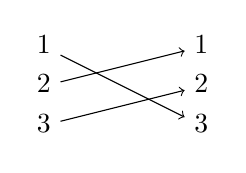
\begin{tikzpicture}
            \foreach[count=\i] \lseti/\lsetmi in {A/{1,2,3},B/{1,2,3}} {
                \begin{scope}[local bounding box=\lseti, x=2cm, y=0.5cm]
                \foreach[count=\j] \lj in \lsetmi {
                    \node[minimum width=1em,anchor=base,text height=1.4ex,text
                    depth=0.25ex] (n-\j-\lseti) 
                    at (\i,-\j) {\lj};
                }
                \end{scope}
                % \node[ellipse, draw, fit=(\lseti), 
                % label={[name=l-\lseti]above:$\lseti$}] {};
            }
            \draw[->] (n-1-A) -- (n-3-B);
            \draw[->] (n-2-A) -- (n-1-B);
            \draw[->] (n-3-A) -- (n-2-B);
        \end{tikzpicture}
        \caption*{\(\sigma\)}
        \endminipage\hfill
        \minipage{0.32\textwidth}
        \centering
        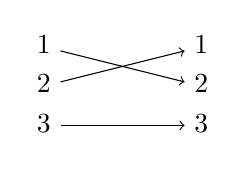
\begin{tikzpicture}
            \foreach[count=\i] \lseti/\lsetmi in {A/{1,2,3},B/{1,2,3}} {
                \begin{scope}[local bounding box=\lseti, x=2cm, y=0.5cm]
                \foreach[count=\j] \lj in \lsetmi {
                    \node[minimum width=1em,anchor=base,text height=1.4ex,text
                    depth=0.25ex] (n-\j-\lseti) 
                    at (\i,-\j) {\lj};
                }
                \end{scope}
                % \node[ellipse, draw, fit=(\lseti), 
                % label={[name=l-\lseti]above:$\lseti$}] {};
            }
            \draw[->] (n-1-A) -- (n-2-B);
            \draw[->] (n-2-A) -- (n-1-B);
            \draw[->] (n-3-A) -- (n-3-B);
        \end{tikzpicture}
        \caption*{\(\tau\)}
        \endminipage\hfill
        \minipage{0.32\textwidth}%
        \centering
        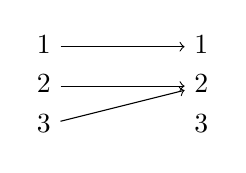
\begin{tikzpicture}
            \foreach[count=\i] \lseti/\lsetmi in {A/{1,2,3},B/{1,2,3}} {
                \begin{scope}[local bounding box=\lseti, x=2cm, y=0.5cm]
                \foreach[count=\j] \lj in \lsetmi {
                    \node[minimum width=1em,anchor=base,text height=1.4ex,text
                    depth=0.25ex] (n-\j-\lseti) 
                    at (\i,-\j) {\lj};
                }
                \end{scope}
                % \node[ellipse, draw, fit=(\lseti), 
                % label={[name=l-\lseti]above:$\lseti$}] {};
            }
            \draw[->] (n-1-A) -- (n-1-B);
            \draw[->] (n-2-A) -- (n-2-B);
            \draw[->] (n-3-A) -- (n-2-B);
        \end{tikzpicture}
        \caption*{Not a permutation.}
        \endminipage
        \end{figure}
        Notice that \(\sigma\) and \(\tau\) are permutations. The obvious way to compute the product is to list:
        \[1\mapsto 3\mapsto 3\]
        \[2\mapsto 1\mapsto 2\]
        \[\underbrace{3\mapsto 2\mapsto 1}_{\tau\circ\sigma}\]
\end{example}
\begin{definition}
    Any list of \(k\) different elements \(a_1,a_2,\ldots,a_k\in\{1,\ldots,n\}\) determines a \emph{\(k\)-cycle} \(\sigma=(a_1a_2\cdots a_k)\) as follows.
    \[\sigma(b)=\begin{cases}
        a_{j+1} & b=a_j,j<k \\
        a_1 & b=a_k \\
        b & \text{otherwise}
    \end{cases}\]
\end{definition}
With cycles, we can easily calculate the product of permutations. 
\begin{example}
    Consider \(\sigma=(132)=(321)\), \(\tau=(12)\). Then 
    \[\tau\sigma=(12)(132)=(13)(2)=(13)\]
\end{example}
\begin{example}
    \((1432)(243)=(1423)\).
\end{example}
\begin{remark}
    Note that \((a_1a_2\cdots a_k)=(a_2a_3\cdots a_ka_1)\). For example,
    \[(123)=(231)=(312)\]
\end{remark}
\begin{definition}
    Cycles \((a_1\cdots a_k)\) and \((b_1\cdots b_k)\) are \emph{disjoint} if \(a_i\neq b_j\) for all \(i,j\).
\end{definition}
For example, \((123),(45)\in S_5\) are disjoint. N.b. disjoint cycles commute.
\begin{theorem}
    Every \(\sigma\in S_n\) can be written as a product of disjoint cycles. This expression is unique up to:
    \begin{enumerate}
        \item Shifting the element of each cycle.
        \item Permuting the cycles.
    \end{enumerate}
\end{theorem}
\begin{proof}
    The action of \(\langle\sigma\rangle\) on \(X=\{1,\ldots,n\}\) partition \(X\) into orbits:
    \[\langle\sigma\rangle i_1\cup\langle\sigma\rangle i_2\cup\cdots\cup\langle\sigma\rangle i_k\]
    Setting \(n_j=|\langle\sigma\rangle i_j|\) for \(1\leq j\leq k\), we see that 
    \[\sigma=(i_1\:\sigma(i_1)\cdots\sigma^{n_1-1}(i_1))(i_2\cdots\sigma^{n_2-1}(i_2))\cdots(i_k\cdots\sigma^{n_k-1}(i_k))\]
    which proves existence. (These are all disjoint because orbits partition.) For uniqueness, note that the only choices we made were (1) orbit representative \(i_j\), and (2) the order in which we wrote down the orbits. But changing (1) shifts the cycle, and changing (2) permutes the cycles.
\end{proof}
\begin{example}
    \((12)(34)(56)(123456)=(1)(246)(3)(5)=(246)\)
\end{example}
\begin{definition}
    If \(\sigma=(a_1^1\cdots a_{k_1}^1)\cdots(a_1^l\cdots a_{k_l}^l)\) are disjoint cycles, then \(\sigma\) is called a \emph{\((k_1,\ldots,k_l)-cycle\)}. The set of numbers \(\{k_1,\ldots,k_l\}\) is called the \emph{cycle type} of \(\sigma\).
\end{definition}
For example, \((12)(34)(56)\) is a \((2,2,2)\)-cycle. We usually omit singletons, so, e.g. \((12)(345)(6)\) is a \((2,3)\)-cycle.
\begin{remark}
    If \(\sigma=(a_1\cdots a_k)\) is a \(k\)-cycle, then \(o(\sigma)=k\). More generally, if \(\sigma\) is a \((k_1,\ldots,k_l)\)-cycle, then \(o(\sigma)=\text{lcm}\{k_1,\ldots,k_l\}\).
\end{remark}
\begin{definition}
    A \(2\)-cycle is called a \emph{transposition}.
\end{definition}
\begin{theorem}
    The set of transposition in \(S_n\) generates \(S_n\).
\end{theorem}
\begin{proof}
   Note there is a copy of \(S_{n-1}\) sitting inside \(S_n\) as a subgroup: \(S_{n-1}\cong\stab_{S_n}(n)\). The proof is by induction on \(n\). 
   
   For base case \(n=2\), \(S_2=\{e,(1,2)\}\cong C_2\) and the result is obvious. Now suppose \(S_{n-1}\) is generated by transposition, and let \(\sigma\in S_n\). If \(\sigma(n)=n\), then \(\sigma\in\stab_{S_n}(n)\cong S_{n-1}\) so \(\sigma\) is a product of transpositions by the inductive hypothesis. If not, let \(\tau=(n\:\sigma(n))\). Then 
    \[\tau\sigma(n)=\tau(\sigma(n))=n\]
    So, as above, 
    \[\tau\sigma\in\stab_{S_n}(n)\cong S_{n-1}\]
    and \(\tau\sigma\) is a product of transpositions. Thus \(\sigma\) is also a product of transpositions.
\end{proof}
In fact, we can do slightly better. A transposition of the form \((i\:i+1)\) is for \(1\leq i<n\) is called \emph{adjacent}. Then, we have the following.
\begin{lemma}
    Any transposition is a product of odd numbers of adjacent transpositions.
\end{lemma}
\begin{proof}
    Let \((ij)\) be a transposition with \(j>i\). We proceed by induction on \(j-i\).

    In the base case, \(j=i+1\Rightarrow (ij)=(i\:i+1)\) is adjacent. Otherwise, if \(j>i+1\), then
    \[(j-1\:j)(i\:j-1)(j-1\:j)=(ij)\]
    and the result follows by induction.
\end{proof}
\begin{lemma}
    If \(\tau_1,\ldots,\tau_k\) are all transpositions, and 
    \[\sigma=\tau_1\cdots\tau_k=e\] then \(k\) is even.
    \label{lemma:transpo_even}
\end{lemma}
\begin{proof}
    First, note that we may assume that all the \(\tau_i\) are adjacent.\footnote{Parity is conserved.} Also, we call a pair \(\{i,j\}\subseteq\{1,\ldots,n\}\) an \emph{inversion} if \(i<j\) but \(\sigma(i)>\sigma(j)\). The lemma follows from the claim: 
    \[k\equiv\hash\text{  inversions of  }\sigma\mod 2\]
    We prove the claim by induction on \(k\). Base case is when \(k=0\), numbers of inversion \(0\). Now suppose 
    \[\sigma=\tau_1\tau_2\cdots\tau_k=\tau\sigma^\prime\]
    with \(\tau_1=\tau=(l\:l+1)\), \(\sigma^\prime=\tau_2\cdots\tau_k\).
    How many pairs \(\{i,j\}\) (\(i<j\)) are inversions of \(\sigma^\prime\) but not \(\sigma\), or vice versa? There are 10 cases to analyse, depending on where \(l\) and \(l+1\) are, relative to \(\sigma^\prime(i)\), \(\sigma^\prime(j)\).
    \begin{table}[H]
        \centering
        \begin{tabularx}{0.45\textwidth}{ccX}
            \toprule
            \(\sigma^\prime\) & \(\sigma\) & order \\
            \midrule
            \xmark & \xmark & \(l<l+1\leq\sigma^\prime(i)<\sigma^\prime(j)\) \\
            \checkmark & \checkmark & \(l<l+1\leq\sigma^\prime(j)<\sigma^\prime(i)\) \\
            \xmark & \xmark & \(\sigma^\prime(i)<\sigma^\prime(j)\leq l<l+1\) \\
            \checkmark & \checkmark & \(\sigma^\prime(j)<\sigma^\prime(i)\leq l<l+1\) \\
            \xmark & \xmark & \(\sigma^\prime(i)\leq l<l+1<\sigma^\prime(j)\) \\
            \checkmark & \checkmark & \(\sigma^\prime(j)\leq l<l+1\leq\sigma^\prime(i)\) \\
            \xmark & \xmark & \(\sigma^\prime(i)<l<l+1\leq\sigma^\prime(j)\) \\
            \checkmark & \checkmark & \(\sigma^\prime(j)<l<l+1\leq\sigma^\prime(i)\) \\
            \xmark & \checkmark & \(\sigma^\prime(i)=l<l+1=\sigma^\prime(j)\) \\
            \checkmark & \xmark & \(\sigma^\prime(j)=l<l+1=\sigma^\prime(i)\) \\
            \bottomrule 
        \end{tabularx}
    \end{table}
    Since the final two cases correspond to the unique pair \(\{(\sigma^\prime)^{-1}(l),(\sigma^\prime)^{-1}(l+1)\}\), 
    \[\hash\text{  inversions of  }\sigma=(\hash\text{  inversions of  }\sigma^\prime)\pm 1\]
    proving the claim. Now, if \(\sigma=\tau_1\cdots\tau_k=2\), then \(\sigma\) has 0 inversions, so by the claim, \(k\equiv 0\mod 2\), i.e. \(k\) is even.
\end{proof}
\begin{theorem}
    (\emph{Sign Homomorphism}) The map \[\sgn:S_n\to C_2=\{\pm 1\},\quad\tau_1\cdots\tau_k\mapsto (-1)^k\] is a well defined homomorphism.
\end{theorem}
\begin{proof}
    To see that \(\sgn\) is well defined, suppose \(\tau_i,\tau_j^\prime\) are transpositions such that \(\tau_1\cdots\tau_k=\tau_1^\prime\cdots\tau_l^\prime\). Then,
    \[\tau_k\tau_{k-1}\cdots\tau_1\tau_1^\prime\cdots\tau_l^\prime=e\]
    But by Lemma \ref{lemma:transpo_even} above, \(k+l\) is a multiple of \(2\). Hence, \(k\equiv l\mod 2\Rightarrow (-1)^k=(-1)^l\).

    Now, to see that \(\sgn\) is a homomorphism, note that 
    \begin{align*}
        \sgn(\tau_1\cdots\tau_k\tau_1^\prime\cdots\tau_l^\prime)&=(-1)^{k+l}=(-1)^k(-l)^l \\
        &=\sgn(\tau_1\cdots\tau_k)\sgn(\tau_1^\prime\cdots\tau_l^\prime)
    \end{align*}
\end{proof}
\begin{definition}
    If \(\sgn(\sigma)=1\), then \(\sigma\) is \emph{even}; otherwise, \(\sigma\) is called \emph{odd}. The subgroup containing even permutations, i.e. 
    \[A_n=\ker(\sgn)\lhd S_n\]
    is called the \emph{alternating group} on \(n\) elements.
\end{definition}
\begin{example}
    \(S_3=\{e,(123),(321),(12),(23),(31)\}\). We have \((123)=(12)(23)\) and \((321)=(23)(12)\). Therefore,
    \[A_3=\{e,(123)(321)\}\cong C_3\]
\end{example}
\begin{remark}
    The cycle type makes it easy to determine the sign of a permutation. Indeed, 
    \[(a_1\cdots a_k)=(a_1a_k)(a_1a_{k-1})\cdots(a_1a_3)(a_1a_2)\]
    so \((a_1\cdots a_k)\) is even if and only if \(k\) is odd. More generally, a \((k_1,\ldots,k_l)\)-cycle is even if and only if \(\hash\{k_i\text{  even}\}\) is even.
\end{remark}
\begin{example}
    \((12)(34)\) is even but \((12)(34)(56)\) is odd.
\end{example}
Let's apply the facts to study conjugation in \(S_n\) and \(A_n\). We will start with \(S_n\).
\begin{theorem}
    Two permutations \(\sigma_1,\sigma_2\in S_n\) are conjugate if and only if their cycle types are the same.
    \label{thm:permu_conj}
\end{theorem}
\begin{proof}
    Suppose \[\sigma_1=(a_1^1\cdots a_{l_1}^1)\cdots(a_1^k\cdots a_{l_k}^k)\] is a product of disjoint cycles, so \[\sigma_1(a_j^i)=a_{j+_{l_i}1}^i\] Since the cycle types are same, \(\sigma_2\) will take the form \(\sigma_2=(b_1^1\cdots b_{l_1}^1)\cdots(b_1^k\cdots b_{l_k}^k)\). Now, note that \(\tau(a_j^i)=b_j^i\) defines a permutation of \(\{1,\ldots,n\}\). Let's compute 
    \[\tau\sigma_1\tau^{-1}(b_j^i)=\tau\sigma_1(a_j^i)=\tau(a_{j+_{l_i}+1}^i)=b_{j+_{l_i}1}^i\]
    Hence \(\tau\sigma_1\tau^{-1}=\sigma_2\). So \(\sigma_1\) and \(\sigma_2\) are indeed conjugate.

    Conversely, suppose \(\sigma_2=\tau\sigma_1\tau^{-1}\). The above argument says that if \[\sigma_1=(a_1^1\cdots a_{l_1}^1)\cdots(a_1^k\cdots a_{l_k}^k)\] then 
    \[\sigma_2=(b_1^1\cdots b_{l_1}^1)\cdots(b_1^k\cdots b_{l_k}^k)\]
    where \(b_j^i=\tau(a_j^i)\). Therefore, \(\sigma_1\) and \(\sigma_2\) have the same cycle type.
\end{proof}
\begin{proposition}
    Sign homomorphism is the only surjective homomorphism from \(S_n\) to \(C_2\). 
\end{proposition}
\begin{proof}
    Since any two transpositions are conjugate, for arbitrary transpositions \(\tau^\prime\) and \(\tau\), there exists \(\sigma\in S_n\) such that 
    \[\tau^\prime=\sigma\tau\sigma^{-1}\]
    If we let \(\phi:S_n\to C_2\) a surjective homomorphism,
    \[\phi(\tau^\prime)=\phi(\sigma\tau\sigma^{-1})=\phi(\tau)\]
    Also, since any permutations be written as product of transpositions,
    \[\phi(g)=\phi(\tau_1\cdots\tau_k)=(\phi(\tau_1))^k\]
    and for \(\phi\) to be surjective, \(\phi(\tau_1)=-1\) and thus \(\phi=\sgn\).
\end{proof}
\begin{example}
    \((12)(123)(12)=(213)\); and, more generally, 
    \[\sigma(12\cdots l)\sigma^{-1}=\left(\sigma(1)\;\sigma(2)\cdots\sigma(l)\right)\]
\end{example}
We can use Theorem \ref{thm:permu_conj} to count conjugacy classes in \(S_n\).
\begin{example}
    \(|\ccl_{S_3}(12)|=\binom 32=3\), \(|\ccl_{S_3}(123)|=2\), and \(|\ccl_{S_3}((12)(34))|=3\).
\end{example}
Recall that orbit-stabiliser (Corollarly \ref{coro:orbit_stab}) tells us that 
\[|C_{S_n}(\sigma)|=|S_n|/|\ccl_{S_n}(\sigma)|=n!/|\ccl_{S_n}(\sigma)|\]
Hence we can also compute the sizes of centralisers.
\begin{example} Consider \(S_4\).
    \[|C_{S_4}((12)(34))|=\frac{|S_4|}{|\ccl_{S_4}((12)(34))|}=\frac{4!}{3}=8\]
    Indeed, we can list 
    \[C_{S_4}((12)(34))=\{e,(12),(34),(12)(34),(13)(24),(14)(23),(1423),(1324)\}\]
\end{example}
\begin{example}
    We can list all the conjugacy classes in \(S_4\) as follows.
    \begin{table}[H]
        \centering
        \begin{tabularx}{0.6\textwidth}{Xcc}
            \toprule
            Typical element \(\gamma\) & \(|\ccl_{S_4}(\gamma)|\) & \(|C_{S_4}(\gamma)|\) \\
            \midrule
            \(e\) & 1 & 24 \\
            \((12)\) & 6 & 4 \\
            \((12)(34)\) & 3 & 8 \\
            \((123)\) & 8 & 3 \\
            \((1234)\) & 6 & 4 \\
            \bottomrule 
        \end{tabularx}
    \end{table}
    and check \(|S_4|=24\) if wanted.
    \label{eg:conj_s4}
\end{example}
Now, let's turn to conjugacy classes in \(A_n\). Be careful, that conjugacy classes in \(S_n\) can split in \(A_n\). Note that, by the isomorphism theorem (Theorem \ref{thm:isom}), 
\[S_n/A_n\cong C_2\]
and 
\[|S_n|=|S_n/A_n||A_n|=2|A_n|\]
by Lagrange's theorem.
\begin{example}
    \((123),(321)\) are conjugate in \(S_3\). But \(A_3\cong C_3\) is abelian, so \((123)\) is not conjugate in \(A_3\) to \((321)\), because they are not equal.\footnote{There is no permutation \(\tau\) in \(A_n\) such that \(\tau(123)\tau^{-1}=(321)\).}
\end{example}
\begin{lemma}
    Let \(\gamma\in A_n\subseteq S_n\).
    \begin{enumerate}
        \item If some odd element of \(S_n\) commutes with \(\gamma\), then \(\ccl_{A_n}(\gamma)=\ccl_{S_n}(\gamma)\).
        \item If every element of \(S_n\) that commutes with \(\gamma\) is even, then \(\ccl_{S_n}(\gamma)\) splits into two:
        \[\ccl_{S_n}(\gamma)=\ccl_{A_n}(\gamma)\cup\ccl_{A_n}(\tau\gamma\tau)\]
        where \(\tau\) is any transposition.
    \end{enumerate}
\end{lemma}
\begin{proof}
    Orbit-stabiliser gives \(|S_n|=|\ccl_{S_n}(\gamma)||C_{S_n}(\gamma)|\), \(|A_n|=|\ccl_{A_n}(\gamma)||C_{A_n}(\gamma)|\). \\ Since \(|S_n|=2|A_n|\), 
    \[|\ccl_{S_n}(\gamma)|=\frac{2|C_{A_n}(\gamma)|}{|C_{S_n}(\gamma)|}|\ccl_{A_n}(\gamma)|\]
    Now, \(C_{A_n}(\gamma)=C_{S_n}(\gamma)\cap A_n\) by definition; so 
    \[|C_{S_n}(\gamma):C_{A_n}(\gamma)|\leq 2\]
    (because \(|S_n:A_n|=2\)).\footnote{Draw a diagram if confused.}
    We take a look at two conditions from the lemma.
    \begin{enumerate}
        \item If there is an odd element of \(S_n\) that commutes with \(\gamma\), then \(|C_{S_n}(\gamma):C_{A_n}(\gamma)|=2\). So, \(|\ccl_{S_n}(\gamma)|=|\ccl_{A_n}(\gamma)|\) by Lagrange's theorem and \(\ccl_{S_n}(\gamma)=\ccl_{A_n}(\gamma)\) since \(\ccl_{A_n}(\gamma)\subseteq\ccl_{S_n}(\gamma)\).
        \item The hypothesis means that \(C_{S_n}(\gamma)=C_{A_n}(\gamma)\). So \(|\ccl_{S_n}(\gamma)|=2|\ccl_{A_n}(\gamma)|\) and \(|\ccl_{S_n}(\gamma)|\) splits into two. Now, consider a transposition \(\tau\in S_n\). Note that \(\tau\gamma\tau^{-1}\in\ccl_{S_n}(\gamma)\). We need to prove that \(\tau\gamma\tau^{-1}\) and \(\gamma\) are not conjugate in \(A_n\). If they were, then there would be \(\alpha\in A_n\) such that 
        \[\tau\gamma\tau^{-1}=\alpha\gamma\alpha^{-1}\Rightarrow(\alpha^{-1}\tau)\gamma=\gamma(\alpha^{-1}\tau)\]
        so \(\alpha^{-1}\tau\) is an odd element of \(S_n\) that commutes with \(\gamma\), which is a contradiction.
    \end{enumerate}
\end{proof}
This makes it possible to determine conjugacy classes in \(A_n\).
\begin{example}
    Consider \(A_4\). All even elements of \(S_4\) are \((2,2)\)-cycles or \(3\)-cycles. Recall that \((12)\) commutes with \((12)(34)\); so \(\ccl_{S_4}((12)(34))\) does not split. For a \(3\)-cycle, \(\sigma=(123)\), we have \(|C_{S_n}(123)|=3\) from Example \ref{eg:conj_s4}, so 
    \[C_{S_4}\left((123)\right)=\{2,(123),(321)\}\subseteq A_4\]
    and the conjugacy class splits. In summary,
    \begin{table}[H]
        \centering
        \begin{tabularx}{0.6\textwidth}{Xcc}
            \toprule
            Typical element \(\gamma\) & \(|\ccl_{A_4}(\gamma)|\) & \(|C_{A_4}(\gamma)|\) \\
            \midrule
            \(e\) & 1 & 12 \\
            \((12)(34)\) & 3 & 4 \\
            \((123)\) & 4 & 3 \\
            \((321)\) & 4 & 3 \\
            \bottomrule 
        \end{tabularx}
    \end{table}
\end{example}
Finally, let's perform a similar calculation for \(S_5\) and \(A_5\).
\begin{example}
    For \(S_5\), we have the conjugacy classes as follows.
    \begin{table}[H]
        \centering
        \begin{tabularx}{0.6\textwidth}{Xcc}
            \toprule
            Typical element \(\gamma\) & \(|\ccl_{S_5}(\gamma)|\) & \(|C_{S_5}(\gamma)|\) \\
            \midrule
            \(e\) & 1 & 120 \\
            \((12)\) & 10 & 12 \\
            \((123)\) & 20 & 6 \\
            \((12)(34)\) & 15 & 8 \\
            \((123)(45)\) & 20 & 6 \\
            \((1234)\) & 30 & 4 \\
            \((12345)\) & 24 & 5 \\
            \bottomrule 
        \end{tabularx}
    \end{table}
    Note that even cycles are \(\{e,(123),(12)(34),(12345)\}\subseteq A_5\). We take a closer look at each of them.
    \begin{itemize}
        \item \((45)\in C_{S_5}(123)\) so \(\ccl_{S_5}(123)\) does not split.
        \item \((12)\in C_{S_5}((12)(34))\) so \(\ccl_{S_5}((12)(34))\) does not split.
        \item \(|C_{S_5}(12345)|=5\) and \(C_{S_5}(12345)\supseteq\langle(12345)\rangle\cong C_5\). Hence \(C_{S_5}(12345)=\langle (12345)\rangle\subseteq A_5\)
         and \(\ccl_{S_5}(12345)\) splits.
    \end{itemize}
    In summary,
    \begin{table}[H]
        \centering
        \begin{tabularx}{0.6\textwidth}{Xcc}
            \toprule
            Typical element \(\gamma\) & \(|\ccl_{A_5}(\gamma)|\) & \(|C_{A_5}(\gamma)|\) \\
            \midrule
            \(e\) & 1 & 60 \\
            \((123)\) & 20 & 3 \\
            \((12)(34)\) & 15 & 4 \\
            \((12345)\) & 12 & 5 \\
            \((21345)\) & 12 & 5 \\
            \bottomrule 
        \end{tabularx}
    \end{table}
\end{example}
\begin{theorem}
    \(A_5\) is simple.
\end{theorem}
\begin{proof}
    Suppose \(N\lhd A_5\). We need to prove that \(N=1\) or \(N=A_5\). By Example Sheet 3 Q5, \(N\) is an union of conjugacy classes of \(A_5\). Since it has to contain \(e\), the possible orders of \(N\) are: 1, 21, 36, 48, 33, 45, 16, 28, 40, 13, 25, 60. By Lagrange's theorem, only acceptable values are 1 and 60, which correspond to trivial subgroup and \(A_5\) respectively. Hence, \(A_5\) is indeed simple. (Also note that \(A_5\) is the smallest example of a non-abelian simple group).
\end{proof}
\section{Matrix Groups}
This section requires some knowledge from Vectors \& Matrices.
\subsection{General Linear Group}
Groups of matrices provide some of the most important and fascinating examples of (infinite) groups. To begin, let 
\[M_n(\mathbb{F})=\{n\times n\text{  matrices with entries in  }\mathbb{F}\}\]
where \(\mathbb{F}\) a field, e.g. \(\mathbb{R},\mathbb{C}\). Matrix multiplication is well known to be associative, and there is an identity \(I_n=I=\mathbb{1}=1\). However, not all matrices are invertible.
\begin{definition}
    A \emph{general linear group} \(\GL(n,\mathbb{F})\) is defined as a set of invertible \(n\times n\) matrices over \(\mathbb{F}\).\footnote{Composition of invertible matrices are invertible.}
\end{definition}
\begin{proposition}
    \(\det:\GL(n,\mathbb{F})\to\mathbb{F}\backslash\{0\}\) is a surjective homomorphism.
\end{proposition}
\begin{proof}
    We have \(\det AB=\det A\det B\). Also, if \(A\) invertible, it has non-zero determinant and \(\det A\in\mathbb{F}\backslash\{0\}\). Furthermore, to prove surjectivity, for any \(x\in\mathbb{F}\backslash\{0\}\), we take \(I\) and replace \(I_{11}\) with \(x\). Then the determinant of such matrix is \(x\).
\end{proof}
\begin{definition}
    We define the \emph{special linar group} as the kernel of \(\det:\GL(n,\mathbb{F})\to\mathbb{F}\backslash\{0\}\):
    \[\SL(n,\mathbb{F})=\ker(\det)=\{A\in\GL\:|\:\det A=1\}\]
\end{definition}
It follows that \(\SL(n,\mathbb{F})\lhd\GL(n,\mathbb{F})\). Also note that \(Q_8\leq\SL(2,\mathbb{C})\).
\subsection{Change of Basis and Action}
One may think of a natural action by matrix conjugation:
\[\GL(n,\mathbb{R})\acts M_n(\mathbb{R}),\quad P(A)=PAP^{-1}\]
where \(P\in\GL(n,\mathbb{R})\) and \(A\in M_n(\mathbb{R})\).
\begin{proposition}
    Let \(V\) be a \(n\)-dimensional vector space and \(\alpha:V\to V\) a linear map. If \(A\in M_n(\mathbb{R})\) represents \(\alpha\) in some basis, then the orbit 
    \[\GL(n,\mathbb{R})A=\{PAP^{-1}\:|\:P\in\GL(n,\mathbb{R})\}\]
    consists of all matrices that represent \(\alpha\) in any basis.
\end{proposition}
\begin{proof}
    A basis \(\{\mathbf{v}_1,\ldots,\mathbf{v}_n\}\) for \(V\) defines an isomorphisms of vector spaces \(\phi:\mathbb{R}^n\to V\),
    \[(\lambda_1,\ldots,\lambda_n)\mapsto\sum_{i=1}^n\lambda_i\mathbf{v}_i\]
    The hypothesis that \(A\) represents \(\alpha\) in this basis means:
    \[A=\phi^{-1}\circ\alpha\circ\phi\Rightarrow\alpha=\phi\circ A\circ\phi^{-1}\]
    Likewise, another basis \(\{u_1,\ldots,u_n\}\) corresponds to an isomorphism \(\psi:\mathbb{R}^n\to V\) and \(B\in M_n(\mathbb{R})\) reprents \(\alpha\) in this basis if 
    \[B=\psi^{-1}\circ\alpha\circ\psi=\psi^{-1}\circ(\phi\circ A\circ\phi^{-1})\circ\psi=(\psi^{-1}\circ\phi)\circ A\circ(\psi^{-1}\circ\phi)^{-1}\]
    Thus, \(B=PAP^{-1}\) where \(P=\psi^{-1}\circ\phi\in\GL(n,\mathbb{R})\). We have shown that every matrix representing \(\alpha\) is in \(\GL(n,\mathbb{R})\). We still need to prove the reverse inclusion.

    Conversely, suppose \(B=PAP^{-1}\). Then, setting \(\psi=\phi\circ P^{-1}\), it defines a basis 
    \[\{\mathbf{u}_i=\psi(\mathbf{e}_i)\}\]
    for \(V\) with \(\mathbf{e}_i\) as the standard \(i\)\textsuperscript{th}
    basis vector of \(\mathbb{R}^n\). Then, \(B\) is the matrix for \(\alpha\) in this basis.
\end{proof}
\subsection{Möbius Transformation Revisited}
Recall that multiplication in \(\mathcal{M}\) looked similar to multiplication of \(2\times 2\) matrices. This is explained by the next result.
\begin{proposition}
    Identitify 
    \[\mathbb{C}_\times=\left\{\left.\begin{pmatrix}
        \lambda & 0 \\ 0 & \lambda
    \end{pmatrix}\in\GL(2,\mathbb{C})\:\right|\:\lambda\neq 0\right\}\]
    Then \(\mathbb{C}_\times\lhd\GL(2,\mathbb{C})\) and \(\GL(2,\mathbb{C})/\mathbb{C}_\times\cong\mathcal{M}\).
\end{proposition}
\begin{proof}
    Define \(\Phi:\GL(2,\mathbb{C})\to\mathcal{M}\), 
    \[\begin{pmatrix}
        a & b \\ c & d
    \end{pmatrix}\mapsto\left(z\mapsto\frac{az+b}{cz+d}\right)\]
    By our computation of multiplication in \(\mathcal{M}\), we see that \(\Phi\) is a homomorphism, which is obviously surjective. A matrix 
    \[\begin{pmatrix}
        a & b \\ c & d
    \end{pmatrix}\in\ker\Phi\]
    if and only if it fixes \(0,1,\infty\), i.e. \(b=c\) and \(a+b=c+d\Rightarrow a=d\). So \(\ker\Phi=\mathbb{C}_\times\). The result follows from the isomorphism theorem (Theorem \ref{thm:isom}).
\end{proof}
\subsection{Orthogonal Groups}
Let's write \(||\bullet ||\) for the usual Euclidean notation of distance on \(\mathbb{R}^n\):
\[||\mathbf{u}-\mathbf{v}||=\sqrt{\sum_{i=1}^{n}(u_i-v_i)^2}\]
\begin{definition}
    The \(n\)-dimensional \emph{orthogonal group} is the subgroup of \(\GL(n,\mathbb{R})\) that preserves distance in \(\mathbb{R}^n\), i.e.
    \[\text{O}(n)=\{A\in\GL(n,\mathbb{R})\::\:||A\mathbf{u}-A\mathbf{v}||=||\mathbf{u}-\mathbf{v}||,\quad\forall \mathbf{u,v}\in\mathbb{R}^n\}\]
\end{definition}
\begin{remark}
    This is same as saying that \(||A\mathbf{x}||=||\mathbf{x}||\) for all \(\mathbf{x}\in\mathbb{R}^n\). In fact, the \emph{dot product}
    \[\mathbf{u}\cdot\mathbf{v}=\sum_{i=1}^nu_iv_i\]
    is often more convinient to work with the notion of distance.
\end{remark}
\begin{lemma}
    (\emph{Polarisation Identity}) For \(\mathbf{u},\mathbf{v}\in\mathbb{R}^n\), 
    \[2(\mathbf{u}\cdot\mathbf{v})=||\mathbf{u}||^2+||\mathbf{v}||^2-||\mathbf{u}-\mathbf{v}||^2\]
\end{lemma}
\begin{proof}
    By definitions,
    \[||\mathbf{u}-\mathbf{v}||^2=(\mathbf{u}-\mathbf{v})\cdot(\mathbf{u}-\mathbf{v})=||\mathbf{u}||^2-2(\mathbf{u}\cdot\mathbf{v})+||\mathbf{v}||^2\]
\end{proof}
Hence, we can characterise \(\mathrm{O}(n)\) using the dot product.
\begin{lemma}
    \[\mathrm{O}(n)=\{A\in\GL(n,\mathbb{R})\:|\:(A\mathbf{x})\cdot(A\mathbf{y})=\mathbf{x}\cdot\mathbf{y},\quad\forall\mathbf{x},\mathbf{y}\in\mathbb{R}^n\}\]
\end{lemma}
\begin{proof}
    If \((A\mathbf{x})\cdot(A\mathbf{y})=\mathbf{x}\cdot\mathbf{y}\) for all \(\mathbf{x},\mathbf{y}\in\mathbb{R}^n\), then, for any \(\mathbf{u},\mathbf{v}\in\mathbb{R}^n\),
    \[||A\mathbf{u}-A\mathbf{v}||^2=||A(\mathbf{u}-\mathbf{v})||^2=(A(\mathbf{u}-\mathbf{v}))\cdot(A(\mathbf{u}-\mathbf{v}))=(\mathbf{u}-\mathbf{v})\cdot(\mathbf{u}-\mathbf{v})=||\mathbf{u}-\mathbf{v}||^2\]
    so \(A\in\mathrm{O}(n)\).

    Conversely, if \(A\in\mathrm{O}(n)\), then for any \(\mathbf{x},\mathbf{y}\in\mathbb{R}^n\),
    \begin{align*}
        2(A\mathbf{x})\cdot(A\mathbf{y})&=||A\mathbf{x}||^2+||A\mathbf{y}||^2-||A\mathbf{x}-A\mathbf{y}||^2 \\
        &=||A\mathbf{x}-A0||^2+||A\mathbf{y}-A0||^2-||A\mathbf{x}-A\mathbf{y}||^2 \\
        &=||\mathbf{x}||^2+||\mathbf{y}||^2-||\mathbf{x}-\mathbf{y}||^2=2(\mathbf{x}\cdot\mathbf{y})
    \end{align*}
    using the polarisation identity.
\end{proof}
\begin{lemma}
    Let \(A\in M_n(\mathbb{R})\). Then following are equivalent:
    \begin{enumerate}
        \item \(A\in\mathrm{O}(n)\);
        \item The columns of \(A\) forms an orthonormal basis;
        \item \(A^\intercal A=I\).
    \end{enumerate}
\end{lemma}
\begin{proof}
    (1)\(\Rightarrow\)(2). Let \(\{\mathbf{e}_1,\ldots\mathbf{e}_n\}\) be the standard basis for \(\mathbb{R}^n\). The \(i\)\textsuperscript{th} column of \(A\) is \(A\mathbf{e}_i\). But 
    \[(A\mathbf{e}_i)\cdot(A\mathbf{e}_j)=\mathbf{e}_i\cdot\mathbf{e}_j=\delta_{ij}\]
    so the columns form an orthonormal basis.

    (2)\(\Rightarrow\)(3). Since \((A\mathbf{e}_i)\cdot(A\mathbf{e}_j)=\mathbf{e}_i\cdot\mathbf{e}_j=\delta_{ij}\), \(\mathbf{u}\cdot\mathbf{v}=\mathbf{u}^\intercal\mathbf{v}\), this means that \(e_i^\intercal A^\intercal Ae_j=\delta_{ij}\). But \(\mathbf{e}_i^\intercal M\mathbf{e}_j\) is the \(ij\) entry of \(M\) for any matrix \(M\), so \(A^\intercal A=I\) as required.

    (3)\(\Rightarrow\)(1). Suppose \(\mathbf{u},\mathbf{v}\in\mathbb{R}^n\). Then 
    \[(A\mathbf{u})\cdot(A\mathbf{v})=(A\mathbf{u})^\intercal(A\mathbf{v})=\mathbf{u}^\intercal A^\intercal A\mathbf{v}=\mathbf{u}^\intercal\mathbf{v}=\mathbf{u}\cdot\mathbf{v}\]
\end{proof}
Recall that \(\det(A^\intercal)=\det A\). Therefore, if \(A\in\mathrm{O}(n)\), 
\[1=\det I=\det(A^\intercal A)=\det(A^\intercal)\det A=(\det A)^2\]
Hence \(\det A=\pm 1\). 
\begin{definition}
    We define the \emph{special orthogonal group} as 
    \[\SO(n)=\mathrm{O}(n)\cap\SL(n,\mathbb{R})=\{A\in\mathrm{O}(n)\:|\:\det A=1\}\]
\end{definition}
Note that \(\SO(n)=\ker(\det:\mathrm{O}(n)\to\{\pm 1\})\) so 
\[|\mathrm{O}(n):\SO(n)|=2\]
by the isomorphism theorem.
\begin{definition}
    Any \(\mathbf{v}\in\mathbb{R}^n\backslash\{0\}\) defines an orthogonal (hyper) plane 
    \[P_\mathbf{v}=\{\mathbf{x}\in\mathbb{R}^n\:|\:\mathbf{x}\cdot\mathbf{v}=0\}\]
    The \emph{reflection} of \(\mathbf{x}\) in \(P_\mathbf{v}\) is defined to be 
    \[S_\mathbf{v}(\mathbf{x})=\mathbf{x}-\frac{2(\mathbf{x}\cdot\mathbf{v})\mathbf{v}}{||\mathbf{v}||^2}\]
\end{definition}
\begin{remark}
    We may replace \(\mathbf{v}\) by \(\mathbf{v}/||\mathbf{v}||\). Hence, without loss of generality, we may assume that \(||\mathbf{v}||=1\). We may also abuse notation and write \(S_P\) to denote reflection in the plane \(P\).
\end{remark}
\begin{lemma}
    For a reflection \(S_\mathbf{v}\), \(S_\mathbf{v}^2=I\) and \(S_\mathbf{v}\in\mathrm{O}(n)\).
\end{lemma}
\begin{proof}
    We may assume that \(||\mathbf{v}||=1\), so 
    \[S_\mathbf{v}(\mathbf{x})=\mathbf{x}-2(\mathbf{x}\cdot\mathbf{v})\mathbf{v}\]
    Note that \(S_\mathbf{v}\) is linear in \(\mathbf{x}\), so \(S_\mathbf{v}\in M_n(\mathbb{R})\). Now,
    \[(S_\mathbf{v}(\mathbf{x})\cdot\mathbf{v})=\mathbf{x}\cdot\mathbf{v}-2(\mathbf{x}\cdot\mathbf{v})(\mathbf{v}\cdot\mathbf{v})=-\mathbf{x}\cdot\mathbf{v}\]
    so 
    \[S_\mathbf{v}^2(\mathbf{x})=S_\mathbf{v}(\mathbf{x})-2(S_\mathbf{v}(\mathbf{x})\cdot\mathbf{v})\mathbf{v}=\mathbf{x}\]
    and therefore \(S_\mathbf{v}^2=I\). Consequently, \(S_\mathbf{v}\in\GL(n,\mathbb{R})\) since it is invertible. Finally, for any \(\mathbf{x}\in\mathbb{R}^n\), 
    \begin{align*}
        ||S_\mathbf{v}(\mathbf{x})||^2&=(\mathbf{x}-2(\mathbf{x}\cdot\mathbf{v})\mathbf{v})\cdot(\mathbf{x}-2(\mathbf{x}\cdot\mathbf{v})\mathbf{v}) \\
        &=||\mathbf{x}||^2-4(\mathbf{x}\cdot\mathbf{v})^2+4(\mathbf{x}\cdot\mathbf{v})^2||\mathbf{v}||^2 \\
        &=||\mathbf{x}||^2
    \end{align*}
    so \(S_\mathbf{v}\in\mathrm{O}(n)\) as required.
\end{proof}
\begin{remark}
    Let \(||\mathbf{v}||=1\) and put an orthnormal basis \(\mathbf{v}_1,\ldots,\mathbf{v}_{n-1}\) for \(P_\mathbf{v}\). In the basis \(\{\mathbf{v}_1,\ldots,\mathbf{v}_{n-1},\mathbf{v}\}\), \(S_\mathbf{v}\) has matrix 
    \[\text{diag}(1,1,\ldots,1,-1)\]
    so \(\det S_\mathbf{v}=-1\) and \(S_\mathbf{v}\notin\SO(n)\).
\end{remark}
\begin{theorem}
    Every \(A\in\mathrm{O}(n)\) is a product of at most \(n\) reflections.
    \label{thm:orth_reflect}
\end{theorem}
\begin{proof}
    We proceed by induction on \(n\). For base case \(n=1\), \(\mathrm{O}(1)=\{I,S_1\}=\langle S_1\rangle\cong C_2\). Now, let \(\{\mathbf{e}_1,\ldots\mathbf{e}_n\}\) be the standard basis for \(\mathbb{R}^n\). Let \(\mathbf{v}=\mathbf{e}_n + A\mathbf{e}_n\). Then,
    \[S_\mathbf{v}A\mathbf{e}_n=\mathbf{e}_n\]
    So \(S_\mathbf{v}A\) (since it preserves dot product) preserves \(\mathbb{R}^{n-1}\times\{0\}\subseteq\mathbb{R}^n\). By induction there exist \(\mathbf{v}_1,\ldots,\mathbf{v}_{n-1}\in\mathbb{R}^{n-1}\times\{0\}\) such that 
    \[S_\mathbf{v}A=S_{\mathbf{v}_1}\cdots S_{\mathbf{v}_{n-1}}\]
    on \(\mathbb{R}^{n-1}\). Since both sides of this equation also fix \(\mathbf{e}_n\), they are equal everywhere. Hence we may write 
    \[A=S_\mathbf{v}S_{\mathbf{v}_1}\cdots S_{\mathbf{v}_{n-1}}\]
    as required.  
\end{proof}
Orthogonal transformations are especially easy to analyse in low dimensions, e.g. \(n=2,3\).
\begin{lemma}
    Let \(A\in\mathrm{O}(2)\). 
    \begin{enumerate}
        \item If \(A\notin\SO(2)\), then \(A\) is a reflection.
        \item If \(A\in\SO(2)\), then \(A\) is a \emph{rotation} about 0, i.e. \(A=I\) or \(\text{Fix}(A)=\{0\}\).
    \end{enumerate}
\end{lemma}
\begin{proof}
    Recall that \(\det S_\mathbf{v}=-1\); so \(\det(S_{\mathbf{v}_1}\cdots S_{\mathbf{v}_k})=(-1)^k\). Also, by Theorem \ref{thm:orth_reflect}, \(A=S_{\mathbf{v}_1}\cdots S_{\mathbf{v}_k}\) with \(k\leq 2\). 
    \begin{enumerate}
        \item If \(A\notin\SO(2)\), then \(k\) is odd so \(k=1\) and \(A\) is a reflection.
        \item If \(A\in\SO(2)\), then \(k\) is even, so unless \(k=0\) and \(A=I\), \(k=2\) and \(A=S_\mathbf{u}S_\mathbf{v}\) for some \(S_\mathbf{u}\neq S_\mathbf{v}\). We claim that \(S_\mathbf{u}S_\mathbf{v}\) only fixes \(0\), so \(A\) is a rotation. Indeed, for \(x\neq 0\), 
        \[S_\mathbf{u}S_\mathbf{v}\mathbf{x}=\mathbf{x}\Leftrightarrow S_\mathbf{v}\mathbf{x}=S_\mathbf{u}\mathbf{x}\]
        But \(\mathbf{u}\) is parallel to \(\mathbf{x}-S_\mathbf{u}\mathbf{x}\) and \(\mathbf{v}\) is parallel to \(\mathbf{x}-S_\mathbf{v}\mathbf{x}\). So \(S_\mathbf{u}\mathbf{x}=S_\mathbf{v}\mathbf{x}\) means that \(\mathbf{u}\) is parallel to \(\mathbf{v}\). Hence \(S_\mathbf{u}=S_\mathbf{v}\), leading to contradiction. Thus \(\text{Fix}(A)=\{0\}\) as required.
    \end{enumerate}
\end{proof}
We can also get an explicit formula for element of \(\SO(2)\). 
\begin{remark}
    Let \(A\in\SO(2)\). We have seen that the columns form an orthonormal basis, so 
    \[A=\begin{pmatrix}
        a & \pm b \\ -b & \pm a
    \end{pmatrix}\]
    with \(\pm(a^2+b^2)=1\), So we may write 
    \[A=\begin{pmatrix}
        \cos\theta & -\sin\theta \\ \sin\theta & \cos\theta
    \end{pmatrix}\]
\end{remark}
Let's analyse elements of \(\SO(3)\) similarly.
\begin{lemma}
    If \(A\in\SO(3)\), then \(A\) is a \emph{rotation}, i.e. \(A=I\) or \(\text{Fix}(A)\) is a line.
\end{lemma}
\begin{proof}
    As above, \(A\) is a product of reflections \(S_{\mathbf{v}_1}\cdots S_{\mathbf{v}_k}\) with \(k\leq 3\) and \(k\) even. So \(A=I\) or \(A=S_\mathbf{u}S_\mathbf{v}\) for some \(S_\mathbf{u}\neq S_\mathbf{v}\). For the later case, since we are in dimension 3, \(P_\mathbf{u}\cap P_\mathbf{v}=l\) is a line. To see that \(A\) fixes \(l\), argue as in dimension 2:
    \[S_\mathbf{u}S_\mathbf{v}\mathbf{x}=\mathbf{x}\Rightarrow S_\mathbf{u}\mathbf{x}=S_\mathbf{v}\mathbf{x}\Rightarrow\mathbf{x}\in P_\mathbf{u}\cap P_\mathbf{v}=l\]
\end{proof}
\section{Platonic Solids}
There are infinitely many regular 2-dimensional polygons, however, in dimension 3, there are only five maximally symmetric polyhedra: the \emph{Platonic solids}.
\begin{definition}
    A convex polyhedron \(X\subseteq\mathbb{R}^3\) is a \emph{Platonic solid} if 
    \begin{itemize}
        \item every face is a regular \(n\)-gon for some \(n\);
        \item \(G=\isom(X)\) acts transitively on faces;
        \item if \(\mathbf{x}\in X\) is the midpoint of a face, \(\stab_G(\mathbf{x})\cong D_{2n}\).
    \end{itemize}
\end{definition}
\begin{theorem}
    (Very Ancient) There are, up to similarity, five Platonic solids:
    \begin{itemize}
        \item Tetrahedron (four triangular faces, four vertices).
        \item Cube (Hexahedron) (six square faces, eight vertices).
        \item Octahedron (eight triangular faces, six vertices).
        \item Dodecahedron (12 pentagonal faces, 20 vertices).
        \item Icosahedron (20 triangular faces, 12 vertices).
    \end{itemize}
\end{theorem}
Furthermore, two solids \(X, Y\) are \emph{dual} if \(Y\) can be constructed by putting vertices in the centres of the faces of \(X\), and joining vertices in adjacent faces by edges.
\begin{example}
    The cube and the octahedron are dual.
\end{example}
\begin{example}
    The tetrahedron is dual to itself.
\end{example}
\begin{example}
    The dodecahedron and icosahedron are dual.
\end{example}
In particular, if \(X\) and \(Y\) are dual, then \(\isom(X)\cong\isom(Y)\), so we have only three symmetry groups to consider. Often, instead of computing the whole \(G=\isom(X)\), we will start with \(G_0\leq G\), the index two subgroup of rotational symmetries.\footnote{Consider map \(\det:G\to \{\pm 1\}\) (they are orthogonal transformation since the centre of mass is fixed).}
\begin{example}
    (\emph{Tetrahedron}) Let \(G_0\leq G=\isom(\textsc{Tetrahedron})\) be the index two subgroup of rotational symmetries. From Example \ref{eg:tetrahedron_rot}, \(|G_0|=12\) so \(|G|=24\). Meanwhile, the action on 4 vertices defines a homomorphism \(\theta:G\to S_4\), which is an injection by the \emph{4-point lemma}. Since \(|G|=24|S_4|\), \(\theta\) is an isomorphism, and \(G\cong S_4\).
\end{example}
\begin{lemma}
    If \(H\leq S_n\) and \(|S_n:H|=2\), \(H=A_n\).
\end{lemma}
\begin{proof}
    Because \(|S_n:H|=2\), \(H\lhd S_n\), and \(S_n/H\cong C_2\). We therefore have a surjective homomorphism \(\theta:S_n\to C_2=\{\pm 1\}\) with \(H=\ker\theta\). Since transpositions generate \(S_n\), there is a transposition \(\tau_0\) such that \(\theta(\tau_0)=-1\). But all transpositions are conjugate, so any transposition \(\tau\) is of the form \(\tau=\sigma\tau_0\sigma^{-1}\) for some \(\sigma\in S_n\). Therefore, since \(C_2\) abelian,
    \[\theta(\tau)=\theta(\sigma\tau_0\sigma^{-1})=\theta(\sigma)\theta(\tau_0)\theta(\sigma)^{-1}=\theta(\tau_0)=-1\]
    Hence \(\theta\) and \(\sgn\) agree on a generating set, so \(\theta=\sgn\Rightarrow \ker\theta=\ker(\sgn)=A_n\).
\end{proof}
Continuing with our example, in particular, \(G_0=A_4\leq S_4=G\) for tetrahedron.
\begin{example}
    (\emph{Cube}) Let \(G=\isom(\textsc{Cube})\) and \(G_0\leq G\) the index two subgroup of rotational symmetries. Since \(|G_0|=24\) from Example \ref{eg:cube_rot}, \(|G|=48\). In Example Sheet Q7, we saw that \(G_0\) acts on the set of four diagonals, so we obtain a homomorphism \(\theta:G_0\to S_4\). Recall that \(S_4\) is generated by \(\binom 42=6\) transpositions. Notice that rotation about midpoints of opposite pairs of edges give \(12/2=6\) transpositions in the image of \(\theta\). Thus \(\image\theta\) contains all transposition, so \(\image\theta=S_4\), \(\theta\) is surjective and hence and isomorphism. I.e. \(G_0\cong S_4\).
\end{example}
\newpage
\section{Example Sheets}
\subsection{Sheet 1}
\begin{enumerate}[{1.}]
    \item For \(g\in G\), \(g^2=g=ge\Rightarrow g=e\).
    \item Easily prove that \(H\cap K\leq G\) by the subgroup criterion.
    \item Check identity, closure, associativity. There exists inverse 
    \[x^{-1}=-\frac{x}{1+x}\]
    \item \begin{enumerate} [{(a)}]
        \item Suppose \(g^n\neq e\) for all \(n\). If \(g^m=g^n\) for some \(m,n\), then \(e=g^{m-n}\); so \(g^m\neq g^n\) for all \(m,n\in\mathbb{N}\). But this contradicts the assumption that \(G\) is finite. 
        \item By part (a), there exist \(n_1,\ldots,n_k\) such that 
        \[g_1^{n_1}=\cdots=g_k^{n_k}=e\]
        Then, we may choose \(N=\text{lcm}\{n_1,n_2,\ldots,n_k\}\).
    \end{enumerate}
    \item If \(z\in S\), then \(z^n\in S\) since \(S\) closed. For \(S\) to be finite, we require \(|z|=1\). Hence 
    \[S\subseteq\{z\in\mathbb{C}\::\:|z|=1\}\]
    
    Associativity is trivial and \(S\) is closed under multiplication. Now, note that \(1\) is the identity, and using similar argument as in Q4, we can tell that \(1\in S\); and for any \(x\in S\), there exists \(m\in\mathbb{N}\) such that \(x^m=1\). Thus \(x^{-1}=x^{m-1}\in S\). Therefore, \(S\) is a group.

    Let \(S\) contain \(n\) elements, i.e. 
    \[S=\{1,z_1,\ldots,z_{n-1}\}\]
    For any \(z_i\in S\), map \(z\mapsto z_iz\) is injective and thus surjective. Hence 
    \[1\cdot z_1\cdots z_{n-1}=z_i^n(z_1\cdots z_{n-1})\]
    so \(z_i^n=1\) for all \(z_i\) and \(z\in C_n\). This gives \(S\subseteq C_n\) but \(|C_n|=n\) so \(S=C_n\).
    \item Can easily check that \(G\) is a group. Moreover, \(G\) is infinite. If \(G\) is finite, since it is closed under multiplication, \(G=C_n\) for some \(n\) by Q4, but then \(e^{2\pi i/(n+1)}\notin G\), which is a contradiction. However, for any element \(g=e^{\pi i t}=e^{\pi i p/q}\), \(g^{2q}=e^{2\pi i p}=1\). So \(o(g)\) is finite. 
    \item Let \(o(g)=n\). Then \(\left(f(g)\right)^n=f(g^n)=f(e)=e\). Hence \(o(f(g))|n\).
    \item Consider \(G\leq C_n=\langle g\rangle\). Let \(m\) be the smallest integer in \(\mathbb{N}\) such that \(g^m\in G\). We claim that \(g^m=c\) generates \(G\), i.e. 
    \[G=\langle g^m\rangle=\langle c\rangle\]
    Hence, for any \(b\in G\), we need to show that \(b\) is a power of \(c\). Suppose not. Since \(b=g^k\) for some \(k\), we write \(k=mq+r\) for some \(q,r\in\mathbb{N}\), \(0\leq r<m\). Then,
    \[b=g^k=g^{mq+r}=(g^r)(g^m)^q=g^rc^q\]
    This implies \(g^r=bc^{-q}\in G\), but \(r<m\) leads to a contradiction. Thus \(c\) generates \(G\) and it is cyclic.
    \item We begin by a sublemma: given homomorphisms \(\phi:G\to H\) and \(\psi:G\to H\), 
    \[S=\{x\in G\:|\:\phi(x)=\psi(x)\}\]
    is a subgroup of \(G\).
    \begin{proof}
        Since \(\phi(e_G)=\psi(e_G)=e_G\in S\), \(S\) is non-empty. Let \(x,y\in S\). Then,
        \[\phi(xy^{-1})=\phi(x)\phi(y^{-1})=\psi(x)\psi(y^{-1})=\psi(xy^{-1})\]
        Hence \(xy^{-1}\in S\), and \(S\leq G\) by the subgroup criterion. 
    \end{proof}
    Note that \(\langle X\rangle=G\) implies that only subgroup of \(G\) that contains \(X\) is \(G\) itself. But \(X\subseteq S\) so \(S=G\). Therefore, \(\phi=\psi\).
    \item If \(n\), recall the diherdral relation and the fact that \(C_n\) is abelian. If \(n\) odd, \(\theta(g)=e\), or \(\theta(r)=1\), \(\theta(s)=-1\) (contradiction when \(\theta(r)=-1\)).
    
    For \(C_n\to C_m\), instead consider \(\phi:\mathbb{Z}_n\to\mathbb{Z}_m\). If \(\phi\) is a homomorphism, then 
    \[\phi(k)=\overbrace{\phi(1)+_m\cdots +_m\phi(1)}^{k}=k\times_m\phi(1)\]
    Hence the homomorphism is completely determined by \(\phi(1)\). Let \(\phi(1)=a\). Since \(\phi(0)=\phi(n)\) implies \(na\equiv 0\mod m\), we have 
    \[na=mb\] for some \(b\in\mathbb{Z}\). If we let \(d=\gcd(m,n)\), 
    \[\frac nda=\frac mdb\]
    But \(\gcd(n/d,m/d)=1\) so we require \((m/d)|a\). Thus are total of \(d\) numbers in \(\mathbb{Z}_m\) satisfying the condition:
    \[0,\frac md,\ldots,\frac{d-1}{d}m\]
    i.e. \(a\) can take one of the values above. Still, it remains to check that \(\phi(k)=k\times_m a\) is a homomorphism: if \(k,l\in\mathbb{Z}_n\),
    \[\phi(k+_nl)=\phi(k)+_m\phi(l)\Leftrightarrow a(k+_n l)\equiv ka+la\mod m\Leftrightarrow a(k+l)\equiv ak+al\mod m\]
    Therefore, there are \(d\) such homomorphism \(\phi:\mathbb{Z}_n\to\mathbb{Z}_m\), which are 
    \[\phi(k)=k\times_m\frac{jm}{d}\]
    for \(j=0,1,\ldots,d-1\).
    \item Let \(a,b\in G\), \(a,b\neq e\), and \(a\neq b\). Then, \((ab)^2=abab=e\Leftarrow aba=b^{-1}=b \Leftrightarrow ba=a^{-1}b=ab\). Hence \(G\) is abelian.
    
    Suppose there are \(n\) minimal numbers of generators. Since group is abelian,
    \[|G|\leq \sum_{j=0}^{n}\binom nj=2^n\]
    However, all products of the generator should be distinct since otherwise we can rearrange to obtain the result that one generator is a product of other generators. Thus \(|G|=2^n\).
    \item (\emph{Solution 1}) Clear from Cauchy's theorem.
    
    (\emph{Solution 2}) There are only one element of order 1, identity. Suppose all other elements have order greater than 2. Then, we may pair \((x,x^{-1})\) since \(x\neq x^{-1}\). But this contradicts our assumption that order of the group is even. Hence there is an element of order 2.

    For the next part, suppose \(s,t\in G\) with \(o(s)=o(t)=2\). If \(s\) and \(t\) commute,
    \[(st)^2=stst=s^2t^2=e\]
    Hence \(o(st)=2\). Otherwise, if \(s,t\) does not commute, \(sts^{-1}\neq s,t\) and 
    \[sts^{-1}sts^{-1}=e\]
    So there is always a third element of order two.
    \item Let \(f\) be such isometry, i.e. 
    \[|f(z)-f(w)|=|z-w|\]
    Since, \(|f(z)-f(0)|=|z|\), define \(g(z)=f(z)-f(0)\) to write \(|g(z)|=|z|\). Furthermore, since \(|g(1)|=1\), define \(h(z)=g(z)/|g(1)|\). We now have 
    \[|h(z)-h(w)|=|z-w|\]
    with \(h(0)=0\), \(h(1)=1\). But \(|z|=|h(z)|\) and \(|z-1|=|h(z)-1|\) implies \(h(z)=z\text{  or  }\bar{z}\). Moreover, \(h(z)=z\) for all \(z\in\mathbb{C}\) or \(h(z)=\bar{z}\) for all \(z\in\mathbb{C}\) since it is impossible for two \(z,w\in\mathbb{C}\backslash\mathbb{R}\) to satisfy \(|z-w|=|z-\bar{w}|\). Therefore, \(f(z)=az+b\) or \(f(z)=a\bar{z}+b\) with \(a=g(1)\) and \(b=g(0)\).
    \item Think about it.
\end{enumerate}
\subsection{Sheet 2}
\begin{enumerate}[{1.}]
    \item Two orders divide each other and thus equal.
    \item Let \(H\leq G\) and \(\gamma\in G\). Define a bijection \(\phi:G/H\to H\backslash G\), \(\gamma H\mapsto H\gamma^{-1}\). We need to prove this is well defined, injective, and surjective.
    
    Let \(\gamma_1 H=\gamma_2 H\). We want to show \(H\gamma_1^{-1}=H\gamma_2^{-1}\) to prove that \(\phi\) is well defined.  If some \(x\in H\gamma_1^{-1}\), \(x=h_1\gamma_1^{-1}\) for some \(h_1\in H\), and 
    \[x^{-1}=\gamma_1h_1^{-1}\in\gamma_1 H=\gamma_2 H\]
    so \(x^{-1}=\gamma_2h_2\) for some \(h_2\in H\), and \(x=h_2^{-1}\gamma_2^{-1}\in H\gamma_2^{-1}\). Hence \(H\gamma_1^{-1}\subseteq H\gamma_2^{-1}\). Similarly, \(H\gamma_1^{-1}\supseteq H\gamma_2^{-1}\) so \(H\gamma_1^{-1}=H\gamma_2^{-1}\).

    Surjectivity is clear since for any \(H\gamma\in H\backslash G\), \(\phi(\gamma^{-1}H)=H\gamma\).

    To prove injectivity, suppose \(H\gamma_1^{-1}=H\gamma_2^{-1}\). By the similar reasoning as above, \(\gamma_1H=\gamma_2H\). Thus, \(\phi\) is a well-defined bijection.
    \item Clear from the Lagrange's theorem. \(30=\gcd(o(g_1),o(g_2))\big||G|\).
    \item Similarly, clear from the Lagrange's theorem.
    \item \begin{enumerate}[{(a)}]
        \item Suppose \(g_1\in\stab_G(hx)\), i.e. \(g_1hx=hx\). Then \(h^{-1}g_1hx=x\). If we let \(g_2=h^{-1}gh\), \(g_1=hg_2h^{-1}\) with \(g_2\in G\), \(g_2x=x\). Hence \(g_1\in h\stab_G(x)h^{-1}\) and \(\stab_G(hx)\subseteq h\stab_G(x)h^{-1}\).
    
        Conversely,  \(\stab_G(hx)\supseteq h\stab_G(x)h^{-1}\). 
        \item Suppose \(y_1\in\text{Fix}(hgh^{-1})\), i.e. \(hgh^{-1}y_1=y_1\). Then we have \(g(h^{-1}y_1)=h^{-1}y\) so \(h^{-1}y_1\in\text{Fix}(g)\). Now, 
        \[h(h^{-1}y_1)=(hh^{-1})y_1=ey_1=y_1\in h\text{Fix}(g)=\{hx\:|\:x\in\text{Fix}(g)\}\]
        so \(\text{Fix}(hgh^{-1})\subseteq h\text{Fix}(g)\).

        Conversely, let \(y_2\in h\text{Fix}(g)\), i.e. \(y_2=hx_2\) where \(gx_2=x_2\), \(x_2\in X\). Then, 
        \[y_2=hx_2=h(gx_2)=(hg)x_2\]
        Put \(x_2=h^{-1}y_2\) to find \(y_2=(hg)(h^{-1}y_2)=(hgh^{-1})y_2\), giving \(y_2\in\text{Fix}(hgh^{-1})\). Hence, \(h\text{Fix}(g)\subseteq\text{Fix}(hgh^{-1})\).
    \end{enumerate}
    \item From Example \ref{eg:dihedral_conj}, \(s\) is conjugate with \(r^{2k}s=sr^{n-2k}\), which is the reflection in the line of symmetry through \(z_k\). If \(n\) odd, this will contain all \(s,\ldots,sr^{n-1}\). If \(n\) even, there will be \(\ccl_{D_{2n}}(s)\) (reflection through vertices) and \(\ccl_{D_{2n}}(sr)\) (reflection through midpoint of edges).
    \item Let \(C\) a cube, and \(G=\isom(C)\), and \(X\) as the set of long diagonals. Then, a map \(\phi\in G\) should send \(X\to X\) since it is a isometry. Hence \(\phi\) is closed and there is a natural action \(G\acts X\). (Furthermore, one may encounter a hexagon, implying \(D_{12}\), when considering \(\stab_G(l)\).)
    \item Since \(G\) is transitive, by orbit-stabiliser
    \[|X|=|Gx|=|G|/|\stab_G(x)|\]
    for all \(x\in X\). Thus 
    \[|G|=|X|\Leftrightarrow\stab_G(x)=\{e\}\quad\forall x\in X\Leftrightarrow\forall x\in X,gx=x\text{  if and only if  }g=e\]
    Suppose there exist \(g_1\in G\) and \(x\in X\) such that \(g_1x=x\). Then, since \(G\) abelian, for any \(g\in G\),
    \[gx=g(g_1x)=(gg_1)x=g_1(gx)\]
    But since the action is transitive, the above equation implies that \(g_1x=x\) for all \(x\in X\), which is a contradiction to the assumption that the action is faithful.
    Hence \(g_1x\neq x\) and \(|G|=|X|\).
    \item Showing \(G\acts\text{Sub}(G)\) is easy. By orbit-stabiliser,
    \[|GH|=\frac{|G|}{|\stab_G(H)|}\]
    and 
    \[|G:H|=|G|/|H|\]
    by Lagrange. Hence, 
    \[|GH|\leq|G:H|\Leftrightarrow |H|\leq|\stab_G(H)|\]
    We claim that \(H\subseteq\stab_G(H)\). Indeed, if \(h\in H\leq G\),
    \[hHh^{-1}=H\]
    Because \(hh_1h^{-1}=hh_2h^{-1}\Rightarrow h_1=h_2\) and the map \(H\to hHh^{-1}\), \(h^\prime\to hh^\prime h^{-1}\) is injective (and \(hHh^{-1}\subseteq H\)).
    \item (\emph{Burnside's Lemma}) Note that 
    \[\stab_G(x)=\{g\in G\:|\:gx=x\}\]
    \[\text{Fix}(g)=\{x\in X\:|\:gx=x\}\]
    By double counting \((g,x)\) pairs, and using the orbit-stabiliser theorem, we find out that 
    \[\sum_g|\text{Fix}(g)|=\sum_x|\stab_G(x)|=\sum_x\frac{|G|}{|Gx|}\]
    Observe that there are \(|Gx|\) element in \(X\) with the same orbit \(Gx\), so \(1/|Gx|\) will be counted \(|Gx|\) times. Hence,
    \[\frac 1{|G|}\sum_g|\text{Fix}(g)|=\sum_x\frac{1}{|Gx|}=\text{number of orbits}\]

    If \(G\) acts transitively, by the Burnside's lemma,
    \[1=\frac 1{|G|}\sum_g|\text{Fix}(g)|\]
    Furthermore, observe that \(\text{Fix}(e)=X\).
    Therefore, since \(|X|>1\), there exists \(g\in G\) such that \(\text{Fix}(g)=\emptyset\).
    \item  \(f(z)=(2z+3)/(z-4)=\beta_2\circ\alpha_{11}\circ\gamma\circ\beta_{-4}\).
    \item Let \(G=\langle f,g\rangle\) and consider a map \(\phi: G\to D_{2n}\) with \(f\mapsto r\), \(g\mapsto s\). Using \(gf=f^{-1}g\), it can be checked \(\phi\) is a homomorphism.
    \item Since Möbius transformations are sharply triply transitive, \(G\cong S_3\cong D_6\). The elements of \(G\) are
    \[z,\frac{z}{z-1},{1-z},\frac 1{1-z},\frac 1z,\frac{z-1}z\]
    \item They are all false. See elements of \(G\) from Q13 as counterexamples.
    \item Let \(h\in\mathcal{M}\) such that \(hfh^{-1}=g\). This implies
    \[hfh^{-1}(z)=hf(h^{-1}(z))=h(\lambda h^{-1}(z))=\mu z\]
    If we write 
    \[h(z)=\frac{az+b}{cz+d}\]
    then 
    \[h^{-1}(z)=\frac{dz-b}{-cz+a}\]
    and we obtain the condition 
    \[\frac{(ad\lambda-bc)z+ab(1-\lambda)}{cd(\lambda-1)z+(ad-bc\lambda)}=\mu z\]
    Thus, there are two cases:
    \begin{itemize}
        \item \(\lambda=\mu=1\).
        \item \(cd=ab=0\) and 
        \[\frac{ad\lambda-bc}{ad-bc\lambda}=\mu\]
        so \(\lambda=\mu\) when \(c=0\) or \(d=0\) and \(\lambda\mu=1\).
    \end{itemize}
    Hence, \(f(z)=\lambda z\) and \(g=\mu z\) are conjugate if \(f=g\) or \(\lambda\mu=1\).
    \item Clearly, \(o(f)=4\) and fixed points are \(\{0,\infty\}\). Now consider a map with \(0\mapsto 1\), \(\infty\mapsto -1\). One example of such map is 
    \[g(z)=\frac{1+z}{1-z}\]
    Now, compose to find \(h=g\circ f\circ g^{-1}\),
    \[h(z)=\frac{(1+i)z+(1-i)}{(1-i)z+(1+i)}\]
    with \(o(h)=4\) and \(\text{Fix}(h)=\{-1,1\}\).
\end{enumerate}
\subsection{Sheet 3}
\begin{enumerate}[{1.}]
    \item Doable.
    \item By Cauchy's theorem. \(\exists a,b\in G\) such that \(o(a)=5\) and \(o(b)=2\). Note that 
    \[e,a,a^2,a^3,a^4,b,ba,ba^2,ba^3,ba^4\]
    are disjoint and they are all 10 elements of the group. Now consider the element \(ab\in G\). Then, if \(ab=ba\), group is abelian and \(G\cong C_{10}\). If not, only possible option is \(ab=ba^4\), i.e. \(ab=ba^{-1}\). Hence \(G\cong D_{10}\).
    
    Similar argument will hold to group \(X\) with \(|X|=2p\) (\(p\) prime). If \(o(a)=p\) and \(o(b)=2\), because \(|G:\langle a\rangle|=2\), \(\langle a\rangle\lhd G\) and \(bab^{-1}=a^j\) for some \(0\leq j\leq p-1\). But \(b^2=e\) so 
    \[a=b^2ab^{-2}=b(bab^{-1})b^{-1}=ba^jb^{-1}=\underbrace{(bab^{-1})\cdots(bab^{-1})}_{j}=a^{j^2}\]
    This implies \(1\equiv j^2\mod p\), i.e. \(j\equiv 1\mod p\) or \(j\equiv -1\mod p\).
    Viz, \(X\cong D_{2p}\) or \(X\cong C_{2p}\).
    \item It is clear that \(S_4\acts P\). Now, the orbit of \((x_1x_2+x_3x_4)\) is 
    \[S_4(x_1x_2+x_3x_4)=\{x_1x_2+x_3x_4,x_2x_3+x_4x_1,x_2x_4+x_1x_3\}\]
    so by orbit-stabiliser theorem, \(|\stab_{S_4}(x_1x_2+x_3x_4)|=8\). Thus we may identify 
    \[\stab_{S_4}(x_1x_2+x_3x_4)=\{e,(12),(34),(12)(34),(13)(24),(14)(23),(1324),(1423)\}\]
    \item Q4
    \item We have 
    \begin{align*}
        H\lhd G&\Leftrightarrow\forall g\in G,x\in H,\quad gxg^{-1}\in H \\
        &\Leftrightarrow \forall x\in H,\ccl_G(x)\subseteq H \\
        &\Leftrightarrow H=\bigcup_{x\in H}\ccl_G(x)
    \end{align*}
    \item We have \(\ker\phi\lhd G\). Conversely, suppose \(K\lhd G\). Consider a map \(\phi:G\to G/K\), \(\gamma\mapsto\gamma K\). Then, \(\phi\) is a homomorphism with \(K\) as a kernel.
    \item \begin{enumerate}[{(a)}]
        \item \(H\leq C_n=\langle g\rangle\).Suppose \(xH\in C_n/H\). But \(x=g^k\) for some \(0\leq k<n\). If \(C_n/H\) is a group, then 
        \[xH=g^kH=(gH)^k\]
        Hence \(gH\) generates \(G/H\) and is cyclic.
        \item We first check \(N\lhd D_{2n}\). Then, there is a homomorphism \(\phi:D_{2n}\to C_2\), \(s^ir^j\mapsto (-1)^i\) with \(\image\phi=C_2\), and \(\ker\phi=N\). Thus \(D_{2n}/N\cong C_2\).
        \item Define a homomorphism \(\phi:\mathbb{C}\to\mathbb{C}\times\mathbb{C}\) with \(x+iy\mapsto (e^{2\pi i x},e^{2\pi i y})\) (\(x,y\in\mathbb{R}\)). This is a homomorphism with \(\ker\phi=\Gamma\), \(\image\phi=S^1\times S^1\). Thus \(C/\Gamma\cong S^1\times S^1\) by the isomorphism theorem.
    \end{enumerate}
    \item No. \(Q_8\) is \emph{Dedekind} and non-abelian, i.e. \emph{Hamiltonian}. 
    \item We have \(|H|\nmid (k-1)!\).
    \item Q10.
    \item Q11.
    \item \((1342)\), \((1423)\), \((12)(345)\) and 4,4,6 respectively.
    \item We only need to consider each conjugacy classes. So, 6 and 20 for \(S_5\) and \(S_9\) respectively.
    \item (a) is covered in course. For part (b), 
    \[(j \; j+1)=(1j)(1+j)(1j)\]
    and for part (c), if we let \(\sigma=(12\cdots n)\), 
    \[\sigma(12)\sigma^{-1}=(23)\]
    \[\sigma(12)\sigma^{-1}=(23)\]
    \[\vdots\]
    \[\sigma(n-2\;n-1)\sigma^{-1}=(n-1\;n)\]
    so we are covered by part (a).
    \item \(\sigma=(1\;2\;4\;8\;16)(3\;6\;12\;24\;17)(5\;10\;20\;9\;18)(7\;14\;28\;25\;19)(11\;22\;13\;26\;21)\), \(x\) represents \(x+31\mathbb{Z}\).
\end{enumerate}
\chapter{Analysis I}
\chapterauthor{Lecture by Professor Claude Warnick. 
    Lent term 2024.}
\section{Limits and Convergence}
\subsection{Sequences}
Consider a sequence of real numbers
\[a_1,a_2,a_3,\ldots\]
\((a_n)\) where \(a_n\in\mathbb{R}\).
We start by defining \emph{limit}.
\begin{definition}
    We say \(a_n\to a\) as \(n\to\infty\) for some \(a\in\mathbb{R}\) if: given \(\epsilon>0\), there exists \(N\in\mathbb{N}\) such that
    \[|a_n-a|<\epsilon\quad\forall n\geq N\]
    \label{def:limit}
\end{definition}
If \(a_n\leq a_{n+1}\;\forall n\) we say \((a_n)\) is \emph{increasing}; and \emph{decreasing, strictly increasing, strictly decreasing} for \(a_n\geq a_{n+1}\), \(a_n>a_{n+1}\), \(a_n<a_{n+1}\) respectively. In all above cases, \((a_n)\) is \emph{monotone}.
\begin{theorem}
    (\emph{Monotone Convergence Theorem}) An increasing sequence of real numbers which is bounded above converges (i.e. it has a limit).
    \label{mct}
\end{theorem}
In other words, monotone convergence theorem says if \(a_n\in\mathbb{R}\) (\(n\geq 1\)), \(A\in\mathbb{R}\) with
\[a_1\geq a_2\geq a_3\geq\cdots\text{  and  }a_n\geq A\quad\forall n\]
there exists \(a\in\mathbb{R}\) such that \(a_n\to a\) as \(n\to\infty\). Equivalently, decreasing sequence bounded below has a limit. Theorem \ref{mct} is also equivalent with Theorem \ref{thm:luba}
\begin{theorem}
    (\emph{Least Upper Bound Axiom}) Every non-empty set bounded above has a \emph{supremum}.
    \label{thm:luba}
\end{theorem}
\begin{definition}
    (Supremum) If \(S\subset\mathbb{R}\),\(S\neq\emptyset\) we say that
    \[\sup S=K\]
    if 
    \begin{enumerate}
        \item \(x\leq K\quad\forall x\in S\) (\(K\) is upper bound for \(S\)).
        \item Given \(\epsilon>0\), \(\exists x\in S\) such that \(x>K-\epsilon\) (\(K\) is least upper bound).
    \end{enumerate}
    \label{def:sup}
\end{definition}
Note that similar definition can be made for greatest lower bound and infimum. If \(\sup S\in S\), we say \(\sup S\) is the \emph{maximum} of \(S\), i.e. \(\sup S=\max S\).
\begin{lemma} \hfill
    \begin{enumerate}
        \item The limit is unique, i.e. if \(a_n\to a\) and \(a_n\to b\) as \(n\to\infty\) then \(a=b\).
        \item Subsequences converge to the same limit, i.e. if \(a_n\to a\) as \(n\to \infty\) and \(n_1<n_2<\cdots\), then \(a_{n_j}\to a\) as \(j\to\infty\).
        \item If \(a_n=c\quad\forall n\), then \(a_n\to c\) as \(n\to\infty\).
        \item If \(a_n\to a\) and \(b_n\to b\) then \(a_n+b_n\to a+b\).
        \item If \(a_n\to a\) and \(b_n\to b\) then \(a_nb_n\to ab\).
        \item If \(a_n\to a\), \(a_n\neq 0\) and \(a\neq 0\), then \(1/a_n\to 1/a\).
        \item If \(a_n\leq A\quad\forall n\) and \(a_n\to a\), then \(a\leq A\).
        \item If \(a_n\to a\) and \(c_n\to a\) as \(n\to\infty\) and
        \(a_n\leq b_n\leq c_n\), then \(b_n\to a\).
    \end{enumerate}
    \label{fundlemma}
\end{lemma}
\begin{proof}
    We will only prove 1, 2, 5, and 6 here.
    \begin{enumerate}
        \item For any \(\epsilon>0\), we can find \(N_1(\epsilon)\) and \(N_2(\epsilon)\) such that
        \[n\geq N_1(\epsilon)\Rightarrow|a_n-a|<\epsilon\]
        \[n\geq N_2(\epsilon)\Rightarrow|a_n-b|<\epsilon\]
        If \(n\geq\max\{N_1(\epsilon),N_2(\epsilon)\}\), then
        \begin{align*}
            0&\leq|b-a|=|b-a_n+a_n-a| \\
            &\leq|b-a_n|+|a_n-a|<2\epsilon
        \end{align*}
        This implies |b-a|=0, otherwise we can set \(\epsilon=|b-a|/3\) to find
        \[0\leq|b-a|<\frac 23|b-a|\]
        \hfill\qedsymbol
        \item Since \(n_j<n_{j+1}\Rightarrow n_{j+1}\geq n_j+1\), by induction, we have \(n_j\geq j\). As \(a_n\to a\) as \(n\to\infty\), given \(\epsilon>0\) there exists \(N=N(\epsilon)\) such that 
        \[n\geq N(\epsilon)\Rightarrow|a_n-a|<\epsilon\]
        So if \(j\geq N(\epsilon)\), then \(n_j\geq j\geq N(\epsilon)\) and 
        \[|a_{n_j}-a|<\epsilon\]
        \hfill\qedsymbol
        \item As \(a_n\to a\), \(b_n\to b\) as \(n\to\infty\), for any \(\epsilon>0\), we can find \(N_1(\epsilon)\) and \(N_2(\epsilon)\) such that
        \[n\geq N_1(\epsilon)\Rightarrow|a_n-a|<\epsilon\]
        \[n\geq N_2(\epsilon)\Rightarrow|b_n-b|<\epsilon\]
        Now
        \begin{align*}
            |a_nb_n-ab|&=|a_nb_n-a_nb+a_nb-ab| \\
            &\leq|a_nb_n-a_nb|+|a_nb-ab| \\
            &=|a_n||b_n-b|+|b||a_n-a|
        \end{align*}
        If \(n\geq N_1(1)\) then \(|a_n-a|\leq 1\) and hence
        \[|a_n|=|a_n-a+a|\leq |a_n-a|+|a|\leq 1+|a|\]
        Thus if \(n\geq N_3(\epsilon)=\max\{N_1(1),N_1(\epsilon),N_2(\epsilon)\}\) then
        \[|a_nb_n-ab|<(1+|a|)\epsilon+|b|\epsilon=(1+|a|+|b|)\epsilon\]
        which can be made as small as we like.
        \item Observe that 
        \[\left|\frac 1{a_n}-\frac 1a\right|=\frac{|a_n-a|}{|a||a_n|}\]
        Meanwhile, for any \(\epsilon>0\), we can find \(N_1(\epsilon)\) and \(N_2\) such that
        \[n\geq N_1(\epsilon)\Rightarrow|a_n-a|<\epsilon\]
        \[n\geq N_2\Rightarrow|a_n|-|a|<|a_n-a|<|a|\]
        so if \(n\geq\text{max}\{N_1(\epsilon),N_2\}\), we are done. Note that the hypothesis \(a\neq 0\) is necessary, e.g. consider \((-1)^n/n\).
    \end{enumerate}
\end{proof}
\begin{lemma}\item[]
    \begin{enumerate}
        \item \(1/n\to 0\) as \(n\to\infty\).
        \begin{proof}
            \((1/n)\) is a decreasing sequence, bounded below by 0, so by monotone convergence theorem it has a limit \(L\). Now,
            \[\frac{1}{2n}=\left(\frac 12\right)\left(\frac 1n\right)\to\frac 12 L\]
            (Lemma \ref{fundlemma} (3), (5)). But \((1/2n)\) is a subsequence of \((1/n)\), so by Lemma \ref{fundlemma} (2),
            \[\frac 1{2n}\to L\]
            Then, by Lemma \ref{fundlemma} (1),
            \[\frac{1}{2}L=L\]
            and \(L=0\).
        \end{proof}
        \item If \(|x|<1\), \(x^n\to 0\) as \(n\to\infty\).
        \begin{proof}
            Suppose \(0\leq x<1\). Then \((x^n)\) is a decreasing sequence bounded below by \(0\), and it converges by monotone convergence theorem to a limit \(L\). Now,
            \[x^{n+1}=xx^n\to xL\]
            (Lemma \ref{fundlemma} (5)). However, \((x^{n+1})\) is a subsequence of \((x^n)\) so by Lemma \ref{fundlemma} (2), \(x^{n+1}\to L\); and consequently by Lemma \ref{fundlemma} (1), \(L=xL\Rightarrow L=0\).

            Suppose \(-1<x<1\). Then,
            \[-|x|^n\leq x^n\leq|x|^n\]
            We know \(|x|^n\to 0\) and \(-|x|^n\to 0\) from above, so
            \(x^n\to 0\) by Lemma \ref{fundlemma} (8).
        \end{proof}
    \end{enumerate}
\end{lemma}
Note that when we talk about a sequence converging, we mean to a \emph{finite} limit, while there is a notion of \emph{tending to infinity}: \(a_n\to\infty\) if \(\forall M\in\mathbb{R}\) \(\exists N=N(M)\) such that \(n\geq N\Rightarrow a_n>M\). 

Meanwhile, we can see that our definition of convergence still works if \(a_n,a\in\mathbb{C}\) (Definition \ref{def:limit}). Furthermore, Lemma \ref{fundlemma} (1) to (6) all apply for complex sequences, but (7), (8), and Theorem \ref{mct} use the \emph{order relation} so do not carry over directly.
\begin{lemma}
    If \((z_n)\) is a complex sequence, then \(z_n\to z\) if and only if \(\Re(z_n)\to\Re(z)\) and \(\Im(z_n)\to\Im(z)\). 
    \label{lemma:complex_conv}
\end{lemma}
\begin{proof}
    Note if \(\omega\in\mathbb{C}\),
    \[\max\{|\Re(\omega)|,|\Im(\omega)|\}\leq|\omega|\leq|\Re(\omega)|+|\Im(\omega)|\]
    
    (\(\Rightarrow\)) Suppose \(z_n\to z\). Then, \(\forall\epsilon>0\) there exists \(N=N(\epsilon)\) such that
    \begin{align*}
        n\geq N\Rightarrow|z_n-z|<\epsilon&\Rightarrow|\Re(z_n)-\Re(z)|<\epsilon \\
        &\text{and } |\Im(z_n)-\Im(z)|<\epsilon
    \end{align*} 
    Therefore  \(\Re(z_n)\to\Re(z)\) and \(\Im(z_n)\to\Im(z)\).

    (\(\Leftarrow\)) Suppose \(\Re(z_n)\to\Re(z)\) and \(\Im(z_n)\to\Im(z)\). Then \(\forall\epsilon>0\) \(\exists N_1=N_1(\epsilon),N_2=N_2(\epsilon)\) such that 
    \begin{align*}
        n\geq N_1&\Rightarrow|\Re(z_n)-\Re(z)|<\epsilon \\
        n\geq N_2&\Rightarrow|\Im(z_n)-\Im(z)|<\epsilon
    \end{align*}
    So if \(n\geq\max\{N_1(\epsilon),N_2(\epsilon)\}=N_3(\epsilon)\), then
    \[|z_n-z|\leq|\Re(z_n)-\Re(z)|+|\Im(z_n)-\Im(z)|<2\epsilon\]
    and therefore \(z_n\to z\).
\end{proof}
\begin{theorem}
    (\emph{Bolzano-Weierstrass Theorem}) Every bounded sequence in \(\mathbb{R}\) has a convergent subsequence, i.e. if \(x_n\in\mathbb{R}\) and there exists \(K>0\) such that \(|x_n|\leq K\quad\forall n\), we can find \(n_1<n_2<n_3<\cdots\) and \(x\in\mathbb{R}\) such that \(x_{n_j}\to x\) as \(j\to\infty\). 
    N.b. we do not assert uniqueness, e.g. if \(x_n=(-1)^n\), \(x_{2n}\to 1\) but \(x_{2n+1}\to -1\).
    \label{thm:bwt}
\end{theorem}
\begin{proof}
    Set \(a_1=-K\), \(b_1=K\) so that all terms of \((x_n)\) lie in \([a_1,b_1]\). Let \(c=(a_1+b_1)/2\). Either
    \begin{enumerate}
        \item There are infinitely many terms of \((x_n)\) in \([a_1,c]\) or 
        \item There are infinitely many terms of \((x_n)\) in \([c,b_1]\).
    \end{enumerate}
    If (1) holds, we set \(a_2=a_1\), \(b_2=c\); or if (1) does not hold, we set \(a_2=c\), \(b_2=b_1\). Continue inductively to construct \(a_k\), \(b_k\) such that infinitely many terms of \((x_n)\) lie in \([a_k,b_k]\), with
    \[b_{k+1}-a_{k+1}=\frac 12(b_k-a_k)\]
    and 
    \[a_k\leq a_{k+1}<b_{k+1}\leq b_k\]
    By construction, \((a_k)\) is increasing and bounded above by \(b_1\). So, from the monotone convergence theorem,
    \[a_k\to a\in[a_1,b_1]\text{  as  }k\to\infty\]
    Similarly, since \((b_k)\) is decreasing and bounded below by \(a_1\),
    \[b_k\to b\in[a_1,b_1]\text{  as  }k\to\infty\]
    But
    \[b_{k+1}-a_{k+1}=\frac 12(b_k-a_k)\Rightarrow b-a=\frac 12(b-a)\]
    and \(b=a\). Now construct \(n_j\) as follows.
    \begin{itemize}
        \item Pick \(n_1=1\).
        \item Pick \(n_j\) to be the smallest integer greater than \(n_{j-1}\) such that \(x_{n_j}\in[a_j,b_j]\).
    \end{itemize}
    We can do this as \([a_j,b_j]\) contains infinitely many terms of \((x_n)\). Viz, \(a_j\leq x_{n_j}\leq b_j\) and by Lemma \ref{fundlemma} (8), \(x_{n_j}\to a\).
\end{proof}
\begin{definition}
    A sequence \((a_n)\) of real numbers is a \emph{Cauchy sequence} (Cauchy) if for all \(\epsilon>0\) there exists \(N=N(\epsilon)\) such that \(n,m\geq N\Rightarrow|a_n-a_m|<\epsilon\).
\end{definition}
\begin{lemma}
    Every convergent sequence is a Cauchy sequence.
    \label{lemma:conv_cauchy}
\end{lemma}
\begin{proof}
    If \(a_n\to a\), then given \(\epsilon>0\) \(\exists N=N(\epsilon)\) such that if \(n\geq N\), \(|a_n-a|<\epsilon\). But if \(m,n\geq N\),
    \[|a_n-a_m|=|a_n-a+a-a_m|\leq |a_n-a|+|a_m-a|<2\epsilon\]
\end{proof}
\begin{theorem}
    Every Cauchy sequence is convergent.
    \label{thm:conv_cauchy}
\end{theorem}
\begin{proof}
    Suppose \((a_n)\) is Cauchy. First we show \((a_n)\) is bounded. Since \((a_n)\) is Cauchy, given \(\epsilon>0\) \(\exists N=N(\epsilon)\) such that 
    \[|a_n-a_m|<\epsilon\quad\forall n,m\geq N(\epsilon)\]
    So if \(n,m\geq N(1)\), then \(|a_n-a_m|<1\). Set \(m=N(1)\) to see 
    \[|a_n|=|a_n-a_{N(1)}+a_{N(1)}|\leq|a_n-a_{N(1)}|+|a_{N(1)}|\leq 1+|a_{N(1)}|\quad\forall n\geq N(1)\]
    Thus if \(K=1+\max\{|a_1|,\ldots,|a_{N(1)}|\}\),
    \[|a_n|\leq K\quad\forall n\]
    Now, by Bolzano-Weierstrass theorem (Theorem \ref{thm:bwt}), there must be \(a\in\mathbb{R}\) and \(n_1<n_2<n_3<\cdots\) such that \(a_{n_j}\to a\) as \(j\to\infty\). We claim, in fact, \(a_n\to a\) as \(n\to\infty\). To see this, write
    \[|a_n-a|=|a_n-a_{n_j}+a_{n_j}-a|\leq|a_n-a_{n_j}|+|a_{n_j}-a|\] and fix \(\epsilon>0\). Since \((a_n)\) is Cauchy, \(\exists N_1(\epsilon)\) such that if \(n,n_j\geq N_1(\epsilon)\), \(|a_n-a_{n_j}|<\epsilon\). 

    Since \(a_{n_j}\to a\), \(\exists N_2(\epsilon)\) such that if \(j\geq N_2(\epsilon)\), \(|a_{n_j}-a|<\epsilon\). Fix \(j\) such that \(j\geq N_2(\epsilon)\) and \(n_j\geq N_1(\epsilon)\). Then we have, for any \(n\geq N_1(\epsilon)\),
    \[|a_n-a|<2\epsilon\]
    i.e. \(a_n\to a\).
\end{proof}
We have shown a real sequence converges if and only if it is Cauchy (Lemma \ref{lemma:conv_cauchy} and Theorem \ref{thm:conv_cauchy}). This is called the \emph{Cauchy's general principle of convergence}.
\begin{corollary}
    A complex sequence converges if and only if it is Cauchy.
\end{corollary}
\begin{proof}
    From estimate at start of proof of Lemma \ref{lemma:complex_conv}, it follows that \((z_n)\) is Cauchy if and only if \((\Re(z_n))\) and \((\Im(z_n))\) are both Cauchy.
\end{proof}
\subsection{Series and Convergence Tests}
\begin{definition}
    Suppose \(a_j\in\mathbb{R}(\text{ or }\mathbb{C})\). Define sequence of \emph{partial sums} \((S_N)\) where
    \[S_N=\sum_{j=1}^N a_j\]
    Then, if \(S_N\to S\) as \(N\to\infty\), we write
    \[S=\sum_{j=1}^\infty a_j\]
    and say \(\sum_{j=1}^\infty a_j\) converges. Conversely, if \(S_N\) does not converge, we say \(\sum_{j=1}^\infty a_j\) diverges.
\end{definition}
\begin{remark}
    Any problem on series is a problem about sequences, and vice versa.
\end{remark}
\begin{lemma} \item[]
    \begin{enumerate}
        \item If \(\sum_{j=1}^\infty a_j\) and \(\sum_{j=1}^\infty b_j\) converge, then so does 
        \[\sum_{j=1}^\infty(\lambda a_j+\mu b_j)\]
        for \(\lambda, \mu\in\mathbb{R}(\text{ or }\mathbb{C})\); and 
        \[\sum_{j=1}^\infty(\lambda a_j+\mu b_j)=\lambda\sum_{j=1}^\infty a_j+\mu\sum_{j=1}^\infty b_j\]
        \item Suppose there exists \(N\) such that \(a_j=b_j\) \(\forall j\geq N\). Then either \(\sum_{j=1}^\infty a_j\) and \(\sum_{j=1}^\infty b_j\) both converge, or both diverge.
        \begin{proof}
            Suppose \(n\geq N\). Then,
            \[S_n=\sum_{j=1}^{N-1} a_j+\sum_{j=N}^n a_j\]
            and
            \begin{align*}
                D_n&=\sum_{j=1}^{N-1} b_j+\sum_{j=N}^n b_j \\
                &=S_n+\left(\sum_{j=1}^{N-1}b_j-\sum_{j=1}^{N-1}a_j\right) \\
                &=S_n+k
            \end{align*}
            where \(k\) finite constant. Thus, \(D_n\) converges if and only if \(S_n\) converges.
        \end{proof}
    \end{enumerate}
    \label{lemma:series}
\end{lemma}
An important example is the \emph{geometric series}. Suppose \(x\in\mathbb{R}\) and let \(a_j=x^{j-1}\) for \(j\geq 1\). Then,
\[S_n=\sum_{j=1}^{n}x^{j-1}=1+x+x^2+\cdots+x^{n-1}\]
and 
\[S_n=\begin{cases}
    \frac{1-x^n}{1-x} & x\neq 1 \\
    n & x=1
\end{cases}\]
We can check the convergence of \(S_n\) for different values of \(x\):
\begin{itemize}
    \item if \(|x|<1\), \(x^n\to 0\) and \(S_n\to 1/(1-x)\). 
    \item if \(x\geq 1\), write \(x=1+\delta\) where \(\delta\geq 0\). By expansion,
    \[x^n=1+\delta n+\cdots+\delta^n\geq 1+\delta n\]
    Hence, \(x^n\to\infty\) and \(S_n\to\infty\) for \(x>1\).
    \item if \(x=1\), trivially \(S_n=n\to\infty\).
    \item if \(x<-1\), \(x^n=(-1)^n|x|^n\) does not converge as \(|x|^n\to\infty\). \(|S_n|\to\infty\) but \(S_n\) may alternate in sign.
    \item if \(x=-1\), 
    \[S_n=\begin{cases}
        1 & n\text{ odd} \\
        0 & n\text{ even}
    \end{cases}\]
    and hence it does not converge.
\end{itemize}
Therefore, we may conclude that \(\sum_{j=1}^{\infty}x^{j-1}\) converges if and only if \(|x|<1\).

Let's take a further look into convergence tests. A simple, but useful result is the \emph{n{\textsuperscript{th}} term test}.
\begin{lemma}
    If \(\sum_{j=1}^{\infty}a_j\) converges, then \(a_j\to 0\) as \(j\to\infty\).
    \label{lemma:nth_test}
\end{lemma}

\begin{proof}
    If \(S_n=\sum_{j=1}^{n}a_j\), \(a_n=S_n-S_{n-1}\) but
    \[S_n\to S\Rightarrow S_{n-1}\to S\]
    so \(a_n\to 0\).
\end{proof}
Note that converse of Lemma \ref{lemma:nth_test} is false. For example, consider \(\sum_{j=1}^{\infty}1/j\), i.e. \emph{harmonic series}. If we let \(S_n=\sum_{j=1}^{n}1/j\),
\begin{align*}
    S_{2n}&=S_n+\frac{1}{n+1}+\frac{1}{n+2}+\cdots +\frac{1}{2n} \\
    &\geq S_n+\frac{1}{2n}+\frac{1}{2n}+\cdots +\frac{1}{2n}
\end{align*}
Thus \(S_{2n}\geq S_n+1/2\) and \(S_{2n}-S_n\geq 1/2\). If \(S_n\to S\), then \(S_{2n}\to S\) and \(0\geq 1/2\), which is a contradiction. Therefore, \(S_n=\sum_{j=1}^{n}1/j\) diverges. 

Moreover, Lemma \ref{lemma:nth_test} is often used to show a series does not converge. 


\subsubsection{Series with non-negative terms}
We consider, for the time being, series whose terms satisfy 
\[a_j\geq 0\quad\forall j\]
\begin{theorem}
    (\emph{Comparison Test})
    Suppose \(0\leq b_n\leq a_n\quad\forall n\). Then if \(\sum_{n=1}^{\infty}a_n\) converges, so does \(\sum_{n=1}^{\infty}b_n\).
    \label{thm:comparison_test}
\end{theorem}
\begin{proof}
    Let \(S_N=\sum_{n=1}^{N}a_n\) and \(D_N=\sum_{n=1}^{N}b_n\). Both \(S_N\) and \(D_N\) are monotonically increasing and \(S_N\to S\). But
    \[b_n\leq a_n\Rightarrow D_N\leq S_N\leq S\]
    So, since \((D_N)\) is increasing and bounded above, \(D_N\) converges (Theorem \ref{mct}).
\end{proof}
For example of the comparison test, consider \(\sum_{n=1}^{\infty}1/n^2\). We have
\[0\leq\frac{1}{n^2}<\frac{1}{n(n-1)}=\underbrace{\frac{1}{n-1}-\frac 1n}_{a_n}\]
for \(n\geq 2\). Then,
\[\sum_{n=2}^{N}a_n=\left(1-\frac 12\right)+\left(\frac 12-\frac 13\right)+\cdots+\left(\frac 1{N-1}-\frac 1N\right)=1-\frac 1N\to 1\]
as \(N\to\infty\).
Hence, since \(\sum_{n=2}^{\infty}1/(n-1)n\) converges, \(\sum_{n=2}^{\infty}1/n^2\) and consequently \(\sum_{n=1}^{\infty}1/n^2\) converges by comparison test.
\begin{theorem}
    (\emph{Root Test}) Suppose \(a_n\geq 0\) and \(a_n^{1/n}\to a\) as \(n\to\infty\). Then if \(a<1\), \(\sum a_n\) converges; else if \(a>1\), \(\sum a_n\) diverges. If \(a=1\), test is inconclusive.
\end{theorem}
\begin{proof}
    If \(a<1\), choose \(r\) such that \(a<r<1\). From Definition \ref{def:limit}, \(\exists N\) such that \(\forall n\geq N\)\footnote{Choose \(\epsilon=r-a>0\).} 
    \[a_n^{1/n}<r\Rightarrow a_n<r^n\]
    Since \(r<1\), the series \(\sum r^n\) converges, so by comparison test and Lemma \ref{lemma:series} (2), we have that \(\sum a_n\) converges.

    If \(a>1\), \(\exists N\) such that \(\forall n\geq N\) \(a_n^{1/n}>1\Rightarrow a_n>1\). Hence, \(\sum a_n\) diverges (Lemma \ref{lemma:nth_test}).
\end{proof}
\begin{theorem}
    (\emph{Ratio Test}) Suppose \(a_n>0\) and \(a_{n+1}/a_n\to l\). If \(l<1\) \(\sum a_n\) converge; else if \(l>1\) \(\sum a_n\) diverge. If \(l=1\), test is inconclusive.
\end{theorem}
\begin{proof}
   Suppose \(l<1\) and choose \(r\) with \(l<r<1\). Then from Definition \ref{def:limit}, \(\exists N\) such that \(\forall n\geq N\) \(a_{n+1}/a_n<r\). Hence, for \(n>N\),
   \[a_n=\frac{a_n}{a_{n-1}}\frac{a_{n-1}}{a_{n-2}}\cdots\frac{a_{N+1}}{a_{N}}a_N<a_Nr^{n-N}\Rightarrow a_n<kr^n\]
   where \(k\) is independent of \(n\). But since \(\sum kr^n\) converges, so does \(\sum a_n\) (Lemma \ref{lemma:series} (2)).

   If \(l>1\), pick \(r>1\) such that \(1<r<l\). Then, \(\exists N\) such that \(\forall n\geq N\) \(a_{n+1}/a_n>r\) and
   \[a_n=\frac{a_n}{a_{n-1}}\frac{a_{n-1}}{a_{n-2}}\cdots\frac{a_{N+1}}{a_{N}}a_N>a_Nr^{n-N}\]
   But \(r^{n-N}\to\infty\) as \(n\to\infty\). Thus \(a_n\to\infty\) and \(\sum a_n\) diverges.
\end{proof}
Here are some examples for the tests above.
\begin{itemize}
    \item \(\sum(n/2^n)\). Can show the covergence by both ratio and root test.
    \item \(\sum 1/n\) diverges but ratio test and root test both yields 1 (inconclusive).
    \item \(\sum 1/n^2\) converges but ratio test and root test both yields 1 (inconclusive).
\end{itemize}
\begin{remark}
    To show \(n^{1/n}\to 1\), write \(n^{1/n}=1+\delta_n\) (\(\delta_n>0\)). Then, binomial expansion gives
    \[n=(1+\delta_n)^n>\frac{n(n-1)}{2}\delta_n^2\]
    and
    \[0<\delta_n^2<\frac{2}{n+1}\Rightarrow\delta_n=0\]
\end{remark}
\begin{theorem}
    (\emph{Cauchy's Condensation Test}) Let \((a_n)\) be a decreasing sequence of positive terms. Then \(\sum_{n=1}^{\infty}a_n\) converges if and only if
    \[\sum_{n=1}^{\infty}2^na_{2^n}\]
    converges.
    \label{thm:cauchy_condensation_test}
\end{theorem}
\begin{proof}
    Since \(a_n\) is decreasing, note that
    \[a_{2^k}\leq a_{2^{k-1}+i}\leq a_{2^{k-1}}\]
    for \(1\leq i\leq 2^{k-1}\). Let us prove each direction seperately.

    (\(\Rightarrow\)) Suppose \(\sum a_n\) converges. But
    \begin{align*}
        2^{k-1}a_{2^k}&=a_{2^k}+\cdots+a_{2^k} \\
        &\leq a_{2^{k-1}+1}+a_{2^{k-1}+2}+\cdots+a_{2^{k-1}+2^{k-1}} \\
        &=\sum_{n=2^{k-1}+1}^{2^k}a_n
    \end{align*}
    Hence,
    \[\sum_{k=1}^{K}2^{k-1}a_{2^k}\leq\sum_{k=1}^{K}\left(\sum_{n=2^{k-1}+1}^{2^k}a_n\right)=\sum_{n=2}^{2^K}a_n\leq\sum_{n=1}^{\infty}a_n\]
    and \(\sum_{k=1}^{K}2^ka_{2^k}\) converges since it is increasing in \(K\) and bounded above.

    (\(\Leftarrow\)) Suppose \(\sum 2^na_{2^n}\) converges. Then,
    \begin{align*}
        \sum_{n=2^{k-1}+1}^{2^k}a_n&= a_{2^{k-1}+1}+a_{2^{k-1}+2}+\cdots+a_{2^{k-1}+2^{k-1}} \\
        &\leq
        a_{2^{k-1}}+\cdots+a_{2^{k-1}} \\
        &=2^{k-1}a_{2^{k-1}}
    \end{align*}
    This implies
    \[\sum_{n=2}^{2^K}a_n=\sum_{k=1}^{K}\left(\sum_{n=2^{k-1}+1}^{2^k}a_n\right)\leq\sum_{k=1}^{K}2^{k-1}a_{2^{k-1}}\leq\sum_{n=1}^{\infty}2^{k-1}a_{2^{k-1}}\]
    Thus for any \(N\), if we pick \(K\) such that \(2^K>N\),
    \[\sum_{n=2}^{N}\leq\sum_{n=2}^{2^K}a_n\leq\sum_{n=1}^{\infty}2^{k-1}a_{2^{k-1}}\]
    Similarly, by monotone convergence theorem, \(\sum_{n=2}^Na_n\) converges.
\end{proof}
\begin{corollary}
    (\emph{\(p\)-series test}) \(\sum_{n\geq 1}(1/n^p)\) (for \(p>0\)) converges if and only if \(p>1\).
\end{corollary}
\begin{proof}
    \(a_n=1/n^p\) is a decreasing sequence of positive numbers, since
    \[\frac{n}{n+1}<1\Rightarrow\left(\frac{n}{n+1}\right)^p<1\Rightarrow\frac{1}{(n+1)^p}<\frac{1}{n^p}\]
    Meanwhile,
    \[2^na_{2^n}=2^n\left(\frac{1}{2^n}\right)^p=2^{n-np}=\left(2^{1-p}\right)^n=r^n\]
    We know that \(\sum r^n\) converges if and only if \(r<1\), which is equivalent to \(p>1\). Hence, by Cauchy's condensation test, \(\sum_{n\geq 1}(1/n^p)\) (for \(p>0\)) converges if and only if \(p>1\).
\end{proof}
\subsubsection{Alternating series}
\begin{theorem}
    (\emph{Alternating Series Test}) Suppose \((a_n)\) is a decreasing sequence, tending to \(0\) as \(n\to\infty\). Then, the series 
    \[\sum_{n=1}^{\infty}(-1)^{n+1}a_n\]
    converges.
    \label{thm:alter_test}
\end{theorem}
\begin{proof}
    Let
    \[S_n=\sum_{k=1}^{n}(-1)^{k+1}a_k\]
    Then we can find \(S_{2n}\) is increasing, since
    \[S_{2n}=(a_1-a_2)+(a_3-a_4)+\cdots+(a_{2n-1}-a_{2n})\]
    Similarly,
    \[S_{2n+1}=a_1-(a_2-a_3)-(a_4-a_5)-\cdots-(a_{2n}-a_{2n+1})\]
    gives
    \[S_{2n+1}\leq S_{2n-1}\leq\cdots\leq S_3\leq S_1\]
    Furthermore,
    \(S_{2n+1}=S_{2n}+a_{2n+1}\leq S_{2n}\), so
    \[S_2\leq S_4\leq\cdots\leq S_{2n}\leq S_{2n+1}\leq S_{2n-1}\leq\cdots\leq S_3\leq S_1\]
    See that \((S_{2n})\) is increasing, bounded above by \(S_1\); so \(S_{2n}\to S\); and \((S_{2n+1})\) is decreasing, bounded below by \(S_2\), so \(S_{2n+1}\to\tilde{S}\). But
    \[S_{2n+1}=S_{2n}+a_{2n+1}\]
    implies \(\tilde{S}=S\). Thus, given \(\epsilon>0\) there exists \(N_1,N_2\) such that
    \[|S_{2n}-S|<\epsilon\quad\forall n\geq N_1\]
    \[|S_{2n+1}-S|<\epsilon\quad\forall n\geq N_2\]
    Therefore, if we choose \(n\geq 2\max\{N_1,N_2\}+1=N\), \(|S_n-S|<\epsilon\Rightarrow S_n\to S\).
\end{proof}
One may easily see that \(\sum(-1)^{n+1}/n\) converges using the alternating series test.
\subsubsection{Absolute  and conditional convergence}
\begin{definition}
    Let \(a_n\in\mathbb{C}\). If \(\sum_{n=1}^{\infty}|a_n|\) converges, we say \(\sum_{n=1}^\infty a_n\) is \emph{absolutely convergent}.
\end{definition}
Note that since \(|a_n|\geq 0\), previous tests can be applied to show absolute convergence.
\begin{theorem}
    If \(\sum_{n=1}^{\infty}a_n\) is absolutely convergent, then it is convergent.
    \label{thm:abconv}
\end{theorem}
\begin{proof}
    Let
    \[S_n=\sum_{k=1}^{n}a_k,\quad\bar{S}_n=\sum_{k=1}^{n}|a_k|\]
    Suppose that \(n\leq m\). Then
    \[|S_m-S_n|=\left|\sum_{k=n+1}^{m}a_k\right|\leq\sum_{k=n+1}^{m}|a_k|=|\bar{S}_m-\bar{S}_n|\]
    \((\bar{S}_n)\) is convergent, hence Cauchy (Lemma \ref{lemma:conv_cauchy}), so given \(\epsilon>0\) \(\exists N\) such that \(\forall m\geq n\geq N\) we have 
    \[|\bar{S}_m-\bar{S}_n|<\epsilon\Rightarrow|S_m-S_n|<\epsilon\]
    Thus \((S_n)\) is Cauchy and it converges (Theorem \ref{thm:conv_cauchy}).
\end{proof}
For example of absolute convergence, consider \(\sum_{n=1}^{\infty}a_n\) where \(z\in\mathbb{C}\) and \(a_n=(z^n/2^n)\). \(|a_n|=(|z|/2)^n\) so \(\sum|a_n|\) converges if and only if \(|z|/2<1\). This gives absolute convergence for \(|z|<2\). If \(|z|\geq 2\), \(|a_n|\geq 1\) and there is no absolute convergence. Finally, note that converse of Theorem \ref{thm:abconv} is false. 
\begin{definition}
    If \(\sum a_n\) converges, but \(\sum|a_n|\) does not, we say series is \emph{conditionally convergent}. 
\end{definition}
N.b. order of terms matters. If rearranged, the sum may change. Consider the rearranged sequences below.
\begin{enumerate}
    \item \(1-\frac 12+\frac 13-\frac 14+\cdots\)
    \item \(1+\frac 13-\frac 12+\frac 15-\frac 17-\frac 14+\frac 19+\frac 1{11}-\frac 16+\cdots\)
\end{enumerate}
If \(S_n\) is partial sum of (1), \(T_n\) partial sum of (2), then
\begin{align*}
    S_n&\to S>0 \\
    T_n&\to\frac{3S}{2}\neq S
\end{align*}
\begin{definition}
    Let \(\sigma\::\:\mathbb{N}\to\mathbb{N}\) be a bijection, then \((a_n^\prime)\) with \(a_n^\prime=a_{\sigma(n)}\) is a \emph{rearrangement} of \((a_n)\).
\end{definition}
\begin{theorem}
    If \(a_n^\prime=a_{\sigma(n)}\) is a rearrangement of \((a_n)\), and \(\sum_{n=1}^\infty a_n\) is absolutely convergent, then
    \[\sum_{n=1}^\infty a_n=\sum_{n=1}^\infty a_n^\prime\]
\end{theorem}
\begin{proof}
    Fix \(\epsilon>0\). Since \(\sum_{n=1}^\infty |a_n|\) converges, \(\exists N\) such that
    \[\sum_{n=N+1}^\infty |a_n|<\epsilon\]
    Pick \(M\) such that \(\sigma^{-1}(k)<M\) for \(k=1,\ldots,N\). Then if \(m\geq M\),
    \[\sum_{n=1}^\infty a_n-\sum_{n=1}^m a_{\sigma(n)}=\sum_{n\in K_m}a_n\]
    where \(K_m=\{N+1,N+2,\ldots\}\setminus\{\text{finitely many points}\}\). So
    \[\left|\sum_{n=1}^\infty a_n-\sum_{n=1}^m a_n^\prime\right|\leq\sum_{n\in K_m}|a_n|\leq\sum_{n\geq N+1}|a_n|<\epsilon\]
    i.e. \(\sum_{n=1}^{m}a_n^\prime\to\sum_{n=1}^{\infty}a_n\) as \(m\to\infty\).
\end{proof}
\section{Continuity}
\subsection{Continuity of a Function}
Suppose \(\mathrm{E}\subseteq\mathbb{C}\) is non-empty, and \(f:\mathrm{E}\to\mathbb{C}\) is any function (includes case where \(\mathrm{E}\subseteq\mathbb{R}\), \(f\::\:\mathrm{E}\to\mathbb{R}\)).
\begin{definition}
    \(f\) is \emph{continuous} at \(a\in\mathrm{E}\) if: given \(\epsilon>0\), there exists \(\delta=\delta(\epsilon)>0\) such that
    \[|f(z)-f(a)|<\epsilon\]
    for all \(z\in\mathrm{E}\) with \(|z-a|<\delta\), i.e. ``\emph{Points close to \(a\) in the domain are mapped close to \(f(a)\) in range}.''
    \label{def:contd}
\end{definition}
We say \(f\) is continuous on \(\mathrm{E}\) if \(f\) is continuous at \(a\) for all \(a\in\mathrm{E}\). 
% N.b. if \(\mathrm{E}^\prime\subseteq\mathrm{E}\) then \(f\) continuous on \(\mathrm{E}\), 
\begin{theorem}
    \(f:\mathrm{E}\to\mathbb{C}\) is continuous at \(a\in\mathrm{E}\) if and only if
    \[f(z_n)\to f(a)\]
    for all sequences \((z_n)\) with \(z_n\in\mathrm{E}\), \(z_n\to a\).
    \label{thm:contd}
\end{theorem}
\begin{proof}
    (\(\Rightarrow\)) Suppose \(f\) is continuous at \(a\), and \((z_n)\) is a sequence \(z_n\in\mathrm{E}\) with \(z_n\to a\). Let \(\epsilon>0\). Then \(\exists\delta>0\) such that
    \[z\in\mathrm{E},|z-a|<\delta\Rightarrow|f(z)-f(a)|<\epsilon\]
    Since \(z_n\to a\), there exists \(N\) such that 
    \[n\geq N\Rightarrow|z_n-a|<\delta\Rightarrow|f(z)-f(a)|<\epsilon\]
    Therefore \(f(z_n)\to f(a)\).

    (\(\Leftarrow\)) Suppose \(f\) is not continuous at \(a\). Then,
    \(\exists\epsilon>0\) such that \(\forall\delta>0\), \(\exists z\in\mathrm{E}\) with
    \[|z-a|<\delta\text{  and  }|f(z)-f(a)|\geq\epsilon\]
    apply this with 
    \[\delta=1,\frac 12,\frac 13,\ldots,\frac 1n,\ldots\]
    to find for each \(n\) and \(z_n\in\mathrm{E}\) with
    \[|z_n-a|<\frac 1n\text{  and  }|f(z_n)-f(a)|\geq\epsilon>0\]
    Then \(z_n\to a\) as \(n\to\infty\) but \(f(z_n)\nrightarrow f(a)\), which is a contradiction. Hence \(f\) is continuous at \(a\).
\end{proof}
This means we could alternatively take our definition of continuity as:
\[f(z_n)\to f(a)\]
for all sequences \((z_n)\) with \(z_n\in\mathrm{E}\), \(z_n\to a\).
\begin{lemma}
    Suppose \(f,g:\mathrm{E}\to\mathbb{C}\) are continuous at \(a\in\mathrm{E}\). Then so are the functions
    \begin{enumerate}
        \item \(f(z)+g(z)\),
        \item \(f(z)g(z)\),
        \item \(\lambda g(z)\) \space (constant \(\lambda\in\mathbb{C}\)),
        \item \(1/f(z)\) \space provided \(f(z)\neq 0\) \(\forall z\in\mathrm{E}\).
    \end{enumerate}
    \label{lemma:fund_contd}
\end{lemma}
\begin{proof}
    Using the sequential characterisation of continuity, this follows easily from analogous results for sequences (Lemma \ref{fundlemma}). E.g. if \(z_n\to a\),
    \[f(z_n)\to f(a)\text{  and  }g(z_n)\to g(a)\Rightarrow f(z_n)+g(z_n)\to f(a)+g(a)\]
    etc.
\end{proof}
Note that Lemma \ref{lemma:fund_contd} can also be directly proved from Definition \ref{def:contd}. We now show that composition of continuous functions is continuous.
\begin{theorem}
    Suppose \(A,B\subseteq\mathbb{C}\), \(f:A\to B\), \(g:B\to C\) and that \(f\) is continuous at \(a\in A\), \(g\) is continuous at \(f(a)\in B\). Then \(g\circ f:A\to\mathbb{C}\) is continuous at \(a\).
    \label{thm:comp_contd}
\end{theorem}
\begin{proof}
    Suppose \((z_n)\) is any sequence with \(z_n\in A\), \(z_n\to a\). Then by continuity of \(f\) at \(a\),
    \[f(z_n)\to f(a)\]
    By continuity of \(g\) at \(f(a)\),
    \[g(f(z_n))\to g(f(a))\Leftrightarrow g\circ f(z_n)\to g\circ f(a)\]
    Hence \(g\circ f\) is continuous at \(a\).
\end{proof}
Here are some examples of continuous (and discontinuous) functions.
\begin{enumerate}
    \item \(f(z)=z\) is continuous at all points of \(\mathbb{C}\).
    \item By Lemma \ref{lemma:fund_contd} and Example (1) above, any polynomial in \(z\) is continuous at all points of \(\mathbb{C}\).
    \item \(f(z)=|z|\) is continuous at all points of \(\mathbb{C}\).\footnote{See reverse triangle inequality.}
    \item \(f:\mathbb{R}\to\mathbb{R}\),
    \[x\mapsto\begin{cases}
        0 & x<0 \\
        1 & x\geq 0
    \end{cases}\]
    is not continuous at \(x=0\).
    \item \(f:\mathbb{R}\to\mathbb{R}\),
    \[f(x)=\begin{cases}
        \sin\frac 1x & x\neq 0 \\
        0 & x=0
    \end{cases}\]
    \(\sin x\) is continuous,\footnote{See later sections for proof.} so if \(x\neq 0\) then Theorem \ref{thm:comp_contd} and Lemma \ref{lemma:fund_contd} imply \(f\) is continuous at \(x\). However, \(f\) is discontinuous at \(x=0\). Choose \(x_n\) such that
    \[\frac 1{x_n}=\left(2n+\frac 12\right)\pi\]
    which imply \(f(x_n)=1\), \(x_n\to 0\), \(f(0)=0\neq\lim_{n\to\infty}f(x_n)\).
    \item \(f:\mathbb{R}\to\mathbb{R}\),
    \[f(x)=\begin{cases}
        x\sin\frac 1x & x\neq 0 \\
        0 & x=0
    \end{cases}\]
    \(f\) is continuous at \(x\neq 0\) by same reasons as (5). But \(f\) is also continuous at \(0\) this time. Suppose \(x_n\to 0\). Then
    \[|f(x_n)|=|x_n|\left|\sin\frac 1{x_n}\right|\leq|x_n|\]
    So \(|f(x_n)|\leq|x_n|\) and \(f(x_n)\to 0=f(0)\).
    \item (\emph{Dirichlet Function})  \(f:\mathbb{R}\to\mathbb{R}\),
    \[f(x)=\begin{cases}
        1 & x\in\mathbb{Q} \\
        0 & x\notin\mathbb{Q}
    \end{cases}\]
    is discontinuous at every point. If \(x\in\mathbb{Q}\), take sequence \(x_n\notin\mathbb{Q}\), then \(x_n\to x\) but 
    \[f(x_n)=0\nrightarrow f(x)=1\]
    If \(x\notin\mathbb{Q}\), take \(x_n\in\mathbb{Q}\), \(x_n\to x\) but
    \[f(x_n)=1\nrightarrow f(x)=0\]
\end{enumerate}
\subsection{Limit of a Function}
Suppose \(\mathrm{E}\subseteq\mathbb{C}\), \(f:\mathrm{E}\to\mathbb{C}\). We want to define 
\[\lim_{z\to a}f(z)\]
even when \(a\) may not belong to \(\mathrm{E}\). For instance, consider \(f:\mathbb{C}\backslash\{0\}\to\mathbb{C}\),
\[z\mapsto{\sin z}/{z}\] What is \(\lim_{z\to 0}f(z)\)? -- However, this does not always make sense. If \(\mathrm{E}=\{0\}\cup[1,2]\), for \(f:\mathrm{E}\to\mathbb{R}\) it is impossible to consider \(\lim_{x\to 0}f(x)\), because there are no point near \(0\) except \(0\) itself. 
\begin{definition}
    Suppose \(\mathrm{E}\subseteq\mathbb{C}\), \(a\in\mathbb{C}\). We say that \(a\) is a \emph{limit point} of \(\mathrm{E}\) if for any \(\delta>0\) there exists \(z\in\mathrm{E}\) such that
    \[0<|z-a|<\delta\]
    \label{def:limit_point}
\end{definition}
N.b. \(a\) is a limit point of \(\mathrm{E}\) if and only if there exists a sequence \((z_n)\) such that \(z_n\in\mathrm{E}\), \(z_n\neq a\), and 
\[z_n\to a\]
\begin{definition}
    Suppose \(\mathrm{E}\subseteq C\), \(f:\mathrm{E}\to\mathbb{C}\) and let \(a\in\mathbb{C}\) be a limit point of \(\mathrm{E}\). We say 
    \[\lim_{z\to a}f(z)=l\]
    if: given \(\epsilon>0\), \(\exists\delta>0\) such that \(\forall z\in\mathrm{E}\),
    \[0<|z-a|<\delta\Rightarrow|f(z)-l|<\epsilon\]
    \label{def:limit_ed}
\end{definition}
\begin{lemma}
    If \(f,\mathrm{E},a\) as above, then 
    \[\lim_{z\to a}f(z)=l\]
    if and only if \(f(z_n)\to l\) for all sequences \(z_n\in\mathrm{E}\), \(z_n\neq a\), \(z_n\to a\).
\end{lemma}
Observe that the definitions immediately tell us that if \(a\in\mathrm{E}\) is a limit point then \(f\) is continuous at \(a\) if and only if 
\[\lim_{z\to a}f(z)=f(a)\]
If \(a\in\mathrm{E}\) is \emph{isolated}, i.e. not a limit point, then \(f\) is always continuous at \(a\). 

Note that limit of functions behave similarly to limits of sequences.
\begin{lemma}
    Suppose \(\mathrm{E}\subseteq\mathbb{C}\), \(a\in\mathbb{C}\) is a limit point, and \(f,g:\mathrm{E}\to\mathbb{C}\)
    \begin{enumerate}
        \item The limit is unique, i.e. if \(f(z)\to A\) and \(f(z)\to B\) as \(z\to a\), then \(A=B\).
        \item If \(f(z)\to l\), \(g(z)\to k\), then\(f(z)+g(z)=l+k\) \space as \(z\to a\);
        \item \(f(z)g(z)=lk\) \space as \(z\to a\);
        \item \(f(z)/g(z)=l/k\) \space as \(z\to a\) (if \(k\neq 0\)).
    \end{enumerate}
    \label{lemma:fund_limit}
\end{lemma}
\begin{proof}
    (of (1))
    \[|A-B|=|A-f(z)+f(z)-B|\leq|A-f(z)|+|f(z)-B|\]
    for all \(z\in\mathrm{E}\), \(z\neq a\). Given \(\epsilon>0\), \(\exists\delta_1>0\) such that
    \[0<|z-a|<\delta_1,z\in\mathrm{E}\Rightarrow |f(z)-A|<\epsilon,\:z\in\mathrm{E}\]
    Also \(\exists\delta_2>0\) such that 
    \[0<|z-a|<\delta_2,z\in\mathrm{E}\Rightarrow |f(z)-B|<\epsilon,\:z\in\mathrm{E}\]
    Since \(a\) is a limit point, \(\exists z\in\mathrm{E}\) such that 
    \[0<|z-a|<\min\{\delta_1,\delta_2\}\Rightarrow|A-B|<2\epsilon\]
    Because \(\epsilon\) is arbitrary, \(A=B\).
\end{proof}
\begin{theorem}
    (\emph{Intermediate Value Theorem}) Suppose \(f:[a,b]\to\mathbb{R}\) is continuous and \(f(a)<f(b)\). Then for any \(\eta\) with \(f(a)<\eta<f(b)\) there exists \(c\in[a,b]\) such that \(f(c)=\eta\).
    \label{thm:ivt}
\end{theorem}
\begin{proof}
    Let 
    \[S=\{x\in[a,b]\:|\:f(x)<\eta\}\]
    Clearly \(S\) is not empty as \(a\in S\). \(S\) is bounded above by \(b\). So \(S\) has a supremum, \(c\) (Theorem \ref{thm:luba}). We claim \(f(c)=\eta\). From the definition of a supremum (Definition \ref{def:sup}), for each \(n\in\mathrm{N}\) there exists \(x_n\in S\) with 
    \[c-\frac 1n\leq x_n\leq c\]
    Hence \(x_n\to c\). But \(f\) is continuous so \(f(x_n)\to f(c)\) and 
    \[f(x_n)<\eta\Rightarrow f(c)\leq\eta\]
    In particular, \(c\neq b\). Now let
    \[\tilde{x}_n=c+\frac 1n\]
    For \(n\) large enough, \(\tilde{x}_n\in[a,b]\), and \(\tilde{x}_n\to c\). Furthermore, \(f(\tilde{x}_n)\geq\eta\) since \[\tilde{x}_n>c\Rightarrow\tilde{x}_n\notin S\]
    Hence 
    \[f(c)=\lim_{n\to\infty}f(\tilde{x}_n)\geq\eta\]
    and thus \(f(c)=\eta\).
\end{proof}
This theorem is useful to find roots of functions. For example, we can check existence of \(N\){\textsuperscript{th}} roots. Suppose \(y>0\). Consider for \(N\in\mathbb{N}\) the function \(f:[0,1+y]\to\mathbb{R}\),
\[x\mapsto x^N\]
Then since
\[(a+y)^N\geq 1+Ny>y\]
we have 
\[f(0)<y<f(1+y)\]
and there exists \(c\in(0,1+y)\) such that \(f(c)=y\) by intermediate value theorem (IVT). \(c\) is a \emph{positive \(N\)\textsuperscript{th} root} of \(y\). In fact, since
\[y_1<y_2\Rightarrow f(y_1)<f(y_2)\]
\(c\) is unique.
\begin{lemma}
    (\emph{Bounds on Continuous Function}) Suppose \(f:[a,b]\to\mathbb{R}\) is continuous. Then there exist \(K\) such that
    \[|f(x)|\leq K\quad\forall x\in[a,b]\]
    \label{lemma:fn_bound}
\end{lemma}
\begin{proof}
    Suppose not. Then for each \(n=1,2,\ldots\) we can find \(x_n\in[a,b]\) with \(|f(x_n)|>n\). By Bolzano-Weierstrass theorem (Theorem \ref{thm:bwt}), \((x_n)\) is a bounded sequence, and hence has a subsequence \(x_{n_j}\to x\) for some \(x\). Moreover, since
    \[a\leq x_{n_j}\leq b\Rightarrow a\leq x\leq b\]
    so \(x\in[a,b]\). But 
    \[|f(x_{n_j})|>n_j\geq j\]
    so \(f(x_{n_j})\) cannot converge. This contradicts the assumption that \(f\) is continuous as \(f(x_{n_j})\nrightarrow f(x)\).
\end{proof}
\begin{theorem}
    (\emph{Extreme Value Theorem}) Suppose \(f:[a,b]\to\mathbb{R}\) is continuous. Then there exist \(y,Y\in[a,b]\) such that
    \[f(y)\leq f(x)\leq f(Y)\quad\forall x\in[a,b]\]
    \label{thm:evt}
\end{theorem}
\begin{proof}
    The set 
    \[A=\{f(x)\:|\:x\in[a,b]\}\]
    is bounded by Lemma \ref{lemma:fn_bound}, so has a supremum \(M=\sup A\). From Definition \ref{def:sup}, \(M-1/n\) is not an upper bound of \(A\) for \(n\in\mathbb{N}\). So \(\exists y_n\in A\) with 
    \[M-\frac 1n\leq y_n\leq M\]
    From definition of \(A\), there exists \(x_n\in[a,b]\) with
    \[y_n=f(x_n)\Rightarrow M-\frac 1n\leq f(x_n)\leq M\]
    \((x_n)\) is a bounded sequence. So by Bolzano-Weierstrass theorem we can pick a subsequence \((x_{n_j})\) such that \[x_{n_j}\to y\] for some \(y\in[a,b]\). Also \(f(x_{n_j})\to M\), so by continuity of \(f\),
    \[f(y)=\lim_{j\to\infty}f(x_{n_j})=M\]
    It follows immediately that
    \[f(x)\leq f(y)\quad\forall x\in[a,b]\]
    For lower bound, we can either consider \(\inf A\) and argue similarly, or apply result already established to \(-f\).
\end{proof}
Note that, for Lemma \ref{lemma:fn_bound} and Theorem \ref{thm:evt}, it is crucial that \(f\) is defined on a closed bounded interval: e.g. consider 
\begin{itemize}
    \item \(f:(0,1]\to\mathbb{R},\:x\mapsto 1/x\), continuous, but unbounded.
    \item \(f:[0,\infty)\to\mathbb{R},\:x\mapsto x\), continuous, but unbounded.
\end{itemize}
\subsection{Inverse Function Theorem}
\begin{definition}
    Function \(f:[a,b]\to\mathbb{R}\) is 
    \begin{itemize}
        \item \emph{increasing} if \(a\leq x_1<x_2\leq b\Rightarrow f(x_1)\leq f(x_2)\);
        \item \emph{strictly increasing} if \(a\leq x_1<x_2\leq b\Rightarrow f(x_1)< f(x_2)\).
    \end{itemize}
    Decreasing and strictly decreasing are defined similarly.
    \label{def:f_increasing}
\end{definition}
\begin{theorem}
    Suppose \(f:[a,b]\to\mathbb{R}\) is continuous and strictly increasing. Let \(c=f(a)\), \(d=f(b)\). Then 
    \[f:[a,b]\to[c,d]\]
    is a bijection and
    \[f^{-1}:[c,d]\to[a,b]\]
    is continuous and strictly increasing.
    \label{thm:ift_1}
\end{theorem}
\begin{proof}
    First we note that \(f\) is injective. If \(x\neq y\), then without loss of generality
    \[a\leq x<y\leq b\Rightarrow f(x)<f(y)\Rightarrow f(x)\neq f(y)\]
    Next, \(f\) maps into \([c,d]\). If \(a\leq x\leq b\), then 
    \[c=f(a)\leq f(x)\leq f(b)=d\]
    Also, \(f\) is surjective by intermediate value theorem: if \(\eta\in[c,d]\) then \(\exists x\in[a,b]\) with \(f(x)=\eta\).

    To show \(f^{-1}\) is continuous, fix \(z\in(c,d)\) and let \(y=f^{-1}(z)\in(a,b)\). Let \(\epsilon>0\) to be sufficiently small that
    \[a\leq y-\epsilon<y<y+\epsilon\leq b\Rightarrow c\leq f(y-\epsilon)<f(y)<f(y+\epsilon)\leq d\]
    Pick \(\delta>0\) such that \((z-\delta,z+\delta)\subset(f(y-\epsilon),f(y+\epsilon))\). Since \(f:(y-\epsilon,y+\epsilon)\to(f(y-\epsilon),f(y+\epsilon))\) is bijective, if \(|z^\prime-z|<\delta\), then 
    \begin{align*}
        z^\prime\in(f(y-\epsilon),f(y+\epsilon))&\Rightarrow f^{-1}(z^\prime)\in(y-\epsilon,y+\epsilon) \\
        &\Rightarrow|f^{-1}(z^\prime)-f^{-1}(z)|<\epsilon
    \end{align*}
    If \(z=c\) or \(d\) similar argument works. Therefore \(f^{-1}\) is continuous.

    To see \(f^{-1}\) is strictly increasing, suppose not. Then \(\exists c\leq z_1<z_2\leq d\) with \(f^{-1}(z_1)\geq f^{-1}(z_2)\). But \(f\) is strictly increasing; this implies 
    \[f\left(f^{-1}(z_1)\right)\geq f\left(f^{-1}(z_2)\right)\Rightarrow z_1\geq z_2\]
    which is a contradiction. Thus \(f^{-1}\) is strictly increasing.
\end{proof}
\section{Differentiability}
In this section, let
\[f:\mathrm{E}\to\mathbb{C}\]
where \(\mathrm{E}\subseteq\mathbb{C}\), while mostly \(\mathrm{E}\) will be a real interval.
\begin{definition}
    Let \(x\in\mathrm{E}\) be a limit point. \(f\) is said to be \emph{differentiable} at \(x\), with derivative \(f^\prime(x)\) if
    \[\lim_{y\to x}\frac{f(y)-f(x)}{y-x}=f^\prime(x)\]
    exists.
\end{definition}
If \(f\) is differentiable at each \(x\in\mathrm{E}\), we say \(f\) is differentiable on \(\mathrm{E}\). Also, we will assume from now on \(\mathrm{E}\) has no isolated points (set is either interval or disc).
\begin{remark} \item[]
    \begin{enumerate}
        \item Other common notations are 
        \[\frac{df}{dx},\frac{dy}{dx}\]
        etc.
        \item We can equivalently write \[f^\prime(x)=\lim_{h\to 0}\frac{f(x+h)-f(x)}{h}\]
        \item Another ways to phrase definition: 
        let \(\epsilon(h)=f(x+h)-f(x)-hf^\prime(x)\); then 
        \[\lim_{h\to 0}\frac{\epsilon(h)}{h}=0\]
        We say, \(f\) has a \emph{best affine approximation} near \(x\).
        \item If \(f\) is differentiable at \(x\), then \(f\) is continuous at \(x\), since \(\epsilon(h)\to 0\) as \(h\to 0\) giving \(f(x+h)\to f(x)\) as \(h\to 0\).
    \end{enumerate}
\end{remark}
Let's look at some examples.
\begin{enumerate}
    \item \(f:\mathbb{R}\to\mathbb{R}\), \(x\mapsto x\) is differentiable at each \(x\) and \(f^\prime(x)=1\), i.e.
    \[f(x+h)=x+h=f(x)+h\cdot 1+0\]
    where \(1=f^\prime(x)\) and \(0=\epsilon(h)\).
    \item \(f:\mathbb{R}\to\mathbb{R}\), \(x\to|x|\) is differentiable for \(x\neq 0\). At \(x=0\) consider
    \[\frac{f(h)-f(0)}{h}=\frac{|h|}{h}\]
    We have
    \[\lim_{h_n\to 0+}\frac{f(h)-f(0)}{h}=1\]
    but
    \[\lim_{h_n\to 0-}\frac{f(h)-f(0)}{h}=-1\]
    hence the limit does not exist and \(f\) is not differentiable at \(x=0\).
\end{enumerate}
\subsection{Differentiation of Sums and Products}
\begin{proposition} \item[]
    \begin{enumerate}
        \item If \(f(x)=c\) \(\forall x\in\mathrm{E}\) then \(f\) is differentiable on \(\mathrm{E}\) with \(f^\prime(x)=0\).
        \item If \(f,g\) are differentiable at \(x\), so is \(f+g\) and 
        \[(f+g)^\prime(x)=f^\prime(x)+g^\prime(x)\]
        \item If \(f,g\) are differentiable at \(x\), so is \(fg\) and
        \[(fg)^\prime(x)=f(x)g^\prime(x)+f^\prime(x)g(x)\]
        \item If \(f\) is differentiable at \(x\) and \(f(y)\neq 0\) \(\forall y\in E\) then \(1/f\) is differentiable at \(x\) and 
        \[\left(\frac 1f\right)^\prime=-\frac{f^\prime(x)}{f(x)^2}\]
    \end{enumerate}
    \label{prop:diff_sp}
\end{proposition}
\begin{proof}
    \item[]
    \begin{enumerate}
        \item Can easily see
        \[\lim_{h\to 0}\frac{c-c}{h}=0\]
        \hfill\qedsymbol
        \item By Lemma \ref{lemma:fund_limit}, and from 
        \[\frac{f(x+h)+g(x+h)-f(x)-g(x)}{h}=\frac{f(x+h)-f(x)}{h}+\frac{g(x+h)-g(x)}{h}\]
        we have 
        \[\lim_{h\to 0}\frac{(f+g)(x+h)-(f+g)(x)}{h}=f^\prime(x)+g^\prime(x)\]
        \hfill\qedsymbol
        \item Let \(\phi(x)=f(x)g(x)\). Then for \(h\neq 0\)
        \begin{align*}
            \frac{\phi(x+h)-\phi(x)}{h}&=\frac{f(x+h)g(x+h)-f(x)g(x)}{h} \\
            &=\frac{f(x+h)g(x+h)-f(x+h)g(x)+f(x+h)g(x)-f(x)g(x)}{h} \\
            &=f(x+h)\left(\frac{g(x+h)-g(x)}{h}\right)+g(x)\left(\frac{f(x+h)-f(x)}{h}\right)
        \end{align*}
        implying 
        \[\frac{\phi(x+h)-\phi(x)}{h}\to f(x)g^\prime(x)+f^\prime(x)g(x)\]
        \hfill\qedsymbol
        \item Let \(\phi(x)=1/f(x)\). Then,
        \[\frac{\phi(x+h)-\phi(x)}{h}=\frac{\frac{1}{f(x+h)}-\frac{1}{f(x)}}{h}=\frac{f(x)-f(x+h)}{h}\frac{1}{f(x)f(x+h)}\]
        Again, by Lemma \ref{lemma:fund_limit}, 
        \[\frac{\phi(x+h)-\phi(x)}{h}\to-\frac{f^\prime(x)}{f(x)^2}\]
    \end{enumerate}
\end{proof}
Note that (3) and (4) give the quotient rule:
\[\left(\frac fg\right)^\prime(x)=\frac{f^\prime(x)g(x)-g^\prime(x)f(x)}{g(x)^2}\]
For example, consider \(f_n(x)=x^n\) where \(n\in\mathbb{N}\). Shown that \(f_1(x)\) is differentiable and \(f^\prime_1(x)=1\), we claim \(f_n(x)\) is differentiable with \(f_n^\prime(x)=nx^{n-1}\) for all \(n\). If the claim is true for \(f_{n-1}\), observe that
\[f_n(x)=x^{n-1}x=f_{n-1}(x)f_1(x)\]
By Proposition \ref{prop:diff_sp} (3), \(f_n\) is differentiable, and 
\begin{align*}
    f_n^\prime(x)&=f_1(x)f_{n-1}^\prime(x)+f_1^\prime(x)f_{n-1}(x) \\
    &=x(n-1)x^{n-2}+x^{n-1}=nx^{n-2}
\end{align*}
Hence, by induction,  \(f_n^\prime(x)=nx^{n-1}\) for all \(n\in\mathbb{N}\). 

Now consider \(f_{-n}(x)=x^{-n}\) where \(n\in\mathbb{N}\). If \(x\neq 0\) \(f_{-n}(x)=1/f_{n}(x)\). So by Proposition \ref{prop:diff_sp} (4), \(f_{-n}(x)\) is differentiable and 
\[f_{-n}^\prime(x)=-\frac{f_n^\prime(x)}{f_n(x)^2}=-\frac{nx^{n-1}}{x^{2n}}=-nx^{-n-1}\]
Therefore \(f_n^\prime(x)=nx^{n-1}\) holds for all \(n\in\mathbb{Z}\) (with condition \(x\neq 0\) if \(n<0\)).

Combining results above with Proposition \ref{prop:diff_sp}, we see all polynomial functions are differentiable everywhere, and rational functions \(f(x)=p(x)/q(x)\) (\(p\), \(q\) coprime polynomials) are differentiable everywhere except the roots of \(q\).
\begin{theorem}
    (\emph{Chain Rule}) Suppose \(U,V\subset\mathbb{C}\) and \(f:U\to V\), \(g:V\to\mathbb{C}\) are such that \(f\) is differentiable at \(a\in{U}\) and \(g\) is differentiable at \(f(a)\in  V\). Then,
    \(g\circ f:U\to \mathbb{C}\) 
    is differentiable at \(a\) and 
    \[(g\circ f)^\prime(a)=g^\prime(f(a))f^\prime(a)\]
    \label{thm:diff_chain}
\end{theorem}
\begin{proof}
    Let \(f(a)=b\). We can restate the differentiability of \(f\) at \(a\), \(g\) at \(b\) as:
    \[f(x)=f(a)+(x-a)f^\prime(a)+\epsilon_f(x)(x-a)\]
    \[g(y)=g(b)+(y-b)g^\prime(b)+\epsilon_g(y)(y-b)\]
    with \(\lim_{x\to a}\epsilon_f(x)=\lim_{y\to b}\epsilon_g(y)=0\). Notice we can set \(\epsilon_f(a)=0\), \(\epsilon_g(b)=0\) to make \(\epsilon_f\), \(\epsilon_g\) continuous at \(a\), \(b\) respectively. Now set \(y=f(x)\) and write 
    \begin{align*}
        g(f(x))&=g(f(a))+(f(x)-f(a))g^\prime(f(a))+\epsilon_g(f(x))(f(x)-f(a)) \\
        &=g(f(a))+\left((x-a)f^\prime(a)+\epsilon_f(x-a)\right)g^\prime(f(a)) \\
        &+\epsilon_g(f(x))\left((x-a)f^\prime(a)+\epsilon_f(x)(x-a)\right)
    \end{align*}
    Thus 
    \begin{align*}
        g(f(x))&=g(f(a))+(x-a)f^\prime(a)g^\prime(f(a)) +(x-a)\left[g^\prime(f(a))\epsilon_f(x)+f^\prime(a)\epsilon_g(f(x))+\epsilon_g(f(x))\epsilon_f(x)\right] \\
        &=g(f(a))+(x-a)f^\prime(a)g^\prime(f(a)) +(x-a)\sigma(x)
    \end{align*}
    where 
    \[\sigma(x)=g^\prime(f(a))\epsilon_f(x)+f^\prime(a)\epsilon_g(f(x))+\epsilon_g(f(x))\epsilon_f(x)\]
    Note that \(\epsilon_f(x)\to 0\) as \(x\to a\), and \(\epsilon_g(f(x))\) is composition of continuous functions, so \(\epsilon_g(f(x))\to 0\) as \(x\to a\). Hence \(\sigma(x)\to 0\) as \(x\to a\) and therefore \((g\circ f)^\prime(a)=g^\prime(f(a))f^\prime(a)\) from definition of differentiation.
\end{proof}
\begin{remark}
    Chain rule is often written as
    \[\frac{dy}{dx}=\frac{dy}{dt}\frac{dt}{dx}\]
    where \(y(t(x))\).
\end{remark}
\subsection{The Mean Value Theorem}
\begin{theorem}
    (\emph{Rolle's Theorem})
    Let \(f:[a,b]\to\mathbb{R}\) be continuous on \([a,b]\) and differentiable on \((a,b)\). If \(f(a)=f(b)\) then \(\exists c\in(a,b)\) such that \(f^\prime(c)=0\).
    \label{thm:rolle}
\end{theorem}
\begin{proof}
    By Theorem \ref{thm:evt} (EVT), \(\exists y,Y\in[a,b]\) such that 
    \[m=f(y)\leq f(x)\leq f(Y)=M\]
    \(\forall x\in[a,b]\). If \(m=M=f(a)\) then \(f(x)=M\) and \(f\) constant, so we can take any \(c\in(a,b)\).

    Otherwise, either \(M>f(a)\) or \(m<f(a)\). If \(M>f(a)\), then \(Y\in(a,b)\). We claim \(f^\prime(Y)=0\). To see this, suppose \(h_n\to 0+\). Then
    \[\frac{f(Y+h_n)-f(Y)}{h_n}\leq 0\Rightarrow\lim_{h\to 0}\frac{f(Y+h)-f(Y)}{h}\leq 0\]
    If \(h_n\to 0-\),
    \[\frac{f(Y+h_n)-f(Y)}{h_n}\geq 0\Rightarrow\lim_{h\to 0}\frac{f(Y+h)-f(Y)}{h}\geq 0\]
    Hence by uniqueness of limit, \(f^\prime(Y)=0\). If \(m<f(a)\) a similiar argument shows \(y\in(a,b)\) and \(f^\prime(y)=0\). Regardless \(\exists c\in(a,b)\) such that \(f^\prime(c)=0\).
\end{proof}
\begin{theorem}
    (\emph{Mean Value Theorem}) Let \(f:[a,b]\to\mathbb{R}\) be a continuous function, differentiable on \((a,b)\). Then there exists \(c\in(a,b)\) such that
    \[f(b)-f(a)=f^\prime(c)(b-a)\Leftrightarrow f^\prime(c)=\frac{f(b)-f(a)}{b-a}\]
    \label{thm:mvt}
\end{theorem}
\begin{proof}
    Consider 
    \[\phi(x)=(x-a)(f(b)-f(a))-(b-a)(f(x)-f(a))\]
    Clearly, \(\phi\) satisfies conditions of Rolle's theorem, so \(\exists c\in(a,b)\) such that 
    \[\phi^\prime(c)=0\Rightarrow 0=(f(b)-f(a))-(b-a)f^\prime(c)\]
\end{proof}
If \(f\) is differentiable on an open interval \(I\) containing \(a\), another way to state mean value theorem (MVT) is: given \(h\) such that \(a+h\in I\), \(\exists \Theta=\Theta(h)\in(0,1)\) such that 
\[f(a+h)=f(a)+hf^\prime(a+\Theta h)\]

The mean value theorem allows us to export local information about the derivative to global properties of the function.
\begin{corollary}
    Let \(f:[a,b]\to\mathbb{R}\) continuous, and differentiable on \((a,b)\). Then, 
    \begin{enumerate}
        \item if \(f^\prime(x)>0\) \(\forall x\in(a,b)\), \(f\) is strictly increasing.
        \item if \(f^\prime(x)\geq 0\) \(\forall x\in(a,b)\), \(f\) is increasing.
        \item if \(f^\prime(x)=0\) \(\forall x\in(a,b)\), \(f\) is constant on \([a,b]\)
    \end{enumerate}
    \label{coro:inc}
\end{corollary}
\begin{proof} \item[]
    \begin{enumerate}
        \item Let \(a\leq x<y\leq b\). Hypotheses of mean value theorem apply to \(f:[x,y]\to\mathbb{R}\) so \(\exists c\in(x,y)\) such that 
        \[f(y)-f(x)=f^\prime(c)(y-x)>0\]
        \item Same as above, but use \(f^\prime(c)\geq 0\).
        \item Pick \(x\in(a,b]\). Then, by applying mean value theorem on \([a,x]\), we deduce that there exists \(c\in(a,x)\) such that 
        \[f(x)-f(a)=f^\prime(c)(x-a)=0\]
        and \(f\) is constant.
    \end{enumerate}
\end{proof}
Meanwhile, note that the mean value theorem is not necessarily true on general sets: e.g. \(f:\mathbb{Q}\to\mathbb{Q}\),
\[x\mapsto\begin{cases}
    0 & x^2<2 \\
    1 & x^2>2
\end{cases}\]
Now we revisit the inverse function theorem.
\begin{theorem}
    Suppose \(f:[a,b]\to\mathbb{R}\) is continuous and differentiable on \((a,b)\), with \(f^\prime(x)>0\) \(\forall x\in(a,b)\). Let \(f(a)=c\), \(f(b)=d\). Then,
    \[f:[a,b]\to[c,d]\]
    is bijective and \(f^{-1}\) is differentiable on \((c,d)\) with
    \[(f^{-1})^\prime(y)=\frac{1}{f^\prime(f^{-1}(y))}\]
    \label{thm:ift_diff}
\end{theorem}
\begin{proof}
    By Corollary \ref{coro:inc} \(f\) is strictly increasing on \([a,b]\). By Theorem \ref{thm:ift_1}, 
    \[f:[a,b]\to[c,d]\]
    is bijective and 
    \[f^{-1}:[c,d]\to[a,b]\]
    is continuous and strictly increasing. However, it remains to show \(f^{-1}\) is differentiable on \((c,d)\).

    Let \(y\in(c,d)\) and set \(x=f^{-1}(y)\). Given \(h\) such that \(y+h\in(c,d)\), let \(k\) be such that \(y+h=f(x+k)\). Then,
    \[\frac{f^{-1}(y+h)-f^{-1}(y)}{h}=\frac{x+k-x}{f(x+k)-y}=\frac{k}{f(x+k)-f(x)}\]
    Fix \(\epsilon>0\); then by differentiability of \(f\) and facts about limits, \(\exists\delta>0\) such that for all \(0<|k|<\delta\) we have 
    \[\left|\frac{k}{f(x+k)-f(x)}-\frac{1}{f^\prime(x)}\right|<\epsilon\] 
    Since \(f^{-1}\) is continuous, there exists \(\delta^\prime\) such that 
    \begin{align*}
        0<|h|<\delta^\prime&\Rightarrow 0<|f^{-1}(y+h)-x|<\delta \\
        &\Rightarrow 0<k<\delta \\
        &\Rightarrow \left|\frac{f^{-1}(y+h)-f^{-1}(y)}h-\frac{1}{f^\prime(x)}\right|<\epsilon
    \end{align*}
    Therefore \(f^{-1}\) is differentiable at \(y\) and 
    \[(f^{-1})^\prime(y)=\frac{1}{f^\prime(f^{-1}(y))}\]
\end{proof}
With fixed \(R>0\), consider \(f:[0,R]\to\mathbb{R}\), \(x\mapsto x^n\) for \(n\in\mathbb{N}\). \(f\) is continuous on \([0,R]\), differentiable on \((0,R)\) with \(f^\prime(x)=nx^{n-1}>0\) (\(x\in(0,R)\)). Hence by Theorem \ref{thm:ift_diff}, \(f\) maps \([0,R]\) bijectively onto \([0,R^n]\) and the inverse \(g(y)=f^{-1}(y)=y^{1/n}\) is differentiable with 
\[g^\prime(y)=\frac{1}{f^\prime(f^{-1}(y))}=\frac{1}{n(y^{1/n})^{n-1}}=\frac 1ny^{\frac 1n-1}\]
More generally, let \(h(x)=x^r\) where \(r\in\mathbb{Q}\). Writing \(r=m/n\) for \(m\in\mathbb{Z}\), \(n\in\mathbb{N}\) and defining 
\[x^r=\left(x^{1/n}\right)^m\]
\(h\) is differentiable on \((0,\infty)\) and 
\[h^\prime(x)=m\left(x^{1/n}\right)^{m-1}\left(\frac 1nx^{\frac 1n-1}\right)=\frac mnx^{\frac mn-1}=rx^{r-1}\]
by chain rule.
\begin{theorem}
    (\emph{Cauchy's Mean Value Theorem}) Let \(f,g:[a,b]\to\mathbb{R}\) be continuous on \([a,b]\) and differentiable on \((a,b)\). Then there exists \(c\in(a,b)\) such that 
    \[g^\prime(f(a)-f(b))=f^\prime(c)(g(a)-g(b))\]
    which can be also written as 
    \[\frac{f(b)-f(a)}{g(b)-g(a)}=\frac{f^\prime(c)}{g^\prime(c)}\]
    if both sides are well-defined.
    \label{thm:mvt_cauchy}
\end{theorem}
\begin{proof}
    Let 
    \[\phi(x)=(g(x)-g(a))(f(b)-f(a))-(g(b)-g(a))(f(x)-f(a))\]
    \(\phi\) is continuous on \([a,b]\), differentiable on \((a,b)\) and \(\phi(a)=\phi(b)=0\). Hence by Rolle's theorem, there exists \(c\in(a,b)\) such that
    \[\phi^\prime(c)=0\Rightarrow g^\prime(c)(f(a)-f(b))-f^\prime(c)(g(a)-g(b))=0\]
\end{proof}
A famous application of Cauchy's mean value theorem is the \emph{L'Hôpital's rule}. Consider
\[\frac{e^x-1}{\sin x}\]
as \(x\to 0\).\footnote{We will formally define \(e\) and \(\sin\) later.} With noting that 
\[\frac{e^x-1}{\sin x}=\frac{e^x-e^0}{\sin x-\sin 0}\]
apply Cauchy's mean value theorem with \(f(x)=e^x\), \(g(x)=\sin x\) on interval \([x,0]\) or \([0,x]\) to deduce that \(\exists\theta_x\in(0,1)\) such that 
\[\frac{e^x-1}{\sin x}=\frac{e^{\theta_xx}}{\cos(\theta_xx)}\]
Now \(0<|\theta_xx|<|x|\) so as \(x\to 0\) \(\theta_xx\to 0\). Further, because \(e^y/\cos y\) is continuous, we have 
\[\frac{e^{\theta_xx}}{\cos(\theta_xx)}\to 1\]
as \(x\to 0\). Thus
\[\lim_{x\to 0}\frac{e^x-1}{\sin x}=1\]
\subsection{Higher Derivatives and Taylor's Theorem}
Suppose \(f:(a,b)\to\mathbb{R}\) is differentiable on \((a,b)\). Then we can consider the function 
\[f^\prime:(a,b)\to\mathbb{R},\quad x\mapsto f^\prime(x)\]
If this is differentiable at \(x\in(a,b)\) we say \(f\) is twice differentiable at \(x\) and write 
\[(f^\prime)^\prime(x)=f^\pprime(x)=f^{(2)}(x)\]
We can iterate to define \(k\)-times differentiability and write 
\[f^{(k)}(x)=\left(f^{(k-1)}\right)^\prime(x)\]
Furthermore, function is said to be \emph{smooth} if it is \(k\)-times differentiable on \((a,b)\) for every \(k\). We would like to extend mean value theorem for a function which is more differentiable to incorporate higher derivatives.
\begin{theorem}
    (\emph{Taylor's Theorem with Lagrange Remainder})
    Suppose \(f\) and its derivatives to order \(n-1\) are continuous on \([a,a+h]\) and \(f\) is \(n\) times differentiable on \((a,a+h)\). Then there exists \(\theta\in(0,1)\) such that 
    \[f(a+h)=f(a)+hf^\prime(a)+\frac{h^2}{2!}f^\pprime(a)+\cdots+\frac{h^{n-1}}{(n-1)!}f^{(n-1)}(a)+\frac{h^n}{n!}f^{(n)}(a+\theta h)\]
    \label{thm:taylor_lagrange}
\end{theorem}
N.b. for \(n=1\) Theorem \ref{thm:taylor_lagrange} is mean value theorem, so Theorem \ref{thm:taylor_lagrange} is a \(n\)\textsuperscript{th} order mean value theorem. We say 
\[R_n=\frac{h^n}{n!}f^{(n)}(a+\theta h)\]
is \emph{Lagrange's form of the remainder}. 

Also, considering \(g(x)=-f(x)\) and applying Theorem \ref{thm:taylor_lagrange} at \(x=-a\), we can show the result also holds if \(h<0\), provided conditions hold on \([a+h,a],(a+h,a)\) etc. -- which is able to be assured by stating \(f\) is \(n\) times differentiable on some interval \((c,d)\) with \([a,a+h]\subset(c,d)\) (or \([a+h,a]\)).
\begin{proof}
    (\emph{Method 1}) Observe we can choose \(a=0\) without loss of generality; if we prove the result for \(a=0\), applying it to \(g(x)=f(a+x)\) gives general case.

    For \(0\leq t\leq h\) let 
    \[\phi(t)=f(t)-f(0)-tf^\prime(0)-\cdots-\frac{t^{n-1}}{(n-1)!}f^{(n-1)}(0)-\frac{t^n}{n!}B\]
    where we choose \(B\) such that \(\phi(h)=0\), i.e. 
    \[\frac{h^n}{n!}B=f(h)-f(0)-tf^\prime(0)-\cdots-\frac{t^{n-1}}{(n-1)!}f^{(n-1)}(0)\tag{\(\asterisk\)}\]
    Now repeatedly apply Rolle's theorem (Theorem \ref{thm:rolle}) to find another expression for B. First observe \(\phi\) and its first \(n-1\) derivatives are continuous on \([0,h]\), and \(\phi^{(n)}\) exists on \((0,h)\). Also note that \(\phi^{(k)}(0)=0\) for \(0\leq k\leq n-1\). Then
    \[\phi(0)=\phi(h)=0\Rightarrow\exists\theta_1\in(0,1)\text{  such that  }\phi^\prime(\theta_1h)=0\]
    \[\phi^\prime(0)=\phi^\prime(\theta_1h)=0\Rightarrow\exists\theta_2\in(0,1)\text{  such that  }\phi^\pprime(\theta_2\theta_1h)=0\]
    \[\vdots\]
    \[\phi^{(n-1)}(0)=\phi^{(n-1)}(\theta_{n-1}\cdots\theta_1h)=0\Rightarrow\exists\theta_n\in(0,1)\text{  such that  }\phi^{(n)}(\theta_n\theta_{n-1}\cdots\theta_1h)=0\]
    Let \(\theta=\theta_1\theta_2\cdots\theta_n\in(0,1)\). Then
    \[\phi^{(n)}(\theta h)=0\Rightarrow f^{(n)}(\theta h)-B=0\]
    i.e. \(B=f^{(n)}(\theta h)\) for some \(\theta\in(0,1)\). Rearranging equation (\(\asterisk\)) gives us the desired result.
\end{proof}
\begin{proof}
    (\emph{Method 2}) Again, assume \(a=0\) without loss of generality. This time, for \(0\leq t\leq h\), let 
    \[F(t)=f(h)-f(t)-(h-t)f^\prime(t)-\frac{(h-t)^2}{2!}f^\pprime(t)-\cdots-\frac{(h-t)^{n-1}}{(n-1)!}f^{(n-1)}(t)\]
    F is continuous on \([0,h]\) and differentiable on \((0,h)\), and 
    \begin{align*}
        F^\prime(t)&=-f^\prime(t)+f^\prime(t)-(h-t)f^\pprime(t)+(h-t)f^\pprime(t)-\frac{(h-t)^2}{2!}f^{(3)}(t)+\cdots-\frac{(h-t)^{n-1}}{(n-1)!}f^{(n)}(t) \\
        &=-\frac{(h-t)^{n-1}}{(n-1)!}f^{(n)}(t)
    \end{align*}
    Now set 
    \[\phi(t)=F(t)-\left(\frac{h-t}{h}\right)^pF(0)\]
    with \(1\leq p\leq n,\:p\in\mathbb{N}\). Then \(\phi(0)=0=\phi(h)\). So by Rolle's theorem there exists \(\theta\in(0,1)\) such that \(\phi^\prime(\theta h)=0\). But 
    \[\phi^\prime(\theta h)=F^\prime(\theta h)+\frac{p(1-\theta)^{p-1}}{h}F(0)\]
    Hence
    \begin{align*}
        0&=-\frac{h^{n-1}(1-\theta)^{n-1}}{(n-1)!}f^{(n)}(\theta h) \\&+\frac{p(1-\theta)^{p-1}}{h}\left(f(h)-f(0)-hf^\prime(0)-\frac{h^2}{2!}f^\pprime(0)-\cdots-\frac{h^{n-1}}{(n-1)!}f^{(n-1)}(0)\right)        
    \end{align*}
    If \(p=n\), we can rearrange to find Taylor's theorem with Lagrange remainder. Otherwise, if \(p=1\), we have proved the \emph{Taylor's theorem with Cauchy remainder}.
\end{proof}
\begin{theorem}
    (\emph{Taylor's Theorem with Cauchy Remainder}) With the same hypotheses as Theorem \ref{thm:taylor_lagrange}, we have 
    \[f(a+h)=f(a)+hf^\prime(a)+\cdots+\frac{h^{n-1}}{(n-1)!}f^{(n-1)}f^{(n-1)}(a)+\tilde{R}_n\]
    where 
    \[\tilde{R}_n=\frac{(1-\theta)^{n-1}h^n}{(n-1)!}f^{(n)}(a+\theta h)\]
    for some \(\theta\in(0,1)\).
    \label{thm:taylor_cauchy}
\end{theorem}

Both versions of Taylor's theorem assert that 
\[f(h)=P_{n-1}(h)+R_n(h)\]
where 
\[P_{n-1}(h)=\sum_{i=0}^{n-1}\frac{h^i}{i!}f^{(i)}(0)\]
the \emph{Taylor polynomial}, and
\[R_n(h)=\begin{cases}
    \frac{h^n}{n!}f^{(n)}(a+\theta h) & (\text{Lagrange}) \\
    \frac{(1-\tilde{\theta})^{n-1}h^n}{(n-1)!}f^{(n)}(a+\tilde{\theta}h) & (\text{Cauchy})
\end{cases}\] 
for some \(\theta,\tilde{\theta}\in(0,1)\). Finally, be aware that Taylor's theorem does not say 
\[f(h)=\sum_{i=0}^\infty\frac{h^i}{i!}f^{(i)}(0)\]
where the right hand side is called the \emph{Taylor series}.
In fact this is not always true, even if \(f\) is smooth and even if the series converges. To show a function is equal to its Taylor series, we need to show \(R_n(h)\to 0\) as \(n\to\infty\) for fixed \(h\). For example, consider the binomial series \(f(x)=(1+x)^r\) where \(r\in\mathbb{Q}\). Claim that if \(|x|<1\), then 
\[(1+x)^r=1+\binom{r}{1}x+\cdots+\binom rnx^n+\cdots\]
where we define 
\[\binom rn=\frac{r(r-1)\cdots(r-n+1)}{n!}\]
where the series converges absolutely.
\begin{proof}
    Clearly,
    \[f^{(n)}(x)=r(r-1)\cdots(r-n+1)(1+x)^{r-n}\]
    By Theorem \ref{thm:taylor_lagrange}, for \(|x|<1\) and \(n\geq r\),
    \[(1+x)^r=1+\binom{r}{1}x+\cdots+\binom r{n-1}x^{n-1}+\binom rn\frac{x^n}{(1+\theta x)^{n-r}}\]
    for some \(\theta\in(0,1)\), which can depend on both \(n\) and \(x\). But if \(x\geq 0\), \((1+\theta x)^{n-r}\geq 1\) so 
    \[0\leq\frac{1}{(1+\theta x)^{n-r}}\leq 1\Rightarrow|R_n(x)|=\left|\binom rn\frac{x^n}{(1+\theta x)^{n-r}}\right|\leq\left|\binom rnx^n\right|\]
    Now observe that \(\sum_{n\geq 0}{\binom rnx^n}\) converges absolutely for \(|x|<1\):
    \[\left|\frac{a_{n+1}}{a_n}\right|=\left|\frac{r-n}{n+1}\right||x|\to|x|<1\quad\text{as  }n\to\infty\]
    So by ratio test and Theorem \ref{thm:abconv}, \(\sum_{n\geq 0}{\binom rnx^n}\) converges. This implies 
    \[\binom rnx^n\to 0\quad\text{as  }n\to\infty\]
    Thus, \(R_n(x)\to 0\) as \(n\to\infty\) for \(x\in[0,1)\).

    However, if \(-1<x<0\), the above approach does not work as \((1+\theta x)^{n-1}<1\). Instead, we can use Cauchy's remainder 
    \[R_n=\frac{(1-\theta)^{n-1}x^n}{(n-1)!}r(r-1)\cdots(r-n+1)(1+\theta x)^{r-n}=r\binom{r-1}{n-1}\left(\frac{1-\theta}{1+\theta x}\right)^{n-1}(1+\theta x)^{r-1}x^n\]
    for some \(\theta\in(0,1)\). But \((1-\theta)/(1+\theta x)<1\) for all \(x\in(-1,1)\) as \(1+\theta x=1-\theta +\theta(x+1)\geq 1-\theta\). Hence 
    \[|R_n|\leq r|x|\left|\binom{r-1}{n-1}x^{n-1}\right|(1+\theta x)^{r-1}\]
    Moreover, \((1+\theta x)^{r-1}\leq\max\{(1-|x|)^{r-1},(1+|x|)^{r-1}\}\), and 
    \[|R_n|\leq r|x|\max\{(1-|x|)^{r-1},(1+|x|)^{r-1}\}\left|\binom{r-1}{n-1}x^{n-1}\right|=K_{r,x}\left|\binom{r-1}{n-1}x^{n-1}\right|\to 0\] as \(n\to\infty\) since \(K_{r,x}\) is independent of \(n\). Therefore \(R_n\to 0\) as \(n\to\infty\) for \(x\) fixed in \((-1,1)\).
\end{proof}
% \subsection{Complex Differentiability}
% We defined differentiability for functions 
\section{Power Series}
We want to consider functions defined by power series of the form 
\[f(z)=\sum_{n=0}^{\infty}a_n(z-z_0)^n\]
where \(a_n,z,z_0\in\mathbb{C}\). Obviously the series may not converge for every \(z\in\mathbb{C}\). First thing to do is to find out the set of points for which it does converge.\footnote{Note that set is always non-empty as it contains \(z_0\).} By translation, we can assume \(z_0=0\). 
\begin{lemma}
    If \(\sum_{n=0}^\infty a_nz^n\) converges, and \(|w|<|z|\), then \(\sum_{n=0}^\infty a_nw^n\) converges absolutely.
    \label{lemma:small_conv}
\end{lemma}
\begin{proof}
    Since \(\sum_{n=0}^\infty a_nz^n\) converges, \(a_nz^n\to 0\). Thus \(\exists K>0\) such that\footnote{Recall that convergent series is bounded.} 
    \[|a_nz^n|\leq K\quad\forall n\]
    Now consider (note that \(z>0\) to define \(w\))
    \[|a_nw^n|=|a_nz^n|\left|\frac wz\right|^n\leq K\rho^n\]
    where \(\rho=|w/z|<1\) by assumption. Thus \(\sum_{n=0}^\infty |a_nw^n|\) converges by comparison to the geometric series \(\sum_{n=0}^\infty K\rho^n\), which converges.
\end{proof}
We now use Lemma \ref{lemma:small_conv} to show every power series has a well-defined \emph{radius of convergence}.
\begin{theorem}
    Let \(\sum_{n=0}^\infty a_nz^n\) be a power series. Then there exists \(R\in[0,\infty]\), the radius of convergence, such that the series converges absolutely for \(|z|<R\) and diverges for \(|z|>R\).
\end{theorem}
\begin{proof}
    Let
    \[A=\left\{r\geq 0\:\left|\:\exists z\in\mathbb{C}\text{  with  }|z|=r\text{  such that }\sum_{n=0}^\infty a_nz^n\text{  converges}\right.\right\}\]
    Clearly, \(0\in A\), and \(A\) is non-empty. So let 
\[R=\sup A\]
with noting that \(\sup A=\infty\) meaning \(A\) is unbounded above. From definition of \(A\), \(\sum a_nz^n\) diverges for \(|z|>R\). Suppose \(|w|<R\). Then there exists \(r\in A\) with \(|w|<r\) so \(\exists z\in\mathbb{C}\) with \(|z|=r\) and \(\sum a_nz^n\) converging. \(|w|<|z|\) so by Lemma \ref{lemma:small_conv} \(\sum a_nw^n\) converges absolutely.
\end{proof}
Note that \(R=0\) means \(\sum a_nz^n\) converges only for \(z=0\), and \(R=\infty\) means \(\sum a_nz^n\) converges absolutely for all \(z\in\mathbb{C}\). When \(0<R<\infty\) theorem tells us nothing about convergence for \(|z|=R\). Now we introduce a lemma that is useful at finding \(R\):
\begin{lemma}
    If \(|a_{n+1}/a_n|\to l\) as \(n\to\infty\), then \(R=1/l\). 
\end{lemma}
\begin{proof}
    We use ratio test. Consider 
    \[\lim_{n\to\infty}\left|\frac{a_{n+1}z^{n+1}}{a_nz^n}\right|=\lim_{n\to\infty}\left|\frac{a_{n+1}}{a_n}\right||z|=l|z|\]
    so if \(l|z|<1\) we get absolute convergence, and if \(l|z|>1\) we get divergence.
\end{proof}
Let's take a look at some examples.
\begin{itemize}
    \item \(\sum_{n=0}^\infty z^n/n!\) converges absolutely for all \(z\in\mathbb{C}\), since 
    \[\left|\frac{a_{n+1}}{a_n}\right|=\frac{n!}{(n+1)!}=\frac{1}{n+1}\to 0=l\]
    and \(R=\infty\).
    \item \(\sum_{n=0}^\infty n!z^n\) converges only for \(z=0\), since \(|a_{n+1}/a_n|=n+1\to\infty\) for \(R=0\).
    \item \(\sum_{n=0}^\infty z^n\) geometric series converges if and only if \(|z|<1\).
    \item \(\sum_{n=0}^\infty z^n/n^2\) has radius of convergence \(R=1\); specifically, absolute convergence for \(|z|\leq 1\) and divergence for \(|z|>1\).
    \item \(\sum_{n=0}^\infty z^n/n\) has radius of convergence \(R=1\). For \(z=1\), it diverges (harmonic series). For \(|z|=1\), \(z\neq 1\), consider 
    \begin{align*}
        (1-z)\sum_{n=1}^{N}\frac{z^n}{n}&=\sum_{n=1}^{N}\left(\frac{z^n}{n}-\frac{z^{n+1}}{n}\right) \\
        &=\sum_{n=1}^{N}\left(\frac{z^{n+1}}{n+1}-\frac{z^{n+1}}{n}\right)+z-\frac{z^{N+1}}{N+1} \\
        &=z-z\sum_{n=1}^{N}\frac{1}{n(n+1)}z^n-\frac{z^{N+1}}{N+1}
    \end{align*}
    If \(|z|\leq 1\), 
    \[\sum_{n=1}^{N}\frac{1}{n(n+1)}z^n\] converges absolutely by comparison to \(\sum 1/n(n+1)\), and 
    \[\left|\frac{z^{N+1}}{N+1}\right|\leq\frac{1}{N+1}\to 0\]
    Therefore \(\sum_{n=0}^\infty z^n/n\) converges for \(|z|\leq 1\), \(z\neq 1\).
\end{itemize}
We conclude that nothing can be said in general about convergence on \(|z|=R\), and need to analyse case by case. We shall see that inside the radius of convergence, power series are very well behaved, and ``can treated like polynomials.''
\begin{theorem}
    Suppose 
    \[f(z)=\sum_{n=0}^{\infty}a_nz^n\]
    has radius of convergence \(R>0\). Then \(f\) is differentiable at all points \(z\) with \(|z|<R\), and 
    \[f^\prime(z)=\sum_{n=1}^{\infty}na_nz^{n-1}\]
    \label{thm:taylor_diff}
\end{theorem}
\begin{proof} We start by stating two auxillary lemmas:
    \begin{lemma}
        If \(\sum_{n=0}^{\infty}a_nz^n\) has radius of convergence \(R\), then so do \(\sum_{n=1}^{\infty}na_nz^{n-1}\) \newline and  \(\sum_{n=2}^{\infty}n(n-1)a_nz^{n-2}\)
        \label{lemma:aux:rc_1}
    \end{lemma}
    \begin{lemma}\item[]
        \begin{enumerate} 
            \item Let \(n,r\in\mathbb{N}\). For all \( 2\leq r\leq n \),
            \[\binom nr\leq n(n-1)\binom{n-2}{r-2}\]
            \item Let \(n\in\mathbb{N}\). For all \(z,h\in\mathbb{C}\),
            \[|(z+h)^n-z^n-nhz^{n-1}|\leq n(n-1)(|z|+|h|)^{n-2}|h|^2\]
        \end{enumerate}
        \label{lemma:aux:rc_2}
    \end{lemma}
    Assume, for now, that these results hold. By Lemma \ref{lemma:aux:rc_1}, we may define 
    \[g(z)=\sum_{n=1}^{\infty}na_nz^{n-1}\]
    where \(|z|<R\). We need to show 
    \[I=\frac{f(z+h)-f(z)-hg(z)}{h}\to 0\]
    as \(h\to 0\). Fix \(z\) with \(|z|<R\), and assume \(|z|+|h|<r<R\) for some \(r\). All sums in \(I\) converge by Lemma \ref{lemma:aux:rc_1}, and 
    \[I=\frac 1h\sum_{n=0}^\infty a_n[(z+h)^n-z^n-hnz^{n-1}]\]
    Then by continuity of absolute value function,
    \begin{align*}
        |I|&=\frac 1{|h|}\left|\lim_{N\to\infty}\sum_{n=0}^{N} a_n[(z+h)^n-z^n-hnz^{n-1}]\right| \\
        &=\lim_{N\to\infty}\underbrace{\frac 1{|h|}\left|\sum_{n=0}^{N} a_n[(z+h)^n-z^n-hnz^{n-1}]\right|}_{I_N}
    \end{align*}
    Now, using the triangle inequality and Lemma \ref{lemma:aux:rc_2} (2), 
    \begin{align*}
        |I_N|&\leq\frac 1{|h|}\sum_{n=0}^{N}|a_n||(z+h)^n-z^n-hnz^{n-1}| \\
        &\leq\frac 1{|h|}\sum_{n=0}^{N}|a_n|n(n-1)(|z|+|h|)^{n-2}|h|^2 \\
        &\leq |h|\sum_{n=0}^{N}n(n-1)|a_n|r^{n-2} \\
        &\leq |h|\sum_{n=0}^\infty n(n-1)|a_n|r^{n-2} =|h|A_r
    \end{align*}
    where \(A_r\) converges by Lemma \ref{lemma:aux:rc_1} plus the fact that \(r<R\). We have shown that 
    \[|I|=\lim_{N\to\infty}|I_N|\leq|h|A_r\to 0\]
    as \(h\to 0\).
\end{proof}
Here we proof two auxillary lemmas:
\begin{proof}
    (Lemma \ref{lemma:aux:rc_1}) Suppose \(0<|z|<R\), then \(\exists r\) such that \(|z|<r<R\). We know \(\sum_{n=0}^{\infty}a_nr^n\) converges so \(a_nr^n\to 0\) as \(n\to\infty\) and hence \(\exists K\) such that 
    \[|a_nr^n|\leq K\quad\forall n\geq 0\]
    Thus 
    \[|na_nz^{n-1}|=\frac{|a_nr^n|}{|z|}n\left|\frac zr\right|^n\leq\frac K{|z|}n\rho^n\]
    where \(K\) is independent of \(n\) and \(\rho=|z|/r<1\). But \(\sum_{n=1}^{\infty}n\rho^n\) converges by ratio test:
    \[\left|\frac{(n+1)\rho^{n+1}}{n\rho^n}\right|=\rho\left(1+\frac 1n\right)\to\rho<1\]
    Therefore, \(\sum_{n=1}^\infty na_nz^{n-1}\) converges absolutely by comparison.

    If \(|z|>R\), then 
    \[|na_nz^{n-1}|\geq\frac 1{|z|}|a_nz^n|\]
    If \(\sum_{n=1}^{\infty}na_nw^{n-1}\) converges for some \(|w|>R\), then taking \(|w|>|z|>R\) we have \(\sum_{n=1}^{\infty}na_nz^{n-1}\) converging absolutely by Lemma \ref{lemma:small_conv}. This implies that \(\sum a_nz^n\) converges absolutely (by comparison), contradicting \(R\) being radius of convergence of \(\sum a_nz^n\). Therefore \(\sum_{n=1}^{\infty}na_nw^{n-1}\) diverges, and \(\sum_{n=1}^{\infty}na_nz^{n-1}\) has radius of convergence \(R\).

    For the series \(\sum_{n=2}^{\infty}n(n-1)a_nz^{n-2}\), apply result above, starting with \(\sum_{n=1}^{\infty}na_nz^{n-1}\).
\end{proof}
\begin{proof}
    (Lemma \ref{lemma:aux:rc_2})
    \begin{enumerate}
        \item Simple manipulation gives
        \[{\binom nr}/{\binom{n-2}{r-2}}=\frac{n!}{(n-r)!r!}\frac{(n-r)!(r-2)!}{(n-2)!}=\frac{n(n-1)}{r(r-1)}\geq n(n-1)\]
        since \(r\in\mathbb{N}\), \(r\geq 2\).
        \item By binomial expansion, (1), and triangle inequality, we have 
        \begin{align*}
            |(z+h)^n-z^n-nhz^{n-1}|&=\left|\sum_{r=2}^{n}\binom nrz^{n-r}h^r\right| \\
            &\leq\sum_{r=2}^{n}n(n-1)\binom{n-2}{r-2}|z|^{n-r}|h|^r \\
            &=n(n-1)|h|^2\sum_{r=2}^{n}\binom{n-2}{r-2}|z|^{n-r}|h|^{r-2} \\
            &=n(n-1)|h|^2(|z|+|h|)^{n-2}
        \end{align*}
    \end{enumerate}
\end{proof}
N.b. Theorem \ref{thm:taylor_diff} can be iterated: power series are smooth inside the radius of convergence. 
\subsection{The Standard Functions}
\subsubsection{Exponentials and logarithms}
We saw in previous example that \(\sum_{n=0}^{\infty}z^n/n!\) has \(R=\infty\), i.e. it converges at all \(z\in\mathbb{C}\). With this fact, we define the \emph{exponential function} as follows.
\begin{definition} (\emph{Exponential Function})
    Let \(\exp:\mathbb{C}\to\mathbb{C}\),
    \[z\mapsto \exp(z)=\sum_{n=0}^{\infty}\frac{z^n}{n!}\]
    \label{def:exp}
\end{definition}
We immediately have from Theorem \ref{thm:taylor_diff} that \(\exp\) is differentiable and 
\[\exp^\prime(z)=\exp(z)\]
Nextly, we claim \(\exp(a+b)=\exp(a)\exp(b)\). To show this, we need the following fact: if \(F:\mathbb{C}\to\mathbb{C}\) satisfies \(F^\prime(z)=0\) for all \(z\in\mathbb{C}\), then \(F\) is constant.\footnote{Note the difference with Corollary \ref{coro:inc} -- range is now \(\mathbb{C}\).}
\begin{proof}
    Consider \(g:\mathbb{R}\to\mathbb{C}\), \(g(t)=F(tz)\) for some fixed \(z\in\mathbb{C}\). By chain rule,
    \[g^\prime(t)=zF^\prime(tz)=0\]
    We can write 
    \[g(t)=u(t)+iv(t)\]
    with \(u,v\) real, and then 
    \[g^\prime(t)=u^\prime(t)+iv^\prime(t)\]
    giving
    \[u^\prime(t)=v^\prime(t)=0\Rightarrow u,v\text{  constant}\]
    by Corollary \ref{coro:inc}. Therefore \(F(z)=F(0)\) (put \(t=0\) and \(t=1\)). But since \(z\) is arbitrary, \(F\) is constant.
\end{proof}
Now for \(a,b\in\mathbb{C}\) consider 
\[F(z)=\exp(a+b-z)\exp(z)\]
We compute 
\[F^\prime(z)=-\exp^\prime(a+b-z)\exp(z)+\exp(a+b-z)\exp^\prime(z)=0\]
to find out that \(F(0)=F(b)\). Hence \(\exp(a+b)\exp(0)=\exp(a)\exp(b)\), but
\[\exp(0)=\sum_{n=0}^{\infty}\frac{0^n}{n!}=1\]
Therefore, \(\exp(a+b)=\exp(a)\exp(b)\) for all \(a,b\in\mathbb{C}\).

From now on we restrict to \(\mathbb{R}\).
\begin{theorem}
    Consider \(\exp:\mathbb{R}\to\mathbb{R}\).
    \begin{enumerate}
        \item \(\exp\) is everywhere differentiable and \(\exp^\prime(x)=\exp(x)\).
        \item \(\exp(x+y)=\exp(x)\exp(y)\) for all \(x,y\in\mathbb{R}\).
        \item \(\exp(x)>0\) for all \(x\in\mathbb{R}\).
        \item \(\exp\) is strictly increasing.
        \item \(\exp(x)\to\infty\) as \(x\to\infty\); and \(\exp\to 0\) as \(x\to-\infty\).
        \item \(\exp:\mathbb{R}\to(0,\infty)\) is a bijection.
    \end{enumerate}
    \label{thm:exp_property}
\end{theorem}
\begin{proof}
    (1) and (2) are done. We prove the remainings.
    \begin{enumerate}
        \setcounter{enumi}{2}
        \item If \(x>0\), clearly 
        \[\exp(x)=\sum_{n=0}^{\infty}\frac{x^n}{n!}\geq 1>0\]
        Also, \(\exp(0)=1\) and \(\exp(x-x)=\exp(x)\exp(-x)=1\).
        Thus \(\exp(-x)>0\) for all \(x>0\).
        \item \(\exp^\prime(x)=\exp(x)>0\). Hence \(\exp\) is strictly increasing by Corollary \ref{coro:inc}.
        \item \(\exp(x)\geq 1+x\) for \(x\geq 0\) so if \(x\to\infty\), \(\exp(x)\to\infty\).
        Meanwhile, for \(x\geq 0\),
        \[\exp(-x)=\frac{1}{\exp(x)}\]
        so \(\exp(-x)\to 0\) as \(x\to\infty\), i.e. \(\exp(x)\to 0\) as \(x\to-\infty\).
        \item Injectivity is immediate from being strictly increasing. For surjectivity, suppose \(y\in(0,\infty)\). Then from (4), there exists \(a,b\in\mathbb{R}\) such that 
        \[\exp(a)<y<\exp(b)\]
        Applying intermediate value theorem (Theorem \ref{thm:ivt}) to \(\exp:[a,b]\to\mathbb{R}\) gives \(\exists x\in\mathbb{R}\) such that \(\exp(x)=y\). Hence \(\exp\) is surjective.
    \end{enumerate}
\end{proof}
Notice that \(\exp:(\mathbb{R},+)\to((0,\infty),\times)\) is a group isomorphism. And since \(\exp\) is a bijection, it has an inverse function
\[\ln:(0,\infty)\to\mathbb{R}\]
which is called the \emph{logarithmic function}. 
\begin{theorem} \item[]
    \begin{enumerate}
        \item \(\ln:(0,\infty)\to\mathbb{R}\) is a bijection, and 
        \[\ln(\exp(x))=x\quad\forall x\in\mathbb{R},\]
        \[\exp(\ln(t))=t\quad\forall t\in(0,\infty)\]
        \item \(\ln\) is differentiable and monotone, with 
        \[\ln^\prime(t)=\frac 1t\]
        \item \(\ln(st)=\ln(s)+\ln(t)\) where \(s,t>0\).
        \item \(\ln(x)\to\infty\) as \(x\to\infty\); and \(\ln(x)\to-\infty\) as \(x\to 0\).
    \end{enumerate}
    \label{thm:ln_property}
\end{theorem}
\begin{proof} \item[]
    \begin{enumerate}
        \item Trivial from construction (\(\ln\) is the inverse of \(\exp\)).
        \item Inverse function theorem (Theorem \(\ref{thm:ift_diff}\)) gives that \(\ln\) is differentiable and 
        \[\ln^\prime(t)=\frac{1}{\exp^\prime(\ln(t))}=\frac 1{\exp(\ln{t})}=\frac 1t\]
        for all \(t>0\).
        \item Because \(e\) is an isomorphism, so is its inverse.
    \end{enumerate}
\end{proof}
Now define for \(\alpha\in\mathbb{R}\) and \(x>0\),
\[\Gamma_\alpha(x)=\exp(\alpha\ln(x))\]
\begin{theorem}
    Suppose \(x,y>0\) and \(\alpha,\beta\in\mathbb{R}\). Then 
    \begin{enumerate}
        \item \(\Gamma_\alpha(x,y)=\Gamma_\alpha(x)\Gamma_\alpha(y)\).
        \item \(\Gamma_{\alpha+\beta}(x)=\Gamma_\alpha(x)\Gamma_\beta(x)\).
        \item \(\Gamma_\alpha(\Gamma_\beta(x))=\Gamma_{\alpha\beta}(x)\).
        \item \(\Gamma_1(x)=x\), \(\Gamma_0(x)=1\).
    \end{enumerate}
    \label{thm:power_property}
\end{theorem}
\begin{proof} \item[]
    \begin{enumerate}
        \item \(
            \Gamma_\alpha(xy)=\exp(\alpha\ln(xy))=\exp(\alpha\ln(x)+\alpha\ln(y))=\exp(\alpha\ln(x))\exp(\alpha\ln(y))=\Gamma_\alpha(x)\Gamma_\alpha(y)
        \).
        \item \(\Gamma_{\alpha+\beta}(x)=\exp((\alpha+\beta)\ln(x))=\exp(\alpha\ln(x)+\beta\ln(x))\\=\exp(\alpha\ln(x))\exp(\beta(\ln(x)))=\Gamma_\alpha(x)\Gamma_\beta(x)\).
        \item \(\Gamma_\alpha(\Gamma_\beta(x))=\exp(\alpha\ln(\exp(\beta\ln(x))))=\exp(\alpha\beta\ln(x))=\Gamma_{\alpha\beta}(x)\).
        \item \(\Gamma_1(x)=\exp(\ln(x))=x\), \(\Gamma_0(x)=\exp(0)=1\).
    \end{enumerate}
\end{proof}
Now suppose \(p,q\in\mathbb{Z}\), \(p,q\geq 1\). Then,
\[\Gamma_p(x)=\Gamma_{1+1+\cdots+1}(x)=\Gamma_1(x)\Gamma_1(x)\cdots\Gamma_1(x)=x^p\]
and 
\[\Gamma_p(x)\Gamma_{-p}(x)=\Gamma_0(x)=1\Rightarrow\Gamma_{-p}(x)=\frac 1{x^p}\]
Further,
\[\left(\Gamma_{1/q}(x)\right)^q=\Gamma_{1/q}(x)\cdots\Gamma_{1/q}(x)=\Gamma_{1/q+\cdots+1/q}(x)=\Gamma_{1}(x)=x\]
gives \(\Gamma_{1/q}(x)=x^{1/q}\). Finally,
\[\Gamma_{p/q}(x)=\Gamma_{\underbrace{1/q+\cdots+1/q}_{p\text{  times}}}(x)=\left(\Gamma_{1/q}(x)\right)^p=(x^1/q)^p=x^{p/q}\].
Thus \(\Gamma_\alpha(x)\) agrees with \(x^\alpha\) for \(x\in\mathbb{Q}\) as previously defined. Hence we can extend the definition of \(x^\alpha\) into \(x\in\mathbb{R}\) and write 
\[x^\alpha=\Gamma_\alpha(x)\]
for \(\alpha\in\mathbb{R}\), \(x\in(0,\infty)\). We also introduce \emph{Euler's number}
\[e=\exp(1)=\sum_{n=1}^{\infty}\frac 1{n!}\]
and write \(\exp\) as a power:
\[\exp(x)=\exp(x\ln e)=\Gamma_x(e)=e^x\]
Now we can generalise as follows.
\[(x^\alpha)^\prime=(e^{\alpha\ln x})^\prime=\frac\alpha xe^{\alpha\ln x}=\alpha x^{\alpha-1}\]
for all \(x>0\), \(\alpha\in\mathbb{R}\). Meanwhile, for \(f(x)=a^x\) (\(a>0\), \(x\in\mathbb{R}\)),
\[f^\prime(x)=(e^{x\ln a})^\prime=e^{x\ln a}\ln a=a^x\ln a\]
In particular, \(f^\prime(x)>0\) for \(a>1\) and \(f^\prime(x)<0\) for \(a<1\).
\begin{lemma}
    For any \(r>0\) we have
    \begin{enumerate}
        \item \(x^re^{-x}\to 0\) as \(x\to\infty\).
        \item \(x^{-r}\ln x\to 0\) as \(x\to\infty\).
        \item \(x^r\ln x\to 0\) as \(x\to 0+\).
    \end{enumerate}
\end{lemma}
\begin{proof}\item[] 
    \begin{enumerate}
        \item For \(x>0\),
        \[e^x=1+x+\frac{x^2}{2!}+\cdots+\frac{x^n}{n!}+\cdots>\frac{x^n}{n!}\]
        for any \(n\in\mathbb{N}\). Pick \(n\) such that \(n-r\geq 1\). Then,
        \[0\leq\frac{x^r}{e^x}\leq\frac{n!}{x^{n-r}}\leq\frac{n!}{x}\]
        so \(x^re^{-x}\to 0\) as \(x\to\infty\).
        \item Pick \(m\) such that \(m\geq 2/r\). For \(x>1\),
        \[0\leq\frac{x^{1/r}}{e^x}\leq\frac{m!}{x^{m-1/r}}\leq\frac{m!}{x^{1/r}}\]
        Let \(x=\ln y\) and write 
        \[0\leq\frac{(\ln y)^{1/r}}{r}\leq\frac{m!}{(\ln y)^{1/r}}\]
        giving 
        \[0\leq\frac{\ln y}{y^r}\leq\frac{(m!)^r}{\ln y}\]
        But \(\ln y\to\infty\) as \(y\to\infty\); thus \(\ln y/y^r\to 0\).
        \item Set \(z=1/y\) where \(y\) is from above. We have 
        \[0\leq-z^r\ln z\leq\frac{(m!)^r}{-\ln z}\]
        Since \(\ln z\to-\infty\) as \(z\to 0+\), \(z^r\ln z\to 0\).
    \end{enumerate}
\end{proof}
\subsubsection{Trigonometric functions}
\begin{definition}
    (\emph{Trigonometric Functions}) We define 
    \[\cos z=1-\frac{z^2}{2!}+\frac{z^4}{4!}-\cdots=\sum_{k=0}^{\infty}\frac{(-1)^kz^{2k}}{(2k)!}\]
    \[\sin z=z-\frac{z^3}{3!}+\frac{z^5}{5!}-\cdots=\sum_{k=0}^{\infty}\frac{(-1)^kz^{2k+1}}{(2k+1)!}\]
\end{definition}
We can check that, like the exponential function, both series have infinite radius of convergence by ratio test. Hence, 
\[\cos^\prime z=-\sin z\text{  and  }\sin^\prime z=\cos z\]
by Theorem \ref{thm:taylor_diff}.
Also observe that 
\begin{align*}
    e^{iz}&=\lim_{N\to\infty}\left(\sum_{k=0}^{2N+1}\frac{(iz)^k}{k!}\right) \\
    &=\lim_{N\to\infty}\left(\sum_{k=0}^N\frac{(iz)^{2k}}{(2k)!}+\sum_{k=0}^N\frac{(iz)^{2k+1}}{(2k+1)!}\right) \\
    &=\lim_{N\to\infty}\left(\sum_{k=0}^N(-1)^k\frac{z^{2k}}{(2k)!}\right)+i\sum_{k=0}^N(-1)^k\frac{z^{2k+1}}{(2k+1)!} \\
    &=\cos z+i\sin z
\end{align*}
Similarly, \(e^{-iz}=\cos z-i\sin z\). Hence,
\[\cos z=\frac 12(e^{iz}+e^{-iz})\]
and 
\[\sin z=\frac 1{2i}(e^{iz}-e^{-iz})\]
These formulae give many trigonometric identities, e.g. \(\cos z=\cos(-z)\), \(\sin(z)=-\sin(-z)\), \(\cos(0)=1\), \(\sin(0)=0\) etc. Employing \(e^{a+b}=e^{a}e^b\), we also find 
\[\sin(z+w)=\sin z\sin w+\cos z\sin w\]
and 
\[\cos(z+w)=\cos z\cos w-\sin z\sin w\]
for all \(z,w\in\mathbb{C}\). Furthermore, set \(w=-z\) to deduce 
\[\cos^2+\sin^2=\cos(0)=1\tag{\(\asterisk\)}\]
Now, if \(x\in\mathbb{R}\) then \(\sin x,\cos x\in\mathbb{R}\) and (\(\asterisk\)) implies \(|\cos x|,|\sin x|\leq 1\). N.b. this need not be true away from real axis, e.g. if \(y\in\mathbb{R}\),
\[\cos iy=\frac 12(e^{-y}+e^y)\to\infty\]
as \(y\to\pm\infty\).
\subsubsection{Periodicity of trigonometric functions}
\begin{proposition}
    There is a smallest positive number \(\omega\) (where \(\sqrt{2}<\omega/2<\sqrt{3}\)) such that 
    \[\cos\frac{\omega}{2}=0\]
\end{proposition}
\begin{proof}
    Suppose \(0\leq x\leq 2\).
    \[\sin x=\left(x-\frac{x^3}{3!}\right)+\left(\frac{x^5}{5!}-\frac{x^7}{7!}\right)+\cdots+\frac{x^{2n-1}}{(2n-1)!}\left(1-\frac{x^2}{2n(2n+1)}\right)+\cdots\]
    Since each term in parenthesis are positive, \(\sin x\geq 0\), and if \(0<x\leq 2\), \(\sin x>0\). So \(\cos^\prime x=-\sin x<0\) for \(0<x<2\). Hence \(\cos x\) is strictly decreasing in this interval, hence it has at most one root in \([0,2]\). To complete the proof we show \(\cos\sqrt{2}>0>\cos\sqrt{3}\), then intermediate valuable theorem implies a root exists in \([\sqrt{2},\sqrt{3}]\). But 
    \[\cos\sqrt{2}=1-\underbrace{\frac{(\sqrt{2})^2}{2!}}_{=0}+\underbrace{\frac{(\sqrt{2})^4}{4!}-\frac{(\sqrt{2})^6}{6!}}_{>0}+\cdots+\underbrace{\frac{(\sqrt{2})^{2n}}{(2n)!}\left(1-\frac{2}{(2n+1)(2n+2)}\right)}_{>0}+\cdots\]
    so \(\cos\sqrt{2}>0\), and 
    \[\cos\sqrt{3}=\underbrace{1-\frac{(\sqrt{3})^2}{2!}+\frac{(\sqrt{3})^4}{4!}}_{-1/8}-\left(\underbrace{\frac{(\sqrt{3})^6}{6!}-\frac{(\sqrt{3})^8}{8!}}_{>0}\right)-\cdots-\frac{(\sqrt{3})^{2n}}{(2n)!}\left(\underbrace{1-\frac{3}{(2n+1)(2n+2)}}_{>0}\right)-\cdots\]
    implies \(\cos{\sqrt{3}}\), completing the proof.
\end{proof}
\begin{corollary}
    \(\sin\omega/2\)=1.
\end{corollary}
\begin{proof}
    From 
    \[\sin^2\frac\omega 2+\cos^2\frac\omega 2=1\]
    we have \(\sin^2\omega/2=1\Rightarrow\sin\omega/2=\pm 1\). But \(\omega/2\in(0,2)\) so \(\sin\omega/2>0\). Therefore \(\sin\omega/2=1\).
\end{proof}
Since we established some properties, we now define \(\pi=\omega\). Periodic properties of the \newline trigonometric functions follows.
\begin{theorem} \item[]
    \begin{enumerate}
        \item \(\sin(z+\pi/2)=\cos z\); \space \(\cos(z+\pi/2)=-\sin z\).
        \item \(\sin(z+\pi)=-\sin z\); \space \(\cos(z+\pi)=-\cos z\).
        \item \(\sin(z+2\pi)=\sin z\); \space \(\cos(z+2\pi)=\cos z\).
    \end{enumerate}
\end{theorem}
\begin{proof}
    (1) Follows from addition formulae plus \(\cos(\pi/2)=0\), \(\sin(\pi/2)=1\). (2) and (3) follow by iterating.
\end{proof}
It follows that 
\begin{align*}
    e^{iz+2\pi i}&=\cos(z+2\pi)+i\sin(z+2\pi)=\cos z+i\sin z=e^{iz}
\end{align*}
and hence \(e^\omega\) is periodic with period \(2\pi i\). Also 
\[e^{i\pi}=\cos\pi+i\sin\pi=-\cos 0+i(-\sin 0)=-1\]
giving the \emph{Euler's identity}:
\[e^{i\pi}+1=0\]
\subsubsection{Trigonometric functions and geometry}
Given \(\mathbf{x},\mathbf{y}\in\mathbb{R}^2\), define \(\mathbf{x}\cdot\mathbf{y}\) as usual. We set \(\|\mathbf{x}\|=\sqrt{\mathbf{x}\cdot\mathbf{x}}\). Cauchy-Schwarz shows that 
\[|\mathbf{x}\cdot\mathbf{y}|\leq\|\mathbf{x}\|\|\mathbf{y}\|\]
Hence for \(\mathbf{x}\neq 0\), \(\mathbf{y}\neq 0\),
\[-1\leq\frac{\mathbf{x}\cdot\mathbf{y}}{\|\mathbf{x}\|\|\mathbf{y}\|}\leq 1\]
Thus we can define the angle between \(\mathbf{x}\) and \(\mathbf{y}\) as the unique \(\theta\in[0,\pi]\) with 
\[\cos\theta=\frac{\mathbf{x}\cdot\mathbf{y}}{\|\mathbf{x}\|\|\mathbf{y}\|}\]
\subsubsection{Hyperbolic functions}
\begin{definition}
    (\emph{Hyperbolic Functions}) Define 
    \[\cosh z=\frac 12(e^z+e^{-z})\]
    \[\sinh z=\frac 12(e^z-e^{-z})\]
    where \(z\in\mathbb{C}\).
\end{definition}
It follows that 
\[\cosh z=\cos(iz)\text{  and }\sinh z=-i\sin(iz)\]
Also,
\[\cosh^\prime z=\sinh z,\quad\sinh^\prime z=\cosh z\]
and 
\[\cosh^2z-\sinh^2 z=1\]
\section{Integration}
\subsection{Riemann Integral}
Informally, we define 
    \[\int_a^bf(x)dx\]
    as the (signed) area under the graph of \(f(x)\).
To find the area, we approximate graph from above and below by rectangles. If \(f\) is `nice', estimates from above and below will be close for a suitably fine dissection of \([a,b]\). We assume \(f:[a,b]\to\mathbb{R}\) is bounded, i.e. \(\exists K\) such that \(|f(x)|\leq K\) for all \(x\in[a,b]\).
\begin{definition}
    A \emph{dissection} \(\mathcal{D}\) of \([a,b]\) is a finite subset of \([a,b]\) containing the end points \(a\), \(b\). We write 
    \[\mathcal{D}=\{x_0,x_1,\ldots,x_n\}\]
    with 
    \[a=x_0<x_1<\cdots<x_n=b\]
\end{definition}
Associated to a dissection are the \emph{upper} and \emph{lower sums}, given by 
\[U(f,\mathcal{D})=\sum_{j=1}^{n}(x_j-x_{j-1})\sup_{x\in[x_{j-1},x_j]}f(x)\]
and 
\[L(f,\mathcal{D})=\sum_{j=1}^{n}(x_j-x_{j-1})\inf_{x\in[x_{j-1},x_j]}f(x)\]
respectively. Clearly, for any dissection, \(L(f,\mathcal{D})\leq U(f,\mathcal{D})\).
\begin{lemma}
    Suppose \(\mathcal{D}^\prime\),\(\mathcal{D}\) are dissections with \(\mathcal{D}^\prime\supseteq\mathcal{D}\). Then,
    \[L(f,\mathcal{D})\leq L(f,\mathcal{D}^\prime)\leq U(f,\mathcal{D}^\prime)\leq U(f,\mathcal{D})\]
    We say \(\mathcal{D}^\prime\) is a refinement of \(\mathcal{D}\).
    \label{lemma:refine}
\end{lemma}
\begin{proof}
    Let \(\mathcal{D}=\{x_0,\ldots,x_n\}\) with \(x_0<x_1<\cdots<x_n\). First, consider the case where \(\mathcal{D}^\prime=\mathcal{D}\cup\{y\}\). Then, \(y\in(x_{r-1},x_r)\) for some \(r\). Clearly,
    \[\sup_{[x_{r-1},y]}f(x)\leq\sup_{[x_{r-1},x_r]}f(x)\]
    and 
    \[\sup_{[y,x_r]}f(x)\leq\sup_{[x_{r-1},x_r]}f(x)\]
    Combining these,
    \begin{align*}
        (y-x_{r-1})\sup_{[x_{r-1},y]}f(x)+(x_r-y)\sup_{[y,x_r]}f(x)&\leq (y-x_{r-1})\sup_{[x_{r-1},x_r]}f(x)+(x_r-y)\sup_{[x_{r-1},x_r]}f(x) \\
        &=(x_r-x_{r-1})\sup_{[x_{r-1},x_r]}f(x)
    \end{align*}
    Hence \(U(f,\mathcal{D}^\prime)\leq U(f,\mathcal{D})\). Similarly, 
    \[\inf_{[x_{r-1},y]}f,\;\inf_{[y,x_r]}f\geq\inf_{[x_{r-1},x_r]}f\]
    and \(L(f,\mathcal{D}^\prime)\geq U(f,\mathcal{D})\). Now if \(\mathcal{D}^\prime\) has more extra points, we add them one at a time and use the result recursively.
\end{proof}
\begin{lemma}
    Suppose \(\mathcal{D}_1\) and \(\mathcal{D}_2\) are two dissections. Then,
    \[L(f,\mathcal{D}_1)\leq U(f,\mathcal{D}_2)\]
    \label{lemma:ulsum_rel}
\end{lemma}
\begin{proof}
    Since \(\mathcal{D}_1\subseteq\mathcal{D}_1\cup\mathcal{D}_2\) and  \(\mathcal{D}_2\subseteq\mathcal{D}_1\cup\mathcal{D}_2\), we have, from Lemma \ref{lemma:refine}, 
    \[L(f,\mathcal{D}_1)\leq L(f,\mathcal{D}_1\cup\mathcal{D}_2)\leq U(f,\mathcal{D}_1\cup\mathcal{D}_2)\leq U(f,\mathcal{D}_2)\]
\end{proof}
Note that if \(\mathcal{D}_0=\{a,b\}\),
\[L(f,\mathcal{D}_0)=(b-a)\inf_{[a,b]}f\geq-(b-a)K\]
and 
\[U(f,\mathcal{D}_0)=(b-a)\sup_{[a,b]}f\leq(b-a)K\]
Since \(\mathcal{D}_0\subseteq\mathcal{D}\) for any \(\mathcal{D}\), we deduce 
\[\{U(f,\mathcal{D})\:|\:\mathcal{D}\text{  dissections}\}\]
and 
\[\{L(f,\mathcal{D})\:|\:\mathcal{D}\text{  dissections}\}\]

are bounded above by \((b-a)K\), and below by \(-(b-a)K\); and both sets are non-empty. We can define the \emph{upper} and \emph{lower integra}l now.
\begin{definition}
    The \emph{upper integral} of \(f\) is 
    \[I^\asterisk(f)=\overline{\int_a^b}f(x)dx=\inf_{\mathcal{D}}U(f,\mathcal{D})\]
    and the \emph{lower integral} of \(f\) is 
    \[I_\asterisk(f)=\underline{\int_a^b}f(x)dx=\sup_{\mathcal{D}}L(f,\mathcal{D})\]
\end{definition}
Also notice that from Lemma \ref{lemma:ulsum_rel}, 
\[L(f,\mathcal{D}_1)\leq U(f,\mathcal{D}_2)\Rightarrow L(f,\mathcal{D}_1)\leq\inf_{\mathcal{D}_2}U(f,\mathcal{D}_2)\Rightarrow\sup_{\mathcal{D}_1}L(f,\mathcal{D}_1)\leq\inf_{\mathcal{D}_2}U(f,\mathcal{D}_2)\Rightarrow I_\asterisk(f)\leq I^\asterisk(f)\]
Hence,
\[(b-a)\inf_{[a,b]}f(x)\leq I_\asterisk(f)\leq I^\asterisk(f)\leq(b-a)\sup_{[a,b]}f(x)\]
Now we formally define the integral as follows.
\begin{definition}
    A bounded function \(f:[a,b]\to\mathbb{R}\) is \emph{Riemann integrable} (integrable) if 
    \[I^\asterisk(f)=I_\asterisk(f)\]
    Then we define 
    \[\int_a^bf(x)dx=I^\asterisk(f)=I_\asterisk(f)=\int_a^bf\]
\end{definition}
\begin{example}
    Consider function \(f:[0,1]\to\mathbb{R}\), \(x\mapsto x\). Let 
    \[\mathcal{D}_k=\left\{0,\frac 1k,\ldots,\frac{k-1}k,1\right\}\]
    (uniform dissection). Then,
    \[U(f,\mathcal{D}_k)=\sum_{j=1}^{k}\left(\frac jk-\frac{(j-1)}{k}\right)\sup_{\left[\frac{j-1}{k},\frac jk\right]}x=\sum_{j=1}^{k}\frac 1k\frac jk=\frac 1{k^2}\frac 12k(k+1)=\frac 12+\frac 1{2k}\]
    Similarly,
    \[L(f,\mathcal{D}_k)=\frac 12-\frac 1{2k}\]
    Therefore,
    \[I^\asterisk(f)=\inf_{\mathcal{D}}U(f,\mathcal{D})\leq\inf_{\mathcal{D}_k}U(f,\mathcal{D}_k)=\frac 12\]
    and 
    \[I_\asterisk(f)=\sup{\mathcal{D}}L(f,\mathcal{D})\geq\sup_{\mathcal{D}_k}L(f,\mathcal{D}_k)=\frac 12\]
    But \(I_\asterisk(f)\leq I^\asterisk(f)\) so \(I_\asterisk(f)= I^\asterisk(f)=1/2\). Thus \(f\) is integrable and 
    \[\int_0^1xdx=\frac 12\]
\end{example}
\begin{example}
    Consider \(f:[0,1]\to\mathbb{R}\), 
    \[x\mapsto\begin{cases}
        1 & x\in\mathbb{Q} \\
        0 & x\notin\mathbb{Q}
    \end{cases}\]
    This time, \(f\) is not Riemann integrable. For any dissection \(\mathcal{D}\),
    \[U(f,\mathcal{D})=\sum_{j=1}^{n}(x_j-x_{j-1})\sup_{[x_{j-1},x_j]}f=\sum_{j=1}^{n}(x_j-x_{j-1})=1\]
    and
    \[L(f,\mathcal{D})=\sum_{j=1}^{n}(x_j-x_{j-1})\inf_{[x_{j-1},x_j]}f=0\]
    Thus, \(I_\asterisk(f)\neq I^\asterisk(f)\) and \(f\) is not Riemann integrable.
\end{example}
\begin{theorem}
    (\emph{Cauchy Criterion for Integrability}) A bounded function \(f:[a,b]\to\mathbb{R}\) is integrable if and only if for all \(\epsilon>0\) there exists a dissection \(\mathcal{D}\) with 
    \[U(f,\mathcal{D})-L(f,\mathcal{D})<\epsilon\]
    \label{thm:cauchy_criterion_integral}
\end{theorem}
\begin{proof}
    For any dissection, we have 
    \[0\leq I^\asterisk(f)- I_\asterisk(f)\leq  U(f,\mathcal{D})-L(f,\mathcal{D})<\epsilon\]
    If the criterion holds, then 
    \[0\leq I^\asterisk(f)- I_\asterisk(f)<\epsilon\]
    for all \(\epsilon>0\). So \(I^\asterisk(f)=I_\asterisk(f)\) and \(f\) is integrable.

    Conversely, suppose \(f\) is integrable and fix \(\epsilon>0\). It follows from definition of supremum and infimum that there exist \(\mathcal{D}_1\), \(\mathcal{D}_2\) with 
    \[U(f,\mathcal{D}_1)\leq I^\asterisk(f)+\epsilon/2\]
    and 
    \[L(f,\mathcal{D}_2)\geq I_\asterisk(f)-\epsilon/2\]
    Let \(\mathcal{D}=\mathcal{D}_1\cup\mathcal{D}_2\). Then,
    \[U(f,\mathcal{D})\leq U(f,\mathcal{D}_1),\]
    \[L(f,\mathcal{D})\geq L(f,\mathcal{D}_2)\]
    and we can find
    \begin{align*}
        0\leq U(f,\mathcal{D})-L(f,\mathcal{D})&\leq U(f,\mathcal{D}_1)-L(f,\mathcal{D}_2) \\
        &\leq I^\asterisk(f)+\epsilon/2-I_\asterisk(f)+\epsilon/2=\epsilon
    \end{align*}
\end{proof}
This criterion (Theorem \ref{thm:cauchy_criterion_integral}) can be used to show monotone functions and continuous functions are integrable.

Observe that if \(f:[a,b]\to\mathbb{R}\) is monotone, it is bounded by \(f(a)\) and \(f(b)\).
\begin{theorem}
    Suppose \(f:[a,b]\to\mathbb{R}\) is monotone. Then \(f\) is integrable.
    \label{thm:int_monotone}
\end{theorem}
\begin{proof}
    Suppose \(f\) is increasing. Then \(\sup_{[x_{j-1},x_j]}f=f(x_j)\) and \(\inf_{[x_{j-1},x_j]}f=f(x_{j-1})\). Thus for any dissection \(\mathcal{D}\), 
    \[U(f,\mathcal{D})-L(f,\mathcal{D})=\sum_{j=1}^{n}(x_j-x_{j-1})[f(x_j)-f(x_{j-1})]\]
    Now choose a uniform dissection into \(n\) pieces, i.e. 
    \[\mathcal{D}_n=\left\{a,a+\frac{(b-a)}{n}+a+\frac{2(b-a)}{n},\ldots,a+\frac{n-1}{n}(b-a),b\right\}\]
    Then,
    \begin{align*}
        U(f,\mathcal{D}_n)-L(f,\mathcal{D}_n)&=\sum_{j=1}^{n}\frac{(b-a)}{n}\left[f\left(a+\frac{j(b-a)}{b}\right)-f\left(a+\frac{(j-1)}{n}(b-a)\right)\right]\\&=\frac{(b-a)}{n}(f(b)-f(a))        
    \end{align*}
    Taking \(n\) sufficiently large, for any \(\epsilon>0\), we can find \(\mathcal{D}=\mathcal{D}_n\) such that 
    \[U(f,\mathcal{D})-L(f,\mathcal{D})<\epsilon\]
    Hence \(f\) is integrable by Theorem \ref{thm:cauchy_criterion_integral}.
\end{proof}
If \(f:[a,b]\to\mathbb{R}\) is continuous, then \(f\) is bounded by the extreme value theorem (Theorem \ref{thm:evt}).
\begin{theorem}
    Suppose \(f:[a,b]\to\mathbb{R}\) is continuous. Then \(f\) is integrable.
    \label{thm:int_cont}
\end{theorem}
\begin{proof}
    We prove the contrapositive, i.e. if \(f\) is not integrable, then \(f\) is not continuous. Suppose \(f\) is not integrable; then by Theorem \ref{thm:cauchy_criterion_integral}, there exists \(\epsilon_0>0\) such that, for all dissections \(\mathcal{D}\),
    \[U(f,\mathcal{D})-L(f,\mathcal{D})>\epsilon_0\]
    Since
    \[U(f,\mathcal{D})-L(f,\mathcal{D})=\sum_{j=1}^{n}(x_j-x_{j-1})[f(x_j)-f(x_{j-1})]\]
    it follows that for any dissection there is a \(j\) with 
    \[\sup_{[x_{j-1},x_j]}f-\inf_{[x_{j-1},x_j]}f>\frac{\epsilon_0}{b-a}\]
    otherwise
    \[U(f,\mathcal{D})-L(f,\mathcal{D})\leq\sum_{j=1}^{n}(x_j-x_{j-1})\frac{\epsilon_0}{b-a}=\epsilon_0\]
    In particular, we can find \(y,z\in[x_{j-1},x_j]\) with 
    \[f(y)-f(z)>\frac{\epsilon_0}{b-a}\]
    Now let \(\mathcal{D}_n\) be the uniform dissection into \(n\) equal intervals:
    \[\mathcal{D}_n=\left\{a,a+\frac{(b-a)}{n}+a+\frac{2(b-a)}{n},\ldots,a+\frac{n-1}{n}(b-a),b\right\}\]
    Applying the argument above to \(\mathcal{D}_n\), there must exist \(y_n\), \(z_n\) in the same subinterval so that \(|y_n-z_n|<(b-a)/n\), with 
    \[f(y_n)-f(z_n)>\frac{\epsilon_0}{b-a}\]
    \((y_n)\) is bounded by construction, so by Bolzano-Weierstrass theorem we can take a convergent subsequence \(y_{n_k}\to\eta\) for some \(\eta\in[a,b]\). Moreover, since
    \[|y_{n_k}-z_{n_k}|<\frac{b-a}{n_k}\leq\frac{b-a}{k}\]
    we have \(z_{n_k}\to\eta\) also. But 
    \[f(y_{n_k})-f(z_{n_k})>\frac{\epsilon_0}{b-a}>0\]
    implies \(f(y_{n_k})\) and \(f(z_{n_k})\) cannot both converges to the same limit. So \(f\) is not continuous at \(\eta\) (Theorem \ref{thm:contd}).
\end{proof}
However, a function not being continuous nor monotone does not suggest that function is not integrable. Between monotone and continuous functions, we have a large class of integrable functions.
\begin{example}
    (\emph{Thomae's Function}) Consider \(f:[0,1]\to\mathbb{R}\),
    \[f(x)=\begin{cases}
        1/q & x=p/q \text{ where \(p,q\) are coprime integers;}\\
        0 & \text{ otherwise.} 
    \end{cases}\]
    We claim \(f\) is integrable. Note that for any dissection \(\mathcal{D}\), \(L(f,\mathcal{D})=0\). It is enough to show that for any \(\epsilon>0\) we can find a \(U(f,\mathcal{D})<\epsilon\). Pick \(N\in\mathbb{N}\) such that \(1/N<\epsilon/2\). Consider 
    \[P=\{x\in[0,1]\:|\:f(x)\geq 1/N\}=\left\{\left.\frac pq\:\right|\:1\leq q\leq N,1\leq p\leq q\right\}\]
    \(P\) is a finite set, so we enumerate its elements as \(P=\{p_1,\ldots,p_M\}\) with \(p_1<p_2<\cdots<p_M=1\). Now consider a dissection \(\mathcal{D}\) of \([0,1]\) such that 
    \begin{itemize}
        \item each \(p_k\), \(1\leq k\leq M\) is in some \([x_{j-1},x_j]\);
        \item for each \(p_k\) the unique subinterval containing \(p_k\) has length at most \(\epsilon/2M\).
    \end{itemize}
    Abusing notation slightly, we write \(I\in\mathcal{D}\) to mean \(I=[x_{j-1},x_j]\) for some \(1\leq j\leq n\). Then \(|I|=x_{j}-x_{j-1}\) and 
    \begin{align*}
        U(f,\mathcal{D})&=\sum_{I\in\mathcal{D}}|I|\sup_I f \\
        &=\sum_{\substack{I\in\mathcal{D}\\I\cap P=\emptyset}}|I|\sup_I f+\sum_{\substack{I\in\mathcal{D}\\I\cap P\neq\emptyset}}|I|\sup_I f \\
        &\leq \frac 1N+M\frac{\epsilon}{2M}<\epsilon
    \end{align*}

    Furthermore, Thomae's function is continuous at all irrational points, and discontinuous at each rationals. Indeed, for any rational \(x\in\mathbb{Q}\), if we consider some irrational sequence \(x_n\to x\), \(f(x_n)\to 0\neq f(x)\) so \(f\) is discontinuous at all rational points. For irrational points \(y\in\mathbb{R}\backslash\mathbb{Q}\), we only need to show for all rational sequence \(y_n\to y\), \(f(y_n)\to 0\). Given \(\epsilon>0\), there exists \(N\in\mathbb{N}\) such that \(1/N<\epsilon\). Since \(N\) is finite and number of integer less than \(N\), we may choose a suitable interval \((y-\delta,y+\delta)\) to contain only the fractions with denominator greater than \(N\). Hence
    \[|x-y|<\delta\Rightarrow|f(x)|<\epsilon\]
    as required.
\end{example}
\subsection{Elementary Properties of the Integral}
Before establishing various properties of the integral, we first give some properties of infimum and supremum.
\begin{lemma}
    Suppose \(I=[a,b]\) and \(f,g:I\to\mathbb{R}\) are bounded. Then,
    \begin{enumerate}
        \item If \(f(x)\leq g(x)\) for all \(x\in I\), 
        \[\sup_If\leq\sup_Ig\text{  and  }\inf_If\leq\inf_Ig\]
        \item \(\sup_I(-f)=-\inf_If\).
        \item If \(\lambda>0\), then \[\sup_I(\lambda f)=\lambda\sup_If\text{  and  }\inf_I(\lambda f)=\lambda\inf_If\]
        \item \[\sup_I(f+g)\leq\sup_If+\sup_Ig\]
        \[\inf_I(f+g)\geq\inf_If+\inf_Ig\]
        \item \(\sup_I|f|-\inf_I|f|\leq\sup_If-\inf_If\).
        \item \(\sup_If^2-\inf_If^2\leq 2\sup_I|f|(\sup_If-\inf_If)\).
    \end{enumerate}
    \label{lemma:supinf_property}
\end{lemma}
\begin{proof}
    We will only prove (4)-(6).
    \begin{enumerate}
        \setcounter{enumi}{3}
        \item We have \(f(x)\leq\sup_If\), \(g(x)\leq\sup_Ig\) for all \(x\in I\). Hence 
        \[f(x)+g(x)\leq\sup_If+\sup_Ig\quad\forall x\in I\]
        and 
        \[\sup_I(f+g)\leq\sup_If+\sup_Ig\]
        Proof is similar for \(\inf\).
        \item \begin{itemize}
            \item If \(f(x)\geq 0\) for all \(x\), then \(|f|=f\) and 
            \[\sup_I|f|-\inf_I|f|=\sup_If-\inf_If\]
            \item If \(f(x)\leq 0\) for all \(x\), then \(|f|=-f\) and 
            \[\sup_I|f|-\inf_I|f|=\sup_I(-f)-\inf_I(-f)=-\inf_If+\sup_If\]
            by (2).
            \item If \(\inf_If<0<\sup_If\), then 
            \begin{align*}
                \sup_I|f|-\inf_I|f|&=\sup_I|f|=\max\{\sup_If,\sup_I(-f)\} \\
                &\leq\sup_If+\sup_I(-f) \\
                &=\sup_If-\inf_If 
            \end{align*}
        \end{itemize}
        \item From \[f(x)^2-f(y)^2=(f(x)+f(y))(f(x)-f(y))\leq 2\sup_I|f|(\sup_If-\inf_If)\]
        we take supremum over \(x\) and \(y\) for the result.
    \end{enumerate}
\end{proof}
\begin{corollary}
    For any dissection \(\mathcal{D}\) of \([a,b]\), and bounded functions \(f,g:[a,b]\to\mathbb{R}\),
    \begin{enumerate}
        \item If \(f(x)\leq g(x)\) for all \(x\in[a,b]\), 
        \[U(f,\mathcal{D})\leq U(g,\mathcal{D})\text{  and  }L(f,\mathcal{D})\leq L(g,\mathcal{D})\]
        \item \(L(-f,\mathcal{D})=-U(f,\mathcal{D})\).
        \item If \(\lambda>0\),
        \[U(\lambda f,\mathcal{D})=\lambda U(f,\mathcal{D})\text{  and  }L(\lambda f,\mathcal{D})=\lambda L(f,\mathcal{D})\]
        \item \[U(f+g,\mathcal{D})\leq U(f,\mathcal{D})+U(g,\mathcal{D})\]
        \[L(f+g,\mathcal{D})\leq L(f,\mathcal{D})+L(g,\mathcal{D})\]
        \item \(U(|f|,\mathcal{D})-L(|f|,\mathcal{D})\leq U(f,\mathcal{D})-L(f,\mathcal{D})\).
        \item \(U(f^2,\mathcal{D})-L(f^2,\mathcal{D})\leq 2\sup_{[a,b]}|f|(U(f,\mathcal{D})-L(f,\mathcal{D}))\).
    \end{enumerate}
    \label{coro:uplowsum_property}
\end{corollary}
\begin{proof}
    Recall the definition of upper/lower sum and results follow from Lemma \ref{lemma:supinf_property}. For (6) we additionally need that 
    \[\sup_{[x_{j-1},x_j]}|f|\leq\sup_{[a,b]}|f|\]
\end{proof}
\begin{theorem}
    Let \(f\), \(g\) be bounded and integrable on \([a,b]\). Then,
    \begin{enumerate}
        \item If \(f(x)\leq g(x)\) for all \(x\in[a,b]\),
        \[\int_a^bf(x)dx\leq\int_a^bg(x)dx\]
        \item If \(\lambda\in\mathbb{R}\), \(\lambda f\) is integrable, and 
        \[\int_a^b\lambda f(x)dx=\lambda\int_a^bf(x)dx\]
        \item \(f+g\) is integrable, and 
        \[\int_a^b(f+g)(x)dx=\int_a^bf(x)dx+\int_a^bg(x)dx\]
        \item \(|f|\) is integrable, and 
        \[\left|\int_a^bf(x)dx\right|\leq\int_a^b|f(x)|dx\]
        \item The product \(fg\) is integrable.
    \end{enumerate}
    \label{thm:integral_property}
\end{theorem}
\begin{proof} \item[]
    \begin{enumerate}
        \item For any dissection \(\mathcal{D}\), we have 
        \[L(f,\mathcal{D})\leq L(g,\mathcal{D})\leq I_\asterisk(g)\]
        Hence \(I_\asterisk(f)\leq I_\asterisk(g)\). But \(f\), \(g\) integrable, so 
        \[\int_a^bf(x)dx\leq\int_a^bg(x)dx\]
        \item First consider \(\lambda>0\). Since \(f\) is integrable, \(\forall\epsilon>0\), \(\exists\mathcal{D}\) such that 
        \[U(f,\mathcal{D})\leq\int_a^bf(x)dx+\epsilon,\quad L(f,\mathcal{D})\geq\int_a^bf(x)dx-\epsilon\]
        Then, by Corollary \ref{coro:uplowsum_property} (3), 
        \begin{align*}
            \lambda\int_a^bf(x)dx-\lambda\epsilon&\leq\lambda L(f,\mathcal{D})=L(\lambda f,\mathcal{D})\leq I_\asterisk(\lambda f) \\
            &\leq I^\asterisk(\lambda f)\leq U(\lambda f,\mathcal{D})=\lambda U(f,\mathcal{D})\leq\lambda\int_a^b f(x)dx+\lambda\epsilon
        \end{align*}
        But \(\epsilon\) is arbitrary so
        \[I_\asterisk(\lambda f)=I^\asterisk(\lambda f)=\lambda\int_a^bf(x)dx\]
        
        Now consider \(\lambda=-1\), \(\mathcal{D}\) as above. Then,
        \[\int_a^bf(x)dx-\epsilon\leq L(f,\mathcal{D})=-U(-f,\mathcal{D})\]
        and 
        \[\int_a^bf(x)dx+\epsilon\geq U(f,\mathcal{D})=-L(-f,\mathcal{D})\]
        Therefore 
        \[-\int_a^bf(x)dx-\epsilon\leq L(-f,\mathcal{D})\leq I_\asterisk(-f)\leq I^\asterisk(-f)\leq U(-f,\mathcal{D})\leq-\int_a^bf(x)dx+\epsilon\]
        and 
        \[I_\asterisk(-f)=I^\asterisk(-f)=-\int_a^bf(x)dx\]
        since \(\epsilon\) arbitrary. And we can combine the two results above to get desired for all \(\lambda\in\mathbb{R}\).
        \item Since \(f,g\) integrable, \(\forall\epsilon>0\) there exist \(\mathcal{D}_1,\mathcal{D}_2\) such that
        \[\int_a^bf(x)dx-\epsilon\leq L(f,\mathcal{D}_1)\leq U(f,\mathcal{D}_1)\leq\int_a^bf(x)dx+\epsilon\]
        \[\int_a^bg(x)dx-\epsilon\leq L(g,\mathcal{D}_2)\leq U(g,\mathcal{D}_2)\leq\int_a^bg(x)dx+\epsilon\]
        Now let \(\mathcal{D}=\mathcal{D}_1\cup\mathcal{D}_2\). Then, by Corollary \ref{coro:uplowsum_property} (4),
        \begin{align*}
            \int_a^bf(x)dx+\int_a^bg(x)dx-2\epsilon&\leq L(f,\mathcal{D}_1)+L(g,\mathcal{D}_2) \\
            &\leq L(f,\mathcal{D})+L(g,\mathcal{D}) \\
            &\leq L(f+g,\mathcal{D}) 
        \end{align*}
        Similarly,
        \begin{align*}
            \int_a^bf(x)dx+\int_a^bg(x)dx+2\epsilon&\geq U(f,\mathcal{D}_1)+U(g,\mathcal{D}_2) \\
            &\geq U(f,\mathcal{D})+U(g,\mathcal{D}) \\
            &\geq U(f+g,\mathcal{D}) 
        \end{align*}
        Combining two, we obtain 
        \[\int_a^bf(x)dx+\int_a^bg(x)dx-2\epsilon\leq I_\asterisk(f+g)\leq I^\asterisk(f+g)\leq\int_a^bf(x)dx+\int_a^bg(x)dx+2\epsilon\]
        Since \(\epsilon\) arbitrary, \(f+g\) is integrable and 
        \[\int_a^bf(x)dx+\int_a^bg(x)dx=\int_a^b(f+g)(x)dx\]
        \item By Theorem \ref{thm:cauchy_criterion_integral} and Corollary \ref{coro:uplowsum_property} (5), \(\forall\epsilon>0\) \(\exists\mathcal{D}\) such that 
        \[\epsilon>U(f,\mathcal{D})-L(f,\mathcal{D})\geq U(|f|,\mathcal{D})-L(|f|,\mathcal{D})\]
        We immediately see that \(|f|\) is integrable by Theorem \ref{thm:cauchy_criterion_integral}. Also, 
        \[-|f(x)|\leq f(x)\leq|f(x)|\quad\forall x\]
        so by (1),
        \[-\int_a^b|f(x)|dx\leq\int_a^bf(x)dx\leq\int_a^b|f(x)|dx\]
        \item Noting
        \[fg=\frac 14\left[(f+g)^2-(f-g)^2\right]\tag{\(\dagger\)}\]
        it is sufficient to show \(f^2\) is integrable. Suppose \(|f(x)|\leq K\) \(\forall x\in[a,b]\). Then given \(\epsilon>0\), there exists \(\mathcal{D}\) such that 
        \[U(f,\mathcal{D})-L(f,\mathcal{D})<\frac{\epsilon}{2K}\]
        By Corollary \ref{coro:uplowsum_property} (6),
        \[U(f^2,\mathcal{D})-L(f^2,\mathcal{D})\leq 2\sup_{[a,b]}|f|(U(f,\mathcal{D})-L(f,\mathcal{D}))<\epsilon\]
        Hence \(f^2\) is integrable, and consequently \(fg\) is integrable by (\(\dagger\)).
    \end{enumerate}
\end{proof}
\begin{theorem}
    (\emph{Additivity of the Integral}) Suppose \(f:[a,b]\to\mathbb{R}\) and let \(c\in(a,b)\). Then \(f\) is integrable if and only if \(\left. f\right|_{[a,c]}\) and \(\left. f\right|_{[c,b]}\) are integrable, and 
    \[\int_a^bf(x)dx=\int_a^cf(x)dx+\int_c^bf(x)dx\]
    \label{thm:integral_add}
\end{theorem}
\begin{proof}
    First, suppose \(f:[a,b]\to\mathbb{R}\) is integrable. Let \(\epsilon>0\). By Theorem \ref{thm:cauchy_criterion_integral}, \(\exists\mathcal{D}\), a dissection of \([a,b]\), such that 
    \[U(f,\mathcal{D})-L(f,\mathcal{D})<\epsilon\]
    By considering \(\mathcal{D}\cup\{c\}\) if necessary, we can assume \(\mathcal{D}=\{x_0,\ldots,x_n\}\) and \(x_l=c\) for some \(l\). Let \(\mathcal{D}_L=\{x_0,\ldots,x_l\}\) and \(\mathcal{D}_R=\{x_l,\ldots,x_n\}\), which are dissections of \([a,c]\) and \([c,b]\) respectively. Then, from
    \[L(f,\mathcal{D})=L(\left. f\right|_{[a,c]},\mathcal{D}_L)+L(\left. f\right|_{[c,b]},\mathcal{D}_R)\]
    \[U(f,\mathcal{D})=U(\left. f\right|_{[a,c]},\mathcal{D}_L)+U(\left. f\right|_{[c,b]},\mathcal{D}_R)\]
    we have 
    \[\left[U(\left. f\right|_{[a,c]},\mathcal{D}_R)-L(\left. f\right|_{[a,c]},\mathcal{D}_R)\right]+\left[U(\left. f\right|_{[c,b]},\mathcal{D}_R)-L(\left. f\right|_{[c,b]},\mathcal{D}_R)\right]<\epsilon\]
    Both terms in square brackets are non-negative, so 
    \[U(\left. f\right|_{[a,c]},\mathcal{D}_R)-L(\left. f\right|_{[a,c]},\mathcal{D}_R)<\epsilon\]
    and 
    \[U(\left. f\right|_{[c,b]},\mathcal{D}_R)-L(\left. f\right|_{[c,b]},\mathcal{D}_R)<\epsilon\]
    Therefore \(\left. f\right|_{[a,c]}\) and \(\left. f\right|_{[c,b]}\) are integrable.

    Conversely, suppose \(\left. f\right|_{[a,c]}\) and \(\left. f\right|_{[c,b]}\) are integrable. Theorem \ref{thm:cauchy_criterion_integral} says that \(\exists\mathcal{D}_L,\mathcal{D}_R\) such that 
    \[U(\left. f\right|_{[a,c]},\mathcal{D}_R)-L(\left. f\right|_{[a,c]},\mathcal{D}_R)<\epsilon\]
    \[U(\left. f\right|_{[c,b]},\mathcal{D}_R)-L(\left. f\right|_{[c,b]},\mathcal{D}_R)<\epsilon\]
    But if we let \(\mathcal{D}=\mathcal{D}_L\cup\mathcal{D}_R\), we have 
    \[U(f,\mathcal{D})-L(f,\mathcal{D})<2\epsilon\]
    Hence \(f\) is integrable.

    Finally, we deduce that 
    \[\int_a^bf(x)dx\geq L(f,\mathcal{D})=L(\left. f\right|_{[a,c]},\mathcal{D}_L)+L(\left. f\right|_{[c,b]},\mathcal{D}_R)\geq\int_a^cf(x)dx-\epsilon+\int_c^bf(x)dx-\epsilon\]
    Similarly,
    \[\int_a^bf(x)dx\leq U(f,\mathcal{D})=U(\left. f\right|_{[a,c]},\mathcal{D}_L)+U(\left. f\right|_{[c,b]},\mathcal{D}_R)\leq\int_a^cf(x)dx+\epsilon+\int_c^bf(x)dx+\epsilon\]
    Therefore,
    \[\left|\int_a^bf(x)dx-\int_a^cf(x)dx-\int_c^bf(x)dx\right|\leq 2\epsilon\]
    for arbitrary \(\epsilon\), completing the proof.
\end{proof}
Finally, we introduce a convention that if \(a>b\), 
\[\int_a^bf(x)dx=-\int_b^af(x)dx\]
and if \(a=b\)
\[\int_a^af=0\]
With this convention, it follows that if \(|f|\leq K\), 
\[\left|\int_a^bf(x)dx\right|\leq K|b-a|\]
\subsection{Piecewise Continuous Functions}
\begin{definition}
    A bounded function \(f:[a,b]\to\mathbb{R}\) is \emph{piecewise continuous} if ther exists a dissection \(\mathcal{D}\) of \([a,b]\) such that for each \(i=1,2,\ldots,n\), if we define \(f_i:(x_{i-1},x_i)\to\mathbb{R}\), \(x\mapsto f(x)\), then \(f_i\) is continuous and has a limit as \(x\to x_{i-1}\) and \(x\to x_{i}\). I.e. the function \(\bar{f}_i:[x_{i-1},x_i]\to\mathbb{R}\) given by 
    \[\bar{f}_i(x)=\begin{cases}
        \lim_{x\to x_{i-1}}f_i(x) & x=x_{i-1} \\
        f_i(x) & x\in(x_{i-1},x_i) \\
        \lim_{x\to x_i} f_i(x) & x=x_{i+1}
    \end{cases}\] 
    is continuous (hence integrable).
    \label{def:piecewise_cont}
\end{definition}
Consequently, from the observation obove, together with Theorem \ref{thm:integral_add}, piecewise continuous function is integrable. Furthermore,\footnote{Left as an exercise.} if \(f:[a,b]\to\mathbb{R}\) is integrable, and \(g:[a,b]\to\mathbb{R}\) is bounded, with \(g(x)=f(x)\) \(\forall x\in[a,b]\backslash\{y_1,\ldots,y_N\}\), then \(g\) is integrable and 
\[\int_a^bf(x)dx=\int_a^bg(x)dx\]
\subsection{The Fundamental Theorem of Calculus} 
Suppose \(f:[a,b]\to\mathbb{R}\) is integrable (hence bounded). Let 
\[F(x)=\int_a^xf(t)dt\]
for \(x\in[a,b]\).
\begin{theorem}
    \(F\) is continuous.
\end{theorem}
\begin{proof}
    Suppose \(|f|\leq K\) and assume \(x,x+h\in[a,b]\). Then 
    \[F(x+h)-F(x)=\int_x^{x+h}f(t)dt\]
    gives 
    \[|F(x+h)-F(x)|=\left|\int_x^{x+h}f(t)dt\right|\leq K|h|\to 0\]
    as \(h\to 0\). Therefore, \(\lim_{h\to 0}(F(x+h)-F(x))=0\Rightarrow\lim_{h\to 0}F(x+h)=F(x)\) and \(F\) is continuous.
\end{proof}
\begin{theorem}
    (\emph{Fundamental Theorem of Calculus I}, FTC 1) If in addition \(f\) is continuous at \(x\), then \(F\) is differentiable at \(x\), and 
    \[F^\prime(x)=f(x)\]
    \label{thm:ftc1}
\end{theorem}
\begin{proof}
    We need to estimate 
    \[\left|\frac{F(x+h)-F(x)}{h}-f(x)\right|=\left|\frac 1h\int_x^{x+h}f(t)dt-f(x)\right|=\frac 1{|h|}\left|\int_x^{x+h}(f(t)-f(x))dt\right|\]
    Now, given \(\epsilon>0\) \(\exists\delta>0\) such that 
    \[|t-x|<\delta\Rightarrow|f(t)-f(x)|<\epsilon\]
    since \(f\) is continuous. Suppose \(|h|<\delta\). Then \(|f(t)-f(x)|<\epsilon\) for all \(t\) between \(x\) and \(x+h\). Therefore, 
    \[\left|\frac{F(x+h)-F(x)}{h}-f(x)\right|\leq\frac 1{|h|}\epsilon|h|=\epsilon\]
    i.e.
    \[\lim_{h\to 0}\frac{F(x+h)-F(x)}{h}=f(x)\]
\end{proof}
Note that for Theorem \ref{thm:ftc1} to hold, the condition \(f\) is continuous is necessary. For instance, consider 
\[f(x)=\begin{cases}
    -1 & x\in[-1,0] \\
    1 & x\in (0,1]
\end{cases}\]
Although \(f\) is montone and thus integrable, 
\[F(x)=\begin{cases}
    -x-1 & x\leq 0 \\
    x-1 & x\geq 0
\end{cases}\]
i.e. \(F(x)=-1+|x|\) is not differentiable at \(x=0\).
\begin{corollary}
    (\emph{Integration is Inverse of Differentiation}) If \(f=g^\prime\) is continuous on \([a,b]\), then 
    \[F(x)=\int_a^xf(t)dt=g(x)-g(a)\]
    \label{coro:intdiffrel}
\end{corollary}
\begin{proof}
    \(F-g\) has zero derivative on \([a,b]\) by Theorem \ref{thm:ftc1}, and \(F(a)=0\). Hence \((F-g)(a)=-g(a)\). So by Corollary \ref{coro:inc}, 
    \[(F-g)(x)=-g(a)\quad\forall x\]
    and \(F(x)=g(x)-g(a)\).
\end{proof}
Note that all continuous functions have an \emph{indefinite integral}, or \emph{anti-derivative}:
\[\int f(x)dx=\int_a^xf(t)dt\]
where \(a\) arbitrary.

\begin{theorem}
    (\emph{Fundamental Theorem of Calculus II}, FTC 2)
    Suppose that \(f:[a,b]\to\mathbb{R}\) is continuous on \([a,b]\), differentiable on \((a,b)\) and that \(f^\prime\) is integrable. Then
    \[\int_a^bf^\prime(x)dx=f(b)-f(a)\]
    \label{thm:ftc2}
\end{theorem}
N.b. Theorem \ref{thm:ftc2} is stronger than Corollary \ref{coro:intdiffrel} since it does not require \(f^\prime\) from Theorem \ref{thm:ftc2} to be continuous.
\begin{proof}
    Let \(\mathcal{D}\) be any dissection of \([a,b]\). Applying the mean value theorem (Theorem \ref{thm:mvt}) to \(f\) on \([x_{j-1},x_j]\), \(\exists\xi_j\in(x_{j-1},x_j)\) such that 
    \[f^\prime(\xi_j)(x_j-x_{j-1})=f(x_j)-f(x_{j-1})\]
    This gives
    \[\sum_{j=1}^{n}f^\prime(\xi_j)(x_j-x_{j-1})=f(b)-f(a)\]
    But 
    \[\sum_{j=1}^{n}(x_j-x_{j-1})\inf_{[x_{j-1},x_j]}f^\prime\leq\sum_{j=1}^{n}(x_j-x_{j-1})f^\prime(\xi_j)\leq \sum_{j=1}^{n}(x_j-x_{j-1})\sup_{[x_{j-1},x_j]}f^\prime\]
    So
    \[L(f^\prime,\mathcal{D})\leq f(b)-f(a)\leq U(f^\prime,\mathcal{D})\Rightarrow I_\asterisk(f^\prime)\leq f(b)-f(a)\leq I^\asterisk(f^\prime)\]
    But because \(f^\prime\) is integrable,
    \[I_\asterisk(f^\prime)=I^\asterisk(f^\prime)=\int_a^bf^\prime(x)dx=f(b)-f(a)\]
\end{proof}
Following are the important corollarys of fundamental theorem of calculus.
\begin{corollary}
    (\emph{Integration by Parts}) Suppose \(f^\prime\) and \(g^\prime\) exist and are continuous on \([a,b]\). Then
    \[\int_a^bf^\prime(x)g(x)dx=f(b)g(b)-f(a)g(a)-\int_a^bf(x)g^\prime(x)dx\]
\end{corollary}
\begin{proof}
    By the product rule and Corollary \ref{coro:intdiffrel}, 
    \begin{align*}
        \int_a^bf^\prime(x)g(x)dx&=\int_a^b((fg)^\prime(x)-f(x)g^\prime(x))dx=\int_a^b(fg)^\prime(x)dx-\int_a^bf(x)g^\prime(x)dx \\
        &=f(b)g(b)-f(a)g(a)-\int_a^bf(x)g^\prime(x)dx
    \end{align*}
\end{proof}
\begin{corollary}
    (\emph{Integration by Substitution}) Let \(g:[\alpha,\beta]\to[a,b]\) with \(g(\alpha)=a\), \(g(\beta)=b\) and suppose \(g^\prime\) exists and is continuous on \([\alpha,\beta]\). Let \(f:[a,b]\to\mathbb{R}\) be continuous. Then 
    \[\int_a^bf(x)dx=\int_\alpha^\beta f(g(t))g^\prime(t)dt\]
\end{corollary}
\begin{proof}
    Set \(F(x)=\int_a^xf(t)dt\) as before. Let \(h(t)=F(g(t))\) which is well defined for \(t\in[\alpha,\beta]\) as \(g\) takes value in \([a,b]\). Then,
    \begin{align*}
        \int_\alpha^\beta f(g(t))g^\prime(t)dt&=\int_\alpha^\beta F^\prime(g(t))g^\prime(t)dt \\
        &=\int_\alpha^\beta h^\prime(t)dt \\
        &=h(\beta)-h(\alpha) \\
        &=F(g(\beta))-F(g(\alpha)) \\
        &=F(b)-F(a)=\int_a^bf(t)dt
    \end{align*}
\end{proof}
\begin{theorem}
    (\emph{Taylor's Theorem with Integral Remainder})
    Suppose \(f\) and its first \(n\) derivatives exist, and are continuous for \(x\in[0,h]\). Then,
    \[f(h)=f(0)+hf^\prime(0)+\cdots+\frac{h^{n-1}f^{(n-1)}(0)}{(n-1)!}+R_n\]
    where 
    \[R_n=\frac{h^n}{(n-1)!}\int_0^1(1-t)^{n-1}f^{(n)}(th)dt\]
    \label{thm:taylor_integral}
\end{theorem}
\begin{proof}
    By Theorem \ref{thm:ftc2},
    \begin{align*}
        f(h)&=f(0)+\int_0^hf^\prime(u)du \\
        &=f(0)-\left[(h-u)f^\prime(u)\right]_0^h+\int_0^h(h-u)f^\pprime(u)du \\
        &=f(0)+hf^\prime(0)+\int_0^h\left(-\frac d{du}\frac{(h-u)^2}{2}\right)f^\pprime(u)du
    \end{align*}
    Keep integrating by parts to get 
    \[f(h)=f(0)+hf^\prime(0)+\cdots+\frac{h^{n-1}f^{(n-1)}(0)}{(n-1)!}+\underbrace{\int_0^h\frac{(h-u)^{n-1}}{(n-1)!}f^{(n)}(u)du}_{R_n}\]
    Substitution \(u=th\) gives the desired
    \[R_n=\frac{h^n}{(n-1)!}\int_0^1(1-t)^{n-1}f^{(n)}(th)dt\] 
\end{proof}
\begin{remark}
    Note we assume \(f^{(n)}\) is continuous but in previous versions of the Taylor's theorem we just assumed \(f^{(n)}\) exists. If we make this additional assumption, we can recover Cauchy and Lagrange form of remainder.
\end{remark}
\begin{theorem}
    Suppose \(f,g:[a,b]\to\mathbb{R}\) are continuous and \(g(x)\neq 0\) for all \(x\in(a,b)\). Then \(\exists c\in(a,b)\) such that 
    \[\int_a^bf(x)g(x)dx=f(c)\int_a^bg(x)dx\]
    \label{thm:mvt_integral}
\end{theorem}
N.b. if \(g(x)=1\), we get \(\int_a^bf(x)dx=f(c)(b-a)\).
\begin{proof}
    Apply Cauchy's mean value theorem (Theorem \ref{thm:mvt_cauchy}) to
    \[F(x)=\int_a^x(fg)(x)dx\text{  and  }G(x)=\int_a^xg(x)dx\]
    to deduce that there exists \(c\in(a,b)\) such that 
    \[(F(b)-F(a))G^\prime(c)=F^\prime(c)(G(b)-G(a))\Rightarrow\left(\int_a^b(fg)(x)dx\right)g(c)=f(c)g(c)\int_a^bg(x)dx\]
    \(g(c)\neq 0\) so we can cancel out \(g(c)\) to obtain the desired result.
\end{proof}
Now consider 
\[R_n=\frac{h^n}{(n-1)!}\int_0^1(1-t)^{n-1}f^{(n)}(th)dt\] 
To obtain the Cauchy remainder, apply Theorem \ref{thm:mvt_integral} with \(\tilde{g}=1\) and \(\tilde{f}(t)=(1-t)^{n-1}f^{(n)}(th)\) to get \(\exists\theta\in(0,1)\) such that 
\[\int_0^1\tilde{f}(t)dt=\tilde{f}(\theta)\Rightarrow R_n=\frac{h^n}{(n-1)!}(1-\theta)^{n-1}f^{(n)}(\theta h)\]
Alternatively, split integrands as 
\[\underbrace{\left((1-t)^{n-1}\right)}_{\tilde{g}}\underbrace{\left(f^{(n)}(th)\right)}_{\tilde{f}}\] to find
\[\int_0^1(1-t)^{n-1}f^{(n)}(th)dt=f^{(n)}(\theta h)\int_0^1(1-t)^{n-1}dt\]
for some \(\theta\in(0,1)\), by theorem \ref{thm:mvt_integral}. But \(\int_0^1(1-t)^{n-1}dt=1/n\), so we obtain the Lagrange remainder
\[R_n=\frac{h^n}{n!}f^{(n)}(\theta h)\]

Finally, we will point out that it is necessary to include the assumption that \(f^\prime\) is integrable in the hypotheses of Theorem \ref{thm:ftc2}. For example, consider \(f:[-1,1]\to\mathbb{R}\), given by 
\[f(x)=\begin{cases}
    |x|^{3/2}\sin\frac 1x & x\neq 0 \\
    0 & x=0
\end{cases}\]
satisfies that \(f\) is continuous on \([-1,1]\), differentiable on \((-1,1)\), but \(f^\prime\) is unbounded hence not integrable.
\subsection{Improper Integrals}
The theory of integration we have developed so far applies to bounded functions defined on bounded intervals. For a full treatment for functions whose domain or image is unbounded, we have to wait for the Lebesgue integral.\footnote{See Probability and Measure, Part II.} Note that content of this subsection, Riemann integral, is a partial resolution.
\subsubsection{Integrals on an infinite domain}
Suppose \(f:[a,\infty)\to\mathbb{R}\) is integrable on each interval \([a,R]\) (\(R>a\)) and 
\[\int_a^Rf(x)dx\to l\]
as \(R\to\infty\). Then we say 
\(\int_a^\infty f(x)dx\)
exists, or converges, and 
\[\int_a^\infty f(x)dx=l\] 
Otherwise, if \(\int_a^Rf(x)dx\) has no limit, we say \(\int_a^\infty f(x)dx\) \emph{diverges}. A similar definition applies to \(\int_{-\infty}^{a}f(x)dx\) for \(f:(-\infty,a]\to\mathbb{R}\). 

Furthermore, if \(\int_{-\infty}^a f(x)dx=l_1\) and \(\int_a^\infty f(x)dx=l_2\) we say \(\int_{-\infty}^\infty f(x)dx\) exists, and 
\[\int_{-\infty}^\infty f(x)dx=\int_{-\infty}^a f(x)dx+\int_a^\infty f(x)dx\]
independent of \(a\).\footnote{This needs check.} Be careful that this is not the same as 
\[\int_{-R}^Rf(x)dx\]
converging. For instance, \(\int_{-R}^Rxdx=0\) but \(\int_0^\infty xdx\) does not converge.
\subsubsection{Integrands with an isolated singularity}
Suppose \(f:(b,c]\to\mathbb{R}\) is integrable on each \([b+\delta,c]\) for \(0<\delta<c-b\). Then if 
\[\int_{b+\delta}^cf(x)dx\to l\]
as \(\delta\to 0\), we say \(\int_b^cf(x)dx\) exists or converges and equals \(l\); and it is similarly defined for \(f:[a,b)\to\mathbb{R}\) integrable on \([a,b-\delta]\) (\(0<\delta<b-a\)).

If \(f:[a,c]\backslash\{b\}\to\mathbb{R}\) and 
\[\int_a^bf(x)dx,\quad\int_b^cf(x)dx\]
exist, we say \(\int_a^cf(x)dx\) exists, and 
\[\int_a^cf(x)dx=\int_a^bf(x)dx+\int_b^cf(x)dx\]
\subsubsection{Properties and examples of improper integral}
For example,
\[\int_1^\infty\frac{dx}{x^k}\] converges if and only if \(k>1\), and 
\[\int_0^1\frac{dx}{x^k}\] converges if and only if \(k<1\), since (\(k\neq 1\))
\[\int_0^R\frac{dx}{x^k}=\left[\frac{x^{1-k}}{1-k}\right]_1^R=\frac{R^{1-k}-1}{1-k}\]
\begin{itemize}
    \item converges as \(R\to\infty\) if \(1-k<0\), not if \(1-k>0\);
    \item converges as \(R\to 0\) if \(1-k>0\), not if \(1-k<0\);
\end{itemize}
and because if \(k=1\),
\[\int_1^R\frac{dx}{x}=\left[\ln x\right]_1^R=\ln R\]
does not converge as \(R\to\infty\) or \(R\to 0\).
\begin{lemma}
    Suppose \(f,g:[a,\infty)\to\mathbb{R}\) are integrable on each \([a,R]\), \(R>a\). If \(0\leq f(x)\leq g(x)\) for all \(x\geq a\), then 
    \[\int_a^\infty g(x)dx\text{  converges }\Rightarrow\int_a^\infty f(x)dx\text{  converges }\]
\end{lemma}
\begin{proof}
    Note that 
    \[R\mapsto\int_a^Rf(x)dx\]
    is increasing as \(f(x)\geq 0\), and 
    \[\int_a^Rf(x)dx\leq\int_a^Rg(x)dx\leq\int_a^\infty g(x)dx\]
    Hence \(R\mapsto\int_a^Rf(x)dx\) is increasing and bounded above. Let 
    \[l=\sup_{R\geq a}\int_a^Rf(x)dx\]
    and claim 
    \[l=\lim_{R\to\infty}\int_a^Rf(x)dx\]
    To see this, let \(\epsilon>0\). Then from definition of supremum, \(\exists R_0\) such that 
    \[\int_a^{R_0}f(x)dx\geq l-\epsilon\]
    So if \(R\geq R_0\),
    \[l-\epsilon\leq\int_a^{R_0}f(x)dx\leq\int_a^Rf(x)dx\leq l\]
\end{proof}
\begin{example}
    Consider 
    \[\int_0^\infty e^{-x^2/2}dx\]
    For \(x>1\), \(e^{-x^2/2}\leq e^{-x/2}\), and
    \[\int_1^Re^{-x/2}dx=2(e^{-1/2}-e^{-R/2})\to 2e^{-1/2}\]
    as \(R\to\infty\).
    Hence \(\int_1^\infty e^{-x^2/2}dx\) converges, and therefore 
\[\int_0^\infty e^{-x^2/2}dx\] converges because from
\[\int_0^Re^{-x^2/2}dx=\int_0^1e^{-x^2/2}dx+\int_1^Re^{-x^2/2}dx\]
left hand side converges as \(R\to\infty\) if and only if \(\int_1^Re^{-x^2/2}dx\) does.
\end{example}
However, be careful that, unlike the situation with series,
\[\int_0^\infty f(x)dx\text{  converges }\nRightarrow f(x)\to 0\text{ as }x\to\infty\]
\subsubsection{Integral test}
\begin{theorem}
    (\emph{Integral Test}) Suppose \(f:[1,\infty)\to\mathbb{R}\) is positive and decreasing. Then,
    \begin{enumerate}
        \item the integral \(\int_1^\infty f(x)dx\) converges if and only if the sum \(\sum_{n=1}^\infty f(n)\) converges.
        \item as \(n\to\infty\),
        \[\sum_{r=1}^{n}f(r)-\int_1^nf(x)dx\to l\]
        for some \(l\) with \(0\leq l\leq f(1)\).
    \end{enumerate}
    \label{thm:integral_test}
\end{theorem}
Note that (2) of Theorem \ref{thm:integral_test} implies (1) of that. Also \(f\) decreasing from the hypotheses of that implies \(f\) integrable on \([1,R]\) (\(R>1\)) by Theorem \ref{thm:int_monotone}.
\begin{proof} If \(n-1\leq x\leq n\),
        \[f(n-1)\geq f(x)\geq f(n)\Rightarrow f(n-1)\geq\int_{n-1}^nf(x)dx\geq f(n)\]
        Adding, we have 
        \[\sum_{r=1}^{n-1}f(r)\geq\int_1^nf(x)dx\geq\sum_{r=2}^{n}f(r)\] From here, claim (1) is clear since \(\int_1^Rf(x)dx\) is monotonically increasing, as is \(\sum_{r=1}^nf(r)\).

        Let 
        \[\phi(n)=\sum_{r=1}^{n}f(r)-\int_1^nf(x)dx\]
        Then,
        \[\phi(n)-\phi(n-1)=f(n)-\int_{n-1}^nf(x)dx\leq 0\]
        and 
        \[\phi(n)=f(n)+\sum_{r=1}^{n-1}f(r)-\int_1^nf(x)dx\geq f(n)\geq 0\]
        So \(\phi(n)\) is decreasing and bounded below. Hence, from monotone convergence theorem, \(\phi(n)\to l\) with \(0\leq l\leq\phi(1)=f(1)\).
\end{proof}
\begin{example} \item[]
    \begin{enumerate}
        \item \(\sum_{n=1}^\infty 1/n^k\) converges if \(k>1\). We saw \(\int_1^\infty(dx/x^k)\) converges if \(k>1\). So integral test gives result.
        \item Consider 
        \[\sum_{n=2}^{\infty}\frac{1}{n\ln n}\]
        Let \(f(x)=1/x\ln x\) for \(x\geq 2\). Then,
        \[\int_2^R\frac{dx}{x\ln x}=\left[\ln(\ln x)\right]_2^R=\ln(\ln R)-\ln(\ln 2)\to\infty\]
        as \(R\to \infty\), and the corresponding sum diverges by integral test.
    \end{enumerate}
\end{example}
\begin{corollary}
    (\emph{Euler-Mascheroni Constant}) As \(n\to\infty\),
    \[1+\frac 12+\frac 13+\cdots+\frac 1n-\ln n\to\gamma\]
    with \(0\leq\gamma\leq 1\).\footnote{Question: is \(\gamma\) irrational?}
\end{corollary}
\begin{proof}
    Set \(f(x)=1/x\) in Theorem \ref{thm:integral_test} (2).
\end{proof}
\subsection{Lebesgue's Criterion for Riemann Integrability}
\begin{theorem}
    (\emph{Lebesgue's Criterion}) If \(f:[a,b]\to\mathbb{R}\) is bounded, then \(f\) is Riemann integral if and only if 
    \[\{x\:|\:f\text{  discontinuous at  }x\}\]
    has \emph{measure zero}.
    \label{thm:lebesgue_criterion}
\end{theorem}
\begin{definition}
    For an interval \(I\), let \(|I|\) denote its length. A subset \(A\subset\mathbb{R}\) has \emph{measure zero} if \(\forall \epsilon>0\) there exists a countable collection of intervals \(I_j\) such that 
    \[A\subset\bigcup_{j=1}^\infty I_j\text{  and  }\sum_{j=1}^{\infty}|I_j|<\epsilon\]
    i.e. ``can cover \(A\) with countable numbers of infinitesimal intervals.''
    \label{def:measure_zero}
\end{definition}
\begin{lemma} \item 
    \begin{enumerate}
        \item If \(B\) has measure zero and \(A\subset B\), then \(A\) has measure zero.
        \item If \(A_k\) has measure zero for each \(k\in\mathbb{N}\), then \(\bigcup_{k\in\mathbb{N}}A_k\) has measure zero.
    \end{enumerate}
\end{lemma}
\begin{proof} \item[]
    \begin{enumerate}
        \item Obvious from definition.
        \item Fix \(\epsilon>0\). For each \(k\), pick \(I_j^k\) (\(j=1,2,\ldots\)) such that 
        \[A_k\subset\bigcup_{j=1}^\infty I_j^k\text{  and  }\sum_{j=1}^{\infty}|I_j^k|<\epsilon 2^{-k}\]
        Then consider \(\{I_j^k\}_{j,h=1}^\infty\). We have 
        \[\bigcup_{k\in\mathbb{N}}A_k\subset\bigcup_{j,k=1}^\infty I_k^j\]
        and 
        \[\sum_{k=1}^{\infty}\sum_{j=1}^\infty|I_j^k|<\sum_{k=1}^{\infty}\epsilon 2^{-k}=\epsilon\]
    \end{enumerate}
\end{proof}
Since \(\{x\}\) is clearly measure zero, this implies countable sets have measure zero.
\subsubsection{Oscillation of function}
For an interval \(I\), define the \emph{oscillation} of a bounded function \(f\) defined on \(I\) as 
\[\omega_f(I)=\sup_I f-\inf_If\geq 0\]
We have that if \(I^\prime\subset I\), then \(\omega_f(I^\prime)\leq\omega_f(I)\). Now define 
\[\omega_f(x)=\lim_{\epsilon\to 0}\omega_f((x-\epsilon,x+\epsilon))\]
\begin{lemma}
    \(f\) is continuous at \(x\) if and only if \(\omega_f(x)=0\).
\end{lemma}
\subsubsection{Proof of necessity of Lebesgue's criterion}
Note that 
\begin{align*}
    D&=\{x\in[a,b]\:|\:\text{\(f\) discontinuous at \(x\)}\}
    =\{x\::\:\omega_f(x)>0\}
\end{align*}
If \(N(\alpha)=\{x\::\:\omega_f(x)\geq\alpha\}\), then 
\[D=\bigcup_{k=1}^\infty N(1/k)\]
It is sufficient to show that \(N(\alpha)\) has measure zero, for \(f:[a,b]\to\mathbb{R}\) integrable function. Fix \(\epsilon>0\), then there exists a dissection \(\mathcal{D}\) such that 
\[U(f,\mathcal{D})-L(f,\mathcal{D})=\sum_{j=1}^{n}(x_j-x_{j-1})\omega_f([x_{j-1},x_j])<\alpha\epsilon/2\]
from Cauchy criterion for integrability. Let 
\[F=\{j\::\:(x_{j-1},x_j)\cap N(\alpha)\neq\emptyset\}\]
Then for each \(j\in F\), \(\omega_f([x_{j-1},x_j])\geq\alpha\). This implies 
\[\alpha\sum_{j\in F}(x_j-x_{j-1})\leq\sum_{j\in F}\omega_f([x_{j-1},x_j])(x_j-x_{j-1})<\epsilon\alpha/2\Rightarrow\sum_{j\in F}(x_j-x_{j-1})<\epsilon/2\]
These cover \(N(\alpha)\), except for possibly \(\{x_0,\ldots,x_n\}\) which can be covered by a finite number of intervals of total length \(\epsilon/2\). Therefore, \(N(\alpha)\) has measure zero and consequently \(D\) has measure zero.
\newpage
\section{Example Sheets}
\subsection{Sheet 1}
\begin{enumerate}[{1.}]
    \item Straightforward.
    \item Converges for \(a_1=0,1\), diverges for \(a_1=2\).

    \item \(a_1>b_1>0\) by construction. Let \(a_n>b_n>0\). Then 
    \[a_{n+1}>b_{n+1}\Leftrightarrow\frac{a_n+b_n}{2}>\frac{a_nb_n}{a_n+b_n}\Leftrightarrow(a_n+b_n)^2>2a_nb_n\Leftrightarrow a_n^2+b_n^2>0\]
    Thus \(a_{n+1}>b_{n+1}\). Now since 
    \[b_{n+1}=\frac{2a_nb_n}{a_n+b_n}>b_n\Leftrightarrow a_n>b_n\]
    we have \(b_{n+1}>0\). Therefore, by induction, \(a_n>b_n>0\) for all \(n\geq 1\). Finally, we also have 
    \[a_n>a_{n+1}=\frac{a_n+b_n}{2}\Leftrightarrow a_n>b_n\]
    Combining all, \(a_n\geq a_{n+1}\geq b_{n+1}\geq b_n\).

    Now we find the common limit. \((a_n)\) is decreasing and bounded by \(b_1\), so \(a_n\to a\) by monotone convergence theorem. Similarly \(b_n\to b\). Then, limit on both sides of \(a_{n+1}=(a_n+b_n)/2\) gives 
    \[a=\frac{a+b}2\]
    i.e. \(a=b\) -- the limit is common. Also note that 
    \[a_{n+1}b_{n+1}=a_nb_n=a_1b_1\]
    Therefore, \(\lim_{n\to\infty}a_n=\lim_{n\to\infty}b_n=\sqrt{a_1b_1}\).
    \item \(a_n\) is not converging, hence it is not Cauchy, and there exists \(\epsilon>0\) such that \(|a_n-a_m|\geq\epsilon\) for any \(n,m\). Without loss of generality, let \(a_1-a_2=\epsilon\). Now suppose 
    \[A=\{a_i\:|\:a_i\geq a_1\}\]
    \[B=\{a_i\:|\:a_i\leq a_2\}\]
    We may order members of set \(A\) to construct a increasing subsequence \((a_{n_j})\), which is bounded above. Thus, by monotone convergence theorem, \(a_{n_j}\to a<\infty\). Similarly, we reorder members of \(B\) to construct a decreasing subsequence \(a_{m_j}\) with \(a_{m_j}\to b\). But \(a\neq b\) since \(a\geq a_1>a_2\geq b\).
    \item Converges, converges for \(|z|<5\), converges absolutely, converges for \(|z|<1\). Boundaries are not checked.
    \item Integral test.
    \item We calculate as follows.
    \begin{align*}
        s_{2n}=1-\frac 12+\frac 13-\frac 14+\frac 15-\frac 16+\cdots&=\overbrace{\left(1+\frac 12+\frac 13+\cdots\right)}^{2n}-2\overbrace{\left(\frac 12+\frac 14+\frac 16+\cdots\right)}^{n} \\
        &=h_{2n}-h_n
    \end{align*}
    Meanwhile,
    \begin{align*}
        t_{3n}&=\overbrace{\frac 11+\frac 13+\cdots+\frac 1{4n-1}}^{2n}-\overbrace{\frac 12-\frac 14-\cdots-\frac 1{2n}}^{n} \\
        &=h_{4n}-\left(\frac 12+\frac 14+\cdots+\frac 1{4n}\right)-\left(\frac 12-\frac 14-\cdots-\frac 1{2n}\right) \\
        &=h_{4n}-\frac 12h_{2n}-\frac 12{h_n}=s_{4n}+\frac 12s_{2n}
    \end{align*}
    By alternating series test, \(s_n\) converges to a finite value, say \(s\). Then, \(t_{3n}=s_{4n}+s_{2n}/2\to 3s/2\) so \(t_n\to 3s/2\) as \(n\to\infty\).
    \item Firstly, \(a_n>0\) for all \(n\) since 
    \[a_n=\frac 1{\sqrt{n}}+\frac{(-1)^{n-1}}{n}\geq\frac{1}{\sqrt{n}}-\frac 1n>0\]
    for \(n\geq 2\) and \(a_1=2>0\). Also, clearly \(\lim_{n\to\infty}a_n=0\) since both \(1/\sqrt{n}\to 0\) and \(1/n\to 0\) as \(n\to\infty\). Now consider 
    \[\sum_{n=1}^{\infty}(-1)^{n-1}a_n=\sum_{n=1}^{\infty}\frac{(-1)^{n-1}}{\sqrt{n}}+\sum_{n=1}^{\infty}\frac 1n\]
    The first sum converges by alternating series test, but second sum diverges; \newline hence, \(\sum_{n=1}^{\infty}(-1)^{n-1}a_n\) also diverges.
    \item (\emph{Dirichlet's test}) Simplify to obtain 
    \begin{align*}
        S_nb_n-S_{m-1}b_m+\sum_{j=m}^{n-1}S_jb_j-\sum_{j=m}^{n-1}S_jb_{j+1}&=\sum_{j=m}^nS_jb_j-\sum_{j=m-1}^{n-1}S_jb_{j+1} \\
        &=\sum_{j=m}^nS_jb_j-\sum_{j=m}^nS_{j-1}b_j \\
        &=\sum_{j=m}^n(S_j-S_{j-1})b_j=\sum_{j=m}^na_jb_j
    \end{align*}
    Now since \(S_n\) is a bounded sequence, i.e. \(|S_n|\leq K\), for each term
    \[\left|S_j(b_j-b_{j-1})\right|\leq K(b_j-b_{j-1})\]
    But series 
    \[\sum_{j=1}^{n-1}K(b_j-b_{j-1})=K(b_1-b_n)\to Kb_1\]
    as \(n\to\infty\) so series \(\sum_{j=1}^{n-1}S_j(b_j-b_{j+1})\) absolutely converges, and hence converges. Also, because \(b_n\to 0\) and \(S_n\) is bounded, \[S_nb_n,S_{n-1}b_n\to 0\] as \(n\to\infty\). Therefore, \(\sum_{j=1}^\infty a_jb_j\) converges.

    Alternating series test can be easily obtained by setting \(a_n=(-1)^n\).

    Now consider \(\sum_{n=1}^\infty\cos n/n\). Let \(a_n=\cos n\) and \(b_n=1/n\). To apply the Dirichlet's test, we need to show \(\sum\cos n\) is bounded. Let \(S_n=\sum_{n=1}^{\infty}\cos n\) and \(S_0=0\). Then,
    \begin{align*}
        S_n\sin 1&=\cos 1\sin 1+\cos 2\sin 1+\cdots+\cos n\sin 1 \\
        &=-\frac 12(\sin 2-\sin 0+\sin 3-\sin 1+\cdots+\sin(n+1)-\sin (n-1)) \\
        &=\frac{\sin 1-\sin(n+1)}{2}
    \end{align*}
    gives 
    \[S_n=\frac{\sin 1-\sin(n+1)}{2\sin 1}\]
    which is bounded. Thus by Dirichlet's test,  \(\sum_{n=1}^\infty\cos n/n\) converges.
    \item Q10.
    \item Note that 
    \[\frac{1}{1-z}-\frac{z}{1-z^2}=\frac{1+z-z}{1-z^2}=\frac{1}{1-z^2}\]
    One can find out that by telescoping sums, 
    \[\sum_{j=1}^n\frac{z^{2^{j-1}}}{1-z^{2^j}}=\frac{1}{1-z}-\frac{1}{1-z^{2^n}}\]
    Then, if \(|z|<1\), \(z^{2^n}\to 0\) as \(n\to\infty\) so the series converges to 
    \[\frac 1{1-z}-1=\frac{z}{1-z}\]
    If \(|z|>1\), \(z^{2^n}\to\infty\) as \(n\to\infty\) so series simply converges to \(1/1-z\). Finally, if \(|z|=1\), 
    \[\left|\frac{z^{2^{j-1}}}{1-z^{2^j}}\right|=\frac 1{|1-z^{2^j}|}>\frac 12\]
    so 
    \[\sum_{j=1}^n\frac{z^{2^{j-1}}}{1-z^{2^j}}>\frac 12n\]
    diverges as \(n\to\infty\).
    \item Consider sequence \((a_n)\), \(a_n\in\mathbb{R}\). Let 
    \[S=\{n\:|\:a_m>a_n,\:\forall m>n\}\]
    If \(S=\{a_{n_1},a_{n_2},\ldots\}\) is infinite, we can easily construct monotonic subsequence \(a_{n_1}<a_{n_2}<\cdots\). Otherwise, if \(S\) finite, there exists \(n_1\in\mathbb{N}\) such that \(n<n_1\) for all \(n\in S\). Then since \(n_1\notin S\), there exists \(n_2>n_1\) such that \(x_{n_2}\leq x_{n_1}\); as \(n_2\notin S\), there exists \(n_3\) such that \(x_{n_3}\leq x_{n_2}\leq x_{n_1}\), and so on. 
    
    Now assume the sequence is bounded. The subsequence we found above, \((a_{n_j})\) will also be bounded and by the monotone convergence theorem, \((a_{n_j})\) will converge. Thus we proved the Bolzano-Weierstrass theorem.
    \item Since \((x_n)\) converges, it is bounded. Now sequence \((|x_n|)\). Because it is bounded, we can rearrange terms to make \((|x_n|)\) decreasing. Then, by alternating series test, \(\sum (-1)^n|x_n|\) converges. \(\epsilon_n\) will follow based on the original signs of \(x_n\).
    \item No. It is impossible.
\end{enumerate}
\subsection{Sheet 2}
\begin{enumerate}[{1.}]
    \item If \(x\notin\mathbb{Q}\), take sequence \(x_n\in\mathbb{Q}\). Then \(x_n\to x\) but \[f(x_n)=x_n\to x\neq 1-x=f(x)\] so \(f\) is discontinuous. If \(x\in\mathbb{Q}\), take sequence \(x_n\notin\mathbb{Q}\). Then \(x_n\to x\). Now \[f(x_n)=1-x_n\to 1-x\neq x=f(x)\] for all \(x\) that is not \(1/2\). Therefore, \(f\) is discontinuous for all \(x\in\mathbb{R}\), \(x\neq 1/2\). However, for \(x=1/2\), \(f\) is indeed continuous. Hence the required set will be \(\{1/2\}\).
    \item We say \(f(x)\to\infty\) as \(x\to\infty\) if for given \(M>0\), there exists \(\delta(M)>0\) such that 
    \[\forall x\in\mathbb{R}, x>\delta\Rightarrow f(x)>M\]
    Now let's solve the second part of the question. \newline 
    (\(\Rightarrow\)) Suppose \(f\to\infty\) as \(x\to\infty\), and \(x_n\) is a sequence with \(x_n\to\infty\). Let \(M>0\). Then \(\exists\delta>0\) such that 
    \[\forall x\in\mathbb{R},x>\delta\Rightarrow f(x)>M\]
    But since \(x_n\to\infty\), there exists \(N\) such that 
    \[n\geq N\Rightarrow x_n>\delta\Rightarrow f(x_n)>M\]
    Therefore, \(f(x_n)\to\infty\). \newline 
    (\(\Leftarrow\)) Suppose \(f\) is not continuous at \(a\). Then, \(\exists M>0\) such that for all \(\delta>0\), \(\exists x\in\mathbb{R}\) with \(x>\delta\) and \(f(x)\leq M\). Now consider 
    \[\delta=1,2,\ldots,n,\ldots\]
    for \(x_1,x_2,\ldots,x_n,\ldots\) respectively. Then, \(x_n>n\) and \(f(x_n)\leq M\). Then \(x_n\to\infty\) as \(n\to\infty\) but \(f(x_n)\nrightarrow\infty\), which is a contradiction. Hence \(f\to\infty\) as \(x\to\infty\).
    \item No. For example, consider 
    \[f(x)=0\text{  for all }x\in\mathbb{R}\]
    \[g(x)=\begin{cases}
        1 & x\neq 0 \\
        0 & x=0
    \end{cases}\]
    Then \(\lim_{x\to 0}f(x)=0\) and \(\lim_{x\to 0}g(x)=1\). However, 
    \[\lim_{x\to 0}g(f(x))=0\]
    instead of expected \(1\). Note that \(g\) is not continuous at \(x=0\).
    \item We only need to check if \(h_n\) is continuous at a point \(a\in[0,1]\) such that \(f_i(a)=f_j(a)\), and \(f_i(x)-f_j(x)\) decreasing at \(a\) (without loss of generality) for some \(i,j\in\{1,2,\ldots,n\}\). Then,
    \[\lim_{x\to a-}h_n(x)=\lim_{x\to a-}f_i(x)=f_i(a)\]
    \[\lim_{x\to a+}h_n(x)=\lim_{x\to a+}f_j(x)=f_j(a)\]
    But \(f_i(a)=f_j(a)\) so the limit exists and \(\lim_{x\to a}h_n(x)=f_i(a)=f_j(a)\). Hence \(h_n\) is continuous at \(a\), and consequently at any \(x\in[0,1]\).
    \item Let \(g(x)=f(x)-x\), which is also continuous at \([0,1]\). If \(g(0)=0\), \(f(0)=0\), done. Now if \(g(0)>0\), consider \(g(1)\). If \(g(1)=0\), done. Otherwise, we have \(g(1)<0\). Then, by intermediate value theorem, there exists \(c\in(0,1)\) such that 
    \[g(c)=f(c)-c=0\Leftrightarrow f(c)=c\]
    However, a continuous bijection \(h:(0,1)\to(0,1)\) need not to have a fixed point. E.g. consider \(h(x)=x^2\). With such idea, we may construct a bijection of \([0,1]\) with no fixed point:
    \[x\mapsto \begin{cases}
        1 & x=0 \\
        x^2 & 0<x<1 \\
        0 & x=1
    \end{cases}\]
    \item We assume the familiar features of \(\sin\) and \(\cos\). For instance, \(f(x)\) is periodic with period \(2\pi\). Thus we only consider \(f(x):[0,2\pi]\to[0,2]\). Since \(f\) continuous, there exists \(y\in[0,2\pi]\) such that \(f(y)\leq f(x)\) for all \(x\in[0,2\pi]\), by the extreme value theorem. Now we only need to show that \(f(y)\neq 0\), or furthermore, \(f(x)>0\) \(\forall x\in[0,2\pi]\). Note that \(f(x)=0\) if and only if \(\sin^2x=0\) and \(\sin^2(x+\cos^7x)=0\). Suppose there is a point \(c\in[0,2\pi]\) with \(f(x)=0\). Then, we have
    \[c=n\pi,\quad c+\cos^7c=m\pi\]
    for some \(n,m\in\mathbb{Z}\). Simplification gives
    \[(-1)^m=\cos^7(m\pi)=(n-m)\pi\]
    which is a contradiction. Thus \(f(x)>0\) for all \(x\in[0,2\pi]\).
    \item Q7.
    \item Let \(f:\mathbb{R}\to\mathbb{R}\), \(f(x)=2x^5+3x^4+2x+16\). Differentiate to find 
    \[f^\prime(x)=10x^4+12x^3+2\]
    and 
    \[f^\pprime(x)=40x^3+36x^2=4x^2(10x+9)\]
    Since \(f^\pprime(x)<0\) for \(x<-9/10\), we know that \(f^\prime\) is strictly decreasing at \([-2,-1]\). Furthermore, because \(f^\prime(-1)=0\), \(f^\prime(x)> 0\) for \(x\in[-2,-1)\), and \(f\) is strictly increasing at \([-2,-1)\). 
    
    Now, since \(f(-2)=-4<0\) and \(f(-1)=15>0\), there exists \(c\in(-2,-1)\) such that \(f(c)=0\) (by intermediate value theorem); and such point is unique since \(f\) is strictly increasing at \((-2,-1)\). 

    Moreover, there is no root for \(x\leq -2\) since \(f(-2)<0\) and \(f^\prime(x)\) is strictly decreasing for \(x\leq -2\). Similarly, there is no root for \(x\geq 0\) since \(f(x)\geq f(0)=16>0\).

    We only need to check for \((-1,0)\). In this interval, 
    \[f(x)>2x+3x^4+2x+16=3x^4+4x+16>3x^4+12>12\]
    so there is no root.
    \item (2) (4) is true (see lecture note). (1) is also true. However, (3) is false, e.g. consider \(f(x)=x^3\) at \(x=0\).
    \item Note that \(f(0)<\infty\) since \(f\) is differentiable for all \(x\). By the mean value theorem, there exists \(c\in(0,x)\) such that 
    \[\frac{f(x)-f(0)}{x}=f^\prime(c)\]
    Taking limits of both sides,
    \[\lim_{x\to\infty}\frac{f(x)-f(0)}{x}=\lim_{x\to\infty}f^\prime(c)=l\]
    and
    \[\lim_{x\to\infty}\frac{f(x)}{x}=l+\lim_{x\to\infty}\frac{f(0)}{x}=l\]
    However, converse is not necessarily true, e.g. consider \(f(x)=\sin x\).
    \item If \(x\neq 0\), simple calculation gives 
    \[f^\prime(x)=1+4x\sin\frac 1x-2\cos\frac 1x\]
    If \(x=0\),
    \[f^\prime(0)=\lim_{x\to 0}\frac{f(x)-f(0)}{x}=\lim_{x\to 0}\left(1+2x\sin\frac 1x\right)=1\]
    since \(h\to 0\) but \(|\sin(1/h)|\leq 1\). Now consider an arbitrary interval \([-\delta,\delta]\). Let \(x=2/(2n+1)\pi\) with \(n\in\mathbb{N}\), \(x<\delta\). Then,
    \[f(x)=x-2x^2<0\]
    since \(x<1/2\). Therefore, because \(f(x)<f(0)=0\) while \(x>0\), f(x) is not increasing in the interval \([-\delta,\delta]\). Since \(\delta\) was arbitrary, we are done.
\end{enumerate}
\subsection{Sheet 3}
\begin{enumerate}[{1.}]
    \item Put \(y=x+h\) where \(h\neq 0\). Then,
    \[\left|\frac{f(x+h)-f(x)}{h}\right|\leq|h|\]
    Since it holds for all \(h\),
    \[\lim_{h\to 0}\frac{f(x+h)-f(x)}{h}=0\]
    Thus \(f\) is constant.
    \item Note that \(-1\leq\sin(1/x)\leq 1\). With this fact, claim that \(f_\alpha\) is bounded if and only if \(0\leq\alpha\leq 1\). One may easily proof this.

    Meanwhile, It is clear that \(f_\alpha\) is continuous at all points except \(x=0\). We only need to check for \(x=0\): \(f_\alpha\) is continuous if and only if \(\alpha>0\) and differentiable if and only if \(\alpha>1\). These give the table as follows.
    \begin{table}[H]
        \centering
        \begin{tabularx}{0.8\textwidth}{Xccccccccc}
            \toprule
            \(\alpha=\) & \(-1/2\) & \(0\) & \(1/2\) & \(1\) & \(3/2\) & \(2\) & \(5/2\) & \(3\) & \(7/2\) \\
            \midrule
            \(f_\alpha\) bounded & \xmark & \checkmark & \checkmark & \checkmark & \xmark & \xmark & \xmark & \xmark & \xmark \\
            \(f_\alpha\) cont. & \xmark & \xmark & \checkmark & \checkmark & \checkmark & \checkmark & \checkmark & \checkmark & \checkmark \\
            \(f_\alpha\) diffable & \xmark & \xmark & \xmark & \xmark & \checkmark & \checkmark & \checkmark & \checkmark & \checkmark \\
            \midrule
            \(f_\alpha^\prime\) bounded & - & - & - & - & \xmark & \checkmark & \xmark & \xmark & \xmark \\
            \(f_\alpha^\prime\) cont. & - & - & - & - & \xmark & \xmark & \checkmark & \checkmark & \checkmark \\
            \(f_\alpha^\prime\) diffable & - & - & - & - & \xmark & \xmark & \xmark & \xmark & \checkmark \\
            \bottomrule 
        \end{tabularx}
    \end{table}
\item \(\log(1+x)\) is continuous on \([0,a/n]\) and differentiable on \((0,a/n)\). Hence, by mean value theorem, there exists \(c\in(0,a/n)\) such that 
\[\frac{\ln(1+a/n)}{a/n}=\frac 1{1+c}\]
Rearrange to find 
\[\ln\left(\left(1+\frac an\right)^n\right)=\frac a{1+c}\]
Since \(\ln\) is inverse of \(\exp\), 
\[\left(1+\frac an\right)^n=e^{a/(1+c)}\to e^a\]
as \(n\to\infty\) (Note that both limits exist).
\item Let \(1/n=m\). Then
\[\lim_{n\to\infty}n(a^{1/n}-1)=\lim_{m\to 0}\frac{a^m-1}{m}=\lim_{m\to 0}\frac{e^{m\ln a}-1}{m\ln a}\ln a=\ln a\]
\item \(f_{3/2}\) and \(f_2\) from Question 2 shows the argument is false at \(x=0\). Note that \(\lim_{h\to 0}f^\prime(c+\theta h)\) may not exist. 
\item It is clearly differentiable for \(x\neq 0\). For \(x=0\), we can tell that \(f\) is infinitely differentiable since \(x^re^{-x}\to 0\) as \(x\to\infty\) for any \(r>0\). Taylor's theorem states that 
\[f(x)=\frac{x^n}{n!}f^{(n)}(\theta x)\]
However, 
\[f(x)\neq\sum_{i=}^{\infty}\frac{x^i}{i!}f^{(i)}(0)=0\]
Taylor series, since 
\[R_n(x)=\frac{x^n}{n!}f^{(n)}(\theta x)\neq 0\]
as \(n\to\infty\).
\item \(3/2\), \(2^{1/3}\), \(1/e\), \(1\).
\item By Cauchy's mean value theorem,
\[\frac{f(x)}{g(x)}=\frac{f(x)-f(a)}{g(x)-g(a)}=\frac{f^\prime(c)}{g^\prime(c)}\]
for some \(c\in(a,x)\). Hence 
\[\lim_{x\to a}\frac{f(x)}{g(x)}=\lim_{x\to a}\frac{f^\prime(c)}{g^\prime(c)}=l\]
Put \(g(x)=x-a\). Then,
\[\lim_{x\to a}\frac{f(x)-f(a)}{x-a}=\lim_{x\to a}f^\prime(x)=l\]
So \(f\) is also differentiable at \(a\) (with limit \(l\)).

Meanwhile, consider \(g(x)=x\),
\[f(x)=\begin{cases}
    x^2\sin\frac 1x & x\neq 0 \\
    0 & x=0
\end{cases}\]
and \(a=0\). Then 
\[f^\prime(x)=2x\sin\frac 1x-\cos\frac 1x\]
and \(g^\prime(x)=1\). We have 
\[\lim_{x\to 0}\frac{f(x)}{g(x)}=\lim_{x\to 0}x\sin\frac 1x=0\]
but \(\lim_{x\to 0}f^\prime(x)/g^\prime(x)\) is not defined.

For the final part, let \(f(x)=x-(n+1)x^{n+1}+nx^{n+2}\), and \(g(x)=(1-x)^2\). Then \(f^\prime(x)=1-(n+1)^2x^n+n(n+2)x^{n+1}\), \(g^\prime(x)=2x-2\). Thus the limit will be 
\[\frac{n(n+1)}{2}\]
\item We have \(\tan^\prime x=\sec^2 x\) for \(x\in(-\pi/2,\pi/2)\). Now consider \(\tan x:[-a,a]\to [-c,c]\) for some \(0<a<\pi/2\), with \(c=\tan a\). Then by inverse function theorem, \(\tan^{-1}\) is differentiable on \((-c,c)\) with 
\[(\tan^{-1}x)^\prime=\frac {1}{1+x^2}\]
Moreover, since \(c\to\infty\) as \(a\to \pi/2\), it is differentiable for \(x\in\mathbb{R}\).

By ratio test, we can check the power series 
\[g(x)=\sum_{n=0}^{\infty}\frac{(-1)^nx^{2n+1}}{2n+1}\]
has a radius of convergence of \(1\). Hence \(g\) is differentiable for \(|x|<1\) and 
\[g^\prime(x)=\sum_{n=0}^{\infty}(-1)^nx^{2n}=\frac{1}{1+x^2}=(\tan^{-1}x)^\prime\]
Integrate both sides to obtain that \(\tan^{-1}=g(x)\) (\(g(0)=\tan 0\)).
\item Clearly,
\[p_n=(1+a_1)\cdots(1+a_n)=1+(a_1+\cdots+a_n)+(\cdots)\geq s_n\]
Now since \(\ln\) is increasing,
\begin{align*}
    p_n\leq e^{s_n}&\Leftrightarrow \ln p_n\leq s_n \\
    &\Leftrightarrow \ln(1+a_1)+\cdots+\ln(1+a_n)\leq a_1+\cdots+a_n
\end{align*}
Claim that \(\ln(1+x)\leq x\) for \(x\geq 0\). Let \(f(x)=\ln(1+x)-x\). But  
\[f^\prime(x)=1-\frac{1}{1+x}=\frac x{1+x}\geq\]
and \(f(0)=0\). So  \(\ln(1+x)\leq x\) for \(x\geq 0\). Thus 
\[\ln(1+a_j)\leq a_j\]
for all \(j=1,2,\ldots,n\) and 
\[s_n\leq p_n\leq e^{s_n}\]

First suppose \(p_n\to p\) as \(n\to\infty\). Then, \(s_n\) is bounded by \(p\) and it is increasing (\(a_n\geq 0\)). Therefore it converges. 

Suppose \(s_n\to s\) as \(n\to\infty\). Then, \(p_n\) is bounded by \(e^s\) and it is increasing (\((1+a_n)\geq 1\)). Therefore it converges. Thus \(\prod_{n=1}^\infty(1+a_n)\) converges if and only if \(\sum_{n=1}^{\infty}a_n\) converges.

Let \(a_n=1/(n^2-1)\). Then,
\[s_n=\sum_{j=2}^{n}a_n=\sum_{j=2}^{n}\frac 12\left(\frac 1{j-1}-\frac 1{j+1}\right)=\frac 34-\frac 12\left(\frac 1n+\frac 1{n+1}\right)\to \frac 34\]
Thus by above, \(p_n\) converges. Now,
\begin{align*}
    \ln p_n&=\sum_{j=2}^{n}\ln(1+a_n)=\sum_{j=2}^{n}\ln\left(\frac{j^2}{j^2-1}\right)=\sum_{j=2}^{n}\left[\ln(j^2)-\ln(j^2-1)\right] \\
    &=\sum_{j=2}^{n}\left[2\ln j-\ln(j-1)-\ln(j+1)\right] \\
    &=\sum_{j=2}^{n}\left[(\ln j-\ln(j-1))-(\ln(j+1)-\ln j)\right] \\
    &=\ln 2+\ln\frac n{n+1}\to \ln 2
\end{align*}
as \(n\to\infty\). Thus \(p_n\to 2\) as \(n\to\infty\).
\item Q11.
\item (\emph{Theorem of Darboux}) Let \(d=(a+b)/2\). For \(a\leq x\leq d\), define \(\alpha(x)=a\) and \(\beta(x)=2x-a\), and for \(d\leq x\leq b\), define \(\alpha(x)=2x-b\) and \(\beta(x)=b\). Then for \(x\in(a,b)\), we have \(a\leq\alpha<\beta\leq b\). Now, define 
\[g(x)=\frac{(f\circ\beta)(x)-(f\circ\alpha)(x)}{\beta(x)-\alpha(x)}\]
with \(a<x<b\). Furthermore, \(g(x)\to f^\prime(a)\) as \(x\to a\) and \(g(x)\to f^\prime(b)\) as \(x\to b\). Hence, by the intermediate value theorem, there exists \(m\in(a,b)\) such that \(g(m)=y\). Then, by the mean value theorem, there exists \(c\in(\alpha(m),\beta(m))\) such that 
\[f^\prime(c)=g(m)=y\]
\item We consider 
\[f(x)=\exp\left(\frac{1}{(x-a)(x-b)}\right)\]
(See Rudin.)
\end{enumerate}
\subsection{Sheet 4}
\begin{enumerate}[{1.}]
    \item Let \(f:[0,a]\to[0,a^2]\), \(x\mapsto x^2\). Consider a dissection 
    \[\mathcal{D}_k=\left\{0,\frac ak,\frac {2a}k,\ldots,\frac{ak}k\right\}\]
    Then,
    \[U(f,\mathcal{D}_k)=\sum_{j=1}^{k}\frac ak\frac{j^2a^2}{k^2}=\frac{a^3}{k^3}\sum_{j=1}^{k}j^2=\frac{a^3(k+1)(2k+1)}{6k^2}\]
    and 
    \[I^\asterisk=\inf_\mathcal{D}U(f,\mathcal{D})\leq\inf_kU(f,\mathcal{D}_k)=\frac {a^3}3\]
    Similarly,
    \[L(f,\mathcal{D}_k)=\frac{a^3(k-1)(2k-1)}{6k^2}\]
    and 
    \[I_\asterisk=\sup_\mathcal{D}L(f,\mathcal{D})\geq\sup_kL(f,\mathcal{D}_k)=\frac {a^3}3\]
    But since \(I^\asterisk\geq I_\asterisk\),
    \[I^\asterisk=I_\asterisk=\int_0^ax^2dx=\frac{a^3}{3}\]
    \item Claim that such integral exists. Given \(\epsilon>0\), consider two intervals \([0,\delta]\) and \([\delta,1]\) where \(\delta=\epsilon/4\). Since \(f(x)=\sin(1/x)\) continuous on \([\delta,1]\), there exists a dissection \(\mathcal{D}_2\) such that \(U(f,\mathcal{D}_2)-L(f,\mathcal{D}_1)\leq\epsilon/2\) by the Cauchy criterion for integrability. For interval \([0,\delta]\), consider dissection \(\mathcal{D}_1=\{0,\delta\}\). Then, \(U(f,\mathcal{D}_1)\leq\delta\) and \(L(f,\mathcal{D}_1)\geq-\delta\). Hence 
    \[U(f,\mathcal{D}_1)-L(f,\mathcal{D}_1)\leq 2\delta=\epsilon/2\]
    Thus if we let \(\mathcal{D}=\mathcal{D}_1\cup\mathcal{D}_2\), we are done by the Cauchy criterion for integrability.
    \item Consider 
    \[f(x)=x^{-1/2}e^{-x}\]
    This is unbounded since \(f(x)\to\infty\) as \(x\to 0+\). However, \(\int_0^\infty f(x)dx=\sqrt{\pi}<\infty\).
    \item Consider 
    \[f(x)=\begin{cases}
        1 & x=0 \\
        0 & \text{otherwise}
    \end{cases}\]
    \(f\) is integrable with \(\int_0^1f(x)dx=0\). For the next part, suppose there exists a function \(f(x)\) such that \(\int_0^1f(x)dx=0\), \(f(a)>0\) for some \(a\in[0,1]\), and \(f\) continuous. Since \(f\) continuous, there exists \(\delta>0\) such that 
    \[|x-a|<\delta\Rightarrow|f(x)-f(a)|<\frac{f(a)}{2}\]
    Now, we have 
    \[\int_{a-\delta}^{a+\delta}f(x)dx\geq 2\delta \left(\frac{f(a)}{2}\right)=\delta f(a)>0\]
    which is a contradiction. Hence \(f\) cannot be continuous.
    \item Let \(D\) denote the set of discontinuities. For each \(x\in D\), the left and right limits differ since \(f\) monotonic, and thus the two limit values can be the endpoints of an interval \(I_x\). Now consider the set 
    \[\{I_d\::\:d\in D\}\]
    Because each interval is disjoint, contains a rational, and \(\mathbb{Q}\) is countable, there exists an injection from \(D\) to \(\mathbb{Q}\). Hence \(D\) is countable. (Recall Numbers and Sets.)

    For the next part, we know 
    \[\frac{f_n(x)}{2^n}\leq\frac 1{2^n}\]
    for all \(n\in\mathbb{N}\) and \(x\in[0,1]\) but \(\sum_{n=1}^{\infty}(1/2^n)=1<\infty\). Hence \(f(x)\) converges for every \(x\in[0,1]\) by the comparison test. For given \(m\), \(f_m(y)\geq f_m(x)\) if \(y\geq x\). Hence it immediately follows that \(f\) is increasing, and thus \(f\) in integrable. Now consider 
    \[f(x_m)=\sum_{n=1}^{\infty}2^{-n}f_n(x_m)\]
    Since 
    \[\lim_{x\to x_m-}f(x)=f(x_m)-\frac{f_m(x_m)}{2^m}\neq f(x_m)\]
    \(f(x)\) is discontinuous at \(x_m\). 
    \item By the mean value theorem, there exists \(c\in(0,x)\) such that 
    \[\frac{f(x)}{x}=\frac{2c}{c^2-1}\]
    Then,
    \[|f(x)|=\left|\frac{2c}{c^2-1}x\right|\leq\frac{2}{1-c^2}x^2\leq\frac 83x^2\]
    Meanwhile,
    \begin{align*}
        I_n=\int_{n-1/2}^{n+1/2}\ln xdx-\ln n&=\int_{n-1/2}^{n+1/2}\ln\frac xndx \\
        &=\int_{n-1/2}^n\ln\frac xndx+\int_n^{n+1/2}\ln\frac xndx \\
        &=\int_0^{1/2}\left(\ln\left(1-\frac tn\right)+\ln\left(1+\frac tn\right)\right)dt\\
        &=\int_0^{1/2}f(t/n)dt
    \end{align*}
    So
    \[|I_n|=\left|\int_0^{1/2}f(t/n)dt\right|\leq\int_0^{1/2}|f(t/n)|dt\leq\int_0^{1/2}\frac 83\frac{t^2}{n^2}dt=\frac{1}{9n^2}\]
    Finally, calculate to find
    \[\sum_{j=1}^{n}I_j=\sum_{j=1}^{n}\left(\int_{j-1/2}^{j+1/2}\ln xdx-\ln j\right)=\int_{1/2}^{n+1/2}\ln xdx-\sum_{j=1}^{n}\ln j=\ln\frac{(n+1/2)^{n+1/2}}{e^nn!}+\frac 12\ln 2\]
    But since \(\sum|I_j|\) converges by comparison test, \(\sum I_j\), and consequently 
    \[\frac{n!}{(n+1/2)^{n+1/2}e^{-n}}\]
    converges. Moreover,
    \[\left(\frac{n+1/2}{n}\right)^{n+1/2}\to\sqrt{e}<\infty\]
    as \(n\to\infty\); so \(n!/n^{n+1/2}e^{-n}\to\ell\) as required.
    \item (\emph{Wallis's Product \& Stirling's Formula}) Calculation gives 
    \begin{align*}
        I_n&=\int_0^{\pi/2}\cos^nxdx=\int_0^{\pi/2}\cos x\cos^{n-1}xdx \\
        &=\left[\sin x\cos^{n-1}x\right]_0^{\pi/2}+(n-1)\int_0^{\pi/2}\cos^{n-2}x\sin^2xdx \\
        &=(n-1)I_{n-2}-(n-1)I_n
    \end{align*}
    Hence \(nI_n=(n-1)I_{n-2}\). Furthermore, since \(0\leq\cos x\leq 1\) if \(x\in[0,\pi/2]\), \(\cos^{n+2}x\leq\cos^{n+1}x\leq\cos^n x\). Thus \(I_{2n+1}\leq I_{2n}\leq I_{2n-1}\). Divide by \(I_{2n+1}\) to obtain 
    \[1\leq\frac{I_{2n}}{I_{2n+1}}\leq\frac{I_{2n-1}}{I_{2n+1}}=\frac{2n+1}{2n}\]
    Now, since \(2n/2n+1\to 1\), 
    \[1=\lim_{n\to\infty}\frac{I_{2n+1}}{I_{2n}}=\lim_{n\to\infty}\frac{2\cdot 2\cdot 4\cdot 4\cdots 2n\cdot 2n}{1\cdot 3\cdot 3\cdot 5\cdots(2n-1)\cdot(2n+1)}\frac{I_1}{I_0}\]
    Therefore,
    \[\frac{\pi}2=\lim_{n\to\infty}\frac{2^{4n}}{2n+1}{\binom{2n}n}^{-2}\]
    (\(I_1=1,I_0=\pi/2\).) 
    Recall from question six 
    \[\ell=\lim_{n\to\infty}\frac{n!}{n^{n+1/2}e^{-n}}\]
    Then, by manipulating limits,
    \begin{align*}
        \frac{\pi}2&=\lim_{n\to\infty}\frac{2^{4n}(n!)^4}{(2n+1)((2n)!)^2}=\lim_{n\to\infty}\frac{2^{4n}(\ell n^{n+1/2}e^{-n})^4}{(2n+1)(\ell(2n)^{2n+1/2}e^{-2n})^2} \\
        &=\lim_{n\to\infty}\frac{2^{4n}\ell^2}{2n+1}\frac{n^{4n+2}}{2^{4n+1}n^{4n+1}}=\frac{\ell^2}{4}
    \end{align*}
    Hence we find \(\ell=\sqrt{2\pi}\).
    \item They both converge.
    \begin{enumerate}
        \item For \(\int_1^\infty\sin^2(1/x)dx\), note that \(\sin x\leq x\) for \(0\leq x\). So \(\sin^2(1/x)\leq 1/x^2\) and 
        \[\int_{1}^\infty\sin^2\frac 1xdx\leq\int_1^\infty\frac{dx}{x^2}=1\]
        Thus it converges.
        \item For \(\int_0^\infty x^pe^{-x^q}dx\), we may substitute \(x^q=t\) and consider \(\int_0^\infty x^pe^{-x}dx\) without loss of generality. Firstly, \(\int_0^1x^pe^{-x}\) clearly converges. Now, for \(\int_1^\infty x^pe^{-x}dx\), consider 
        \[\lim_{x\to\infty}\frac{x^pe^{-x}}{1/x^2}=\lim_{x\to\infty}\left(\frac{x}{e^{x^{1/p+2}}}\right)^{p+2}=0\]
        Thus \(x^p/e^x<1/x^2\) for sufficiently large \(x\). Therefore, since \(\int_1^\infty(dx/x^2)=1<\infty\), we are done.
    \end{enumerate}
    \item By definition,
    \[\lim_{n\to\infty}\sum_{j=n+1}^{2n}\frac{1}{j/n}\frac 1n=\int_1^2\frac{dx}{x}=\ln 2\]
    For the second part, consider 
    \[I_n=\int_0^1\frac{x^n}{1+x}dx\]
    Note that 
    \[I_k+I_{k-1}=\int_0^1\frac{x^{k-1}(1+x)}{(1+x)}dx=\frac 1k\]
    Hence the sum
    \begin{align*}
        \frac{1}{n+1}-\frac 1{n+2}+\cdots&=(I_n+I_{n+1})-(I_{n+1}+I_{n+2})+\cdots+(-1)^{n-1}(I_{2n-1}+I_{2n}) \\
        &=I_n+(-1)^{n-1}I_{2n}\to 0
    \end{align*}
    \item Q10.
    \item By the fundamental theorem of calculus,
    \begin{align*}
        g(x)&=x\int_0^1tf(t)dt-\int_0^xt(t)dt-x\int_x^1f(t)dt \\
        g^\prime(x)&=\int_0^1tf(t)dt-\int_x^1f(t)dt \\
        g^\pprime(x)&=f(x)
    \end{align*}
    \item Integration by parts gives 
    \begin{align*}
        I_n(\theta)&=\int_{-1}^1(1-x^2)^n\cos(\theta x)dx \\
        &=\frac 1\theta\left[(1-x^2)^n\sin(\theta x)\right]_{-1}^1+\frac n\theta\int_{-1}^12x(1-x^2)^{n-1}\sin(\theta x)dx \\
        &=\left[-\frac{2n}{\theta^2}\int_{-1}^1x(1-x^2)^{n-1}\cos(\theta x)\right]_{-1}^1 \\
        &+\frac{2n}{\theta^2}\int_{-1}^{1}\left((1-x^2)^{n-1}+(n-1)x(-2x)(1-x^2)^{n-2}\right)\cos(\theta x)dx \\
        &=\frac{2n}{\theta^2}((2n-1)I_{n-1}-2(n-1)I_{n-2})
    \end{align*}
    Note that \(\theta I_0(\theta)=2\sin\theta\) and \(\theta^3 I_1(\theta)=4\sin\theta-4\theta\cos\theta\). Suppose that 
    \[\theta^{2n+1}I_n(\theta)=n!(P_n(\theta)\sin\theta+Q_n(\theta)\cos\theta)\]
    for \(n=0,1,2,\ldots,k\) where \(P_n\) and \(Q_n\) are polynomials of degree at most \(n\) with integer coefficients. Then,
    \begin{align*}
        \theta^{2n+3}I_{n+1}&=\theta^{2n+1}(2n+2)(2n+1)I_n-\theta^{2n+1}(4n+4)nI_{n-1} \\
        &=2(2n+1)(n+1)n!(P_n(\theta)\sin\theta+Q_n(\theta)\cos\theta)\\
        &-4(n+1)n(n-1)!\theta^2(P_{n-1}(\theta)\sin\theta+Q_{n-1}(\theta)\cos\theta) \\
        &=(n+1)!(((4n+2)P_n(\theta)-4\theta^2P_{n-1}(\theta))\sin\theta\\
        &+((4n+2)Q_n(\theta)-4\theta^2Q_{n-1}(\theta))\cos\theta)
    \end{align*}
    Therefore, by induction,
    \[\theta^{2n+1}I_n(\theta)=n!(P_n(\theta)\sin\theta+Q_n(\theta)\cos\theta)\]
    for all \(n\in\mathbb{N}_{\geq 0}\) where \(P_n\) and \(Q_n\) are polynomials of degree at most \(n\) with integer coefficients.

    Now, put \(\theta=\pi/2\) to find \(\left(\pi/2\right)^{2n+1}I_n(\pi/2)=n!P_n(\pi/2)\). Suppose \(\pi/2=p/q\) where \(p,q\in\mathbb{N}\). Then, since \(P_n\) is a polynomial of degree at most \(n\), 
    \[N=p^{2n+1}P_n(\pi/2)=\frac{q^{n+1}}{n!}I_n(\pi/2)\]
    where \(N\in\mathbb{N}\). But \(0<I_n(\pi/2)<2\) and \(q^{n+1}/n!\to 0\) as \(n\to\infty\). Hence, for sufficiently large \(n\),
    \[0<N<1\] which is a contradiction. Therefore \(\pi\) is irrational.
    \item Note that 
    \begin{align*}
        |g(x_j)-g(x_{j-1})|&=|(f_1(x_j)-f_1(x_{j-1}))-(f_2(x_j)-f_2(x_{j-1}))| \\
        &\leq |f_1(x_j)-f_1(x_{j-1})|+|f_2(x_j)-f_2(x_{j-1})|
    \end{align*}
    But since \(f_i\) (\(i=1,2\)) is increasing,
    \[\sum_{j=1}^n|f_i(x_j)-f_i(j-1)|=\sum_{j=1}^n(f_i(x_j)-f_i(j-1))=f_i(x_n)-f_i(x_0)\]
    Hence 
    \[S(\mathcal{D})=\sum_{j=1}^n|g(x_j)-g(x_{j-1})|\leq (f_1(x_n)+f_2(x_n))-(f_1(x_0)+f_2(x_0))=K\]

    Now for given \(g(x)\), it is integrable since continuous. However, if we choose dissection 
    \[\mathcal{D}_n=\left\{-1,-\frac 2\pi,-\frac 2{3\pi},\ldots,-\frac{2}{(2n+1)\pi},\frac 2{(2n+1)\pi},\ldots,\frac 2{3\pi},\frac 2\pi,1\right\}\]
    with \(x_0=1,x_j=2/(2j+1)\pi,x_{n+1}=-1\),
    \[\sum_{j=1}^{n-1}|g(x_{j+1})-g(x_{j})|=\sum_{j=1}^{n-1}\left|\frac{(-1)^{j+1}}{(j+1)\pi}-\frac{(-1)^j}{j\pi}\right|=\frac 1\pi\sum_{j=1}^{n-1}\left(\frac 1j+\frac 1{j+1}\right)\]
    and 
    \[S(\mathcal{D}_n)=2\frac 1\pi\sum_{j=1}^{n-1}\left(\frac 1j+\frac 1{j+1}\right)+\frac 4{(2n+1)\pi}+2\left(\sin 1-\frac 2\pi\right)\to\infty\]
    So \(S\) is not bounded and therefore it is not the difference of two increasing functions.
    \end{enumerate}
    % \chapter{Probability}
    % \chapterauthor{Lecture by Professor J.R. Norris. 
    % Lent term 2024.}
    % We only give suggested solutions to example sheets, since there are already official typed notes, and I do not have enough time.
    % \section{Distributions}
    % \subsection{Discrete Random Variables}
    % \subsection{Continuous Random Variables}
    % \section{Example Sheets}
    % \subsection{Sheet 1}
    % \chapter{Appendix}
    % Here we note some auxillary facts, which might come useful at some instances, e.g. the \emph{Tripos}.
    % \section{Groups}
    % \begin{itemize}
    %     \item \(Q_8,C_4\times C_2, D_8, C_8\) are \emph{metacyclic}.
    %     \item Every dihedral group is metacyclic.
    %     \item \(S_n\) is metacyclic if and only if \(n\leq 3\).
    %     \item \(\SO(n)\cong\mathrm{O}(n)\times C_2\) if and only if \(n\) odd.
    %     \item Note the \emph{Heisenberg group} of the form 
    %     \[\begin{pmatrix}
    %         0 & x & y \\ 
    %         0 & 0 & z \\
    %         0 & 0 & 0
    %     \end{pmatrix}\]
    %     \item Finite abelian subgroup of \(\mathcal{M}\) is either cyclic or isomorphic to \(C_2\times C_2\).
    %     \item Evey non-trivial quotient group of dihedral group is dihedral.
    %     \item \(C_2,C_3,C_4,C_5,C_6\leq S_5\).
    %     \item Lagrange's theorem does not hold for \emph{double cosets}, even though they partition.
    %     \item If \(G/Z(G)\) is cyclic, then \(G\) is abelian. But centre of abelian group is itself.
    %     \item Centre of dihedral group 
    %     \[Z(D_{2n})=\begin{cases}
    %         1 & \text{\(n\) odd} \\
    %         \{e,r^{n/2}\} & \text{\(n\) even}
    %     \end{cases}\]
    %     \item Two elements of a group that are conjugate have same order.
    %     \item Möbius transformation with finite order has precisely 2 fixed points.
    %     \item Note doubly transitive actions.
    %     \item If \(H\leq S_n\), exactly half of \(H\) are even.
    %     \item \(\SO(2)\cong\mathbb{R}/\mathbb{Z}\).
    %     \item Group of order \(pq\).
    % \end{itemize}
    % \section{Numbers and Sets}
    % \begin{itemize}
    %     \item \begin{itemize}
    %         \item If \(g\circ f\) injective, then \(f\) is injective.
    %         \item If \(g\circ f\) surjective, then \(g\) is surjective.
    %     \end{itemize}
    %     \item 
    % \end{itemize}
    % \section{Probability}
    % \begin{itemize}
    %     \item Suppose that the coin was tossed repeatedly until heads came up k times in a row. The expected number of tosses is 
    %     \[\frac{1-p^k}{p^k(1-p)}\]
    %     \item Write 
    %     \[N=\sum_{n\geq 1}1_{A_n}\]
    %     to count the number of events that occured.
    %     Note that \(\mathbb{E}(N)=\sum_{n\geq 1}\mathbb{P}(A_n)\)
    %     \item If a monkey randomly types a keyboard, pattern ``HELLO'' will appear infinitely often.
    %     \item If \(\mathbb{P}(A_i\cap A_j)\leq 1/n\) when \(i\neq j\), \(\sum\mathbb{P}(A_i)\leq 4\sqrt{n}\). [\emph{Hint: think first \(\lfloor{\sqrt{n}}\rfloor\) events}.]
    %     \item \(M_X^\prime(0)=\mathbb{E}(X)\), \(M_X^\pprime(0)=\mathbb{E}(X^2)\) and so on.
    %     \item \emph{Stirling's formula} \(n!\sim\sqrt{2\pi}n^{n+1/2}e^{-n}\).
    %     \item If \(X\sim P(\lambda)\), \(Y\sim P(\mu)\), then \(X+Y\sim P(\lambda+\mu)\) (\(X,Y\) independent).
    %     \item If \(X\) non-negative square integrable random variable,
    %     \begin{align*}
    %         \mathbb{E}(X)&=\mathbb{E}(X1_{\{X=0\}})+\mathbb{E}(X1_{\{X>0\}}) \\
    %         &=\mathbb{E}(X1_{\{X>0\}}) \\
    %         &\leq\sqrt{\mathbb{E}(X^2)\mathbb{E}(1^2_{\{X>0\}})}
    %     \end{align*}
    %     By Cauchy-Schwarz. So 
    %     \[\mathbb{E}(X)^2\leq\mathbb{E}(X^2)\mathbb{P}(X>0)\]
    %     \item If \(X\sim E(\lambda)\) and \(Y\sim E(\mu)\) are two independent random variables,
    %     \[f_{X+Y}(x)=\frac{\mu\lambda}{\mu-\lambda}(e^{-\lambda x}-e^{-\mu x})\]
    %     and \(\min\{X,Y\}\sim E(\lambda+\mu)\).
    % \end{itemize}
    % \section{Analysis}
    % \begin{itemize}
    %     \item Let \((a_n)\) positive real sequence. If \(\sum a_n\) diverges, then \(\sum(a_n/s_n)\) diverges where \(s_n\) partial sum.
    %     \begin{proof}
    %         Since \(s_n\to\infty\), for any \(n\geq 1\), there exists \(m>n\) such that \(S_m\geq 2S_n\). Then 
    %         \[\sum_{k=n+1}^m\frac{a_k}{s_k}\geq\sum_{k+1}^{m}\frac{a_k}{s_m}=1-\frac{s_n}{s_m}\geq\frac 12\]
    %         So \(a_n/s_n\nrightarrow 0\) and \(\sum(a_n/s_n)\) diverges.
    %     \end{proof}
    %     \item Let \((x_n)\) be a decreasing sequence of positive real numbers. If \(\sum x_n\)  converges, then \(nx_n\to 0\). (Proof by contradiction or use the Cauchy condensation test).
    %     \item Derivative of \emph{Volterra's function} is not Riemann integrable.
    %     \item If \(a_n\to a\), \(s_n=(\sum a_n)/n\to a\). Converse holds if \(a_n\) is an increasing sequence of positive numbers.
    %     \item Convex function is continuous.
    %     \item If \(f\) is integrable and \(g:\mathbb{R}\to\mathbb{R}\) is continuously differentiable, then \(g\circ f\) is integrable.
    %     \begin{proof}
    %         For any \(a,b\in\mathbb{R}\), by the mean value theorem,
    %         \[|g(a)-g(b)|=|g^\prime(c)||a-b|\]
    %         But since \(g^\prime\) is continuous, it is bounded and we have 
    %         \[|g(a)-g(b)|\leq K|a-b|\]
    %         for some \(K>0\). So,
    %         \begin{align*}
    %             \sup g(f(x))-\inf g(f(x))&=\sup_{x,y}(g(f(x))-g(f(y))) \\
    %             &\leq K\sup_{x,y}(f(x)-f(y)) \\
    %             &=K(\sup f(x)-\inf f(x))
    %         \end{align*}
    %         Then the result follows from the fact that \(f\) is integrable.
    %     \end{proof}
    %     \item If \(g(x+y)=g(x)+g(y)\), \(g(x)=cx\). If \(h(x+y)=h(x)h(y)\), \(h(x)=e^{cx}\) or \(h(x)=0\). (Both should be continuous.)
    %     \item Cantor set is uncountable but has measure zero.
    % \end{itemize}
    % \section{Differential Equations}
    % \begin{itemize}
    %     \item Consider differential equation 
    %     \[y^\pprime+p(x)y^\prime+q(x)y=0\]
    %     Note that the Wronskian satisfies 
    %     \[\frac{dW}{dx}+pW=0\]
    %     and then 
    %     \[y_2(x)=y_1(x)\int_{x_0}^x\frac{W(t)}{y_1(t)^2}dt\]
    % \end{itemize}
    % \section{Vector Calculus}
    % \begin{itemize}
    %     \item For a rank 2 tensor \(T_{ij}\),
    %     \[T_{ij}=S_{ij}+A_{ij}=P_{ij}+\epsilon_{ijk}B_k+\frac 13\delta_{ij}Q\]
    %     where \(P\) symmetric traceless tensor, \(Q=S_{ii}\) and 
    %     \[B_{k}=\frac 12\epsilon_{ijk}A_{ij}\]
    %     \item For a curve parameterised by its length,
    % \end{itemize}
\end{document}